
%\documentclass [10pt,twoside,a4paper,titlepage,bigheadings,fleqn,openright]{report}
\documentclass [11pt,twoside,a4paper,titlepage,fleqn,openright]{report}
%\usepackage{ngerman}
\usepackage[english]{babel}
\usepackage{amsmath}
\usepackage{endnotes}
\usepackage[ansinew]{inputenc}
\usepackage{amssymb}
\usepackage{stmaryrd}
 \usepackage[numbers]{natbib}
\usepackage{graphics}
\usepackage{url}


\usepackage{wrapfig}
\usepackage{color}
\usepackage{nicefrac} 
%\definecolor{myColor}{rgb}{0.9,0.9,0.6}%
\usepackage{inputenc}
\usepackage{cancel}
\usepackage{caption}
\usepackage{bbold}
\usepackage{ifthen}



\def\PD#1#2{\frac{\partial #1}{\partial #2}}
\def\TD#1#2{\frac{d #1}{d #2}}
\def\PnD#1#2#3{\frac{\partial^{#3} #1}{\partial #2^{#3}}}
\def\TnD#1#2#3{\frac{d^{#3} #1}{d #2^{#3}}}


%\titleformat*{\section}{\LARGE\bfseries}


%\lea\def\lead{ $^{208}$Pb$82+$ }
%\newcommand{\lead}{$^{208}$Pb$^{82+}$}

%\DeclareCaptionFormat{myformat}{#1#2#3\hrulefill}
%\DeclareCaptionFormat{myformat}{\centering{#1#2#3}\rule{0.5\textwidth}{0.01pt}}
%\captionsetup[figure]{format=myformat}

% Line Numbers:
%
\usepackage{lineno}
%
% enable the line numbers:
%\linenumbers
% disable the line numbers:
% \nolinenumbers



% fancyhdr for own definition of headings
%
\usepackage{fancyhdr}
%\pagestyle{fancy}
\fancyhead{}
\fancyfoot{}
\renewcommand{\chaptermark}[1]{\markboth{\slshape \thechapter. \ #1}{}}
%\fancyhead[LO,LE]{\leftmark}
%\fancyhead[RO,RE]{\pagemark}
%\renewcommand{\headrulewidth}{0.4pt}
%\renewcommand{\footrulewidth}{0pt}
%\fancypagestyle{plain}{%
%\fancyhf{}%
%\fancyhead[RO,RE]{\thepage}
%\renewcommand{\headrulewidth}{0pt}
%\renewcommand{\footrulewidth}{0pt}}





%%%%%%%%%%%%% Glossaries
%\usepackage[nonumberlist]{glossaries}     % lets latex use the package glossaries
%\makeglossaries             % allows latex to create the glossary files
% Documentation:
% usage: build and read in file with the glossary entries in the following scheme:
%
% \newglossaryentry{electrolyte}{name=electrolyte,description={solution able to conduct electric current}}
%
% read in the glossary file
% % glossary

\newglossary[slg]{symbol}{sot}{stn}{Symbols}
\makeglossaries

%\newglossaryentry{alpha}{
%  type=symbol,
%  name={Alphanumeric},
%  description={}}

\newglossaryentry{area}{
  type=symbol,
  name={\ensuremath{S}},
  description={reference area},
  sort={S}%,
 % parent=alpha
}

\newglossaryentry{emittance}{
  type=symbol,
  name={$\epsilon_N$},
  sort={e},
  description={Normalized transverse r.m.s. emittance}%,
  %parent=alpha
}

\newglossaryentry{relgamma}{
  type=symbol,
  name={$\gamma$},
  description={Relativistic Lorentz factor},
  sort={g}%,
%  parent=alpha
}










\newacronym[sort={adt}]{ADT}{ADT}{Transverse damper}
\newacronym[sort={blm}]{BLM}{BLM}{Beam loss monitor}
\newacronym[sort={b1}]{B1}{B1}{LHC Beam 1, rotating in clockwise direction}
\newacronym[sort={b2}]{B2}{B2}{LHC Beam 2, rotating in counter-clockwise direction}
\newacronym[sort={tcp}]{TCP}{TCP}{Target collimator primary (primary collimator)}
\newacronym[sort={tcsg}]{TCSG}{TCSG}{Target collimator secondary (secondary collimator)}
\newacronym[sort={tcT}]{TCT}{TCT}{Target collimator tertiary (tertiary collimator)}
\newacronym[sort={tcld}]{TCLD}{TCLD}{Target collimator long dispersion suppressor}
\newacronym[sort={lhc}]{LHC}{LHC}{Large Hadron Collider}
\newacronym[sort={ds}]{DS}{DS}{Dispersion suppressor}



% to place the glossary in the document, use \printglossary
%Once you have defined a term, you can use it in the document. The glossaries package provides a number of commands that are described in the section "Links to Glossary Entries" in the main glossaries user manual. Here, I shall just cover the main commands:

%\gls{<label>}

%This prints the term associated with <label>. Using the example in the previous section, \gls{oesophagus} will display �sophagus. If the hyperref package has also been loaded, the term will also be hyperlinked to the relevant entry in the glossary.

%\glspl{<label>}

%This prints the plural of the term associated with <label>, so \glspl{oesophagus} will display �sophagi. Aga%in, the text will be a hyperlink to the relevant entry in the glossary, if hyperlinks are defined.

%There are also versions that convert the first character to upper case if you need to start a sentence with %a term:

%\Gls{<label>}

%and

%\Glspl{<label>}

%For example:

%\Glspl{electrolyte} usually exist as solutions of salts, 
%bases or acids.
%Note that these commands all have two optional arguments that aren't discussed here, but they are described %in the section "Links to Glossary Entries" in the main glossaries user manual.


%Caveat: don't use these commands in moving arguments, such as those used by \chapter, \section and \caption.
% You can, instead, use commands such as

%\glsentrytext{<label>}


\usepackage{hyperref}

%\usepackage{MnSymbol}
%tikz
\usepackage{graphicx}
\usepackage{graphics}



%_______Packages for development

% show keys in development mode
%\usepackage{showkeys}


%%%%%%%%%%%%%%%%%%%%%%%%%%%%%%%%%%%%%%%%%%%%%%%%% TABLES %%%%%%%%%%%%%%%%%%%%%%%%%%%%%%%%%%%%%%%%%%%%%%%%%%%%%%%

\usepackage{multirow}  
% extend elements over some rows. 
% usage: \multirow{Zeilen}*{Text} 
% then: let & in other rows existant. replace \hline by \cline{2-5}

% This command computes and creates a vertical space
% depending on the number of rows to compensate for.
% It makes use of the counter verticalcompensationrows
% and the length \verticalcompensationlength which equals
% \aboverulesep plus \belowrulesep

%\newlength{\verticalcompensationlength}
%\setlength{\verticalcompensationlength}{\aboverulesep}
%\addtolength{\verticalcompensationlength}{\belowrulesep}
%\newcounter{verticalcompensationrows}
%\newcommand{\verticalcompensation}[1]{%
%\setcounter{verticalcompensationrows}{#1}%
%\addtocounter{verticalcompensationrows}{-1}%
%\vspace*{-\value{verticalcompensationrows}\verticalcompensationlength}%
%}


%\newcommand{\multirowbt}[3]{%
%\multirow{#1}{#2}{\verticalcompensation{#1}#3}%
%}

\usepackage{footnote}  
%\usepackage{makecell}  
\usepackage{rotating}  
% rotate elements of tables
% usage: \rotcell{Text}
% Description: Rotates automatically by 90 deg
\usepackage{pdflscape}
% puts selected pages in landscape mode
% usage: \begin{landscape} ... \end{landscape}

%\usepackage{caption}
%\DeclareCaptionFormat{myformat}{#1#2#3\hrulefill}
%\DeclareCaptionFormat{myformat}{#1#2#3\vspace{-6pt}\par\rule{0.15\linewidth}{0.1pt}}
%\captionsetup[figure]{format=myformat}


%\usepackage{slashbox}
\textwidth16.0cm
\oddsidemargin0.3cm
\evensidemargin-0.3cm
\setlength{\parindent}{0em}
\setlength{\parskip}{0.4ex plus0.2ex minus0.2ex}

\newcommand{\bst}{$\beta^*$}
\newcommand{\lead}{$^{208}$Pb$^{82+}\,$}
\renewcommand{\baselinestretch}{1.2}
\renewcommand{\arraystretch}{1.2}
%\frenchspacing
\sloppy \hfuzz 2pt \vfuzz 2pt
\renewcommand{\topfraction}{0.9}
\renewcommand{\bottomfraction}{0.9}
\renewcommand{\textfraction}{0.1}

\usepackage{listings}%__________allow writing source code in the latex document

\usepackage{color}

% begin
% this part is used to allow your readers to copy the code from a PDF viewer but without copying the line numbers.
\usepackage{accsupp}
\newcommand*{\noaccsupp}[1]{\BeginAccSupp{ActualText={}}#1\EndAccSupp{}}
% end


 
\definecolor{codegreen}{rgb}{0,0.6,0}
\definecolor{codegray}{rgb}{0.5,0.5,0.5}
\definecolor{codepurple}{rgb}{0.58,0,0.82}
\definecolor{backcolour}{rgb}{0.95,0.95,0.92}
 
\lstdefinestyle{mystyle}{
    backgroundcolor=\color{backcolour},   
    commentstyle=\color{codegreen},
    keywordstyle=\color{blue},
    numberstyle=\tiny\color{codegray}\noaccsupp,
    stringstyle=\color{red},
    basicstyle=\footnotesize\ttfamily,
    breakatwhitespace=false,         
    breaklines=true,       
    frame=tb,                 
    captionpos=b,                    
    keepspaces=true,                 
    numbers=left,                    
    numbersep=5pt,                  
    showspaces=false,                
    showstringspaces=false,
    showtabs=false,                  
    tabsize=2
}

\lstset{style=mystyle}



%%%% Design of the report

\addto\captionsenglish{%
 \renewcommand\chaptername{}} %don't write chapter at beginning of chapters

\usepackage{titlesec}

%\titleformat{\chapter}[hang] 
%{\normalfont\Huge\bfseries}{\chaptertitlename\ \thechapter.}{1em}{} 

\titleformat{\chapter}[hang] 
%{\normalfont\LARGE\bfseries}{\chaptertitlename\ \thechapter.}{1em}{} 
{\normalfont\huge\bfseries}{\chaptertitlename \ \thechapter.}{1em}{} 


%%%% Definition of own symbols

\usepackage{tikz}
\newcommand*\circled[1]{\tikz[baseline=(char.base)]{
  \node[shape=circle,draw,inner sep=1pt] (char) {#1};}}

\usetikzlibrary{3d,calc}

\DeclareMathOperator{\sgn}{sgn}
\DeclareMathOperator{\erf}{erf}

\tikzset{math3d/.style= {x={(1cm,0cm)}, y={(0.353cm,0.353cm)}, z={(0cm,1cm)}}}



%%%% Table design

\usepackage{booktabs}%__________ use toprule midrule and bottomrule

\usepackage{xcolor}%____________ define plots of percentages and so on
\newlength{\basis}\setlength{\basis}{1cm }
\newlength{\balkenlaenge}
\newcommand*{\Balken}[1]{\setlength{\balkenlaenge}{0.01\basis}\setlength{\balkenlaenge}
 {#1\balkenlaenge} \textcolor{black!40}{\rule{\balkenlaenge}{1.5ex}} & #1\,\%}

%\renewcommand\thempfootnote{\arabic{mpfootnote}}
\renewcommand{\eqref}[1]{Eq.~\ref{#1}}
\newcommand{\phase}{\phi}
\newcommand{\bone}{\mbox{Beam 1 }}
\newcommand{\btwo}{\mbox{Beam 2 }}
\newcommand{\figref}[1]{\mbox{Fig. \ref{#1}}}
\newcommand{\citedr}{\cite{CERN-2004-003-V1}}
\newcommand{\chapref}[1]{\mbox{Chap. \ref{#1}}}
\newcommand{\tabref}[1]{\mbox{Table \ref{#1}}}

\newcommand{\minipages}[4]{
\begin{figure}[t]
\begin{minipage}[t]{0.475\textwidth}
%\centering
\includegraphics[width=\textwidth]{pictures/#1}
\end{minipage}
\hfill
\begin{minipage}[t]{0.475\textwidth}
\centering
\includegraphics[width=\textwidth]{pictures/#2}
\end{minipage}
\caption{ #3 }
\label{#4}
\end{figure}
}

\newcommand{\minipageswidth}[5]{
\begin{figure}[t]
\begin{minipage}[t]{#5\textwidth}
%\centering
\includegraphics[width=\textwidth]{pictures/#1}
\end{minipage}
\hfill
\begin{minipage}[t]{#5\textwidth}
\centering
\includegraphics[width=\textwidth]{pictures/#2}
\end{minipage}
\caption{ #3 }
\label{#4}
\end{figure}
}

\newcommand{\minipageswidthtb}[6]{
\begin{figure}[#6]
\begin{minipage}[t]{#5\textwidth}
%\centering
\includegraphics[width=\textwidth]{pictures/#1}
\end{minipage}
\hfill
\begin{minipage}[t]{#5\textwidth}
\centering
\includegraphics[width=\textwidth]{pictures/#2}
\end{minipage}
\caption{ #3 }
\label{#4}
\end{figure}
}

\newcommand{\fourpictures}[7]{
\begin{figure}[#7]
\begin{minipage}[t]{0.5\textwidth}
%\centering
\includegraphics[width=\textwidth]{pictures/#1}
\includegraphics[width=\textwidth]{pictures/#3}
\end{minipage}
\hfill
\begin{minipage}[t]{0.5\textwidth}
\centering
\includegraphics[width=\textwidth]{pictures/#2}
\includegraphics[width=\textwidth]{pictures/#4}
\end{minipage}
\caption{ #5 }
\label{#6}
\end{figure}
}




%\renewcommand\thechapter{\Roman{chapter}}
\pagestyle{headings}

%\usepackage[a4paper,margin=1cm,landscape]{geometry}
%\usepackage{color}
%\usepackage{ifpdf}


\begin{document}



\title{\Large{\textsc{Experimentelle Physik}}
\\ \mbox{} \vspace{1cm} \\ \mbox{} \\
\huge{Heavy Ion Collimation at the Large Hadron Collider \\ - Simulations and Measurements -}}


% Befehl entfernen, um aktuelles Datum zu erzeugen
\date{\vspace{1cm}  
\large{Inaugural-Dissertation}\\\vspace{0.1cm}zur Erlangung des Doktorgrades\\\vspace{0.1cm}der Naturwissenschaften im Fachbereich Physik\\\vspace{0.1cm}der Mathematisch-Naturwissenschaftlichen Fakult\"{a}t \\ \vspace{0.1cm} der Westf\"{a}lischen Wilhelms-Universit\"{a}t M\"{u}nster \\ \vspace{1cm} vorgelegt von \\ \vspace{0.1cm} \textbf{Pascal Dominik Hermes} \\ \vspace{0.1cm} aus \\  Saarlouis \\\vspace{1cm} \large{-2016-}}
%\author{Pascal Dominik Hermes }
\maketitle

\newpage
 \vspace*{\fill}
\begin{table}[htbp]
%\caption{}
\begin{flushleft}
\begin{tabular}{ll}

Dekan: & Prof. Dr. Christian Weinheimer \\ 
Erster Gutachter: & Prof. Dr. Johannes P. Wessels \\ 
Zweiter Gutachter: &  Dr. John M. Jowett  \\ 
Tag der m\"{u}ndlichen Pr\"{u}fung: &  \\ 
Tag der Promotion: &  \\ 
\end{tabular}
\end{flushleft}
%\label{}
\end{table}




\thispagestyle{empty}
\clearpage
 \begin{flushright}
 \textit{F\"{u}r Julia}
 \end{flushright}
 
\thispagestyle{empty}
\mbox{}
\clearpage
\thispagestyle{empty}
\mbox{}
\clearpage

\addtocounter{page}{-1}


\begin{titlepage}
\pagenumbering{Roman}
\tableofcontents
\end{titlepage}

\pagenumbering{arabic}



 \newpage
 \thispagestyle{empty}
 \mbox{} 
 \newpage
 





\begin{abstract}
  The CERN Large Hadron Collider (LHC) stores and collides proton and \lead beams of unprecedented energy and intensity. Thousands of superconducting magnets, operated at 1.9\,K, guide the very intense and energetic particle beams, which have a large potential for destruction. This implies the demand for a multi-stage collimation system to provide protection from beam-induced quenches or even hardware damage. In heavy-ion operation, ion fragments with significant rigidity offsets can still scatter out of the collimation system. When they irradiate the superconducting LHC magnets, the latter risk to quench (lose their superconducting property). These secondary collimation losses can potentially impose a limitation for the stored heavy-ion beam energy. Therefore, their distribution in the LHC needs to be understood by sophisticated simulations. Such simulation tools must accurately simulate the particle motion of many different nuclides in the magnetic LHC lattice and simulate their interaction with the collimators. Previous simulation tools used simplified models for the simulation of particle-matter interaction and showed discrepancies compared to the measured loss patterns. This thesis describes the development and application of improved heavy-ion collimation simulation tools.  Two different approaches are presented to provide these functionalities. In the first presented tool, called STIER, fragmentation at the primary collimator is simulated with the Monte-Carlo event generator FLUKA. The ion fragments scattered out of the primary collimator are subsequently tracked as protons with ion-equivalent rigidities in the existing proton tracking tool SixTrack. This approach was used to prepare the collimator settings for the 2015 LHC heavy-ion run and its predictions allowed reducing undesired losses. More accurate simulation results are obtained with the second presented simulation tool, in which SixTrack is extended to track arbitrary heavy ions. This new tracking tool, called hiSixTrack, is actively coupled to FLUKA to simulate the interaction of heavy ions with matter. The new software is used to study the collimation performance for future LHC configurations. The simulation results are combined with experimental input from a quench test experiment to deduce potential intensity limitations and define required upgrades of the collimation system for High Luminosity LHC.



% Particles can still leave the collimators without being absored. If they gathered a change in rigidity during their passage through the collimator material, they are often lost in the superconducting magnets downstream of the collimation region, instead of being absorbed in subsequent collimators. Therefore, the cleaning performance of the collimation system depends crucially on the type of interactions particles undergo in the collimator material. While the collimation approach works very efficiently for proton beams, the cleaning performance is worse by two orders of magnitude for heavy-ion beams. The origin for this reduced cleaning performance are electromagnetic and nuclear interactions which can change charge and mass of the heavy-ion and hence induce large offsets in rigidity. Losses 


\end{abstract}


%\flushleft
%\printglossaries

\thispagestyle{empty}



\chapter{Introduction}

% big bang
% heavy ion collisions
% results from former LHC runs
% limitation in intensity due to the danger of magnet quenching
% lhc collimation system is a three stage system to shield the protons from the superconducting LHC magnets
% heavy ion runs: no proper simulation code which respects the break up of heavy ions in the collimators and their ensuing travel in the LHC 

\begin{itemize}
\item LHC breaking many superlatives, e.g. stored beam energy
\item Contrary to the stored beam energy very sensitive hardware, operated closely to quench limit (1K is sufficient to bring to the normal conducting state)
\item Collimation system must protect sensitive devices by inducing controlled losses in dedicated devices.
\item Heavy ion collisions for the generation of QGP
\end{itemize}
\chapter{Particle Accelerator Physics}\label{chap:2}
%
\section*{Introduction}
%
The history of particle accelerators goes back to the 1930s when the first accelerators were designed to provide the particle energies required to study atomic nuclei. Nowadays, a vast variety of accelerator types is available for many different applications, reaching from low-energy machines for particle therapy in cancer treatment (for example Heidelberger Ionenstrahl-Therapiezentrum, HIT~\cite{HITref01}) over synchrotron light sources at intermediate energies (for example SOLEIL~\cite{SOLEILref01}) to high-energy synchrotron colliders for fundamental research, such as the Large Hadron Collider, presented in \chapref{thelhc}.

This chapter gives an overview of physics aspects in modern hadron synchrotrons. The first section demonstrates the general description of essential beam properties, such as the transverse and longitudinal beam behaviour in the magnetic lattice of an accelerator. The focus is set to the functionality of the different elements used in the accelerator, considering particles of a defined species. The second section presents the theoretical description of the particle movement of arbitary particles in the magnetic lattice by means of the Hamiltonian formalism. 
%

\section{Particle Dynamics in Electromagnetic Fields}

\subsection{Reference frame} \label{chap:refframe}


\input{pictures/refframe.tex}



Particle beams in circular accelerators are bent by means of magnetic dipole fields. With the design of the machine, a closed reference trajectory is defined which leads typically through the center of the beam pipes and magnets. This trajectory corresponds to the orbit of a particle at design momentum without transverse offsets, which is referred to as the ideal particle. With respect to the curvlinear laboratory frame ($\hat X, \hat Y, \hat Z$), the position of the reference particle at the time $t$ is defined by the vector $\textbf{r}(s)$, where $s(t)$ is a parameter describing the distance travelled from a defined reference point in the accelerator (see \figref{fig:frame}). The cartesian accelerator coordinate system ($\hat x, \hat y, \hat z$), spanned by the unitary vectors ($\textbf{e}_x, \textbf{e}_y, \textbf{e}_z$), moves with the reference particle and thus with $\textbf{r}(s)$, as shown in \figref{fig:frame}. The particle position in the laboratory frame is then fully characterized by the vector
%
\begin{align}
\textbf{Q}(x,y,z,s) = \textbf{r} (s) + x  \, \textbf{e}_x + y \,  \textbf{e}_y + z \, \textbf{e}_z \, . \label{eq:refframe}
\end{align}
%
Inside the dipole magnets, the trajectory of the vector $\textbf{r}(s)$ is bent by a radius 
\begin{align}
\rho = \frac{1}{h_x} \, .
\end{align}
%
%%
%
Electromagnetic fields are generally defined by the gradient of the electric scalar potential $V$ and the magnetic vector potential $\textbf{A}$. In the curvliniar reference system $(x,y,s,t)$, spanned by the unitary vectors $(\textbf{e}_x,\textbf{e}_y,\textbf{e}_s)$, the electromagnetic fields $\textbf{E}$ and $\textbf{B}$ can then be derived from the scalar potential $V(x,y,s,t)$ and the vector potential $\textbf{B}(x,y,s,t)$ as follows~\cite{wolski2014beam}
\begin{align}
\textbf{E} &= -\nabla V - \PD{\textbf{A}}{t}  \, , \\
\textbf{B} &= \nabla \times \textbf{A} = \left( \partial_y A_s - \frac{\partial_s A_y}{1+h_x x } \right) \textbf{e}_x + \left( \frac{\partial_s A_x}{1+h_x x} - \frac{\partial_x A_s}{1+h_x x}  - \partial_x A_s \right) \textbf{e}_y + (\partial_x A_y - \partial_y A_x) \textbf{e}_z \, .
\end{align}




\subsection{Transverse Particle Motion in Electromagnetic Fields}\label{transverse:ions}
\subsubsection{General Case}
The accelerator lattice is designed to provide bending and focusing fields for a reference particle of a defined particle species. Consider a heavy-ion accelerator for the reference species
\begin{align}
^{A_0}X_0^{(Z_0-n_{e,0})+} \quad \quad m_0 = m\left( ^{A_0}X_0^{(Z_0-n_{e,0})+} \right) \, ,
\end{align}
where $X_0$ is the element name, $A_0$ is the number of nuclei, $Z_0=q_0/e$ is the nuclear charge multiplicity, $m_0$ is the rest mass of the reference ion and $n_{e,0}$ is the number of electrons attached to the ion. In the LHC, fully stripped \lead ions are stored and accelerated, so the electron number is $n_{e,0}=0$. 


Different physical processes can change the ion species or momentum, one of them being the interaction of the ion with the material of a collimator (see \chapref{chap:3}). The particle properties of an aribtrary ion are generically given as follows:
\begin{align}
^{A}X^{(Z-n_{e})+} \quad \quad m = m\left( ^{A}X^{(Z-n_e)+} \right) \, .
\end{align}
Here and in the following, quantitites subscribted with zero refer to the reference particle, while unsubscribted quantities correspond to the tracked particle. 


Charged particles moving in electromagnetic fields are subject to the Lorentz force~\cite{griffiths13}
\begin{align}
\mathbf{F} = q \, ( \mathbf{E} + \mathbf{v} \times \mathbf{B} ) \, ,
\end{align} 
where $q$ is the particle charge, $\mathbf{E}$ is the electric field vector, $\mathbf{v}$ is the particle speed vector, and $\mathbf{B}$ is the magnetic field vector. In absence of an electric field the Lorentz force becomes purely transverse and the interplay between the centripetal force and the Lorentz force bends the particle trajectory by a certain radius $\rho$ defined by~\cite{wiedemann1999particle}
\begin{align}
B \, \rho = \frac{P}{q} \, . \label{eq:rigidity}
\end{align}  
$P$ is the particle momentum and $B \, \rho$ is referred to as the magnetic rigidity. The relativistic particle momentum and energy can be expressed as
\begin{align}
P = m \, \beta \, \gamma \, c \, , \quad \quad \quad E = m \, \gamma \, c^2 \, ,
\end{align}
where $\beta=\frac{v}{c}$ is the particle speed normalized by the speed of light $c$ and the Lorentz factor by $\gamma = \frac{1}{\sqrt{1-\beta^2}}$. Following \eqref{eq:rigidity}, the design rigidity can be expressed  in terms of the momentum per rest mass $p_0=P_0/m_0 = \beta \, \gamma \, c$ of the reference species:
\begin{align}
B \, \rho_0 = \frac{P_0}{q_0} = \frac{m_0 \, p_0}{Z_0 \, e} \, . \label{eq:14121901}
\end{align}
 The rigidity of an arbitrary ion with a momentum per rest mass $p_i = p_0 + \Delta p$ can be expressed in the generic way
\begin{align}
B\,\rho = \frac{m \, (p_0 + \Delta p)}{Z \, e} \, .
\end{align} 
Using \eqref{eq:14121901} and elementary transformations, this rigidity can be written as
\begin{align}
B \, \rho = \frac{m}{m_0} \frac{q_0}{q} \, B \, \rho_0 \, \left( 1 + \frac{p - p_0}{p_0} \right) =  B \, \rho_0 \, \frac{\left( 1 + \delta \right)}{\chi}  \, . \label{eq:15080401}
\end{align}
Thus, the bending radius of a real ion is scaled with respect to the reference bending radius by a factor of $\frac{(1+\delta)}{\chi}$. The two quantities $\chi$ and $\delta$ are independent from each other and are the source of dispersion in a magnet. The relative momentum per mass offset $\delta$ can be expressed in terms of the full ion momenta as
\begin{align}
\delta = \frac{P \, \frac{m_0}{m} - P_0}{P_0} = \frac{p - p_0}{p_0} = \frac{\beta \gamma - \beta_0 \gamma_0}{\beta_0 \gamma_0} \, . \label{eq:15010701}
\end{align}
In the latter expression the dependence of the ion masses is fully eliminated so it is a pure function of the particle velocity. The relative mass to charge offset $\chi$ scales with the mass to charge ratio relative to the reference species, defined as
\begin{align}
\chi =  \frac{q}{q_0}  \frac{m_0}{m}\, .	\label{eq:chidef}
\end{align}

An alternative way to derive the dependency described in \eqref{eq:15080401} is by considering the ratio of the rigidities defined in \eqref{eq:14121901} and \eqref{eq:rigidity}:
\begin{align}
\frac{B \rho}{B \rho_0} = \frac{P}{P_0} \frac{q_0}{q} = \frac{q_0}{q} \frac{m}{m_0} \, \frac{\beta \gamma}{\beta_0 \gamma_0} = \frac{(1+\delta)}{\chi} \, . \label{eq:brho_brho0}
\end{align}

Note that the rigidity of an ion with $\chi \neq 1$ and arbitrary $\delta$ is identical to the rigidity of an ion of the reference species ($\chi=1$) with the effective momentum offset
%
\begin{align}
  \delta_\text{eff} = \frac{(1+\delta)}{\chi} -1 \,. \label{eq:d_effective}
\end{align}
%
Hence, the motion in a magnetic field of an arbitrary ion with momentum offset $\delta$ and mass/charge offset $\chi$ is identical to that of a particle of the reference species with the momentum offset $\delta_\text{eff}$.

% Given that the energy can be expressed as $E=m\,c^2\,\gamma$, the following important relations can be deduced
% \begin{align}
% \frac{P}{P_0} &= \frac{m}{m_0} \, (1+\delta) & \frac{\gamma}{\gamma_0} &= \frac{\beta}{\beta_0} \, (1+\delta) \, , \label{eq:p_over_p0}\\ 
% \frac{E}{E_0} &= \frac{m}{m_0} \, \frac{\beta}{\beta_0} \, (1+\delta) & \frac{E}{P_0 c} &= \frac{m}{m_0} \frac{1}{\beta} \, (1+\delta) \, , \\
% \frac{E}{E_0} \frac{P_0 c}{P c} &= \frac{\beta_0}{\beta} \, .
% \end{align}




% The relative mass to charge offset is a measure for the rigidity change if ions of other species than the reference isotope move in the magnet:
% \begin{align}
% \eta_i = \frac{m_i \, Z_0}{Z_i \, m_0} \, .
% \end{align}
% Using $P_i=m_i \, \gamma_i \, v_i$, the ratio of the ion momentum to the reference momentum is given by
% \begin{align}
% \frac{P_i}{P_0} = \frac{m_i}{m_0} \,  (1+\delta) = \frac{m_i}{m_i} \, \frac{\gamma_i \, \beta_i}{\gamma_0 \, \beta_0} \, .
% \end{align}
% The relative momentum offset can be expressed as 
% \begin{align}
% 1+ \delta = \frac{m_0}{m} \, \left(  \beta_0 \, \beta \, p_\sigma + \frac{\beta}{\beta_0}  \right) \, .
% \end{align}
% %
% The ratio between the particle energy and the kinetic energy of the reference particle gives
% \begin{align}
% \frac{E}{P_0 \, c} = \frac{1}{\beta_0} + \beta_0 \, p_\sigma = \frac{m}{m_0} \, \sqrt{ (1+\delta)^2 + \left( \frac{1}{\beta_0 \, \gamma_0} \right)^2 }
% \end{align}
% Finally, the momentum offset $\delta$ can be expressed as a function of $p_\sigma$
% \begin{align}
% (1+\delta)^2 = \frac{m_0^2}{m^2} \, \left(  \beta_0^2 \, p_\sigma^2 + 2 \, p_\sigma + \frac{1}{\beta_0^2} \, \left( 1- \frac{m^2}{m_0^2} \right) + \frac{m^2}{m_0^2}  \right) \, .
% \end{align}

\subsubsection{Mono-Isotopic Case}
The mono-isotopic case is the standard case which is discussed in literature (see \cite{Proceedings1994zua,wiedemann1999particle,lee2012accelerator}). The mono-isotopic equations are obtained by the following substitutions:
\begin{align}
m \rightarrow m_0, \quad \quad \quad q \rightarrow q_0, \quad \quad \quad  \chi \rightarrow 1\, .
\end{align}
In this case, \eqref{eq:15010701} yields the well-known expression
\begin{align}
\delta = \frac{P - P_0}{P_0} = \frac{\beta \gamma - \beta_0 \gamma_0}{\beta_0 \gamma_0} \, .
\end{align}
Note that the latter remains unchanged, thus $\delta$ is always a pure fuction of the particle velocity. Initially, this comes from the velocity dependence of the Lorentz force. Furthermore, it is also a relative momentum offset in the mono-isotopic case and a relative momentum per mass offset if multiple ion types are present.



\section{Linear Transverse Dynamics}

\subsection{The Accelerator Beam Line}

\begin{figure}[htbp]  
    \centering
    \includegraphics[width=0.9\textwidth]{pictures/16060602.pdf}
    \caption{Example for a short section of an accelerator beam line. The individual symbols represent different beam line elements which are described on top.}  
    \label{pic:16060601}
    %/home/phermes/Dropbox/codes/madx/160426_blg_hllhc/annotated/beamline-crop_annotated.pdf
\end{figure}

The particle beams in a high energy synchrotron are guided and focussed by means of dedicated magnetic fields of different multipole orders. The magnets are assembled to a beam line  to guide the beam on the foreseen trajectory and to confine its transverse dimensions. An example of a short section of the beam line of the CERN Large Hadron Collider (see \chapref{thelhc}) is shown in \figref{pic:16060601}. In this subsection, a brief overview of the functionality of the different beam line elements is given, to conclude on their influence on the particle motion in the next subsection.

\subsubsection{Dipole Magnets} 


\begin{figure}[b]
  \centering
  \begin{tikzpicture}
    \node[anchor=south west,inner sep=0] (image) at (0,0) {\includegraphics[width=0.80\linewidth]{pictures/16061102.pdf}};
    %
    %  \node [draw,rotate=90,x={(image.south east)},y={(image.north west)}]  at (0.50,0.50)  {text0};
    %  pure text 
    %  \node [draw,rotate=0 ,x={(image.south east)},y={(image.north west)}]       at (0.22,0.965)  {text1};
    \footnotesize
      \node [rotate=0 ,x={(image.south east)},y={(image.north west)}]       at (0.14,1.2)    {\textit{Dipole}};
      \node [rotate=0 ,x={(image.south east)},y={(image.north west)}]       at (0.49,1.2)    {\textit{Quadrupole}};
      \node [rotate=0 ,x={(image.south east)},y={(image.north west)}]       at (0.85,1.2)    {\textit{Sextupole}};

      \node [rotate=0 ,x={(image.south east)},y={(image.north west)},anchor=west]       at (0.115,0.86)    {N};
      \node [rotate=0 ,x={(image.south east)},y={(image.north west)},anchor=west]       at (0.115,0.13)    {S};

      \node [rotate=0 ,x={(image.south east)},y={(image.north west)},anchor=west]       at (0.375,0.15)    {N};
      \node [rotate=0 ,x={(image.south east)},y={(image.north west)},anchor=west]       at (0.56,0.15)    {S};

      \node [rotate=0 ,x={(image.south east)},y={(image.north west)},anchor=west]       at (0.375,0.82)    {S};
      \node [rotate=0 ,x={(image.south east)},y={(image.north west)},anchor=west]       at (0.56,0.82)    {N};

      % sextupole

      \node [rotate=0 ,x={(image.south east)},y={(image.north west)},anchor=west]       at (0.835,0.08)    {S};
      \node [rotate=0 ,x={(image.south east)},y={(image.north west)},anchor=west]       at (0.56,0.15)    {S};
      \node [rotate=0 ,x={(image.south east)},y={(image.north west)},anchor=west]       at (0.735,0.28)    {N};

      \node [rotate=0 ,x={(image.south east)},y={(image.north west)},anchor=west]       at (0.935,0.28)    {N};
      \node [rotate=0 ,x={(image.south east)},y={(image.north west)},anchor=west]       at (0.935,0.74)    {S};
      \node [rotate=0 ,x={(image.south east)},y={(image.north west)},anchor=west]       at (0.735,0.74)    {S};
      \node [rotate=0 ,x={(image.south east)},y={(image.north west)},anchor=west]       at (0.835,0.93)    {N};

    %
  \end{tikzpicture}
  \caption{Schematic illustration of the magnetic field lines in different magnet types.}  
  \label{pic:16061101}
  %/home/phermes/Dropbox/PhD/pictures/160607_magnets/drawing.pdf
  \end{figure}

Dipole magnets provide uniform transverse magnetic fields to bend the beam orbit to a defined radius $\rho = \frac{1}{h_x}$. The main dipoles (light blue rectangles in \figref{pic:16060601}) provide the bending force to keep the beams on a circular trajectory. 

If the beam orbit differs from the ideal orbit, the orbit is corrected with kicker dipole magnets. Compared to the main dipoles, the reference trajectory in the kicker magnets is not bent, thus $h_x=0$. Also the crossing angle and the seperation bumps are created by kicker magnets.  

Close to the experiments, where the beams collide, the two counter-rotating beams have to be guided from seperated beam pipes into a common beam pipe. The recombination and seperation dipoles serve this purpose. In the beam line plot they are shown as green rectangles.

\subsubsection{Quadrupole Magnets}

Quadrupole magnets (see \figref{pic:16061101}) are used to confine the transverse dimensions of the particle beams, called focussing. The magnetic field in a quadrupole is not of equal strength at every position but increases linearly with the distance from the transverse quadrupole center:
\begin{align}
B_y = g \, x \, , \quad \quad B_x = - g \, y \, .
%g = \PD{B_\varphi}{r}  \quad \quad \text{where} \quad \quad r^2 = x^2+y^2 \quad \quad \text{and} \quad \quad [g] = \text{T}/\text{m}\, .
\end{align}
The magnetic field gradient $g$, measured in T/m, defines the strength of the quadrupole. If a particle is not moving through the center of the quadrupole it is subject to a transverse force which is focusing (directed towards the ideal trajectory) in one transverse direction and defocusing in the other. Therefore the effective confinement of the beam dimensions in both transverse directions requires multiple quadrupole magnets which are arranged in a specific manner. Given that the ideal particle is not subject to a magnetic field, the reference trajectory in a quadrupole is straight and $h_x=0$. 

\subsubsection{Sextupole Magnets}

The Lorentz force depends on the magnetic rigidity of the particle traversing the magnetic field. Thus, the focal length of a quadrupole magnet depends on the particle momentum, so the guidance of the optical lattice becomes momentum dependent. In circular accelerators this momentum dependence can lead to instabilities and resonances, which is compensated by means of sextupole magnets, with a cross-section as shown on the right hand side of \figref{pic:16061101}. Sextupoles are installed right downstream of the main dipoles and shown in the beam line plot as rose rectangles.


\subsection{Equation of Motion}\label{chap:eqmotion}
\subsubsection{General Solution}

The transverse motion can be described in leading order by expanding the magnetic dipole and quadrupole fields and considering the equation of motion in the approximation of small $x,y$ and $\delta$~\cite{lee2012accelerator}. The resulting equation of motion for the case of $\chi=1$ in horizontal direction\footnote{This chapter refers to the horizontal direction $x$. The derivation for $y$ is equivalent with the difference that in vertical direction $h_x=0$. Furthermore it should be kept in mind that the quadrupole is always focusing in one and defocusing in the other plane.} is given by:
\begin{align}
x'' &- \left(k(s) - h_x^2(s)\right) x = \delta \, h_x (s) \, , \label{eq:hill1} 
\end{align}
%
where $x'= \frac{\mathrm{d}x}{\mathrm{d}s}$. The general solution of the homogeneous part of this equation is described by 
\begin{align}
\begin{pmatrix} x \\ x' \end{pmatrix} = \begin{pmatrix} C_x (s) & S_x(s) \\ C_x'(s) & S_x'(s)  \end{pmatrix} \, \begin{pmatrix} x_0 \\ x_0' \end{pmatrix}\, , \label{eq:general_solution}
\end{align}
where, using the substitution $K(s) = -k(s)+h_x^2(s)$, the quantities $S_x(s)$, $C_x(s)$ are defined as
%
\begin{alignat}{4}
&S_x(s) &&= \frac{1}{\sqrt{K}} \, \sin \left( \sqrt{K} \, s \right) \quad && \text{and}  \quad  C_x (s) &&= \cos \left(\sqrt{K} \, s\right) \quad \quad \text{for } K>0 \,,\\ 
&S_x(s) &&= \frac{1}{\sqrt{-K}} \, \sinh \left( \sqrt{-K} \, s \right)  \quad && \text{and}  \quad   C_x (s) &&= \cosh \left(\sqrt{-K} \, s\right) \quad  \text{for } K<0\,. 
\end{alignat}
%
The particle trajectories in the beam line element is thus either a harmonic oscillation or an exponential function depending on the sign of $K$. A widely used application of the general solution in \eqref{eq:general_solution} is the derivation of transfer maps for the individual beam line elements, defined by the length $L$ and their strength $K$. The particle coordinates $x,x'$ at the end of the beam line element are then related to the coordinates $x_0,x_0'$ at its beginning by means of the matrix multiplication
%
\begin{align}
\begin{pmatrix} x \\ x' \end{pmatrix} = \begin{pmatrix} C_x (L) & S_x(L) \\ C_x'(L) & S_x'(L)  \end{pmatrix} \, \begin{pmatrix} x_0 \\ x_0' \end{pmatrix} = \mathcal{M} \, \begin{pmatrix} x_0 \\ x_0' \end{pmatrix} \, . \label{eq:transfer_matrix}
\end{align}
%
The transfer matrix $\mathcal{M}$ is specific for every beam line element. The transformation of the particle coordinates by a sequence of beam line elements can be described by a combined matrix obtained by a matrix multiplication of all involved transfer matrices. 
Using \eqref{eq:transfer_matrix}, the transfer matrices $\mathcal{M}_D$ of a drift space ($K=0$), $\mathcal{M}_{Q,f}$ of a focusing quadrupole ($K>0$) and $\mathcal{M}_{Q,d}$ of a defocusing quadrupole ($K<0$) yield
\begin{align}
  \mathcal{M}_D = \begin{pmatrix} 1 & L \\ 0 & 1   \end{pmatrix} \,, \quad %
\mathcal{M}_{Q,f} &=  \begin{pmatrix} \cos \left(\sqrt{K}L\right) &  \frac{1}{\sqrt{K}}\sin \left(\sqrt{K}L\right) \\ - \sqrt{K} \, \sin \left( \sqrt{K} L \right) & \cos \left(\sqrt{K} L \right)    \end{pmatrix}  \, , \\ 
%
\mathcal{M}_{Q,d} &=  \begin{pmatrix} \cosh \left(\sqrt{|K|}L\right) &  \frac{1}{\sqrt{|K|}}\sinh \left(\sqrt{|K|}L\right) \\  \sqrt{|K|} \, \sinh \left( \sqrt{|K|} L \right) & \cosh \left(\sqrt{|K|} L \right)    \end{pmatrix}  \,.
%
\end{align}



\subsubsection{Thin Lens Approximation}


\begin{figure}[b]  
  \centering
  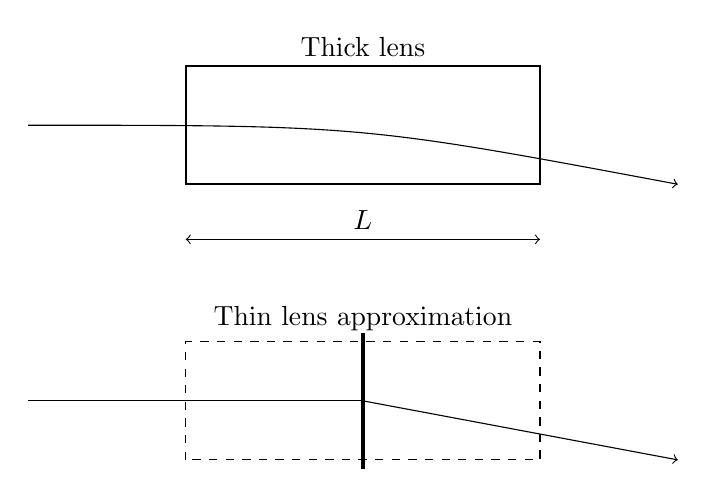
\begin{tikzpicture}
%    \draw[black,thin] (0.0,0.0) grid (16.0,9.0);

    % thick lens 
    \draw[thick] (6.0,4.5) rectangle (10.5,6.0);
    \draw[->] (4.0,5.25) .. controls (8.25,5.25) .. (12.25,4.5);
    \node [rotate=0]  at (8.25,6.25)    {Thick lens};


    %  thin lens
    \draw[dashed]      (6.0,1.0) rectangle (10.5,2.5);
    \draw[<->] (6.0,3.8) -- (10.5,3.8);
    \node [rotate=0]  at (8.25,4.05)    {$L$};

    \draw[thick] (8.24,0.9) rectangle (8.26,2.6);
    \draw (4.0,1.75)  -- (8.25,1.75);
    \draw[->] (8.25,1.75) -- (12.25,1.0);
   \node [rotate=0]  at (8.25,2.80)    {Thin lens approximation};


   
  \end{tikzpicture}
  \caption{Schmematic illustration of the thin lens approximation. The transverse bending of a magnet of length $L$ is approximated by a point-like kick the particle receives only at the center of the magnet. Left and right of the magnet center the particle momentum remaines unchanged.}
  \label{pic:thinlens}
\end{figure}









The analytical treatment of the transfer matrices can be significantly simplified if the magnet length $L$ is small compared to $1/KL$. The magnetic bending can then be treated as a point-like transverse kick which is given to the particle at the center of the magnet, while the the particle trajectory at the rest of the magnet remains undisturbed, so behaves like a drift space (see \figref{pic:thinlens}). Mathematically, this thin lens approximation~\cite{CERN-SL-95-12} corresponds to the limit
\begin{align}
  L \rightarrow 0 \quad \text{with} \quad K \, L = \text{const.} 
\end{align} 
The transfer matrix for a quadrupole magnet simplifies in the thin lens approximation to:
\begin{align}
  \mathcal{M}_{Q,f/d} = \begin{pmatrix}  1 & L \\   KL & 1  \end{pmatrix} \, ,
\end{align}
which is equivalent to the transfer matrix of a thin optical lens with focal length $f=\frac{1}{KL}$.
%
\subsubsection{Periodic Solution and Betatron Motion}
In circular accelerators the quantity $K(s)$ is a periodic quantity with period length $C$:
\begin{align}
K(s) = K(s+C) .
\end{align}
The equation of motion (\ref{eq:hill1}) with periodic $K(s)$ is the Hill differential equation~\cite{wiedemann1999particle}.
The solution of Hill's equation is a quasi-harmonic oscillation 
\begin{align}
x(s) = \sqrt{\tilde{\epsilon}} \, \sqrt{\beta_x(s)} \, \cos \left( \psi(s) + \phi \right) \, , \label{eq:betatron_oscillation}
\end{align}
where $\tilde{\epsilon}$ and $\phi$ are mathematically the integration constants and represent the initial conditions of the particle. The function $\beta_x(s)$ is a periodic function with period $C$, referred to as the betatron function. It is purely defined by the magnetic lattice in the accelerator. 

It defines the maximum local amplitude at a given location. The quantity $\psi(s)$ is the phase of the betatron oscillation defined by
\begin{align}
\psi(s) = \int_0^s \frac{\mathrm{d}s}{\beta(s)} \, .
\end{align}
The total number of betatron oscillations over one turn is the machine tune
%
\begin{align}
  Q = \frac{1}{2 \pi} \int_0^C \frac{\mathrm{d}s}{\beta(s)} \, .
\end{align}
%
%
From \eqref{eq:betatron_oscillation} it can be deduced that $\tilde{\epsilon}$ is a constant of motion\footnote{Note that $\tilde{\epsilon}$ remains constant only if the forces acting on the particle are purely conservative.}, mathematically the Courant-Snyder invariant, for the individual particle:
\begin{align}
\tilde{\epsilon} = \gamma(s) \, x'(s) + 2 \, \alpha(s) \, x(s) \, x'(s) + \beta(s) \, x'^2 (s) \, . \label{eq:parameric_ellipse}
\end{align}
The quantities $\beta(s)$, $\alpha(s)$ and $\gamma(s)$ are the Twiss parameters~\cite{wiedemann1999particle}. They are defined by the beam lattice in the machine. The time derivative of the betatron function $\beta_x(s)$ defines the two other Twiss parameters as:
\begin{align}
\alpha(s) = - \frac{1}{2} \beta'(s) \quad \quad \gamma(s) = \frac{1+\alpha(s)^2}{\beta(s)} \, .
\end{align}

The evolution of an initial set $(\alpha_{x,0},\beta_{x,0},\gamma_{x,0})$ of Twiss parameters in the accelerator depends on the lattice elements and is, equivalent to the transformation of the particle coordinates in \eqref{eq:transfer_matrix}, described by their transfer matrices as follows:
\begin{align}
  \beta_x(s) = C_x^2 \, \beta_{x,0} -2 \, S_x^2 \, C_x^2 \, \alpha_{x,0} + S_x^2 \, \gamma_{x,0} \, .
\end{align}


The expression in \eqref{eq:parameric_ellipse} is the parametric representation of an ellipse in $x,x'$ enclosing a phase space volume of $\pi \tilde{\epsilon}$. Shape and orientation of the phase space ellipse are changing as a function of the the Twiss parameters, but the volume in phase space enclosed by the ellipse remains unchanged (see \figref{fig:phasespace_transformation}). Following \eqref{eq:betatron_oscillation}, the largest possible amplitude in $x$ and $x'$ the particle can reach yields:
%
\begin{align}
  x_\text{max} = \sqrt{\tilde{\epsilon} \, \beta_x(s)} \quad \text{and} \quad x_\text{max}' = - \alpha_x (s) \, \sqrt{\frac{\tilde{\epsilon}}{\beta_x(s)}}
\end{align}

The phase space volume $\tilde{\epsilon}$ is thus related to the peak amplitude of the betatron oscillation for a given $\beta$-function. If many particles compose the beam, the r.m.s. value of the individual $\tilde{\epsilon}$ is referred to as the emittance, which is directly related to the r.m.s. beam size $\sigma_x(s)$:
%
\begin{align}
  \sigma_x (s) = \sqrt{\epsilon_x \, \beta_x} \quad \text{with} \quad \epsilon_x = \langle \tilde{\epsilon_x} \rangle_{\text{rms}} \, .
\end{align}
%
The emittance is a measure for the beam quality and should be as small as possible. It is related to the transverse particle motion, which is reduced due to the relativistic time dilatation. Therefore, the beam emittance decreases proportionally to $\frac{1}{\beta \, \gamma}$ which is known as adiabatic damping. The normalized emittance is defined as 
%
\begin{align}
  \epsilon_N = \epsilon \, \beta \gamma \, ,
\end{align}
and remains constant for all particle energies, assuming that, besides the acceleration, only conservative forces  act on the beam. The emittance is measured in $\mu$m rad.



\begin{figure}[b]  
    \centering
    \includegraphics[width=1\textwidth]{pictures/16021801.pdf}
    \caption{Individual particle trajectories in a periodic quadrupole lattice. The individual betatron amplitude depends on the betatron phase of each particle. The r.m.s. beam envelope is defined by the $\beta$-function and the r.m.s. beam emittance $\epsilon$.}  
    \label{pic:16021801}
    %/home/phermes/Dropbox/PhD/pictures/160217_beam_enveloppe/enveloppe.pdf
\end{figure}


\subsubsection{Solution of the inhomogeneous Equation of Motion}


The solution of the inhomogenious equation of motion \eqref{eq:hill1} is given as
%
\begin{align}
  x(s) = x_h(s) + x_i(s) \, , \label{eq:inhsol}
\end{align}
%
where $x_h(s)$ is the solution of the homogeneous equation shown in \eqref{eq:general_solution} and $x_i$ is one particular solution of the inhomogeneous equation, for example
%
\begin{align}
  x_i(s) = \bar{D}_x(s) \, \delta \, .
\end{align}
%
The dispersion function $\bar{D}_x(s)$ is a periodic function in $s$ with period length $C$, depending on the magnetic elements in the entire ring. It is defined as
%
\begin{align}
  \bar{D}_x (s) = - \frac{\beta_x(s)}{2 \, \sin (\pi \, Q_x)} \, \int_{s_0}^{s_0+C} \, h_x(\tilde{s}) \, \sqrt{\beta(\tilde{s})} \, \cos \left[ 2 \pi \, \left( \psi(\tilde{s}) - \psi(s_0) - \frac{Q_x}{s} \right) \right] \, \mathrm{d} \tilde{s} \, .
\end{align}

In order to be coherent with the definition in the simulation tools used, in the following the dispersion function will be expressed in terms of $D_x(s)$, defined as
%
\begin{align}
  D_x(s) = -\bar{D}_x(s) \, .
\end{align}
%
As shown in \eqref{eq:inhsol}, the dispersion function relates the momentum offset of the particle to an additional transverse amplitude. It thus quantifies the particle deviation due to dispersive effects. Note that this mathematical description represents a linear approximation and higher order dispersive effects are not taken into account. For particles with large momentum offsets, a more accurate description is given by a fully symplectic transformation which can be derived from the accelerator Hamiltonian (see \chapref{chap:hamiltonian}). 



\subsection{Longitudinal Particle Dynamics}

\input{pictures/cavity.tex}

The beams circulating in a high energy synchrotron are bunched, thus there is no continuous current of beam particles through the beam pipe. Rather, dedicated longitudinal slots are assigned for a given number of particle bunches which are populated with the beam particles. The longitudinal bunch spacing and therefore the maximum number of circulating bunches is determined by the accelerating RF cavities which keep the particles in phase at constant energy and accelerate them to the top energy~\cite{wiedemann1999particle}. 

An accelerating cavity operated at an angular frequency $\omega$ provides an electric field given by~\cite{}:
\begin{align}
  V(t) = V_0 \, \sin (\omega \, t) \, .
\end{align}
Using the revolution time $T_S$ of the synchronous particle, the frequency of the RF cavity can be expressed as
\begin{align}
  \omega = h \, \frac{2 \, \pi}{T_S} \, ,
\end{align}
where $\omega$ is chosen such that $h$ is an integer, the harmonic number. The latter condition assures that the synchronous particle is in phase with the RF voltage, such that the energetic kick it receives remains constant. A real particle is not in phase with the RF cavity, but arrives with a certain phase offset
%




\chapter{The Large Hadron Collider}\label{thelhc}
%
%
The Large Hadron Collider (LHC) is the world's largest particle accelerator, designed to store and accelerate proton and \lead beams at unprecedented energies of 7$\,Z\,$TeV. The LHC is a synchrotron of 26.7\,km length, installed in the underground tunnel of the former Large Electron Positron Collider (LEP) at the CERN\footnote{Centre Europ\'{e}en pour la Recherche Nucl\'{e}aire} research center in proximity to Geneva, Switzerland. With the Relativistic Heavy-Ion Collider (RHIC) at the Brookhaven National Laboratory in Long Island (USA), it is one of the two heavy-ion colliders ever built and operated\cite{Fischer2014}. In the first operational period (LHC run 1), the LHC reached energies up to 4$\,Z\,$TeV and collected an integrated luminosity of 29.2\,fb$^{-1}$~\cite{lamont_moyab101} with proton beams and xx.x\,fb$^{-1}$ with \lead beams. With the collected data, the discovery of the long sought Higgs Boson could be announced in July 2012~\cite{higgs:ATLAS,higgs:CMS}. After a phase of machine and detector upgrades from 2013 to 2015, the LHC re-started and accelerated proton beams to the unprecedented energy of $6.5\,$TeV and \lead beams to $6.37\,Z\,$TeV.
%

In this chapter the LHC is presented with the sub-systems relevant for the development of the heavy-ion collimation simulations presented later-on. Particular emphasis is given to the LHC collimation system and the physics processes relevant for heavy-ion collimation.

%
\section{The CERN Accelerator Complex}
%
  \begin{figure}[t]
    \centering
    \includegraphics[width=0.85\textwidth]{pictures/14052201.png}
    \caption{ The CERN Accelerator Complex~\cite{Christiane:1260465}.}  
    \label{pic:14052201}
  \end{figure}
%
The LHC is a high energy synchrotron operated at the end of a complex chain of injectors which pre-accelerate and prepare the beam for its requirements. The ensemble of accelerators which is presently in operation at CERN, referred to as the CERN accelerator complex, is schematially illustrated in Fig.~\ref{pic:14052201}. 

The LHC injector chain originates from two different ion sources, respectively delivering proton or heavy-ion beams. The generation of proton beam starts at a hydrogen ion source feeding the linear accelerator LINAC2, in which the proton beam is accelerated to a momentum of 50~MeV\footnote{For clarity, in this chapter the momementum is given in natural units. All given momenta shall correspond to the correct unit of eV$/c$. Furthermore, the energies for the non fully stripped ions are given in terms of momentum per nucleon, while for the fully stripped ions, the general convention of using the momentum per charge is followed.} and injected in to the Proton Synchrotron Booster. This synchrotron accelerates the beam to 1.4~GeV, the injection energy of the Proton Synchrotron (PS) which provides acceleration up to 25~GeV. After the subsequent injection into the Super Proton Sychrotron (SPS), the beams are brought to 450~GeV, the injection energy of the LHC~\citedr. 
%

Heavy-ion beams originate from the ion source which is connected upstream of the linear accelerator LINAC3. The ions are generated from a block of isotopically pure Pb$^{208}$ by means of an Electron Cyclotron Resonance Source~\cite{CERN-2004-003-V1}. The source delivers ions at a momentum of 2.5\,keV/$A$, which are sent to a spectrometer in order to extract the desired Pb$^{+27}$ charge state. After the filtering, a multi-stage RF system accelerates the selected ion species to a momentum of $4.2\,$MeV/$A$. The following 300~nm thick stripper foil removes more electrons, such that an ion beam of Pb$^{+53}$ is extracted from LINAC3 and transferred to the circular accelerator LEIR (Low Energy Ion Ring). In the latter, the ion beams are cooled, e.g. the transverse emittance is reduced by an adiabatic process using electron scattering. In parallel, the beam is accelerated to a momentum of 72$\,$keV$/A$ at which it is extracted and transferred into the PS. In this machine, the ions bunches are re-shaped and accelerated to a momentum of 5.9$\,$GeV$/A$ and sent to the SPS. Another stripper foil in the transfer line between PS and SPS removes the remaining electrons, such that the ion arriving at the SPS is \lead. The SPS provides the acceleration to the energy of $450\,Z\,$GeV at which the beams are injected into the LHC~\citedr.


\section{LHC Layout}
\subsection{Global Layout}
%
\figref{pic:15032201} shows the LHC layout with its eight straigt insertion regions (IR), four of which host the main experiments (IR1, IR2, IR5 and IR8). The remaining four IRs provide operational functionalities, in particular betatron and momentum cleaning in IR3 and IR7 (see ~\chapref{chap:3}), acceleration in IR4 and the beam dump in IR6. The straight sections are seperated by eight arc regions, in which the particle beams are transported from IR to IR by means of a periodic array of 1232 superconducting dipole magnets and 392 superconducting quadrupole magnets. 
%
%
\begin{figure}[b]
  \centering
  \includegraphics[width=0.7\textwidth]{pictures/15092509.pdf}
  \caption{The layout of the LHC. Based upon \cite{Bruning2012705,CERN-2004-003-V1}.}  
  \label{pic:15032201}
  %/home/phermes/Dropbox/codes/latex/150305_eps2pgf/test.pdf
\end{figure}


\subsection{Insertion Region Layout and Optics}

%IR should be explained in previous section

Each element of the LHC is associated with a cell number, indicating the number of quadrupoles between the closest IP and the respective location. For example the name MQY.4L5.B1 denotes a quadrupole of the MQY type (see \cite{CERN-2004-003-V1}) in cell 4 left of IP5 for Beam 1. 
%
\begin{figure}[b]  
    \centering
    \includegraphics[width=0.9\textwidth]{pictures/16051203.pdf}
    \caption{Optical functions at the experimental insertion IR5 with $\beta^*=1\,$m for a flat machine (no seperation or crossing bump).}  
    \label{pic:16051202}
    %/home/phermes/Dropbox/PhD/pictures/160403_optics/IR5.pdf
\end{figure}
%
The schematic layout of the experimental insertion regions is shown together with the $\beta$ functions in \figref{pic:16051202}. Downstream of the main arcs (1) in which the beams are transported between the IRs, the dispersion suppressor (DS) region (2) serves the purpose of reducing the periodic dispersion function. This is reached by means of a missing dipole structure, in which one of three dipoles is omitted, compared to the nominal dipole structure in the arcs~\citedr. In between the surrounding DS regions, the IR is free of the main dipoles and therefore straight. After the DS, the matching section (3) adjusts the $\beta$ functions to the requirements of the following sections. The separation/recombination dipoles (4) and (5) guide the beams from the separated beam pipes into a common beam pipe. The superconducting triplet magnets (6) provide the final focusing for the experiment at the interaction point (7) (IP) where the beams are brought into collision.

The experiments ATLAS and CMS demand for the highest possible luminosity in order to gain enough statistics for the study of rare processes (see \chapref{chap:lumi}). As discussed later, the luminosity is inversely proportional to the $\beta$ value at the IP (denoted as $\beta^*$), thus the optical lattice is optimized to minimize the $\beta^*$ value. Following Liouville's theorem, small $\beta$ functions imply a large divergence (large $\alpha$ function) at the IP and, due to the absence of magnets between IP and triplet, the $\beta$ functions (and associated with it the beam size) at the superconducting triplets increase with smaller $\beta^*$. The normalized dimensions of the triplet aperture therefore impose a lower limit on the achievable $\beta^*$. This includes effects of adiabatic damping, such that the transition to the smallest $\beta^*$ settings (referred to as squeeze) is performed either at top energy or at the end of the energy ramp (see \chapref{chap:lhccycle}). At injection energy, the optics in IR1 and IR5 are set to $\beta^*=11\,$m while IP2 and IP8 are set to $\beta^*=10\,$m. A summary of the $\beta^*$ values achieved at top energy during the past LHC runs is given in \tabref{tab:betastar}. 
%
%
\begin{table}[htbp]
\centering
\caption{Minimum $\beta^*$ values in LHC operation compared to the design values.}
\label{tab:betastar}
\begin{tabular}{ccccc}
Configuration & Species & \begin{tabular}[c]{@{}c@{}}$\beta^*$\\
IP1/IP5 {[}m{]}\end{tabular} & \begin{tabular}[c]{@{}c@{}}$\beta^*$\\
IP2 {[}m{]}\end{tabular} & \begin{tabular}[c]{@{}c@{}}$\beta^*$\\ IP8
{[}m{]}\end{tabular} \\ \toprule
%
Design & $p$ & 0.55 & 10.0 & 10.0 \\
2011 & $p$ & 1.0 & 10.0 & 3.0     \\
2012 & $p$ & 0.6 & 10.0 & 3.0     \\
2015 & $p$ & 0.8 & 10.0 & 3.0     \\
2016 & $p$ & 0.4 & 10.0 & 3.0     \\ \midrule
Design & Pb & 0.5 & 0.5 & 10.0    \\
2011 & Pb & 1.0 & 1.0 & 3.0       \\
2013 & $p$-Pb & 0.8 & 0.8 & 2.0   \\
2015 & Pb & 0.8 & 0.8 & 3.0       \\ \bottomrule
%
\end{tabular}
\end{table}
%
% table: proton and ion runs, beta*


In the central part of the experimental insertions both beams are moving in a common vacuum pipe to allow for bringing the beams into collision. In order to avoid unwanted collisions of the counter-rotating beams, a seperation bump is applied at every time collisions are not supposed to occur. Furthermore, even when the beams are brought into collision, a crossing bump avoids secondary collisions at parasitic bunch encounters.  The crossing and seperation bumps are, except in IR8, orthogonal to each other. Both bumps are shown for the example of IR5 in \figref{pic:16051204}.

% The closed orbit in the experimental insertions is in general at the center of the beam pipe. Exceptions are  In these regions, the beam orbits are not in the center of the beam pipe to avoid unwanted collisions of the counter-rotating beams. A seperation bump is applied during all phases except when the beams should collide in the IP. The seperation bump is collapsed to establish collisions~\citedr. 

% Depending on the bunch spacing, multiple encounters of the two counter-rotating beams may be localized in the common beam pipe. The application of a crossing bump prevents from parasitic collisions at these secondary bunch encounters.

The functional IRs are not equipped with triplet magnets and the optics is adjusted for the purpose of the installed hardware. The layout, functionality and optics of the collimation insertion regions are shown in \chapref{chap:3}. 
%
%
%
\begin{figure}[htbp]  
    \centering
    \includegraphics[width=0.7\textwidth]{pictures/16051204.pdf}
    \caption{Seperation and crossing bumps in IR5 during the 2011 heavy-ion run with $\beta^*=1\,$m.}  
    \label{pic:16051204}
    %/home/phermes/Dropbox/PhD/pictures/160403_optics/bumps.pdf
\end{figure}
%
%


\subsection{LHC Cycle} \label{chap:lhccycle}
% 
\begin{figure}[b]  
    \centering
    \includegraphics[width=0.8\textwidth]{pictures/16051201.pdf}
    \caption{Beam energy, intensity and $\beta^*$ during the LHC cycle.}  
    \label{pic:16040801}
    %/home/phermes/Dropbox/PhD/pictures/160408_cycle/cycle.pdf
\end{figure}
%

The LHC cycle is a defined operational protocol which ensures safe operation and avoids uncertainties of the magnetic fields which could possibly arise from hysteresis. The LHC cycle is shown for an ideal proton physics fill in \figref{pic:16040801}. 

In the \textit{injection} mode (1) at a beam energy of 450$\,Z\,$GeV, the machine is ready to receive particle bunches from the injectors. The beams are not squeezed in this configuration, to obey the tight aperture restrictions and the optics in the injection insertions IR2 and IR8 are adjusted to optimize the phase advance between the injection septum the injection protection collimators. Once the LHC is filled with beam, the mode is changed to \textit{prepare ramp} (2) in which the injection protection collimators are retracted to allow for the following \textit{ramp} (3), the acceleration to top energy. After the ramp, the \textit{squeeze} (4) is a stepwise optical sequence in which the $\beta^*$ value in the high luminosity IRs is smoothly reduced to the final value for collision. Finally, the beam mode changes to \textit{adjust} (5), in which the seperation bump is collapsed and small additional bumps are introduced to correct for deviations in the closed orbit and maximize the luminosity in the experiments. Once the collisions in the experimental IRs are established, the beam mode is referred to as \textit{stable beams} (6). 
The stable beam mode is maintained for several hours until the luminosity has decreased 
After several hours of stable beams, the beams are dumped (7). The magnets currents are then reduced (ramp down, (7)) to a level below the injection level to eliminate hysteresis effects befor the following injection mode. Note that for heavy-ion operation in 2015, the cycle was adopted from the previous proton run in which the protons had larger rigidities. The ramp down therefore included an increase of the magnet currents from the operational setting at 6.37$\,Z\,$TeV to the proton setting at 6.5$\,$TeV.

In 2015, the formerly distinct steps of ramp and squeeze have been merged to reduce the time to set up the stable beams configuration and thus increase the integrated luminosity. This combined ramp and squeeze synchronously accelerates the beams to 6.5~TeV and reduces the $\beta$ functions at IP1 and IP5 to $\beta^*=3\,$m.



\section{Luminosity} \label{chap:lumi}

An important measure for the performance of a collider is the luminosity. The instantaneous luminosity $\mathcal{L}(t)$ is a time dependent proportionality between the cross section $\sigma_p$ of a physical process and the expected event rate $\frac{\mathrm{d}N_p}{\mathrm{d}t}$ in a given machine configuration~\cite{wiedemann1999particle}:
%
\begin{align}
  \frac{\mathrm{d}N_p (t)}{\mathrm{d}t} = \mathcal{L} \, \sigma_p \, .
\end{align}
%
The luminosity is proportional to the number of bunches $n_b$, the square of the number of particles per bunch $N_P$, the revolution frequency in the machine $f$, the relativistic $\gamma$ (to account for the adiabatic damping) and inversely proportional to the $\beta^*$ value and the normalized emittance:
\begin{align}
  \mathcal{L} = \frac{n_b N_b^2 f \gamma}{4 \pi \epsilon_N \beta^*} \, F \, . \label{eq:lumi}
\end{align}
%
The additional factor $F$ takes into account for the luminosity reduction due to the fact that the colliding bunches are not fully overlapping when a crossing angle $\theta_C$ is applied. The correction factor depends on the longitudinal r.m.s. beam size $\sigma_l$, the transverse beam size at the IP ($\sigma_x=\sigma_y=\sigma^*$) and the crossing angle as follows:
%
\begin{align}
  F = \frac{1}{\sqrt{1+\left(\frac{\sigma^*}{\sigma_l} \, \tan \frac{\theta}{2} \right)}} \, \frac{1}{\sqrt{1+\left(\frac{\sigma_l}{\sigma^*} \, \tan \frac{\theta}{2} \right)}} \,.
\end{align}
%
Following \eqref{eq:lumi}, the luminosity is measured in the unit cm$^{-2}\,$s$^{-1}$. Note that this corresponds to $10^{24}\,\text{b}^{-1} \, \text{s}^{-1}$. The latter expression in combination with the definition given in \eqref{} elegantly illustrates the dependence of the number of expectable events with a cross section $\sigma$ (measured in barns) per time unit. Even more information on the performance of the accelerator can therefore be obtained if the instantaneous luminosity is integrated over the duty time $T$, referred to as the integrated luminosity:
%
\begin{align}
  \mathcal{L}^\text{int} = \int_{0}^T \mathcal{L} \, \mathrm{d} t \, .
\end{align} 
%
Obviously, it is of great interest to enlarge the integrated luminosity to the maximum possible extend, to allow for the study of rare events. This can be done either by increasing the instantaneous luminosity (if not restricted by the experiments) or by optimizing the duty cycle of the machine in order to extend the time the machine is operated in its collision mode (see \chapref{chap:lhccycle}).

\input{pictures/16070312.tex}
  % #PHTHESIS FILE ORIGIN
  %/home/phermes/workspace/tikz/drawing.tex

%
The instantaneous luminosity can be increased if smaller $\beta^*$ values applied, the emittance is reduced, the stored beam intensity is increased or if the luminosity reduction factor is enlarged. While the achievable emittance, number of bunches and bunch intensity depend strongly on the performance of the LHC injectors, the $\beta^*$ value is imposed to an inferior limit due to aperture restrictions. The geometrical luminosity reduction factor $F$ could be improved by reducing the crossing angle, which then interfers with the constraints imposed by the beam-beam interaction.
%

From the hardware side, the latter can possibly be improved by deciated RF cavities, the crab cavities~\cite{}, which are to be installed left and right of the collision point. As shown in \figref{pic:cc} they tilt the colliding bunches to increase their overlap at the collision point. This approach reduces the effective crossing angle and so improves the factor $F$. Crab cavities are not installed in the present LHC configuration, but their installation is foreseen for HL-LHC (see \chapref{chap:hllhc}).







\section{LHC Performance in Operation} \label{chap:lhccycle}
%

\begin{table*}[b]
\centering
\caption{Comparison of the LHC design beam parameters for heavy-ion beams and proton beams in comparison to the parameters typically achieved in the LHC heavy-ion runs.~\cite{CERN-2004-003-V1,pPbref01,jowett-RLIUP13,PbPbref01,Jowett:1492972}. The parameters given for p-Pb operation refer to the \lead beam.}
\label{tab:lhc_parameters}
 \small
\begin{tabular}{cc|cc|cccc}
\multicolumn{2}{c|}{} &  \multicolumn{2}{c|}{Nominal} & \multicolumn{4}{c}{Achieved in the LHC} \\ \toprule

\multicolumn{2}{c|}{Year}     &  &  & 2010 & 2011 & 2013 & 2015 \\% \midrule
\multicolumn{2}{c|}{Species}  & p-p & Pb-Pb & Pb-Pb & \multicolumn{1}{c}{Pb-Pb} & p-Pb & \multicolumn{1}{c}{Pb-Pb} \\ \midrule


$E$          & {[}TeV{]}    & 7 & 7$\,Z$ & 3.5$\,Z$ & 3.5$\, Z$ & 4.0$\, Z$ & 6.37$\,Z$\\

$\gamma$     &              & 7460.5 & 2963.5 & 1481.8 & 1481.8 & 1693.4 & 2696.8\\

$n_b$        &              & 2808 & 592 & 137 & 358 & 338 & 518\\

$n_p$        & {[}$10^8${]} & 1.15$\times 10^{3}$ & 0.7 & 1.12 & $1.20 \pm 0.25$ & $1.40\pm0.27$ & $2.2\pm0.3$\\

$\epsilon_N$ & {[}$\mu$m$\,$rad{]} & 3.75 & 1.5 & 2.0 & $1.7\pm0.2$ & - & $1.50\pm0.15$ \\

$E_s$ &{[}MJ{]} & 362 & 3.81 & 0.71 & 1.98$\pm$0.42 & 2.18$\pm$ 0.42 & 9.54$\pm$1.30\\

$\mathcal{L}_\text{peak}$ &[$10^{27}\,$cm$^{-2}\,$s$^{-1}$] & $1.0\times 10^7$ & \begin{tabular}[c]{@{}l@{}}1 (Pb-Pb)\\ \textit{115}(p-Pb)\end{tabular} & 0.03 & 0.5 & \textit{110} & 3.0\\ 

\bottomrule
\end{tabular}
\end{table*}

% 
The LHC design beam parameters for proton (p) and \lead ion operation are summarized in \tabref{tab:lhc_parameters}. Also the beam parameters so far achieved in LHC operation with heavy-ion beams are presented in this table. In this section a brief overview of the beam parameters achieved in LHC operation so far is given for proton and heavy-ion beams.

\subsection{Proton Beams}

The LHC proton program started with the first data taking phase in 2010. In this first operational period the LHC was operated with small beam intensities at 3.5\,TeV, half the design energy. With the operational experience gained, the stored beam intensity in 2011 could be increased by almost one order of magnitude and a signficiant amount of integrated luminosity was collected. The 2012 proton operation was fully dedicated to luminosity production and the integrated luminosity could be doubled with respect to the predecedent year. In this year the top energy was increased to 4\,TeV~\cite{IPAC16:WEOCA01}.

The luminosity collected in 2011 and half 2012 was already sufficient for the discovery of the Higgs boson~\cite{}. At the beginning of 2013, LHC operation stopped for long shutdown 1 (LS1), a consolidation and upgrade phase with the aim of further increasing the stored beam energy and particle momentum. In 2015, the LHC was re-started and operated at an unprecedented proton energy of 6.5\,TeV. In the following year the LHC operated the first time at nominal luminosity due to the reduced $\beta^*$ value and increased bunch intensity.

\subsection{Heavy-Ion Beams}

The first LHC run with heavy-ions took place in 2010, in which mostly operational experience at 3.5\,$Z\,$TeV was collected and the produced luminosity was unsignificant. The second heavy-ion run in late 2011 was carried out at 3.5\,$Z$\,TeV and delivered half the design luminosity~\cite{PbPbref01}. In 2013 a mixed particle mode was established, in which protons were collided with \lead ions at 4$\,Z\,$TeV~\cite{pPbref01}. This was the first time such asymmetric collisions were achieved in a collider.

The 2015 operational period with heavy ions started with a reference proton run at 2.51$\,$TeV per beam in order to obtain the same center of mass energy as in the p-Pb run of 2013. For the same reason, the ensuing Pb-Pb operation was carried out at an energy of $6.37\,Z\,$TeV, instead of the 6.5$\,Z\,$TeV which would have been possible after the precedenting proton operation at equivalent rigidity~\cite{IPAC16:TUPMW027}. This allows the experiments to compare data at the same center of mass energy for three different collision types: p-p, p-Pb and Pb-Pb. In the 2015 Pb-Pb running period, the LHC outreached the design value of the stored \lead beam energy more than twice, due to the unexpected performance of the LHC injectors reflecting the bunch intensity which has tripled with respect to its design value. This remarkable performance led to an outreach of the design luminosity by a factor three~\cite{IPAC16:TUPMW027}.

\section{The LHC Magnets}

Many different types of magnets provide the guiding and confining forces required for the operation of the LHC. Aside from the magnets in the inner part of the experimental insertions, where the two beams are brought into collision, the LHC magnets are double-bore magnets in which both beams circulate in seperated beam pipes as shown in \figref{pic:16070405}. In this chapter, the superconducting LHC main dipoles and quadrupoles are briefly introduced and their superconducing properties are discussed to motivate the LHC collimation system. More extensive information can be found in \citedr.

\begin{figure}[b]
  \centering
  \begin{tikzpicture}
    \node[anchor=south west,inner sep=0] (image) at (0,0) {\includegraphics[width=0.6\linewidth]{pictures/16070405.png}};
    %\node [draw,rotate=90,x={(image.south east)},y={(image.north west)}]                   at (0.50,0.50)    {text0};
    %\node [draw,rotate=0 ,x={(image.south east)},y={(image.north west)}]                   at (0.22,0.96)    {text1};
    %\node [draw,rotate=0 ,x={(image.south east)},y={(image.north west)},anchor=west]       at (0.22,0.80)    {text2};
    %\draw[->,color=black,thick,x={(image.south east)},y={(image.north west)}]             (0.42,0.22) -- (0.37,0.23);
  \end{tikzpicture}
  \caption{Cross section of the LHC double bore main dipole magnet~\cite{Valeriane:843195}.}  
  \label{pic:16070405}
  %/home/phermes/Desktop/dipole.png
  \end{figure}


\subsection{Main Dipoles}

The 1232 LHC main dipoles are bending magnets of 14.3~m magnetic length capable of delivering a maximum magnetic field of 8.3~T. They are designed for a bending radius of $\rho=\frac{1}{h_x} = ????~\text{m}$ yielding a maximum particle energy of $7\,Z\,$TeV. To provide such large magnetic fields, they are cooled with liquid Helium for an operation at a temperature of 1.9~K. More information on the superconducting LHC dipoles can be found in \citedr.
%
\subsection{Quadrupoles}
The LHC is equipped with many different quadrupoles to provide the focusing required to confine the beams in the LHC arcs and prepare their transverse properties for the collision in the IPs. Depending on their purpose, they are normal or superconducing (and hence provide different field gradients), have different lengths and provide various bore diameters depending on the local aperture requirements~\citedr. 

The beam transport from IR to IR in the LHC arc regions is provided by a structure of 392 alternating focusing and defocusing quadrupoles, which are referred to as the main quadrupoles (MQ). Their maximum magnetic field gradient is 223\,T/m. The superconducting quadrupoles in the matching section of the experimental inserions are of five different types which are summarized in \citedr. The superconducting triplet magnets MQXA and MQXB provide the final focusing for the experiment with a maximum magnetic field gradient of 215\,T/m. 


\subsection{Quench Limit} \label{chap:quenchlim}

The superconducting LHC magnets can be operated in a certain dynamic range, in terms of temperature and external magnetic field. Being a type-II superconductor~\cite{tinkham1996introduction}, their superconducting state can be maintained if the temperature $T$, applied magnetic field $B$ and the current density $J$ in the superconducting cable fulfill certain conditions. The latter can be summarized by a critical surface in the $(T,B,J)$-space underneath of which the magnet is superconducting~\cite{iwasa09}. 

For a given set of two of the three independent parameters, a critical value for the third parameter can be found which then determines the quench limit. As shown in \figref{pic:16070401}, the critical magnetic field for a LHC magnet operated at 1.9\,K for a current density of $J=$1.5$-$2\,kA/mm$^2$ is given by $B_C = 9\,$T, as compared to achievable $B_C=5\,$T at $T=$4.2~K~\cite{bruening:nature07}. Accordingly, the critical temperature is larger if smaller magnetic fields are applied.

\begin{figure}[b]
  \centering
  \begin{tikzpicture}
    \tiny
    \node[anchor=south west,inner sep=0] (image) at (0,0) {\includegraphics[width=0.4\linewidth]{pictures/16070401.jpg}};
    \node [fill=white,rotate=0,x={(image.south east)},y={(image.north west)}]               at (0.88,0.11)    {$T$ [K]};
    %\node [draw,rotate=0 ,x={(image.south east)},y={(image.north west)}]                   at (0.22,0.96)    {text1};
    %\node [draw,rotate=0 ,x={(image.south east)},y={(image.north west)},anchor=west]       at (0.22,0.80)    {text2};
    %\draw[->,color=black,thick,x={(image.south east)},y={(image.north west)}]             (0.42,0.22) -- (0.37,0.23);
  \end{tikzpicture}
  \caption{Critical surface of the superconducting NbTi coils used for the LHC magnets~\cite{courier2013_quench}.}  
  \label{pic:16070401}
  %/home/phermes/Desktop/CCque1_07_13.jpg
  \end{figure}

The superconducting LHC magnets are sensitive to radiation induced heating of their NbTi-coils. They risk to quench if the energy deposited in their coils by impacting beam particles (or their secondary showers) exceeds a defined threshold, referred to as the quench limit. Assuming that the magnetic field and the current density are fixed, the quench is caused by beam-induced heating of the magnet coil. For losses occuring on a short time scale ($<$5\,s), the quench limit is measured in terms of the minimum quench energy density MQED~\cite{PhysRevSTAB.18.061002} in units of mJ/cm$^3$. In contrast, the energy deposited from steady state losses (duration $\geq 5\,$s) is effectively reduced by heat transfer of the superfluid Helium, such that for this scenario the quench limit is quantified by the minimum quench power density (MQPD) in terms of mW/cm$^3$~\cite{lhcprojreport44,PhysRevSTAB.18.061002}. The dependance of these quantities on the loss duration is illustrated in \figref{pic:16070403}.

% An example for simulated quench limits for different energies and loss durations at the LHC MQ magnets is presented in \figref{pic:16070402}. 

So far, beam-induced quenches have only occured in dedicated quench tests, hence have not imposed a limitation in nominal operation with subsequent loss of time and integrated luminosity. However, with the envisaged higher stored beam intensities and constant loss rates, the beam-induced quenches might become a serious issue in the operation of the LHC. 

\begin{figure}[t]
  \centering
  \begin{tikzpicture}
    \node[anchor=south west,inner sep=0] (image) at (0,0) {\includegraphics[width=0.5\linewidth]{pictures/16070403.pdf}};
    %\node [draw,rotate=90,x={(image.south east)},y={(image.north west)}]                   at (0.50,0.50)    {text0};
    %\node [draw,rotate=0 ,x={(image.south east)},y={(image.north west)}]                   at (0.22,0.96)    {text1};
    %\node [draw,rotate=0 ,x={(image.south east)},y={(image.north west)},anchor=west]       at (0.22,0.80)    {text2};
    %\draw[->,color=black,thick,x={(image.south east)},y={(image.north west)}]             (0.42,0.22) -- (0.37,0.23);
  \end{tikzpicture}
  \caption{Simulated quench limits of LHC main dipoles for different loss durations (courtesy of \cite{PhysRevSTAB.18.061002}).}  
  \label{pic:16070403}
  %/home/phermes/Desktop/drawing.pdf
  \end{figure}


\begin{table}[htbp]
  \centering
  \caption{Quench limit estimates for steady state losses at 7\,TeV for the LHC main dipoles.}
  \label{tab:quenchlim}
  \begin{tabular}{lccc} 
    \toprule
    Author           & Reference & MQPD {[}mW/cm$^{3}${]} & Year \\ \midrule
    Auchmann \textit{et al.} & \cite{PhysRevSTAB.18.061002}  & 27-49                  & 2015 \\
    Granieri \textit{et al.} & \cite{IEEE:granieri}          & 47-49                  & 2014 \\
    Bocian \textit{et al.} & \cite{IEEE:bocian}              & 12                     & 2008 \\
    Jeanneret \textit{et al.} & \cite{lhcprojreport44}       & 5                      & 1996 \\ \bottomrule
  \end{tabular}
\end{table}



Reliable predictions of upper intensity limitations due to the risk of quench require accurate estimates of the quench limit. Theoretically, these are not easy to access, because the effective heat transfer to the superconducing coils depends on the geometry of the superconducting coils, the type of insulation, their heat capacities, the rate at which the superconducting helium can remove thermal energy from the coils and many more~\cite{ipac13:THPEA045}. Accordingly, the estimated quench limits are associated to rather large uncertainties and have changed drastically over time when improved simulation models became available and by taking into account experimental data from quench tests. A non-complete summary of the temporal evolution of the estimated quench limits in the MB coils at $7\,$TeV is given in \tabref{tab:quenchlim}.






\section{The LHC Collimation System}\label{chap:3}
%
% \section*{Introduction}
\begin{figure}[b]  
    \centering
    \includegraphics[width=0.6\textwidth]{pictures/16041413.pdf}
    \caption{Design particle momentum and stored beam energy in different particle accelerators. Figure taken from~\cite{collimationsystemref1}.}  
    \label{pic:16041401}
    %/home/phermes/Dropbox/PhD/pictures/160414_beam_energy/drawing-1-compiled.pdf
\end{figure}
%
The LHC is designed to store particle beams of an unprecedented energy (see \figref{pic:16041401}). At design momentum and intensity, the LHC will store protons of a combined energy of 362~MJ per beam, two orders of magnitude more than in previous accelerators~\cite{CERN-2004-003-V1,collimationsystemref1}. 

This energy is sufficient to melt 300~kg of copper. Uncontrolled deposition of the beam energy into the machine hardware can cause severe hardware damage. Even tiny fractions of the LHC beams can cause the superconducting magnets to quench.

Beam particles are subject to a range of physical processes which increase their betatron amplitude, e.g. intra-beam scattering~\cite{Mertens:1364596}, or change their momentum, such as the scattering at the interaction points~\cite{Bruce2014a}. When the resulting betatron amplitude or momentum offset is large enough, these particles can intercept the machine aperture and are lost. Beam losses are thus unavoidable in the operation of the machine. In order to clean the beams from such particles, the LHC is equipped with a multi-stage collimation system. 

This chapter describes the functionality and performance of the LHC collimation system. The physical origins of inefficiencies in the collimation cleaning process are outlined and compared for both proton and heavy-ion beams.  

%

%
%%%%%%%%%%%%%%%%%%%%%%%%%%%%%%%%%%%%%%%%%%%%%%%%%%%%%%%%%%%%%%%%%%%%%%%%%%%%%%%%%%%%%%%%%%%%%%%
%
\subsection{Concept}
%

\input{pictures/16070404.tex}
  % #PHTHESIS FILE ORIGIN
  %/home/phermes/Dropbox/PhD/pictures/160704_collsys/drawing.tex

Given the large particle energies at the LHC, the collimation system requires more than one cleaning instance, because the contradictory requirements of impedance reduction and collimator robustness can not be fulfilled by any known material~\citedr. The three-stage collimation system of the LHC is schematically illustrated at the example of the betatron cleaning insertion IR7 in \figref{pic:15071001}. An overview of the different collimator types is given in \chapref{chap:collimator_types}.

An instance of primary collimators (Target Collimator Primary) serves the purpose of intercepting the primary beam halo (particles of the main beam which are at large amplitudes). In IR7, an horizontal and a vertical TCP provide betatron cleaning in both transverse planes. The TCPs define the global aperture bottleneck and are the collimators closest to the main beam~\citedr. In order to provide enough robustness to withstand a large power load of impacting protons, the active material of the TCPs is a dedicated carbon-fibre composite (CFC)~\citedr. The multi-stage approach relies upon the particle scattering to even larger amplitudes at their passage through the TCP. If a halo particle receives a sufficiently large transverse kick, it is intercepted by the secondary collimators (abb. Target Collimator Secondary, TCS). 

\begin{figure}[t]  
    \centering
    \includegraphics[width=0.6\textwidth]{pictures/16030501.png}
    \caption{Left: Jaw of a secondary collimator. The active material is CFC as for the TCPs. The collimators are water cooled through the copper pipes. Right: Two collimator jaws installed in a collimator tank. Figure taken from ~\cite{Bruce2014a}.}  
    \label{pic:16030501}
    %/home/phermes/Desktop/colli.png
\end{figure}
% 
\begin{figure}[t]  
    \centering
    \includegraphics[width=1.0\textwidth]{pictures/16042009.pdf}
    \includegraphics[width=1.0\textwidth]{pictures/16042007.pdf}
    \caption{Optical functions in the two collimation insertions, IR3 (top) and IR7 (bottom). The vertical black lines represent the locations of the 
      primary collimators}  
    \label{pic:16042001}
    %/home/phermes/Dropbox/PhD/pictures/160403_optics/IR7.pdf
\end{figure}
%
The TCS collimators are retracted with respect to the TCP, thus it should be only exposed to the secondary beam halo with much less intensity than the primary halo. Downstream of the TCS collimators, shower absorbers (TCLA) are installed to protect the superconducting magnets downstream of the collimation IRs from from hadronic and electromagnetic showers generated at the TCS collimators.

Particles can still leak out of the TCS collimators and continue moving inside the machine (tertiary beam halo). In the LHC high luminosity mode with squeezed beams in the experimental insersions, these particles are most likely absorbed in the triplet magnets where the betatronic functions are extreme~\cite{ipac2012:MOPPD062}. In order to avoid beam losses in the triplet magnets, they are protected by the tertiary collimators (abb. Target Collimator Tertiary, TCT). They also provide protection of the experiments from undesired background. The active material of the TCT collimators is tungsten (google: heavy alloy) to provide a high absorption cross section. 

The optical functions in IR7 are optimized for small dispersion functions to intercept only particles at large betatron amplitudes. The momentum collimation region IR3 defines the momentum cut and intercepts particles with momentum offsets beyond a defined threshold. In this region, the optics are matched for a large horizontal dispersion function to intercept the off-momentum particles with the TCP. Contrary to the betatron cleaning, which is carried out for the horizontal, vertical and the skew plane with one dedicated primary collimator each, the principle of momentum cleaning requires a primary collimator only in the horizontal plane. The optical functions for the two LHC cleaning insertions are compared in \figref{pic:16042001}.  

Note that a major inefficiency of the collimation system arises from inelastic interactions in the TCP, where (effectively) off-momentum particles leave the collimator without being captured by the TCS. This is true for both, proton and heavy-ion beams, where for the prior the main production process is single-diffractive dissociation~\cite{ipac10:TUPEB080}. Heavy-ions are subject to fragmentation processes (see \chapref{chap:ionmatterinteraction}) in which fragments with different mass to charge ratios are generated. In both cases, particles with rigidities different from the main beam bypass the secondary collimators and cause high losses in the superconducting magnets of the dispersion suppressor. The IR7 DS magnets are therefore in general the most critical loss location in the LHC ring, in which cleaning inefficiencies of $10^{-2}$ may be reached with heavy-ion beams.


%%%%%%%%%%%%%%%%%%%%%%%%%%%%%%%%%%%%%%%%%%%%%%%%%%%%%%%%%%%%%%%%%%%%%%%%%%%%%%%%%%%%%%%%%%%%%%%
\subsection{Collimator Types} \label{chap:collimator_types}
%
\begin{table}[htbp]
\centering
\caption{Overview of the types of LHC collimators presently installed in the machine (H,V,S: horizontal, vertical, skew)~\citedr.}
\label{tab:ctypes}
\small
\begin{tabular}{lllll}
Type                 & Region    & Name      & Plane & Material \\ \toprule
Primary              & IR3       & TCP       & H     & CFC      \\
Secondary            & IR3       & TCSG      & H     & CFC      \\
Shower Absorbers     & IR3       & TCLA      & H,V   & W        \\ \midrule
Primary              & IR7       & TCP       & H,V,S & CFC      \\
Secondary            & IR7       & TCSG      & H,V,S & CFC      \\
Shower Absorbers     & IR7       & TCLA      & H,V   & W        \\ \midrule
Tertiary             & IR1/2/5/8 & TCT       & H,V   & W        \\
Physics Absorbers    & IR1/5     & TCL       & H     & Cu       \\ \midrule
Dump Protection      & IR6       & TCDQ      & H     & C        \\
Dump Protection      & IR6       & TCSP      & H     & CFC      \\ \midrule
Injection Protection & IR2/8     & TDI       & V     & C        \\
Injection Protection & IR2/8     & TCLI/TCLD & V     & CFC      \\ \bottomrule
\end{tabular}
\end{table}

Besides the presented collimators of the three-stage collimation system, functional collimators are installed for other purposes than halo-cleaning (see \tabref{tab:ctypes}). 

The TDI collimators installed in the two injection insertions IR2 and IR8 protect the LHC hardware from beam loss which could occur due to injection failures. They are composed of graphite in a different alloy than the CFC used for the TCP and TCT collimators. In order to protect a larger area in phase space, the TCLI collimators are installed downstream of the TDI. In case of a dumping failure, multiple components of the LHC could be seriously damaged, in particular the dumping system, magnets downstream of IP6 or even the detector components in the experimental insertions. Therefore, IR6 is equipped with the single-jaw dump protection collimator TCDQ and the double-jaw TCSG collimator (the same collimator type as it is used for the secondary collimators in IR3 and IR7). The jaw of the prior is composed of graphite and is the longest collimator used in the LHC having a length of 6$\,$m. 
For the HL-LHC upgrade additional physics debris collimators, TCLX are forseen to be installed in the experimental insertions. Furthermore, new TCSP collimators with CFC as the active material are to be installed in IR6.


An overview of the different collimator types is given in \tabref{tab:ctypes}. In the design phase of the machine, a progressive upgrade of the LHC collimation system was foreseen to increase the performance of the protection with increasing luminosity and energy~\citedr. 


\newpage
%%%%%%%%%%%%%%%%%%%%%%%%%%%%%%%%%%%%%%%%%%%%%%%%%%%%%%%%%%%%%%%%%%%%%%%%%%%%%%%%%%%%%%%%%%%%%%%
\subsection{Collimator Settings}
%
\begin{table}[b]
\caption{LHC collimator settings applied with squeezed beams at top energy in the LHC heavy ion runs, compared to the design settings. The settings refer to the beam size of proton beams at equivalent energy with a normalized proton beam emittance of $\epsilon_N = 3.5\,\mu$m$\,$rad. }
%
\small
\begin{center}
\begin{minipage}{10cm}
\begin{tabular}{lcccccc}
\toprule
\midrule
 \multicolumn{2}{c}{Collimator} & \multicolumn{5}{c}{Half gap ($\sigma$)} \\
Type & Region & 2010 & 2011 & 2013 & 2015\footnote{Settings refer to a proton energy of $6.5\,$TeV.} & Design\footnote{For design emittance $\epsilon_N=3.75\,\mu$m$\,$rad.} \\ \midrule
TCP  & IR7 & 5.7  & 5.7  & 4.3     & 5.5  & 6.0  \\
TCS  & IR7 & 8.5  & 8.5  & 6.3     & 8.0  & 7.0  \\
TCLA & IR7 & 17.7 & 17.7 & 8.3     & 14.0 & 10.0 \\ \midrule
TCP  & IR3 & 12.0 & 12.0 & 12.0    & 15.0 & 15.0 \\
TCS  & IR3 & 15.6 & 15.6 & 15.6    & 18.0 & 18.0 \\
TCLA & IR3 & 17.6 & 17.6 & 17.6    & 20.0 & 20.0 \\ \midrule
TCT  & IR1/IR2/IR5        & 15.0 & 11.8 &  9.0 & 13.7& 8.3  \\         
TCT  & IR8                & 15.0 & 11.8 &  9.0 & 15.0& 8.3  \\ \midrule \midrule
%\multicolumn{2}{c}{$\epsilon_N$ [$\mu$m rad]} & 1.4 & 1.4 & 1.4 & 1.37 & 1.5 \\
\multicolumn{2}{c}{Heavy-ion energy [$Z\,$TeV]} & 3.5 & 3.5 & 4.0 & 6.37& 7.0 \\
\bottomrule
\end{tabular}
\end{minipage}
\end{center}
\label{tab:14070901}
\end{table}
%
The collimator settings have susceptible influence on the reachable efficiency of the cleaning system yet they must obey numerous contraints:
\begin{itemize}
  \item The risk of damaging the machine hardware, including collimators, must be minimized.
  \item The settings must ensure that the collimation hierarchy is maintained, which implies a smallest achievable retraction between the TCP and TCS collimators. In operation, this requirement led to the application of larger retractions between TCS and TCP than initially foreseen in the design phase.
  \item The triplet aperture must always be protected by the tertiary collimators, which imposes a constraint on the smallest applicable TCT setting. A margin of 1$\,\sigma$ between the measured triplet aperture and the TCT gap is considered to be safe. 
  \item The impedance induced by the collimators can change the tune of the individual particles, which must be taken into account for the collimator settings.
\end{itemize}
%
By convention, the collimator settings are given as the collimator half gap in terms of the normalized beam size. The latter is determined using a normalized emittance of \mbox{$\epsilon_N^p = 3.5\,\mu$m rad} for proton beams. This value was chosen instead of the design emittance at top energy of $3.75\,\mu$m rad because the injectors could deliver a significantly better emittance than initially foreseen~\cite{}. This convention provides consistency and comparability between the runs. The collimator setting in terms of the normalized beam size also takes into account the energy dependence of the geometric emittance due to adiabatic damping. With the collimator settings used in 2015, at top energy the TCP is set to values as small as 1.4~mm, compared to 5.6~mm at injection energy. During the ramp the collimators are synchrously closed to take into account for the decreasing emittance. 

The geometrical collimator settings for heavy-ion operation are so far adopted from the respective precedent proton runs. The emittance of heavy-ion beams is significantly smaller than for proton beams, mainly due to the electron cooling in LEIR. In the LHC Design Report, a heavy-ion emittance of $\epsilon_N^{\text{Pb}} = 1.5\,\mu$m rad is foreseen, which yields the same geometrical emittance as for proton beams at the same rigidity. An exception is the 2015 heavy-ion run at $6.37\,Z$~TeV, in which the geometrical emittance of the previous proton run at $6.5$~TeV were adopted, corresponding to an equivalent heavy-ion emittance of $\epsilon_N = 1.41\,\mu$m rad. 
%
% 
% 



Particles which are not absorbed by the TCPs should be captured by the retracted TCS collimators. This requires that they receive a sufficient transverse angular kick $\Delta x'$ at the TCP, mathematically expressed by the following inequality~\cite{ICOSIMref02}:
%
\begin{align}
  \Delta x' > \sqrt{\frac{(N_P^2 - N_S^2) \, \epsilon_N }{ \gamma \, \beta_x } } \,. \label{dx:secon}
\end{align}
%
Here, $\beta_x$ is the horizontal betatron function at the TCP and $N_P$ and $N_S$ are the applied half gaps of the TCP and TCS respectively. The formula assumes an ideal betatron phase advance between TCP and TCS, such that the particle amplitude at the secondary collimator is maximized.
%

The collimator settings applied during heavy-ion operation with stable beams are compared to the design values in \tabref{tab:14070901}. The settings used so far differ from the design settings and have been modified over the years. The margins between the collimator families were chosen to be increased in order to mitigate measured hierarchy violations\footnote{This applies for proton beams. Based on the measured loss signals in 2011, 2013 and 2015, the cleaning hierarchy with heavy-ion beams is, however, violated. With the smaller beam intensities, this is not considered critical for heavy ions.} during proton operation~\cite{Bruce2014a}. Reasons for such hierarchy violations may be orbit instabilities or beta beating (wrong $\beta$ functions)~\cite{CERN-ATS-NOTE-2011-036MD}. Starting from the conservative settings applied at the beginning of the LHC operation, the settings were continuously optimized and re-set based on operational experience and on the results of dedicated experiments. This includes tightening of the collimator half gaps to allow for smaller $\beta^*$ values~\cite{CERN-ATS-2013-045}.

The reference orbit is not necessarily at the center of the aperture (e.g. when crossing or separation bumps are applied). In this case, the collimators are aligned symmetrically around the reference orbit. In theoretical simulations, the reference orbit is known from the optics computation. During operation with beams, the collimators are aligned using beam based alignment methods~\cite{ipac2011:thpz034} or, for the TCTs, the embedded beam position monitors~\cite{accnote:150028}.



%
\subsection{Particle Losses in the LHC}
%
\subsubsection{Primary Particle Losses}
%
Individual beam particles can be subject to interactions which let the beam emittance grow and populate the primary beam halo leading to continuous losses during operation. Examples for such interactions are intrabeam scattering or interactions of the beam particles with residual gas molecules in the vacuum pipe~\cite{}. Operational reasons for losses can be changes of the optics, beam energy or collimator settings. These losses are typically of short duration. Abnormal losses occur in case of hardware failure and lead to a rapid increase of the loss rate, which triggers to a protection dump by the LHC interlock system~\citedr. The LHC with its collimation system is designed to withstand these different types of losses within different limitations that are specified for each operational configuration~\citedr.

The rate at which particles of the main beam are lost during operation is quantified by the beam lifetime $\tau$, representing the time at which the beam intensity $N(t)$ has dropped to 1/$e$ of its initial value $N_0$:
%
\begin{align}
   N(t) = N_0 \, \exp \left( - \frac{t}{\tau} \right) \, .
\end{align}
%
The instantaneous loss rate $R_L = \frac{\mathrm{d} N(t)}{\mathrm{d}t}$ is related to the beam life time (which is in general time dependent) as follows:
%
\begin{align}
  \tau(t) = \frac{N(t)}{R_L(t)} \, . \label{eq:taudef}
\end{align}
%


The primary collimators are designed to intercept these particles. They can withstand a maximum power load $P_{max}= 487\,\text{kW}$ over 10$\,$s, corresponding to a minimum beam life time of $\tau_\text{min}=720\,\text{s}$ at the design energy of $7\,$TeV~\cite{EPAC02:TUAGB01}. 

\subsubsection{Secondary Particle Losses}

%
\textit{Collimation Debris} 
\\
Secondary collimation losses correspond to particles which have interacted with the collimators and  leave the collimation system without being absorbed in it. If these particles have been subject to significant change of rigidity in the collimators they are likely to be outside of the machine acceptance and absorbed in the aperture of the superconducting magnets where the dispersion increases. This is particularly the case for protons having undergone nuclear interactions, especially single diffractive scattering. Heavy ions can be subject to fragmentation in the collimators, such that the out-coming ion species have large rigidity offsets and are not within the acceptance of the magnet aperture.

The performance of the collimation system is quantified by means of the \textit{local cleaning inefficiency} $\eta(s)$ which relates the integral of the energy from the particles lost in the interval $[s,s+\Delta s]$ to the maximum energy loss (typically at the TCP)
%
\begin{align}
  \eta(s) = \frac{\int_s^{s+\Delta s} E(\tilde{s}) \, \mathrm{d} \tilde{s} }{E_\text{max} \, \Delta s} \, .
\end{align}
%
%
The local cleaning inefficiency allows a simple scaling of the total loss rate to the amount locally lost energy. Following the definition of $\eta(s)$ and \eqref{eq:taudef}, the power $P_L(s,t)$ deposited at the location $s$ with the local cleaning inefficiency $\eta(s)$ is given by
%
%
\begin{align}
  P_L(s,t) = \eta(s) \, \frac{N(t)}{\tau} = \eta(s) \, P_\text{TCP} \, ,
\end{align}
%
where $P_\text{TCP}$ is the power load on the primary collimator.

%
\subsubsection{Losses from interactions at the IP}



\textit{Nuclear Interactions} 

The main focus of the experiments conducted with the beams provided by the LHC is the study of the reaction products generated in nulcear interactions. They occur at the encouter of two particles when impact parameter $b$ is smaller than the sum of the radii of the nuclei involved $b<2\,R$. The particles interact over gluon exchange implying large momentum transfers which may lead to the production of new particles or nuclear fragmentation subsequent to the nuclear excitation of one or both nuclei. At an energy of 7$\,Z\,$TeV, the total cross section for such hadronic interactions of two \lead ions is 8~b~\cite{}. 

A vast variety of secondary ion fragments can continue moving the direction of the main beam and be guided to the aperture of LHC magnets because of their rigidity being incompatible with a confinement from the magnetic lattice. In order to avoid quenches or machine damages from such secondary particles, the high-luminosity insertions IR1 and IR5 are equipped with the TCL collimators dedicated to physics debris absorbtion. 



\textit{Electromagnetic Interactions}\\
Debris from colliding heavy-ions is mainly generated in peripherical collisions at the interaction point in which photon exchange leads to nuclear decomposition or changes in the charge state of the heavy-ion. For LHC energies with \lead ions, the dominating process is bound-free pair production (BFPP)~\cite{}. In this process the involved nuclei interact over the Coulomb force and one or multiple of the exchanged photons creates a virtual pair of leptons from which the negatively charged particle may be captured by one of the interacting nuclei. 

Of practical relevance in terms of cross-section are BFPP processes in which electrons are captured. The BFPP process of $n$-th order for LHC \lead ions is summarized as follows~\cite{BFPP1}:
%
\begin{align}
  \text{BFPP}m:  \quad ^{208}\text{Pb}^{82+} + ^{208}\text{Pb}^{82+} \rightarrow ^{208}\text{Pb}^{82+} + ^{208}\text{Pb}^{(82-m)+} + m \, e^+
\end{align}
%
Compared to the fully stripped nucleus, the $^{208}\text{Pb}^{(82-m)+}$ ion has a different mass to charge ratio and is therefore subject to dispersion. Already the secondary beam generated from first order BFPP is outside the momentum acceptance of the LHC arcs and hence lost at the DS at the end of the IR in which it is produced. 

The exchanged photons can excite one of the nuclei with the residual emission of one or multiple neutrons and/or protons. This process, referred to as electromagnetic dissociation (EMD), shall be discussed in more detail in \chapref{chap:emd}. The $m$-th order process for neutron emission is summarized as follows:
%
\begin{align}
   \text{EMD}m:  \quad ^{208}\text{Pb}^{82+} + ^{208}\text{Pb}^{82+} \rightarrow ^{208}\text{Pb}^{82+} + ^{208-m}\text{Pb}^{82+} + m \, \text{n}
\end{align}
%
The cross sections for electromagnetic interactions are summarized together with the $\chi$ factor quantifying their mass to charge ratio in \tabref{tab:BFPP_cross_section}. 

\begin{table}[h]
\centering
\caption{Cross sections and relative mass to charge ratio of interaction products for electromagnetic and photonuclear interactions of colliding \lead beams at 7$\,Z\,$TeV~\cite{schaum:thesis}.}
\label{tab:BFPP_cross_section}
\begin{tabular}{cccccc}
\toprule
 & BFPP1 & BFPP2 & EMD1 & EMD2 & $\sum$ EMD  \\
$\sigma [b]$ & 281 & 0.006 & 96  & 29 & 226 \\ 
$\chi  $  &  & 0.006 & 96  & 29 & 226 \\ \bottomrule
\end{tabular}
\end{table}

%
With the presented cross section and considering the design luminosity, the secondary BFPP beam carries a power of 26~W. With its distinct rigidity change the secondary BFPP beam impacts the DS magnets in a very localized manner. This leads to a locally high power density in the magnet coils that may cause a quench, as demonstrated in a dedicated BFPP quench test~\cite{}. In 2015 dedicated orbit bumps were used in IR1 and IR5 to steer the secondary BFPP beam into an empty cryostat where the lost particles cannot cause a magnet quench. In the region around the ALICE experiment this solution is not applicable, such that for future operation the installation of additional collimators in the IR2 DS is envisaged~\cite{}. 


%

\reference{http://journals.aps.org/pra/pdf/10.1103/PhysRevA.63.032713}


\subsection{Measurement of Losses in LHC Operation}
%
\begin{figure}[b]  
    \centering
    \includegraphics[width=0.8\textwidth]{pictures/16033101.pdf}
    \caption{Top: Ionization chambers of the LHC BLM sytem, mounted at the LHC Magnets. Bottom: Inner structure of an ionization chamber. Figures taken from \cite{BLM_homepage}.}  
    \label{pic:16033101}
    %/home/phermes/Desktop/pictures/pic.pdf
\end{figure}

The LHC is equipped with more than 4500 ionization chambers, the beam loss monitors (BLM)~\cite{BLMref1,BLMref02}, installed at the outer side of superconduction magnets, collimators and other locations which keep track of the particle losses throughout the ring (see Fig.~\ref{pic:16033101}). The ionization chambers are gas filled cylinders housing a structure of parallel electrodes. Charged particles traversing the detector ionize the gas particles and the created ions and their electrons are captured by the electrodes, which is measured as a drop of the high voltage at which the BLMs are operated. The measured signal is proportional to the radiation dose.
%
%\input{pictures/16070406.tex}
  % #PHTHESIS FILE ORIGIN
  %/home/phermes/Dropbox/PhD/pictures/160704_blms/drawing.tex
%


\begin{figure}[htbp]
  \centering
  \begin{tikzpicture}
    \node[anchor=south west,inner sep=0] (image) at (0,0) {\includegraphics[width=1.0\linewidth]{pictures/16072802.pdf}};

  % \draw[help lines,step=.2] (0,0) grid (16.0,9.0);
  % \draw[help lines,line width=.6pt,step=1] (0,0) grid (16.0,9.0);
  % \foreach \x in {0,1,2,3,4,5,6,7,8,9,10,11,12,13,14,15,16}
  %      \node[anchor=north] at (\x,-0.1) {\x};
  % \foreach \y in {0,1,2,3,4,5,6,7,8,9}
  %     \node[anchor=east] at (-0.2,\y) {\y};

    \node [x={(image.south east)},y={(image.north west)}]                   at (0.07,0.50)    {MBB};
    \node [x={(image.south east)},y={(image.north west)}]                   at (0.23,0.50)    {MQ};
    \node [x={(image.south east)},y={(image.north west)}]                   at (0.48,0.50)    {MBA};
    \node [x={(image.south east)},y={(image.north west)}]                   at (0.83,0.50)    {MBB};
    
    %\node [draw,rotate=0 ,x={(image.south east)},y={(image.north west)}]                   at (0.22,0.96)    {text1};
    %\node [draw,rotate=0 ,x={(image.south east)},y={(image.north west)},anchor=west]       at (0.22,0.80)    {text2};
    %\draw[->,color=black,thick,x={(image.south east)},y={(image.north west)}]             (0.42,0.22) -- (0.37,0.23);
  \end{tikzpicture}
  \caption{BLM positioning around a MQ~\cite{lechner:blmpos}.}  
  \label{pic:16071902}
  %/home/phermes/Desktop/drawing.pdf
  \end{figure}



The BLMs measure the secondary particle showers from the interaction of beam particles with the material of collimators or with the beam pipes and surrounding components. Given their small size, the positioning of the BLMs is essential to monitor losses at strategic locations at which high losses are expected. A schematic illustration of the BLM positioning around the superconducting magnets is shown in \figref{pic:16071902}. 

Measured BLM signals of different BLMs can not be quantitatively compared and related to the number of lost particles per length unit or even to the energy deposited in the magnet coils. With the small azimuthal coverage, the different response function to upstream particle impacts at the beam pipe, the distinct longitudinal distribution of the BLMs and the different loss types throughout the ring, the BLM signals shall be interpreted in the global scale to identify critical loss locations in the machine, rather than deducing quantitative information about energy deposition. The latter requires dedicated simulations, including the shower propagation from the point of primary particle impact~\cite{PAC09:TH5RFP035}. 

Such shower propagation simulations can be combined with quench limit estimates to derive operational thresholds for the BLMs to reduce the risk of undesired quenches or even hardware damage. The BLM data is continuously monitored by the LHC interlock system which triggers a beam dump if these thresholds are exceeded~\cite{guaglio2005reliability}. Both the quench limit and the intensity limit at which the physical dintegrety of the collimators is endangered by beam induced plastic deformations, depend on the time scale at which the losses occur~\cite{bertarelli:chamonix11}. Therefore the signals of the ionization chambers are sampled over twelve different integration time scales reaching from 40\,$\mu$s to $83.89\,$s, denominated as the running sums RS01 to RS12. With increasing integration times, the BLM thresholds are set to larger values, accounting for the larger quench limit with increasing loss duration. 

The longitudinal distribution of losses in the LHC ring is referred to as a loss map. The constant loss monitoring in operation (physics loss map) delivers a convolution of all losses presently occuring, whatever their origin might be. It includes collision debris, such as BFPP losses, collimation losses from intrabeam scattering or modifications of the machine optics in both planes for both beams. 
%
\subsection{Qualification Loss Maps}\label{chap:qualification_lossmaps}

The LHC BLM system is also used to study the efficiency of the collimation system for a given machine configuration. Such analyses are mainly carried out when new optics, collimator settings or particle momenta are commissioned. The cleaning performance must be validated in every possible machine configuration before they are permitted for the injection of high intensity beams~\cite{}. 

Such loss map measurement campaigns are carried out with dedicated bunches (pilot bunches) of reduced intensity with respect to the nominal bunches for stable beams. The circulating bunches are artificially excited to enlarge their transverse emittance, hence the beam particles are intercepted by the collimation system whose debris is measured with the BLMs. This approach produces loss patterns significantly different from nominal operational losses, in which the losses occur for both planes of both beams, indistinguishable with respect to their origin. In the latter scenario, another loss type could be dominating the global loss pattern and, even worse, the collimation losses could be too small to be above the background signal of the BLM system. 

Dedicated strategies to increase the emittance have therefore been developed and are regularly used for loss map measurements. Early loss map measurements have been carried out by means of optics changes that led to tune resonance crossing which induced fast beam losses at the collimation system. From 2012 on, the beam excitation is carried out using the transverse damper (ADT)~\cite{Sapinski:2013wda} which is capable of introducing white noise excitation such that the beam particles receive random transverse kicks resulting in an effective increase of emittance. The latter is distinguished by the better controllability of the excitation which can be selectively carried out in either plane of either beam with a selectable loss rate. 

\reference{https://accelconf.web.cern.ch/accelconf/IPAC2013/papers/mopwo050.pdf}
\reference{https://cds.cern.ch/record/972337/files/lhc-project-report-920.pdf}
\reference{https://accelconf.web.cern.ch/accelconf/HB2012/papers/mop245.pdf}

\subsection{Ion-Matter Interaction} \label{chap:ionmatterinteraction}
Relativistic particles traversing matter are subject to different types of interactions. All of them can be described on a microscopic scale by the interaction of the moving particle (projectile) with the atoms and/or nuclei (target) of the material traversed. The type of intercation that is undergone at the IP often determined by the minimum transverse distance of the projected projecticle trajectory from the target position, the so-called impact parameter $b$, illustrated in \figref{pic:impact}. The impact parameter is often related to the nuclear radii of the target $R_1$ and the \mbox{projectile $R_2$}. 

 \begin{figure}[t]  
  \centering
  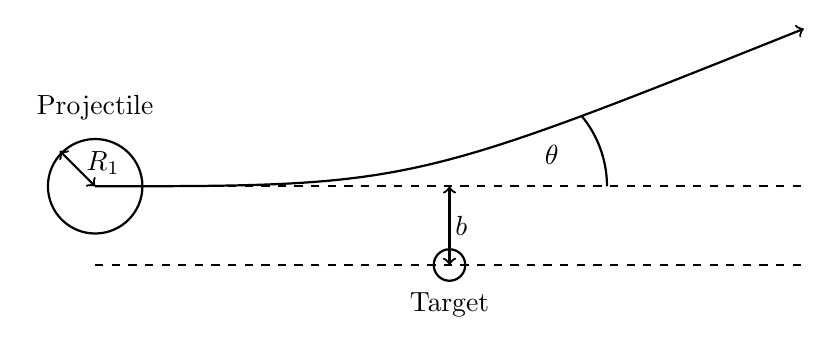
\begin{tikzpicture}
%    \draw[orange,thin] (0.0,0.0) grid (16.0,9.0);

    \draw[->,thick] (2,2) .. controls (6.0,2) .. (11,4);

%    \node [rotate=0,align=left]  at (10,2.7)    {Projected \\ trajectory};
    \draw[dashed,thick] (2,2) -- (11,2);


    \draw[black,thick] (2,2) circle (0.6);
        \draw[<->,thick] (2,2) -- (1.55,2.45);
    \node [rotate=0]  at (2.1,2.3)    {$R_1$};
    \node [rotate=0]  at (2.0,3.0)    {Projectile};
    \draw[<->,thick] (6.5,1) -- (6.5,2);

    % target
    \draw[black,thick] (6.5,1) circle (0.2);
    \draw[black,dashed,thick] (2,1) -- (11,1);
    \node [rotate=0]  at (6.5,0.5)    {Target};
%   \node [rotate=0]  at (6.95,1.1)    {$R_2$};
   \node [rotate=0]  at (6.65,1.5)    {$b$};

   % angle
    \draw[black,thick] (8.5,2) arc (0:40:1.4);
    % \draw[black,dashed,thick] (11,4) -- (11,1);
   \node [rotate=0]  at (7.8,2.4)    {$\theta$};


  \end{tikzpicture}
  \caption{Schematic illustration of the impact parameter.}
  \label{pic:impact}
\end{figure}



\subsubsection{Multiple Coulomb Scattering}

Coulomb scattering occurs when the projectile is deviated from its trajectory while interacting with the coulomb field of the atoms in the collimator material~\cite{Beringer:1900zz}. 

Throughout the passage of the material, the particle can be repeatedly subject to small angular Coulomb scattering and so accumulate an angular deviation significantly larger than from the individual interactions. This process, referred to as Multiple Coulomb Scattering (MCS), can be quantified by the RMS scattering angle $\theta_0$ which is well-described the Moli\`{e}re formula~\cite{Beringer:1900zz}
\begin{align}
\theta_0 = \frac{13.6\,\text{MeV}}{\beta \, c \, p} \, Z \, \sqrt{\frac{\Delta s}{X_0}} \, \left[ 1 + 0.038 \, \ln \left( \frac{\Delta s}{X_0} \right) \right] \, ,
\end{align}
where $\Delta s$ is the distance the particle traversed inside the material and $X_0$ is the radiation length that is a characteristic quantity for the target material. 

The radiation length is accessible via tabulated data or by means of the approximated formula depending on the charge $Z_m$, nucleon number $A_m$ and density $\rho_m$ of the target material~\cite{Beringer:1900zz}
%
\begin{align}
  X_0 = \frac{716.4 \, \text{g} \, \text{cm}^{-2} \, A_m}{\rho_m \, Z_m (Z_m+1) \, \ln (287/\sqrt{Z_m})} \, .
\end{align}
%
The radiation length for the most important collimator materials is given in \tabref{tab:radiation_lengths}.

\begin{table}[t]
\centering
\caption{Properties of the most important collimator materials, including materials foreseen for upgrades of the LHC collimation system. Data taken from~\cite{IPAC15:TUPTY029}.}
\label{tab:radiation_lengths}
\begin{tabular}{lllll}
\toprule
Material & $Z_m$ & $A_m$  & $\rho_m$ {[}g/cm$^3${]} & $X_0$ {[}cm{]}  \\ \midrule
C (CFC)  & 6     & 12.01  & 1.67                    & 25.57          \\
Cu       & 29    & 63.55  & 8.96                    & 1.435          \\
W        & 74    & 183.85 & 19.30                    & 0.35           \\
Mo$_2$C  & 30    & 67.978 & 8.40                     & 1.222         \\ \bottomrule
\end{tabular}
\end{table}

% DATA FROM ELENA FOR FAST IMPLEMENTATION IF NECESSARY
%       element Z       A       rho   X0[g/cm2] X0[cm] 
% 1	Be	4	9.01	1.848	65.19	35.276
% 2	Al	13	26.98	2.7	24.01	8.893
% 3	Cu	29	63.55	8.96	12.86	1.435
% 4	W	74	183.85	19.3	6.76	0.350
% 5	Pb	82	207.19	11.35	6.37	0.561
% 6	C (CFC)	6	12.01	1.67	-	25.57
% 7	C2	6	12.01	4.52	-	9.40
% -	graphite	6	12.01	2.25	42.700	18.978
% -	diamond	6	12.01	3.14	42.700	13.599
% -	B	5	10.8	2.37	52.690	22.232
% -	Ni	28	58.69	8.9	12.680	1.425
% 	O	8	16	-	34.240	-
% -	Al2O3	10	20.392	3.97	27.940	7.038
% 10	Mo	42	95.962	10.22	9.8	0.9589041096
% -	Mo2C	30	67.978	8.4	10.266	1.222
% 8	MoGr	6.653	13.532	2.5	29.828	11.931
% 9	CuCD	11.898	25.238	5.4	17.073	3.162
% 11	Glidcop	28.823	63.149	8.93	12.881	1.442
% 12	Inermet	67.657	166.677	18	6.922	0.385


\subsubsection{Energy Loss from Ionization}

  \begin{figure}[b]
  \centering
  \includegraphics[width=0.85\textwidth]{pictures/15091401.png}
  \caption{Stopping power as described by the Bethe-Bloch formula~\cite{Beringer:1900zz}. Compared to \eqref{eq:bethe}, the mean energy loss per traversed length is normalized by the density of the material.}  
  \label{pic:15091401}
  %/home/phermes/Desktop/lec1.png
  \end{figure}

Particles at the passage through matter can interact inelastically with the electrons of the atoms constituing the target material. At such encounters, a fraction of the projectile's kinetic energy is disposed into the energy required to deliberate an electron from an atom of the target material.

Quantitatively, the mean energy loss per traversed length unit in the material is described by the Bethe-Bloch formula~\cite{Beringer:1900zz}:
\begin{align}
- \left\langle\frac{dE}{dx}\right\rangle = \frac{4 \pi}{m_e c^2} \cdot \frac{nq^2}{\beta^2} \cdot \left(\frac{e}{4\pi\varepsilon_0}\right)^2 \cdot \left[\ln \left(\frac{2 \, m_e c^2 \, \beta^2}{I \cdot (1-\beta^2)}\right) - \beta^2\right] \, , \label{eq:bethe}
\end{align}
where $I$ is the mean excitation energy (which is tabulated for different materials), $m_e$ is the electron rest mass and $n$ is the electron density in the material.


The average energy loss depends on the projectile mass and velocity and on the atomic density of the target. The energy loss is shown as a function of $\beta \gamma$ and the particle type in \figref{pic:15091401}.

\subsubsection{Electromagnetic Dissociation} \label{chap:emd}
Electromagnetic dissociation (EMD) is a photonuclear reaction that occurs at ultraperipherical collisions of the involved nuclei \mbox{($b>R_1 + R_2$)}. The Lorentz contracted electric fields lead to the exchange of a large number of virtual photons which can induce the nuclear excitation of one or both of the involved nuclei~\cite{PhysRevSTAB17021006}. The cross section of the EMD process scales logaritmically with the relativistic $\gamma$ factor of the impacting nucleus~\cite{PhysRevSTAB17021006}. The excited nuclei dissipate the energy under the emission of one or more nucleons, where the emission of neutrons has the largest cross section for heavy nuclei such as \lead. An important example for the electromagnetic dissociation of this isotope is the production of $^{207}$Pb$^{82+}$ in the carbon material of the primary collimators 
\begin{align}
^{208}\text{Pb}^{82+} &+ ^{12}\text{C} \rightarrow ^{207}\text{Pb}^{82+}  + ^{12}\text{C} + n \, .
\end{align}
The residual heavy ion can again be subject to EMD, resulting in $^{206}$Pb$^{82+}$, a main contributor to the ion losses in the aperture of the LHC arcs, as discussed in \chapref{chap:STIER:full}. Overall, the EMD process is very important to consider in the picture of heavy-ion collimation, because the residual ions have rigidities very close to the main beam. They can travel through the magnetic lattice of the LHC over large distances and may cause distinct losses at given LHC elements. 

\subsubsection{Nuclear Interactions}
Nuclear encounters with impact parameters smaller or equal than the sum of the radii of the involved nuclei can lead to interactions over strong force. Whereas the reaction channel is similar to photonuclear interaction, with nuclear excitation of either the target or the projectile and their subsequent disintegration, the spectrum of residual nuclei is much wider when the particle has undergone a nuclear interaction~\cite{bartke:relativistic}. 

Typically residual ion fragments can cover the full isotope spectrum and therefore produce particles with rigidities far from the main beam. For the materials used in primary LHC collimators nuclear interactions occur with cross sections one order of magnitude above the one for EMD processes (see \tabref{tab:xsections} for a comparison) making them an important component in the study of loss patterns of heavy-ion collimaton debris.

Processes of fragmentation, either from EMD or nuclear interactions, come along with deviations in angle and transfer of transverse and longitudinal momentum. The created fragments thus populate not only a wide spectrum in terms of mass and charge, but also of angular coordinate (which can be superior to angular scattering from MCS) and momentum, which leads to additional glazing of the distribution of magnetic rigidities~\cite{PhysRevSTAB17021006}.

\begin{table}[h]
\caption{Cross sections for EMD and nuclear interactions of \lead ions for different fixed target materials at the 2011 LHC energy of $3.5\,Z\,$TeV and its design energy $7.0\,Z\,$TeV~\cite{PhysRevSTAB17021006}.}
\label{tab:xsections}
\centering
\begin{tabular}{ccccc}
  \toprule
       & \multicolumn{2}{c}{\begin{tabular}[c]{@{}c@{}}$\sigma$ {[}b{]}\\ $3.5\,Z\,$TeV\end{tabular}} & \multicolumn{2}{c}{\begin{tabular}[c]{@{}c@{}}$\sigma$ {[}b{]} \\ $7.0\,Z\,$TeV\end{tabular}} \\ \midrule
Target & EMD                                            & Nuclear                                         & EMD                                            & Nuclear                                         \\ \midrule
C      & 0.471                                          & 3.24                                            & 0.498                                          & 3.26                                            \\
Cu     & 10.16                                          & 5.09                                            & 11.05                                          & 5.11                                            \\
W      & 63.52                                          & 6.92                                            & 68.91                                          & 6.95   \\ \bottomrule                                         
\end{tabular}
\end{table}
 

\subsubsection{Nuclear Evaporation and Statistical Fragmentation}

The residual heavy ions generated at a cascade of interactions of either nature may still be in a nuclear charge state above the ground level. Depending on the mass of the fragment two physical processes of energy dissipation can be distiguished. 

Heavy nuclei can decay into their ground state by either nuclear fission, the emission of nucleons or $\gamma$ rays, a process referred to as nuclear evaporation~\cite{HEP2003:MOMT005}. Proton emission from nuclear evaporation is suppressed as compared to neutron emission because of the Coulomb barrier~\cite{HEP2003:MOMT005}.

Light residual ions are subject to fragmentation which can be statistically described by the Fermi breakup model~\cite{fermi:breakup}. In this model, significant momentum can be transferred to the fragments originating from this process.



\begin{table}[htbp]
\caption{Characteristic quantities for the most imporant physical processes of protons and lead ions traversing CFC at 7$\,Z\,$TeV. SCALED with DENSITY. CHECK IF CORRECT. Data partly taken from \cite{ICOSIMref02}.}
\begin{center}
\begin{tabular}{ c c c c }
\toprule
Physics Process & Unit & Proton & \lead \\ \midrule
$- \frac{dE}{E\,\mathrm{d}x}$ & [$10^{-5}$\,m$^{-1}$] & 11 & 917 \\ 
$\theta_\text{MCS}$ &  [$\,\mu$rad/$\sqrt{m}$] & 4.0 & 4.0 \\ 
Nuclear interaction length & [cm] & 47.9 & 3.1 \\ 
EMD length & [cm] & - & 23.9 \\ \bottomrule
\end{tabular}
\end{center}
\label{tab:physics_ions_matter}
\end{table}



\chapter{Simulation Tools}

Important contributions to the excellent performance of the LHC came from theoretical simulations. Many tools have been developed and used to predict various physics aspects of the machine. For collimation, particularly software for particle tracking and simulations of particle-matter interaction are important. The prior requires also a detailed model for optics computation, as the configuration of the magnetic lattice is crucial for the particle motion in the machine. In order to have a complete picture of the collimation efficiency, information must be exchanged between the tracking tool and the particle-matter interaction, which can be realized in different manners. In this chapter, different software tools important for the development of the heavy-ion collimation simulation tools are presented.



\section{MAD-X}
MAD-X (Methodical Accelerator Design)~\cite{MADXref01} is the standard tool to simulate beam dynamics and compute beam optics in particle accelerators. The software is a complete migration of MAD-8 (written in FORTRAN77) to C++ and was introduced in 2002 for the design and simulation of the LHC optics~\cite{MADXref02}.

The software computes the global Twiss parameters by means of transfer matrices for the individual lattice elements. The structure of the machine and the strengths of the magnets are given by the user by means of dedicated input files. A matching function provides the functionality to adjust specific variables such that previously defined constraints are fulfilled. An aperture model of the machine can be processed and compared with the beam position and dimensions to evaluate the available normalized aperture throughout the machine. A dedicated function produces the required optics input for SixTrack (see next Chapter). 



% ----------------------------------- PARTICLE MATTER INTERACTION ----------------------------------

\section{FLUKA}


\begin{figure}[t]  
    \centering
    \includegraphics[width=0.8\textwidth]{pictures/16060102.pdf}
    \caption{FLUKA geometry of the three primary collimators in IR7 for B1~\cite{skordis_fluka_model}.}  
    \label{pic:16031201}
    %/home/phermes/Dropbox/PhD/pictures/160601_fluka_collimators/annotated/coooo_annotated.pdf
\end{figure}


FLUKA (FLuktuierende KAskade) is a fully integrated Monte-Carlo package to simulate particle transport and the interaction of particles with matter~\cite{ferrari2005fluka}. The package simulates the interaction with the nuclei of the traversed material and particles generated in electromagnetic or hadronic cascades are kept track of. The software uses regularly updated physics models derived from experimental data and is used for a variety of simulations, including particle shower simulations and energy deposition studies. 

The species, energy and direction of the incident particles are given by the user in a dedicated input file. The geometry can be defined manually with a dedicated synthax or generated from the FLUKA element database (fedb) which contains LHC elements which may be assembled. The full geometry of the different LHC inserstion regions (see \chapref{}), is available as a FLUKA model and is regularly used to study energy deposition, activation or shower propagation for different beam loss scenarios. As an example, the geometry of three primary LHC collimators, including their mounting plates, is shown in \figref{pic:16031201}.

The FLUKA user input file is a sequence of command lines (called \textit{cards}), which define the simulation setup via different available options~\cite{}. The required output information can be selected, post-processed and written to dedicated files via 38 different user routines that can be linked to the FLUKA executable. Each user routine consists of FORTRAN code that can be adjusted to the specific requirements of the user. The options for pre-defined output can be set in the FLUKA input file by means of the respective card linked to a specific user routine. 


\section{SixTrack}

\subsection{Description}

\begin{figure}[b]
  \centering
  \includegraphics[width=1\textwidth]{pictures/15070701.png}
  \caption{BeamLossPattern algorithm to identify aperture losses SixTrack simulated particle tracks [S. Redaelli, R. Assmann, and G. Robert-Demolaize. Lhc aperture and commissioning
of the collimation system. Proceedings of the LHC Project Workshop
Chamonix XIV, 2005.].}  
  \label{pic:15070701}
  %/home/phermes/Desktop/tra.png
\end{figure}

SixTrack~\cite{SixTrackref01,SixTrackref02,SixTrackref03,SixTrackref04} is designed to provide symplectic six-dimensional tracking of relativistic proton beams in high energy synchrotrons over many turns. Initially developed for dynamic aperture studies, the software is subject to regular updates providing new features for dedicated functions or improved physics models. An important extension is the integrated routine for the simulation of proton collimation in high energy colliders as the LHC~\cite{1591725,collsixtrack}. \

The tracking algorithm is based on symplectic transfer maps derived from the accelerator Hamiltonian, which are implemented in both thick lens model and thin lens approximation~\cite{}. Based on these tracking maps, the array [$x,x',y,y',\sigma,p_\sigma,P$] is transported through the magnetic lattice of the accelerator. The symplecticity makes SixTrack an excellent tool to provide accurate tracking over a large number of turns. 

The collimation subroutine provides an integrated environment for 6D tracking together with a Monte-Carlo Module to simulate the interaction of the protons with the material of the collimation devices. For this purpose, physics models and cross-sections for different types of interactions are implemented for different collimator materials. The SixTrack particle-matter interaction simulation includes energy loss via ionization, multiple Coulomb scattering, and nuclear interactions at the passage of the protons through the collimator. 

In order to identify the loss distribution in the ring, the individual particle tracks are compared to a detailed model of the LHC aperture. If the track of a beam particle is identified to intercept the aperture, the loss location is identified with a precision of 0.1~m and the information is saved in a dedicated output file. The aperture check is first carried out at dedicated aperture markers to reduce the required computing time. Beginning from the marker, particle track is then reversely extrapolated as a straight line and the aperture check is iteratively repeated in steps of $10\,$cm (see \figref{pic:15070701}) until the loss location is indentified.  

In the current SixTrack release version~\footnote{SixTrack Version 4.5.34 from 20.04.2016}, this algorithm is executed on a post-processing level by means of the software BeamLossPattern~\cite{}. Given that all particle tracks have to be saved and analyzed in this approach, this method of loss detection is very time- and space-consuming. A recently developped on-line aperture check~\cite{} compares the simulated proton tracks to the aperture at each tracking step, making the extraction of the particle tracks unnecessary.  

Protons interacting with the collimators are considered to be lost if they undergo nuclear inelastic scattering. A significant amount of losses in the aperture arises from protons having undergone single diffractive scattering. In this process, the proton interacts with a nucleus of the collimator material and is excited to a higher nuclear state. This excited state decays into a proton and other particles and the energy of the outgoing proton is reduced with respect to the incident proton~\cite{}. 

\subsection{Simulation Setup and Running of Collimation SixTrack}
The SixTrack options and input is given via two dedicated input files
\begin{itemize}
  \item fort.2: defining the optical configuration of the accelerator. This file can be automatically generated from MAD-X.
  \item fort.3: Selection of options and beam settings. The most relevant options for collimation studies are the number of tracked particles, number of turns through the machine, particle energy, RF settings, collimator settings and initial distribution. 
\end{itemize}
The COLLIMATION block in the fort.3 file contains information about the settings of the different collimator families. The latter are defined by a collimator database input file, containing information on the name, length and material of the different collimators. The classification of the collimator family is conducted by the prefix of the collimator name and the region where the collimator is installed. 

The initial beam halo can be selected from different options, the most notable ones being an annular halo in $x,x'$ at an amplitude large enough such that the particles hit the primary collimator, or a pencil beam with controlled impact parameter at a given collimator. Even though 

Collimation simulations with SixTrack are usually carried out for 200 turns with an initial sample of 6.4 million protons  starting at IP1. Given the large amount of required space which has to be allocated for the aperture loss detection, and the high amount of required CPU time, the simulations are split into 1000 sub-simulations which are submitted to the CERN batch computing service in which they are processed in parallel, if possible~\cite{}[http://information-technology.web.cern.ch/services/batch]. The post-processing is carried out on the virtual machine of the cluster, such that only the relevant output is saved back in the user directory and the required disk space is reduced by several orders of magnitude. 

% \section{ICOSIM}

% ICOSIM (Ion Collimation Simulation)~\cite{ICOSIMref02,ICOSIMref01} is a tool to simulate the cleaning performance of the collimation system with heavy-ion beams. The tool, which is implemented in Matlab, was developed to evaluate the efficiency of the LHC cleaning system for heavy ions before the start of the LHC.
% It is an integrated program for particle tracking with a Monte-Carlo module to simulate the interaction of heavy-ions with the collimator materials. The tracking routine is based on a matrix multiplication with chromatic modelling in linear approximation and sextupole fields in thin-lens approximation. The information about the magnetic lattice is read from MAD-X output. Along with the tracking, the particle amplitudes are compared to a simplified aperture model, in which the aperture cross sections are approximated by an ellipse. Once the aperture is identified to be intercepted at the end of an element, the exact location is determined by extrapolation, as desribed in the previous chapter. 

% The integrated Monte-Carlo module simulates the interaction of the ions with matter, including energy loss from ionization via the Bethe-Bloch equation and multiple Coulomb scattering, as well as fragmentation processes from EMD and NF~\cite{ICOSIMref02}. The latter is computed using tabulated cross-section information for the two processes which is generated beforehand with FLUKA. When a particle is subject to fragmentation in the collimator, the heaviest fragment is given back to the tracking routine, and transverse momentum transfers from the fragmentation process are not taken into account~\cite{ICOSIMref02}. 

% ICOSIM is equipped with a subroutine to sample the initial distribution, typically a Gaussian distribution in $x,x'$. In order to simulate diffusion, the emittance of the tracked particle bunch is increased by applying random transverse kicks. The simulation is typically carried out over 500 turns for 2 million initial particles. 

\section{SixTrack-FLUKA Coupling}

\begin{figure}[b]  
    \centering
    \includegraphics[width=0.65\textwidth]{pictures/16060101.pdf}
    \caption{Principle of the SixTrack-FLUKA coupling. At every collimator extraction marker (red) the particle bunch is sent to FLUKA where the interaction with the collimator is simulated. The resulting distribution is then re-injected in SixTrack at the injection marker (green), from where the tracking is continued.}  
    \label{pic:16060101}
    %/home/phermes/Dropbox/PhD/pictures/160601_six_fluka_coupling/test/annotated/drawing_annotated.pdf
\end{figure}


The SixTrack-FLUKA online coupling~\cite{mereghetti_ipac2013_1} is a dedicated framework in which the two simulation codes SixTrack and FLUKA are ran in parallel to simulate the cleaning performance of the collimation system by complementary tracking and particle-matter interaction at the collimators. This approach was developed to combine the advantages of both codes with their detailed and regularly updated physics models. The backbone of the particle exchange is a network port which transfers particle information between the two codes while both of them keep running in the background. This shortens the time required normally for subsequent simulations because each code does not have to be re-initialized after each particle exchange and post-processing of data becomes unnecessary. 


\begin{figure}[htbp]
  \centering
  \begin{tikzpicture}
    \node[anchor=south west,inner sep=0] (image) at (0,0) {\includegraphics[width=1.0\linewidth]{pictures/16070701.png}};
    %\node [draw,rotate=90,x={(image.south east)},y={(image.north west)}]                   at (0.50,0.50)    {text0};
    %\node [draw,rotate=0 ,x={(image.south east)},y={(image.north west)}]                   at (0.22,0.96)    {text1};
    %\node [draw,rotate=0 ,x={(image.south east)},y={(image.north west)},anchor=west]       at (0.22,0.80)    {text2};
    %\draw[->,color=black,thick,x={(image.south east)},y={(image.north west)}]             (0.42,0.22) -- (0.37,0.23);
  \end{tikzpicture}
  \caption{Collimator models in the FLUKA input file used for the SixTrack-FLUKA coupling.}  
  \label{pic:16070701}
  %/afs/cern.ch/work/p/phermes/private/150629_coupling_ions/hiSix/160315_HLLHC//home/phermes/Desktop/fedb.png
  \end{figure}



The basic principle of the SixTrack-FLUKA coupling is illustrated in \figref{pic:16060101}. The magnetic lattice used in SixTrack is expanded by additional collimator extraction markers at which SixTrack sends the particle distribution to FLUKA, where the interaction with the collimator is simulated. Conversely, at the end of the collimator, the distribution of residual particles is sent back to SixTrack and re-injected into the lattice at a dedicated injection marker from which the tracking is continued. 

The marker locations correspond to the beginning and end of the collimator tanks. The FEDB stores detailed models of each collimator type (see \figref{pic:16070701}) and the settings of the individual collimators are applied in a dediacted pre-processing algorithm in which the FLUKA input file, required for the coupling simulation, is produced. Every collimator is assigned to a collimator ID. Residual protons which are not identical to the incoming protons (e.g. those produced in nuclear interactions) are assigned to a new particle ID, which can take values up to 2000. 

An important feature required for collimation studies in this framework is an on-line aperture check during the tracking instead of computing the aperture losses on a post-processing level as done in the nominal collimation SixTrack algorithm. Such an on-line aperture check was implemented in 2014. With this algorithm SixTrack continuously compares the particle coordinates to a detailed model of the LHC aperture. With the initial aperture check carried out at the markers, the losses can be more precisely localized by backwards extrapolation, similarly to the aperture check with \texttt{BeamLossPattern}, providing a full comparability of the loss maps generated in collimation SixTrack and with the coupling.

The framework allows for the automatic output of a \texttt{toucMap} file which contains information on the impact position at every collimator. This data can be subsequently used for the detailed shower propagation simulations in FLUKA. With this type of simulation the energy deposited in the regions downstream of the collimators can be calculated by taking into account the contribution of all secondary shower particles. The interaction of the shower particles with the LHC hardware is precisely computed to determine the energy deposited in them. Furthermore, the shower simulations can be used to quantiatively predict the resulting BLM signals. Compared to the nominal cleaning simulations with SixTrack these simulations are extensive in terms of time and space consumptions and are therefore rather carried out for dedicated configurations, e.g. when experimentally measured quench limits shall be theoretically accessed.


%\chapter{Collimation at the LHC}\label{chap:3}
%
\section*{Introduction}
%
At design energy and beam intensity, the LHC stores proton beams with a combined energy of $2 \times $362$\,$MJ~\cite{CERN-2004-003-V1}, corresponding to the amount of energy required to melt 600$\,$kg of copper. Besides the highly destructive potential of such energetic beams, which could cause serious damage at LHC components, already tiny amounts of this energy suffice to quench the superconducting LHC magnets~\cite{}. Such quenches are undesired because they interrupt the operation of the machine and reduce the time available to collect integrated luminosity for the experiments and therefore the statistics for rare events occuring at the particle collisions. 

Many processes continuously scatter beam particles to large transverse amplitudes or cause them to lose fractions of their momentum. One example for these processes is intra-beam scattering (IBS). Particles which have been scattered to such large amplitudes compose a beam halo which continues moving inside the machine. If no countermeasures are taken, these halo particles are scattered further outside until they have reached a large enough amplitude to be absorbed at the global machine aperture bottleneck. The processes which continuously re-populate the beam halo can not be avoided such that beam losses during machine operation become unpreventable. 

The ensemble of particles at betatronic amplitudes far from those of the beam core are referred to as the beam halo. In order to avoid uncontrolled losses of such halo particles, they are removed from the beam by intercepting them with a set of dedicated solid devices, the LHC collimation system. 

In this chapter, the design, functionality and performance of the LHC collimation system are discussed for both, proton and heavy-ion beams.



%
\section{The LHC Collimation System}
\subsection{Concept}
  \begin{figure}[t]
  \centering
  \includegraphics[width=1.0\textwidth]{pictures/15071301.pdf}
  \caption{Schematics of the LHC multi stage collimation system. Particles at large betatronic amplitudes are intercepted by the primary collimators (TCP) from which they should be scattered to even larger amplitudes to be captured by the secondary collimators (TCS), which are equipped with dedicated shower absorbers (TCLA). Particles escaping from the TCS constitute a tertiary beam halo which would be absorbed in the global aperture bottleneck, which are the superconducting triplet magnets in the experimental insertions. Therefore, the latter are protected with the tertiary collimators (TCT). Particles which have lost energy but have not been scattered enough in the TCP can still bypass the TCS and are most likely absorbed in the dipole magnets of the LHC arcs, where the dispersion rises.}  
  \label{pic:15071001}
  %/home/phermes/Dropbox/PhD/pictures/collimationsystem_drawing_thesis/drawing2.pdf
  \end{figure}

The aim of the system is the interception and controlled absorption of the transverse beam halo which is continuously re-populated during operation~\cite{}. In other accelerators, such halo particles can be intercepted and absorbed by means of collimators with two movable jaws that are brought closely to the beam center~\cite{}. Contrary to such low-energy machines, the highly energetic and destructive LHC beam halo can not be removed from the beam by means of a single collimation unit. With the high particle momenta and the large stored beam energies, no known material possesses a large enough absorption cross section and radiation hardness to immediately stop halo particles circulating in the LHC. Therefore, the LHC is equipped with a three-stage collimation system which is schematically illustrated for the example of the betatron cleaning insertion IR7 in \figref{pic:15071001}.

The primary beam halo of particles at large betatronic amplitudes is intercepted with the primary collimator (abb. Target   Collimator  Primary, TCP). This collimator type is the only collimator which should be exposed to the main beam. In order to provide enough radiation hardness, the collimator jaws are composed of a dedicated carbon-fibre composite (CFC). The collimation system relies upon the scattering of the halo particles at their passage through the CFC to even larger betatronic amplitudes. If a halo particle receives a sufficiently large transverse kick, it is intercepted by the secondary collimators (abb. Target Collimator Secondary, TCS). 

The TCS collimators are retracted with respect to the TCP, thus it should be only exposed to the secondary beam halo which carries a significantly lower amount of energy. Compared to the TCP collimators of 0.6$\,$m length, the TCS collimators are significantly longer being 1$\,$m long. Downstream of the TCS collimators, the secondary shower absorbers shall provide protection from particle showers arising from the interaction with the TCS.

Scattered particles can still leak out of the TCS collimators and continue moving inside the machine (the so-called tertiary beam halo). In the LHC high luminosity mode with squeezed beams in the experimental insersions, these particles are most likely absorbed in the triplet magnets where the betatronic functions are extreme. In order to avoid beam losses in the triplet magnets, they are protected by the tertiary collimators (abb. Target Collimator Tertiary, TCT). This collimator type consists of copper to provide a high absorption cross section. The three described stages compose the three stage collimation system of the LHC.

\begin{figure}
\centering
\resizebox{1.0\textwidth}{!}{\input{pictures/14121239.pgf}}
\resizebox{1.0\textwidth}{!}{\input{pictures/14121503.pgf}}
%\resizebox{1.0\textwidth}{!}{\input{pictures/14121222.pgf}}
\caption{Optical functions in the two LHC collimation insertions.}
\label{pic:14121222}
\end{figure}

The functionality of the momentum cleaning insertion in IR3 is the same as for IR7, with the difference that the optics in IR7 is matched for large betatronic functions at the TCP, while in IR3 it is matched for a larger dispersion function (see \figref{pic:14121222} for a comparison). In consequence, the TCP in IR3 intercepts off-momentum particles rather than particles at large betatronic amplitudes. 

Besides the presented collimators of the three-stage collimation system, functional collimators are installed for other purposes than halo-cleaning. The TDI collimators installed in the two injection insertions IR2 and IR8 protect the LHC hardware from beam loss which could occur due to injection failures. They are composed of graphite in a different alloy than the CFC used for the TCP and TCT collimators. In order to protect a larger area in phase space, the TCLI collimators are installed downstream of the TDI. In case of a dumping failure, multiple components of the LHC could be seriously damaged, in particular the dumping system, magnets downstream of IP6 or even the detector components in the experimental insertions. Therefore, IR6 is equipped with the single-jaw dump protection collimator TCDQ and the double-jaw TCSG collimator (the same collimator type as it is used for the secondary collimators in IR3 and IR7). The jaw of the prior is composed of graphite and is the longest collimator used in the LHC having a length of 6$\,$m. 

An overview of the different collimator types is given in \tabref{tab:collimator_types}. In the design phase of the machine, a progressive upgrade of the LHC collimation system was foreseen to increase the performance of the protection with increasing luminosity and energy~\citedr. 


 \subsection{Collimator Settings}


\begin{table}[htbp]
\caption{LHC collimator settings applied in the LHC heavy ion runs compared to the design settings. }
\begin{center}
\begin{tabular}{lcccccc}
\toprule
\midrule
 \multicolumn{2}{c}{Collimator} & \multicolumn{4}{c}{Half gap ($\sigma$)} \\
Type & Region & 2010 & 2011 & 2013 & 2015 & Design \\ \midrule
TCP  & IR7 & 5.7  & 5.7  & 4.3  & 9.9 & 6.0  \\
TCS  & IR7 & 8.5  & 8.5  & 6.3  & 9.9 & 7.0  \\
TCLA & IR7 & 17.7 & 17.7 & 8.3  & 9.9 & 10.0 \\ \midrule
TCP  & IR3 & 12.0 & 12.0 & 12.0 & 9.9 & 15.0 \\
TCS  & IR3 & 15.6 & 15.6 & 15.6 & 9.9 & 18.0 \\
TCLA & IR3 & 17.6 & 17.6 & 17.6 & 9.9 & 20.0 \\ \midrule
TCT  & IR1/IR2/IR5/IR8    & 15.0 & 11.8 &  9.0 & 9.9 & 8.3  \\ \midrule 
 \multicolumn{2}{c}{Energy [TeV]} & 3.5 & 3.5 & 4.0 & 6.5 & 7.0 \\
\bottomrule
\end{tabular}
\end{center}
\label{tab:14070901}
\end{table}

The multi-stage collimation system relies upon the scattering of the halo-particles 

The functionality of the LHC betatron cleaning system is schematically illustrated in \figref{pic:14052202}. In the collimation regions IR3 and IR7, primary collimators (TCPs) are set to a collimator opening of $N_1$ (transverse distance from beam centre expressed in terms of $\sigma$) to intercept the trajectories of particles at large amplitudes. These particles interact with the collimator material, such that they are either scattered back into the beam or to a larger amplitude~\citedr.\

Depending on the angular kick, the latter can then intercept the secondary collimators (TCS) of opening $N_2$, which is slightly retracted with respect to the TCPs ($N_2>N_1$). This is provided, if the angular kick $\Delta x'$ fulfills the condition~\cite{jeanneret1998optics}

\begin{align}
\Delta x' > \sqrt{\frac{(N_1^2 - N_2^2) \, \epsilon_N }{ \gamma \, \beta_x } } \,,
\end{align}
where $\epsilon_N$ is the transverse normalized emittance, $\beta_x$ is the horizontal optical $\beta$-function at the primary collimator and $\gamma$ is the Lorentz factor.


\section{Measurement of Losses during LHC Operation}

The LHC is equipped with more than 4500 ionization chambers, the beam loss monitors (BLM)~\cite{BLMref1,BLMref02}, installed at the outer side of superconduction magnets, collimators and other locations which keep track of the particle losses at the particular locations. The ionization chambers measure secondary particle showers arising from the interaction of the ultra-relativistic particles interacting with the collimator material or with the beam pipe and surrounding components if they are lost. The BLM data is continuously monitored by the LHC interlock system which triggers a beam dump if a certain loss threshold is exceeded~\cite{guaglio2005reliability}. This is done to protect the machine from beam damage e.g. in the case of sudden instabilities or changes in the beam configuration inducing too much losses. Also losses of collisional debris can be monitored with this system. The so-obtained data is used to show the longitudinal distribution of losses as a so-called physics loss map.

Besides the monitoring of the losses in operation, the BLM system can be used for a dedicated evaluation of the cleaning efficiency of the collimation system if the beams are excited to large transverse amplitudes or purposely momentum shifted by the RF system. This kind of measurement is described in the following as a qualification loss map.

\subsection{The LHC Beam Loss Monitors}
\begin{figure}[t]
  \centering
   \def\svgwidth{1.0\linewidth}
   \input{pictures/hybrid_pictures/14062001.pdf_tex}
  \caption{Illustrated positioning of BLMs at a superconducting LHC magnet~\cite{dehning2002lhc}.}
\label{pic:14061701}
\end{figure}
%
The BLMs used at the LHC are ionization gas detectors of cylindrical shape, which are installed outside the beam pipe. They measure the particle showers which are produced by a particle hitting the LHC beam pipe.
Inherently, the BLMs do not provide full azimutal or longitudinal coverage, such that the BLM response for the same amount of lost particles may vary between two different locations. Thus, the comparability of experimental measurements of the distribution of loss positions in the machine (lossmaps) with simulation data is therefore limited. Also, the translation of BLM signals into magnet heating and therefore the quench limit in terms of BLM signal is not trivial. Dedicated monte carlo simulations are necessary, in order to estimate the heating at a specific magnet due to a specific configuration of initial particle hits, under respect of the individual magnet geometry. However, the measurements give a very good idea of frequent loss positions and approximately the expectable loss intensity. 


\subsection{Physics Loss Maps}

During operation of the LHC, the losses in the machine are continuously monitored. The losses observed in this case arise from many different effects, the most important ones are summarized in the following:
%
\paragraph{Collimation losses} Different physical processes continuously re-populate the beam halo or lead to an energy loss of the involved particles. These particles should be intercepted by the LHC collimation system. The losses are registered by the BLMs installed at the collimators. Furthermore losses at the magnets arise from particles escaping from the collimation system. 
%
\paragraph{Losses from temporary instabilities} Furthermore, changes of magnet strengths, for example occuring during the ramp or squeeze, may lead to temporary instabilities causing losses that can be monitored by means of the BLM system. 
%
\paragraph{Physics debris} Debris from the experiments can involve [...] for protons. For the case of heavy-ions important debris arises from the bound free pair production (BFPP) process from the interaction of two \lead ions closely encountering each other at the interaction point. During the encounter of the two particles, an electron-positron pair is produced by the exchanged photon. The electron is then captured by the electron shell of one of the two involved nuclei:
\begin{align}
^{208}\text{Pb}^{82+} + ^{208}\text{Pb}^{82+} \rightarrow ^{208}\text{Pb}^{82+} + ^{208}\text{Pb}^{81+} + e^+ \, .
\end{align}
Compared to the fully stripped nucleus, the $^{208}\text{Pb}^{81+}$ ion possesses a different mass to charge ratio and is thus subject to dispersion. The ion is lost at the DS at the end of the IR. Owing to the large cross section of the process, the BFPP loss is dominant in the physics loss map during heavy-ion operation.

Examples for physics loss maps are shown for the case of proton and heavy-ion beams in \figref{fig:physics_loss_maps1}. In the measured loss map the contributions from the two beams can not be distinguished. Also, it is in general not trivial to de-convolute the contributions of the different processes described above. 
%
\subsection{Qualification Loss Maps}


In order to selectively study the cleaning efficiency of the LHC collimation system the collimation losses must dominate in the loss maps.


[] AC Dipole for beam excitation
[] Resonance crossing techniques



\section{Collimation of Heavy-Ion Beams at the LHC}

At their passage through matter, heavy ions interact differently than protons. Instead of being mainly scattered to larger transverse amplitudes as it is the case for protons, ions are less subject to scattering but have large cross-sections for the fragmentation into other isotopes.  In this section the interaction of ions with matter is discussed and the consequences on the collimation efficiency are outlined. The collimation efficiency measured at the LHC is compared for heavy-ion beams and proton beams.


\subsection{Heavy-Ion Qualification Loss Maps}

\begin{figure}[b]
  \begin{center}
\begin{minipage}[t]{0.49\textwidth}
\includegraphics[width=1\textwidth]{pictures/15091803.pdf}
\end{minipage}
\begin{minipage}[t]{0.49\textwidth}
\includegraphics[width=1\textwidth]{pictures/15091802.pdf}
\end{minipage}
%\includegraphics[width=0.49\textwidth]{pictures/15091801.pdf}
%\includegraphics[width=0.49\textwidth]{pictures/15091802.pdf}
\caption{Qualification loss maps with proton and \lead beams at $3.5\,Z\,$TeV with identical collimator settings and optics, except in IR2. The proton loss map is taken from \cite{Bruce2014a}. Both measurements were taken during the 2011 proton and heavy-ion operation. The vertical dashed lines mark the LHC octants. The upper plots show the full LHC ring, the bottom plots a zoom to IR7.}
\label{fig:meas_lm_comparison}
  \end{center}
\end{figure}


In Fig.~\ref{fig:meas_lm_comparison} qualification loss maps are compared from measurements taken in 2011 with heavy-ion beams and proton beams at energies of $3.5\,Z\,$TeV with identical optical und collimator settings, except in IR2. In the latter, heavy-ion beams were squeezed to \mbox{$\beta^*=0.8\,$m} instead of the $\beta^*=10\,$m applied for protons. The applied collimator settings are summarized in Tab.~\ref{tab:14070901}. As usual, all BLM signals are normalized to the highest signal, typically seen at the TCP or just downstream. 

\textit{The heavy-ion loss distribution is dominated by losses in the betatron collimators of IR7, followed by the momentum collimators in IR3. Downstream of the betatron collimation region, two loss clusters in the dispersion suppressor region were measured at amplitudes of $\eta_\text{max} = 10^{-2}$ (two orders of magnitude larger than the DS loss clusters for protons). Four loss peaks at $\eta_\text{max} = 10^{-4} - 10^{-2}$ are present downstream of the dispersion suppressor in the arc magnets between IR7 and IR8. The losses at the TCT in IR8 are smaller with heavy-ion beams than for proton beams. Two loss peaks in the arc region between IR8 and IR1 are visible in both loss maps, but is larger by 2-3 orders of magnitude for the heavy-ion beam. The TCT losses in IR1 are followed by a large loss peak in the arc region between IR1 and IR2, with $\eta_\text{max}=10^{-3}$. While IR2 is free of losses beyond the noise level in the proton loss map, four major loss peaks, one being at the TCT, are visible in octant 2 with the heavy-ion beams. The difference loss patterns in this region can be explained from the different optical configuration used in the two measurements. The loss rate in IR3 is larger by 2 orders of magnitude for the heavy-ion case, indicating the large amount of effectively off-momentum ions which is present in the machine. The losses at the IR5 TCT and the dump protection devices in IR6 are higher with proton beams than with heavy-ion beams.}

In the IR7 DS, the collimation efficiency for heavy-ion beams is worse by two orders of magnitude with respect to proton beams. 



\begin{table}[htbp]
\caption{Physics processed of protons and lead ions in the collimator material, with characteristic quantities~\cite{braun2004collimation}.}
\begin{center}
\begin{tabular}{ l c c }
\toprule
Physics Process & Proton & \lead \\ \midrule
$\frac{dE}{E\,\mathrm{d}x}$ due to ionization & -0.0088\%/m & -0.73\%/m \\ 
Multiple Scattering (projectred r.m.s. angle) & 4.72$\,\mu$rad/$\sqrt{m}$ & 4.72$\,\mu$rad/$\sqrt{m}$ \\ 
Nuclear Interaction length ($\approx$ fragmentation length) & 38.1$\,$cm & 2.5$\,$cm \\ 
Electromagnetic dissociation length & - & 19$\,$cm \\ \bottomrule
\end{tabular}
\end{center}
\label{}
\end{table}

\subsection{Ion-Matter Interaction} \label{chap:ionmatterinteraction}

Ultrarelativistic ions interact (collide) with the atoms of the traversed material in different manners. Such collisions do not require a physical overlap of the involving particles, but it is sufficient if the impact parameter $b$ (the smallest distance between the projectile and the target) is small enough such that a strong or electromagnetic interaction can take place. 

\subsubsection{Energy Loss from Ionization}

  \begin{figure}[b]
  \centering
  \includegraphics[width=0.85\textwidth]{pictures/15091401.png}
  \caption{}  
  \label{pic:15091401}
  %/home/phermes/Desktop/lec1.png
  \end{figure}

Particles at the passage through matter can interact inelastically with the electrons of the constituing atoms. At such encounters, the target atoms are ionized and the liberated electron receives a fraction of the projectile's kinetic energy. This energy loss is described by the Bethe-Bloch formula:
\begin{align}
- \left\langle\frac{dE}{dx}\right\rangle = \frac{4 \pi}{m_e c^2} \cdot \frac{nz^2}{\beta^2} \cdot \left(\frac{e^2}{4\pi\varepsilon_0}\right)^2 \cdot \left[\ln \left(\frac{2m_e c^2 \beta^2}{I \cdot (1-\beta^2)}\right) - \beta^2\right]
\end{align} \, .
The average energy loss depends on the projectile mass and velocity and on the atomic density of the target. The energy loss is shown in function of $\beta \gamma$ and the particle type in \figref{pic:15091401}.

\subsubsection{Electromagnetic Dissociation}
Electromagnetic dissociation occurs at ultraperipherical collisions of the involved nuclei ($b>R_1 + R_2$). The Lorentz contracted electric fields lead to the exchange of a large number of virtual photons that can induce the nuclear excitation of one or both of the involved nuclei. The excited nuclei decay under the emission of one or more nucleons, where the emission of neutrons has the largest cross section for heavy nuclei such as \lead. An important example for the electromagnetic dissociation of lead is the production of $^{207}$Pb$^{82+}$ in the carbon material of the primary collimators 
\begin{align}
^{208}\text{Pb}^{82+} &+ ^{12}\text{C} \rightarrow ^{207}\text{Pb}^{82+}  + ^{12}\text{C} + n \, .
\end{align}
The resulting heavy ion can be subject to a sub-sequent EMD resulting in $^{206}$Pb$^{82+}$, a main contributor to the ion losses in the aperture of the LHC arcs, as discussed in \chapref{chap:isocontributions}.

\subsubsection{Nuclear Fragmentation}
Nuclear encounters with impact parameters smaller or equal than the sum of the radii of the involved nuclei can lead to interactions by means of the strong force. One or both of the overlapping nuclei desintegrate typically into many different nuclear fragments. The particular composition of isotopes generated by such an interaction is different for every interaction. 

\subsubsection{Multiple Coulomb Scattering}

Coulomb scattering occurs if the projectile is deviated from its trajectory while interacting with the coulomb field of the atoms in the collimator material.This elastic scattering can occur many times throughout the passage through the collimator materials, thus the many small scattering angles can superimpose to a larger final angle at exit of the material. The RMS angle due to multiple Coulomb scattering is well-described by the Moliere formula~\cite{Beringer:1900zz}
\begin{align}
\theta_0 = \frac{13.6\,\text{MeV}}{\beta \, c \, p} \, Z \, \sqrt{\frac{\Delta s}{X_0}} \, \left[ 1 + 0.038 \, \ln \left( \frac{\Delta s}{X_0} \right) \right] \, ,
\end{align}
where $\beta\,c = v$ and $p$ are particle speed and momentum, $\Delta s$ is the distance the particle traversed inside the material, $Z$ is the charge of the beam particle and $X_0$ is the characteristic scattering length (see \chapref{xxx}). The latter is depending on the material and is either accessible via tabulated data or by means of the approximated formula in function of the charge $Z_m$ and nucleon number $A_m$ of the atoms constituing the material:
\begin{align}
X_0 = \frac{716.4 \, A_m}{Z_m (Z_m+1) \, \ln (287/\sqrt{Z_m})} \, .
\end{align}


\subsection{Fragmentation and Scattering at the Primary Collimators}

 \begin{figure}[b]
 \begin{minipage}[t]{0.5\textwidth}
 \includegraphics[width=1\textwidth]{pictures/15091301.pdf}
 \end{minipage}
 \begin{minipage}[t]{0.5\textwidth}
 \includegraphics[width=1\textwidth]{pictures/15091003.pdf}
 \end{minipage}
 \caption{Comparison of the distribution $P_\text{eff}$ and the scattering angle of particles leaking out the TCP carbon material between a proton beam (top) and a heavy-ion beam (bottom). The simulation was carried out using FLUKA at an energy 3.5$\,Z\,$TeV with the beam impacting perpendicularly at a carbon target of thickness $10.3\,$cm. The thickness corresponds to the interaction length in the TCP material with an impact parameter of $b=3\,\mu$m (see Sec.~\ref{chap:stier_description}).} %The black lines indicate $\pm \Delta \theta_\text{min}$ as shown in Eq.~(\ref{minkick}). Ions with $\Delta \theta$ between the two lines are not captured by the secondary collimators. }
 \label{fig:15022301}
 \end{figure}




The momentum per nucleon $p=P/A$ and the transverse angle of the fragment trajectories $\theta$ therefore acquire offsets of $\Delta p,\Delta \theta$ with respect to the heavy-ion which initially impacted the collimator material.



\begin{figure}[b]
  \begin{center}
\includegraphics[width=0.65\textwidth]{pictures/15091004.pdf}
\caption{Energy fraction of particles leaking out of the primary collimator which are uncaptured by the secondary collimators. Simulation carried out by FLUKA for an initial proton beam (blue) and \lead beam (black). Out-scattered protons are mostly concentrated at the reference momentum $P_E=3500\,\text{GeV}/c$. On the contrary, many ion fragments are effectively off-momentum and therefore likely to be absorbed in the aperture at a dispersive maximum. The dashed lines show the integral of the fragment energy starting at 1000$\,$GeV/$c$. Only 0.5\% of the escaping proton energy is carried by particles with rigidity offsets larger than 1\%, while for ions the corresponding value is 84.2\%. }
\label{fig:15062510.pdf}
  \end{center}
\end{figure}
 



To visualize the difference between fragmentation of  \lead ions and scattering of protons in the material of the primary collimators, two dedicated simulations were carried out with FLUKA~\cite{bohlen2014fluka,ferrari2005fluka}. In both cases, a particle beam with an energy of $3.5\,Z\,$TeV is simulated to perpendicularly hit a carbon target of 10.3$\,$cm thickness. This corresponds to the interaction length of the heavy-ions in the primary collimator with an impact parameter of $b=3\,\mu$m (see Sec.~\ref{chap:stier_description}). The resulting distribution in $P_E$ and the scattering angle $\theta$ of all out-coming particles is presented for both simulations in Fig.~\ref{fig:15022301}. The two horizontal lines respresent the minimum anglular kick required such that a particle intercepts the secondary collimator, as calculated using Eq.~(\ref{minkick}). We consider the collimator openings shown in Tab.~\ref{tab:collimator_gaps} and a normalized emittance of $\epsilon_N=3.5\,\mu$m rad. All ions in between these lines are not captured by the secondary collimators. The proton spectrum shows a sharp cut at $P/q=3.5\,$TeV/$c$, while the heavy-ion fragments can have larger effective momenta than the impacting ion, if $\chi>1$. 

% Fig.~\ref{fig:15022301} shows the distribution of momentum per charge vs. the scattering angle of atomic nuclei produced by the interaction of an initial proton beam compared to an initial \lead beam at $3.5\,Z\,$TeV with the solid graphite material of the horizontal LHC IR7 TCP as simulated with FLUKA. In the simulated case, the incoming beams hit the collimator material at an angle $\theta<0$ with an impact parameter (the transverse distance of the impacting particle beam from the collimator edge) of $b=3\,\mu$m as shown in Fig.~\ref{fig:15021801.pdf}. Therefore, particles with positive scattering angles are suppressed in the spectrum, due to their larger interaction length in the material.


On the basis of this simulation, Fig.~\ref{fig:15062510.pdf} shows the distribution of particles which have not received an angular kick large enough to be captured by the secondary collimators, in function of the momentum per charge unit. For the proton case, the energetic fraction carried by particles with $P_E \ll 3500\,\text{GeV}/c$ takes values between $10^{-5}$ and $4 \times 10^{-5}$ and the distribution shows only a sharp peak at the reference energy. We conclude that in this case, only small amounts of the uncaptured protons have significant momentum offsets and are likely to be absorbed in regions with large dispersion. For the heavy-ion fragments, energy amounts between $10^{-4}$ to $2 \times 10^{-2}$ are carried by fragments with significant momentum offsets (note that in this case, also fragments with $P_E>3500\,\text{GeV}/c$ are present). For the ion case, 82.5\% of the out-leaking ion energy is carried by isotopes with $P_E$ offsets larger than $0.02$ which remain uncaptured by the TCS and intercept with the aperture in the IR7 DS region and at other dispersive maxima. This becomes apparent in the worse cleaning efficiency measured in the past heavy-ion runs, as shown in the next section.






\subsection{Measurements in 2011}
The reference for the analysis of the lossmaps created by the new simulation code are the measurements which have been performed during the 2011 heavy ion runs. In the following, the optical configuration and the collimator settings which have been applied during these measurements will be discussed.
\subsubsection{Collimator and Optical Settings}
The collimator settings which have been used in the 2011 heavy ion runs are summarized in \tabref{14050501}. The machine configuration was such that the $\beta^*$ values in IR1/IR2/IR5/IR8 were
\begin{align}
\beta^*(\text{IP1,IP2,IP5,IP8}) = (1\text{m},1\text{m},1\text{m},3\text{m}) \, .
\end{align}


\subsubsection{Measured Lossmaps}\label{140619}
In the 2011 LHC runs, several measurements have been carried out, using different conditions. Besides different settings for the crossing and separation schemes, some measurements were done using a different RF frequency in the accelerating cavities, to the particle beams were off-momentum, which was of particular interest for the p-Pb run performed in early 2013. A not complete list showing the measured lossmaps in 2011 is given in \tabref{tab:14051601}. 

In nominal operation with heavy ion collisions, losses at the dispersion suppressor of the IRs with colliding beams have been absorbed. 

However, these increased losses are not visible in the lossmaps from the measurements even with collisions taking place in the IRs, since these losses are covered by the higher losses in other regions during the beam excitation.

\begin{table}[htbp]
\caption{Measured Lossmaps in 2011 (not complete list)}
\begin{center}
\begin{tabular}{cccc}
\toprule
Date & Beam/Direction & Time & $\Delta f_{\text{RF}}$ (Hz) \\ %\hline
(year-month-day) &  & (hours-min-sec) &  \\ \toprule %\hline
\multicolumn{4}{c}{Non-Colliding Beams, $\beta^*=$(1m,1m,1m,3m)}  \\ \midrule
2011-11-06 & B1/H & 23-37-24 & 0 \\ %\hline
2011-11-06 & B1/V & 23-39-23 & 0 \\ %\hline
2011-11-06 & B2/H & 23-40-32 & 0 \\ %\hline
2011-11-06 & B2/V & 23-41-14 & 0 \\ %\hline
2011-11-06 & both & 23-43-50 & $+500$ \\ %\hline
2011-11-07 & both & 04/10/11 & $-500$ \\ \midrule
\multicolumn{4}{c}{Colliding Beams, $\beta^*=$(1m,1m,1m,3m)}  \\ \midrule
2011-11-06 & B1/H & 19-48-01 & 0 \\ %\hline
2011-11-06 & B2/H & 19-50-29 & 0 \\ 
2011-11-06 & B1/V & 19-53-11 & 0 \\
2011-11-06 & B2/V & 19-54-34 & 0 \\ \midrule
\multicolumn{4}{c}{Non-Colliding Beams, ALICE Crossing angle $\theta = -80 \, \mu$rad}  \\ %\hline
\multicolumn{4}{c}{$\beta^*=$(1m,1m,1m,3m)}  \\ \midrule
2011-10-30 & B1/V & 00-41-39 & 0 \\ %\hline
2011-10-30 & B1/H & 00-43-55 & 0 \\
2011-10-30 & B2/V & 00-48-04 & 0 \\ 
2011-10-30 & B2/H & 00-49-33 & 0 \\ \midrule
\multicolumn{4}{c}{Non-Colliding Beams, End of Ramp before Squeeze}  \\ %\hline
%\multicolumn{4}{c}{}  \\ \hline
\multicolumn{4}{c}{$\beta^*=$(11m,10m,11m,10m)}  \\ \midrule
2011-11-05 & B1/V & 17-09-13 & 0  \\ %\hline
2011-11-05 & B2/V & 17-14-04 & 0 \\ %\hline
2011-11-05 & both & 17-20-07 & $-1000$ \\ %\hline
2011-11-05 & B1/H & 19-18-26 & 0 \\ %\hline
2011-11-05 & B2/H & 19-24-01 & 0 \\ %\hline
2011-11-05 & both & 19-26-20 & $+1000$ \\ \bottomrule
\end{tabular}
\end{center}
\label{tab:14051601}
\end{table}








  \begin{figure}[t]
  \centering
  \includegraphics[width=1\textwidth]{pictures/14062619.pdf}
  \caption{Comparison of the simulated with the measured heavy ion losses in the betatron cleaning region IR7.}  
  \label{pic:14062610}
  \end{figure}



  \begin{figure}[t]
  \centering
  \includegraphics[width=1\textwidth]{pictures/14062620.pdf}
  \caption{Comparison of the simulated with the measured heavy ion losses in the whole LHC ring.}  
  \label{pic:14062610}
  \end{figure}


\begin{figure}[htb]
  \centering
   \def\svgwidth{1.0\linewidth}
   \input{pictures/hybrid_pictures/14062604.pdf_tex}
  \caption{Realistic model to simulate fragmentation at collimators }
  \label{pic:14062604}
\end{figure}


%\chapter{Simulation Tools}\label{chap:simulation_tools}
\section*{Introduction}
Very important contributions to the excellent performance of the LHC came from theoretical simulations. Many tools have been developed and used to predict important physics aspects in the machine. For collimation, particularly software for particle tracking and simulations of particle-matter interaction are important. The prior requires also a detailed model for optics computation, as the configuration of the magnetic lattice is crucial for the particle motion in the machine. In order to have a complete picture of the collimation efficiency, information must be exchanged between the tracking tool and the particle-matter interaction, which can be realized in different manners. In this chapter, software tools important for the simulation of heavy-ion collimation are presented with their different advantages and limitations. 






\section{MAD-X}
MAD-X (Methodical Accelerator Design)~\cite{MADXref01} is the standard tool to simulate beam dynamics and compute beam optics in particle accelerators. The software is a complete migration of MAD-8 (written in FORTRAN77) to C++ and was introduced in 2002 for the design and simulation of the LHC optics~\cite{MADXref02}.

The software computes the evolution of the betatronic functions by means of transfer matrices for the individual lattice elements. The structure of the machine and the strengths of the magnets are given by the user by means of dedicated input files. A matching function provides the functionality to adjust specific variables such that previously defined constraints are fulfilled. An aperture model of the machine can be processed and compared with the beam position and dimensions to evaluate the available normalized aperture throughout the machine. A dedicated function produces the required optics input for SixTrack (see next Chapter). 



% ----------------------------------- PARTICLE MATTER INTERACTION ----------------------------------

\section{FLUKA}


% \begin{figure}[t]
% \centering
% \resizebox{1.0\textwidth}{!}{\input{pictures/15010501.pgf}}
% \caption{}
% \label{pic:15010501}
% %/home/phermes/Dropbox/codes/python/140105_plot_deltakin/my-awesome-plot.pgf
% \end{figure}


\section{ICOSIM}
ICOSIM (Ion Collimation Simulation) was the first tool developed for the simulation of heavy-ion beam collimation in the LHC. Before the first LHC heavy-ion run took place in 2010  




\section{SixTrack}
SixTrack~\cite{SixTrackref01,SixTrackref02,SixTrackref03,SixTrackref04} is the present standard tool for the simulation of proton collimation. It is designed to provide symplectic six-dimensional tracking of relativistic proton beams in high energy synchrotrons over many turns. Designed and maintained at CERN, the software is subject to regular updates providing new features for dedicated functions or improved physics models. 

The tracking algorithm is based on symplectic transfer maps which are computed for all lattice elements in thin lens approximation. Chromatic effects are simulated up to 20th order, making SixTrack an excellent tool to provide accurate tracking for off-momentum beam particles. 


  \begin{figure}[t]
  \centering
  \includegraphics[width=0.8\textwidth]{pictures/15070701.png}
  \caption{}  
  \label{pic:15070701}
  %/home/phermes/Desktop/tra.png
  \end{figure}

The collimation subroutine provides an integrated environment for 6D tracking together with a Monte-Carlo Module to simulate the interaction of the protons with the material of the collimation devices. The individual particle tracks are compared to a detailed model of the LHC aperture. If a beam particle is identified to intercept the aperture of the beam pipe, the loss location is saved. By default, this is done on a post-processing level, but a recently developed integrated on-line aperture check~\cite{} provides the same functionality without the time- and space-consuming write-out of the individual particle tracks. The aperture check is first carried out at dedicated markers. If the aperture is intercepted at a marker, the particle track between this and the previous marker are interpolated as a straight line and the aperture check is repeated on this line in steps of $10\,$cm. The latter is therefore the precision at which aperture losses are simulated. 

Particles interacting with the collimators are considered to be lost if they undergo nuclear inelastic scattering. 

\begin{itemize}
\item good agreement for protons

\end{itemize}





\subsection{Input}

The input for SixTrack is essentially based on two files: \textbf{fort.2} and \textbf{fort.3}.



\section{SixTrack-FLUKA Coupling}

\chapter{SixTrack with Ion-Equivalent Rigidities }\label{chap:stier}
%
%
%\section*{Challenges in Heavy-Ion Collimation}
%
% The design of the LHC collimation system forsees the primary collimator in the betatron cleaning insertion IR7 as the first collimator in the cleaning hierarchy. It should be the only collimator exposed to particles of the main beam and is under normal circumstances the location with the highest amount of lost particles in the LHC ring. Besides the losses in the primary collimator, the measured qualification loss maps is expected to be dominated by secondary ion fragments from the interaction of the main beam with the material of the primary collimator. Tertiary particles generated from scattering and fragmentation in collimators downstream of the TCP should only contribute marginally to the final loss map. 

% Based on these assumptions, an intermediate simulation tool for heavy-ion cleaning was established. Instead of using a simplified fragmentation model for all collimators, this approach relies upon a detailed fragmentation simulation at the TCP, while the particle-matter interaction with other collimators is neglected. The resulting heavy-ion distribution starting at the TCP is tracked as protons with equivalent momenta in SixTrack, to take into account for the rigidities of the different heavy ions. The approach is referred to as SixTrack with Ion-Equivalent Rigidities (STIER). Initially developped to study the effect of the simplifications in ICOSIM and to determine the requirements for an improved simulation tool, STIER simulations proved to be in good agreement with the measured losses. It was used in the 2015 heavy-ion run to validate the collimator settings and to develop loss mitigation strategies, which were successfully tested in operation (see \chapref{}).

\section{Collimation of Heavy-Ion Beams in the LHC}

\begin{figure}[htbp]
  \begin{center}
\includegraphics[width=0.6\textwidth]{pictures/15102003.pdf}
\includegraphics[width=0.6\textwidth]{pictures/15091802.pdf}
\caption{Qualification loss maps measured in 2011 with proton~\cite{Bruce2014a} and \lead beams~\cite{} at $3.5\,Z\,$TeV with identical collimator settings and optics, except in IR2. The vertical dashed lines mark the LHC octants. The upper plots show the full LHC ring, the bottom plots a zoom to IR7.}
\label{fig:meas_lm_comparison}
  \end{center}
\end{figure}

The LHC collimation performance with heavy-ion beams is significantly worse than with proton beams. Qualification loss maps measured in the 2011 operation with protons and \lead ions are directly compared in Fig.~\ref{fig:meas_lm_comparison}. The B1H qualification loss maps are measured with beams at a momentum of $3.5\,Z\,$TeV$/c$ with identical collimator settings (see \tabref{tab:14070901}) and squeezed optics settings  only different in IR2, where the \mbox{$\beta^*=0.8\,$m} for heavy-ion beams instead of the $\beta^*=10\,$m applied for protons. 

In both qualification loss maps the collimation regions capture the largest fraction of losses, where the peak loss rate at the TCP in the momentum cleaning insertion IR3 is two orders of magnitude higher for \lead ions than for protons. While the proton loss signals are beyond the noise level mostly in regions close to collimators, the loss distribution of heavy-ion beams shows pronounced peaks at amplitudes up to $10^{-2}$ in superconducting regions across the LHC ring. Both loss maps show the highest losses in superconducting regions in the DS magnets downstream of IR7 with the heavy-ion loss signal two orders of magnitude higher than the corresponding signal measured with proton beams. Additional losses in cold regions are measured with heavy-ion beams in the arc region between IR7 and IR8 and in the cold regions downstream of IP8, IP1 and IP2. 

This finding and its consequences on the feasibility of heavy-ion operation should be regarded in the context of the stored heavy-ion beam energy which is two orders of magnitude below that of protons. It shows that heavy-ion operation in the LHC is viable in principle, but the collimation system should be evaluated with the same thoroughness as it is for proton beams. Particularly the cleaning performance should be theoretically accessible by means of simulation tools to allow for potential optimizations and to study the potential benefit by hardware upgrades. 

\newpage 
This chapter points out the challenges that are related to the operation with heavy-ion beams and the simulation of the heavy-ion collimation performance. The outcome of this analysis led to the development of a new collimation simulation software, that described and applied for the configuration of the 2011 heavy-ion operation with \lead beams. The loss maps are compared to the simulations with the previous standard simulation tool ICOSIM and, based on the results, the requirements for a further improved collimation simulation software are outlined. The content of this chapter has partly been published in~\cite{phermes_hb2014,NIM:819}.
%



\section{Efficiency of Staged Collimation for Heavy-Ions} \label{colleff:ions}


The loss locations of residual particles that inevitably leave the primary collimator in IR7 depend on the type of interaction the particles have undergone. By virtue of its design, the collimation system is most efficient if they have been subject to small changes in rigidity but  received transverse momentum transfers large enough to scatter them into the secondary collimators, as described by \eqref{dx:secon}. Losses in the IR7 DS are therefore associated with angular kicks $\Delta x'$ inside the angular acceptance and rigidity changes $\delta_\text{eff} = (1+\delta)/\chi$ outside the rigidity acceptance of the DS magnets. A rough estimate for the latter is given by 
%
\begin{align}
  \delta_\text{eff}^\text{max}  = \pm A_g \, D_x^l \, . \label{rigacc}
\end{align}
%
the geometric aperture $A_g$ in the magnet (approximately 24~mm in the IR7 DS) and $D_x^l$ is the local dispersion a particle receives if it starts from the TCP without previous dispersive offset. This relation is valid in linear approximation for a particle without betatron offset. For real particles with betatron offsets, the  acceptance is reduced, so the expression in \eqref{rigacc} should be regarded as an upper boundary. 

% Therefore, the effectiveness of the LHC multi-stage collimation system with low residual collimation losses in the IR7 DS region depends is best if the particles leaving the primary collimator 


% different cleaning situations for protons:
%    1. proton lost in primary collimator
%    2. elastic proton scattering in primary collimator to an angle x' large enough such that the particle is
%       intercepted by the secondary collimator
%    3. elastic proton scattered in primary collimator (small losses from ionization and showering) but 
%       uncaptured of the secondary collimator, particle is captured at one of the next passages
%    4. inelastic scattering (single diffractive events), particles lose significant amounts of energy and
%       are lost in the DS region downstream of the collimator 



\begin{figure}[htbp]
  \centering
  \begin{tikzpicture}
    \small
    \node[anchor=south west,inner sep=0] (image) at (0,0) {\includegraphics[width=1.0\linewidth]{pictures/16072101.pdf}};
    \node [x={(image.south east)},y={(image.north west)}]                   at (0.85,0.65)    {Protons};
    \node [x={(image.south east)},y={(image.north west)}]                   at (0.85,0.976)    {\lead};
    %\node [draw,rotate=0 ,x={(image.south east)},y={(image.north west)}]                   at (0.22,0.96)    {text1};
    \node [rotate=90 ,x={(image.south east)},y={(image.north west)},anchor=west]       at (1.02,0.45)    {Abundance [a.u.]};
    \draw[<-,color=black,x={(image.south east)},y={(image.north west)}]       (0.80,0.52) -- (0.84,0.47);
    \draw[<-,color=black,x={(image.south east)},y={(image.north west)}]       (0.87,0.53) -- (0.84,0.47);
    \node [x={(image.south east)},y={(image.north west)},anchor=west,align=center]       at (0.78,0.44)    {Angular \\ acceptance};

  \end{tikzpicture}
  \caption{Top and middle plot: FLUKA simulated heat map of transverse angular kick received at the passage through a 10~cm thick carbon target vs particle momentum per nucleon for an initial beam of \lead ions (top) and protons (middle). The horizontal lines represent the TCSG acceptance and the vertical lines the rigidity acceptance of the MQ.11R7.B1. All data points are weighted with the number of nucleons per bin, roughly proportional to the energy per bin. The bottom plot shows a projected and weighted histogram of all particles inside the TCSG acceptance as a function of the momentum per nucleon. }  
  \label{pic:16072101} %/media/phermes/ph3tboffice/ph1tbwd/FLUKA_results/150506_HeavyIon_3500GeV_perpendicular_3um/scattering_protons_ions.pdf
  \end{figure}




% \begin{figure}[b]
%   \begin{center}
% \includegraphics[width=0.65\textwidth]{pictures/15091004.pdf}
% \caption{Energy fraction of particles leaking out of the primary collimator which are uncaptured by the secondary collimators. Simulation carried out by FLUKA for an initial proton beam (blue) and \lead beam (black). Out-scattered protons are mostly concentrated at the reference momentum $P_E=3500\,\text{GeV}/c$. On the contrary, many ion fragments are effectively off-momentum and therefore likely to be absorbed in the aperture at a dispersive maximum. The dashed lines show the integral of the fragment energy starting at 1000$\,$GeV/$c$. Only 0.5\% of the escaping proton energy is carried by particles with rigidity offsets larger than 1\%, while for ions the corresponding value is 84.2\%. }
% \label{fig:15062510.pdf}
%   \end{center}
% \end{figure}
 
To study the difference between fragmentation of  \lead ions and scattering of protons in the material of the primary collimators, two dedicated simulations were carried out with FLUKA. In both cases, a particle beam with an energy of $3.5\,Z\,$TeV is simulated to perpendicularly hit a carbon target of 10.3$\,$cm thickness. This corresponds to the interaction length of the heavy-ions in the primary collimator with an impact parameter of $b=3\,\mu$m. The resulting distribution in terms of the momentum per nucleon and the scattering angle $\Delta x'$ of all out-coming particles is shown for both simulations in the top and middle plot of Fig.~\ref{pic:16072101}. The horizontal lines show the minimum anglular kick $\Delta x'$ required such that a particle intercepts the secondary collimator. The vertical lines show the rigidity acceptance of the MQ.11R7.B1 assuming an aperture of $A_g = \pm 24~\,$mm and a local dispersion fuction of $D_x^l = 2.4\,$m. The particular magnet was chosen, because it is the magnet close to the characteristic second DS loss cluster DS2. The dispersion function in this magnet is larger than in the previous MQ.9R7.B1 at the DS1 cluster, so the presented rigidity acceptance is rather conservative. 

The comparison demonstrates that the number of particles outside the rigidity acceptance of the DS magnets but inside the angular acceptance of the TCSG is significantly larger for the heavy-ion distribution than for protons. The bottom plot of \figref{pic:16072101} shows the projected number of nucleons inside the angular acceptance of the TCSG collimators. For rigidities beyond $\pm \delta_\text{eff}^\text{max}$, the fraction of heavy-ions (black line) is larger by up to three orders of magnitude compared to the proton distribution. 

The integrated energy carried by protons inside the angular acceptance and outside the rigidity acceptance is $5 \cdot 10^{-3}$ of the total proton energy leaving the collimator. The equivalent quantity for heavy-ions is 9$\cdot 10^{-1}$, thus two orders of magnitude above the out-leaking proton energy. This finding is the origin of the measured cleaning inefficiency two orders of magnitude higher for heavy-ions than for proton beams. Given the drastic impact on the cleaning inefficiency, the effect of fragmentation and the motion of the ion fragments in the LHC must be accurately modelled in a simulation tool for heavy-ion collimation.





 % We consider the collimator openings shown in Tab.~\ref{tab:collimator_gaps} and a normalized emittance of $\epsilon_N=3.5\,\mu$m rad. All ions in between these lines are not captured by the secondary collimators. The proton spectrum shows a sharp cut at $P/q=3.5\,$TeV/$c$, while the heavy-ion fragments can have larger effective momenta than the impacting ion, if $\chi>1$. 


 % \begin{figure}[b]
 %   \begin{minipage}[t]{0.5\textwidth}
 %     \includegraphics[width=1\textwidth]{pictures/15091301.pdf}
 %   \end{minipage}
 %   \begin{minipage}[t]{0.5\textwidth}
 %     \includegraphics[width=1\textwidth]{pictures/15091003.pdf}
 %   \end{minipage}
 %   \caption{Comparison of the distribution $P_\text{eff}$ and the scattering angle of particles leaking out the TCP carbon material between a proton beam (top) and a heavy-ion beam (bottom). The simulation was carried out using FLUKA at an energy 3.5$\,Z\,$TeV with the beam impacting perpendicularly at a carbon target of thickness $10.3\,$cm. The thickness corresponds to the interaction length in the TCP material with an impact parameter of $b=3\,\mu$m (see Sec.~\ref{chap:stier_description}).} %The black lines indicate $\pm \Delta \theta_\text{min}$ as shown in Eq.~(\ref{minkick}). Ions with $\Delta \theta$ between the two lines are not captured by the secondary collimators. }
 %   \label{fig:15022301}
 % \end{figure}






% Fig.~\ref{fig:15022301} shows the distribution of momentum per charge vs. the scattering angle of atomic nuclei produced by the interaction of an initial proton beam compared to an initial \lead beam at $3.5\,Z\,$TeV with the solid graphite material of the horizontal LHC IR7 TCP as simulated with FLUKA. In the simulated case, the incoming beams hit the collimator material at an angle $\theta<0$ with an impact parameter (the transverse distance of the impacting particle beam from the collimator edge) of $b=3\,\mu$m as shown in Fig.~\ref{fig:15021801.pdf}. Therefore, particles with positive scattering angles are suppressed in the spectrum, due to their larger interaction length in the material.


% On the basis of this simulation, Fig.~\ref{fig:15062510.pdf} shows the distribution of particles which have not received an angular kick large enough to be captured by the secondary collimators, in function of the momentum per charge unit. For the proton case, the energetic fraction carried by particles with $P_E \ll 3500\,\text{GeV}/c$ takes values between $10^{-5}$ and $4 \times 10^{-5}$ and the distribution shows only a sharp peak at the reference energy. We conclude that in this case, only small amounts of the uncaptured protons have significant momentum offsets and are likely to be absorbed in regions with large dispersion. For the heavy-ion fragments, energy amounts between $10^{-4}$ to $2 \times 10^{-2}$ are carried by fragments with significant momentum offsets (note that in this case, also fragments with $P_E>3500\,\text{GeV}/c$ are present). For the ion case, 82.5\% of the out-leaking ion energy is carried by isotopes with $P_E$ offsets larger than $0.02$ which remain uncaptured by the TCS and intercept with the aperture in the IR7 DS region and at other dispersive maxima. This becomes apparent in the worse cleaning efficiency measured in the past heavy-ion runs, as shown in the next section.











\section{The ICOSIM Simulation Tool}

The worse cleaning performance for heavy-ion beams was yet anticipated in the LHC design phase, because it was known that the interaction of the heavy ions with the collimator material can lead to fragmentation into other isotopes, with negative consequences on the cleaning inefficiency. This was incorporated into a dedicated simulation software for heavy-ion collimation cleaning, Ion Collimation Simulation (ICOSIM)~\cite{ICOSIMref02,ICOSIMref01}. 

It is an integrated program for particle tracking with a Monte-Carlo module to simulate the interaction of heavy-ions with the collimator materials. The tracking routine is based on a matrix multiplication with chromatic modelling in linear approximation and sextupole fields in thin-lens approximation. The information about the magnetic lattice is read from MAD-X output. Along with the tracking, the particle amplitudes are compared to a simplified aperture model, in which the aperture cross sections are approximated by an ellipse. Once the aperture is identified to be intercepted at the end of an element, the exact location is determined by extrapolation, as desribed in the previous chapter. 

ICOSIM is equipped with a subroutine to sample the initial distribution, typically a Gaussian distribution in $x,x'$. In order to simulate diffusion, the emittance of the tracked particle bunch is increased by applying random transverse kicks. The simulation is typically carried out over 500 turns for 2 million initial particles. 

The integrated Monte-Carlo module simulates the interaction of the ions with matter, including energy loss from ionization via the Bethe-Bloch equation and multiple Coulomb scattering, as well as fragmentation processes from EMD and NF~\cite{ICOSIMref02}. The latter is computed using tabulated cross-section information for the two processes which is generated beforehand with FLUKA. When a particle is subject to fragmentation in the collimator, the heaviest fragment is given back to the tracking routine, and transverse momentum transfers from the fragmentation process are not taken into account~\cite{ICOSIMref02}. At the time of development, these simplifications were considered to be of small importance for the simulation result, because the transverse momentum transfer from the fragmentation process and the energy loss related to it are small~\cite{ICOSIMref02}. 

With the first heavy-ion run of the LHC, the heavy-ion loss patterns simulated with ICOSIM have been compared to experimentally measured data. The result of this benchmarking unveiled that the simulation result predicted well the most important losses in the IR7 DS region but that important loss patterns in other regions are not simulated by the software. The loss maps simulated with ICOSIM are compared to the measured data from the 2011 heavy-ion run in \chapref{chap:STIERresults}. 

Based on this result, the development of a new improved simulation tool was initiated which is presented in this document. The new simulation software for heavy-ion collimation shall be easy to use, well-benchmarked and contain accurate physics models. As a first step in this development the requirements of an improved simulation tool have to be determined. One important hypothesis is that the discrepancy between ICOSIM and the measured loss map might arise from the fact that the transverse momentum transfer and kicks in kinetic energy in the fragmentation process is not included in ICOSIM. Contributions to the real loss patterns could also come from light ions which are omitted in ICOSIM. To study these hypotheses, the intermediate simulation tool SixTrack with Ion-Equivalent Rigidities (STIER) was developed. 


% \textit{The heavy-ion loss distribution is dominated by losses in the betatron collimators of IR7, followed by the momentum collimators in IR3. Downstream of the betatron collimation region, two loss clusters in the dispersion suppressor region were measured at amplitudes of $\eta_\text{max} = 10^{-2}$ (two orders of magnitude larger than the DS loss clusters for protons). Four loss peaks at $\eta_\text{max} = 10^{-4} - 10^{-2}$ are present downstream of the dispersion suppressor in the arc magnets between IR7 and IR8. The losses at the TCT in IR8 are smaller with heavy-ion beams than for proton beams. Two loss peaks in the arc region between IR8 and IR1 are visible in both loss maps, but is larger by 2-3 orders of magnitude for the heavy-ion beam. The TCT losses in IR1 are followed by a large loss peak in the arc region between IR1 and IR2, with $\eta_\text{max}=10^{-3}$. While IR2 is free of losses beyond the noise level in the proton loss map, four major loss peaks, one being at the TCT, are visible in octant 2 with the heavy-ion beams. The difference loss patterns in this region can be explained from the different optical configuration used in the two measurements. The loss rate in IR3 is larger by 2 orders of magnitude for the heavy-ion case, indicating the large amount of effectively off-momentum ions which is present in the machine. The losses at the IR5 TCT and the dump protection devices in IR6 are higher with proton beams than with heavy-ion beams.}




%\newpage
\section{The STIER Simulation Tool}

 The design of the LHC collimation system forsees the primary collimator in the betatron cleaning insertion IR7 as the first collimator in the cleaning hierarchy. It should be the only collimator exposed to particles of the main beam and is under normal circumstances the location with the highest amount of lost particles in the LHC ring. Losses in other locations should be dominantly cause by secondary ion fragments from the interaction of the main beam TCP. Particles generated from scattering and fragmentation in all other collimators should only contribute marginally to the final loss map. 

Based on these assumptions, an intermediate simulation tool for heavy-ion cleaning was established. Instead of using a simplified fragmentation model for all collimators, this approach relies upon a detailed fragmentation simulation at the TCP, while the particle-matter interaction with other collimators is neglected. The resulting heavy-ion distribution starting at the TCP is tracked as protons with equivalent momenta in SixTrack, to take into account for the rigidities of the different heavy ions. The approach is referred to as SixTrack with Ion-Equivalent Rigidities (STIER). Initially developped to study the effect of the simplifications in ICOSIM and to determine the requirements for an improved simulation tool, STIER simulations proved to be in good agreement with the measured losses. It was used in the 2015 heavy-ion run to validate the collimator settings and to develop loss mitigation strategies, which were successfully tested in operation (see \chapref{chap:sim_meas}).

%
  \begin{figure}[b]
  \centering
  \includegraphics[width=0.5\textwidth]{pictures/15063001.pdf}
  \caption{Three stages of the STIER simulation setup.}  
  \label{pic:15062601}
  %/home/phermes/Dropbox/PhD/pictures/STIER-schematics/thesis/simulation-overview4.pdf
  \end{figure}
%
STIER relies upon three consecutive simulation steps shown in \figref{pic:15062601}. In the first step, the phase space properties of the particles impacting the collimator jaws are determined by means of MAD-X. The angle of incidence is then used as an input for the following simulation step in which the interaction of the primary heavy-ion beam with the material of the primary collimator is simulated using FLUKA. The information about the outcoming ion fragments is then converted to input for SixTrack where the ions are tracked as protons with specific momenta to match the rigidities of the individual isotopes.

In the following sub-sections, the three STIER stages are described in detail and important simulation results for every stage are summarized. Some of the results are important also for the development of the advanced heavy-ion collimation tool described in \chapref{chap:hisix}.
%
%
\subsection{Optics Calculation}
%
\begin{figure}[htpb]
  \centering
   \def\svgwidth{0.6\linewidth}
   \input{pictures/hybrid_pictures/16021601.pdf_tex}
  \caption{Phase space diagram of particles at a maximum normalized betatron amplitude $N_P$. Particles hitting the left and right jaw of the TCP have specific coordinates in phase space.}
  \label{pic:14070304}
\end{figure}
%
As a first step of the STIER simulation approach, the optical functions are computed with the tool MAD-X. This simulation delivers both the phase space parameters at the TCP and the fort.2 optics input required for SixTrack. 

Particles impacting the primary collimator have specific properties in phase space, as illustrated in \figref{pic:14070304}. The angle of incidence $x_{r/l}'$ at the left and right collimator jaw is defined by the normalized half gap $N_P$, the geometric emittance $\epsilon_x$ and the Twiss parameters $\beta_x,\alpha_x$ at the location of the TCP as follows~\cite{wiedemann1999particle}
\begin{align}
x_{r/l}' = \pm N_P \, \alpha_x \, \sqrt{\frac{\epsilon_x}{\beta_x}} \, . \label{eq:angle_of_incidence}
\end{align}
%
For LHC emittances and collimator settings, the distance the primary beam particles travel through the collimator material scales, in good approximation, linearly with the angle of incidence of the main beam at the collimator jaw. With the typical angles of incidence (see \tabref{tab:optical_functions}) and impact parameters of $1\,\mu$m to $10\,\mu$m at TCP, the travelled distances are in the same order of magnitude as the nuclear fragmentation length (see \tabref{tab:physics_ions_matter}). The isotopic composition of the outcoming heavy-ions thus strongly depends on the angle of incidence.


% The geometrical collimator settings are 
% While the settings for proton assume a normalized emittance of $\epsilon_x^{p}=3.5\,\mu$m, the design normalized emittance of the heavy-ion beams is $\epsilon_x^{\text{Pb}}=1.5\,\mu$m. 

% For the past heavy-ion runs in 2011, 2013 and 2015, the geometrical collimator gaps of the previous proton runs were kept for heavy-ion operation. 

% than for protons mainly due to the electron cooling in LEIR. 

% Given the different masses, the geometrical emittances for heavy-ion beams and 


% The equivalent emittance of heavy-ion beams is given in \tabref{tab:optical_functions}.
%
A summary of the Twiss parameters at the TCP, the collimator opening and the resulting angles of incidence for different scenarios are shown in \tabref{tab:optical_functions}. Note that the optics in IR7 remains unchanged during the LHC cycle and for the different configurations. 

%
%
\begin{table}[b]
\centering
\caption{Summary of the parameters used to calculate the angle of incidence at the primary collimator. The Twiss parameters $\beta_x$ and $\alpha_x$ are computed using MAD-X. The angle $x'$ is calculated by means of \eqref{eq:angle_of_incidence} with $\epsilon_N = 1.4 \times 10^{-6}\mu$m$\,$rad.}
\label{tab:optical_functions}
\begin{tabular}{ccccccc}
\toprule
\begin{tabular}[c]{@{}c@{}}E\\ {[}$Z$ GeV{]}\end{tabular} & \begin{tabular}[c]{@{}c@{}}$\beta_x$\\ {[}m{]}\end{tabular} & \begin{tabular}[c]{@{}c@{}}$\alpha_x$\\ {[} {]}\end{tabular} & %
\begin{tabular}[c]{@{}c@{}}$\epsilon_N$\\ {[}$\mu$m rad{]}\end{tabular} & %
\begin{tabular}[c]{@{}c@{}}$\gamma$\\ {[} {]}\end{tabular} & \begin{tabular}[c]{@{}c@{}}$N_p$\\ {[}$\sigma${]}\end{tabular} & \begin{tabular}[c]{@{}c@{}}$x'$\\ {[}rad{]}\end{tabular} \\ \midrule
3500 &  148.46 & 2.04 & 1.50 & 1482.8 & 5.7 & $-2.9\times 10^{-5}$ \\
6370 &  148.46 & 2.04 & 1.41 & 2696.8 & 5.5 & $-2.1\times 10^{-5}$ \\
7000 &  148.46 & 2.04 & 1.50 & 2964.5 & 5.7 & $-2.1\times 10^{-5}$ \\ \bottomrule
\end{tabular}
\end{table}
%
 %%%%%%%%%%%%%%%%%%%%%%%%%%%%%%%%%%%%%%%%%%%%%%%%%%%%%%%%%%%%%%%%%%%%%%%%%%%%%%%%%%%%%%%%%%%%%%%%%%%%%%%%%%%%%%%%%%%%%%%%%%%%%%%%%%%%%%%%%%%%%%%%
 %
 %  FRAGMEnTATION SIMULATION
 %  
 %
 %
 %%%%%%%%%%%%%%%%%%%%%%%%%%%%%%%%%%%%%%%%%%%%%%%%%%%%%%%%%%%%%%%%%%%%%%%%%%%%%%%%%%%%%%%%%%%%%%%%%%%%%%%%%%%%%%%%%%%%%%%%%%%%%%%%%%%%%%%%%%%%%%%%
%
\subsection{Fragmentation Simulation}
%
\subsubsection{Simulation Setup}
%
\begin{figure}[b]
  \centering
  \def\svgwidth{0.65\linewidth}
  \input{pictures/hybrid_pictures/14112701.pdf_tex}
  \caption{
    Geometry used for the FLUKA simulation of the fragmentation
    at the TCP.%
  }
  \label{pic:14112701}
\end{figure}
%
A Monte-Carlo event generator is used to simulate the interaction of the heavy-ion beam with the material of the primary collimator. In the STIER simulations presented, the software FLUKA is employed for this purpose, but in principle any tool suitable to simulate ion-matter interaction can be used (for example Geant4~\cite{Agostinelli2003250,1610988}). 

The primary collimator is modelled as a simple rectangular carbon cuboid of 60~cm length (see \figref{pic:14112701}). Alternatively, the more accurately modelled collimator geometry of the FEDB can be used . Comparisons between fragmentation simulations using the two geometries have shown no significant discrepancy in the resulting spectrum of heavy-ion fragments. The density of the carbon composite is set to a density of 1.61~g/cm$^3$ to account for the CFC material used for the TCPs. Species, energy and transverse momentum of the heavy-ions passing the boundary crossing at the end of the collimator jaw are saved to an output file. Other particles, such as electrons, pions, mesons, etc. are ignored because they are lost most probably in the warm aperture immideately downstream of the TCP. While this approximation is valid for cleaning simulations, in which the global cleaning inefficiency is simulated, detailed shower simulations in the collimation region IR7 take them into account.  

The FLUKA input file is adjusted to take into account for electromagnetic dissociation, nuclear fragmentations using the DPMJET-III model~\cite{} as well as subsequent nuclear evaporation.

In the presented simulations of the 2011 cleaning performance, the primary beam is simulated as $10^7$ particles of \lead at an energy of $3.5\,Z\,$TeV, impacting the TCP at an angle of incidence of $x'_{r,l}= \pm 2.91\times 10^{-5}\,$rad. The impact parameter $b$ depends on the transverse diffusion speed and is experimentally unaccessible. Simulations of the diffusion indicate that realistic values for the impact parameters lie in the range of 1~$\mu$m to 10~$\mu$m~\cite{}.  

\subsubsection{Isotope Spectrum}

\begin{figure*}[b]
  \begin{minipage}[t]{0.495\textwidth}
    \includegraphics[width=\textwidth]{pictures/15092402.pdf}
  \end{minipage}
  \begin{minipage}[t]{0.495\textwidth}
    \includegraphics[width=\textwidth]{pictures/15092404.pdf}
  \end{minipage}
  \caption{Spectrum of ions obtained in the fragmentation simulation of \lead~ions at $E=3.5\,Z\,$TeV impacting the material of the primary collimator with an impact parameter $b=3\,\mu$m. Left: Spectrum of $\chi_N$ as defined in \eqref{eq:normalized_chi}. The black line represents the case $\chi=1$. Right: Energy fraction carried by the individual isotopes, normalized with the total ion energy which leaks out of the collimator, as calculated by means of \eqref{eq:energyfraction}.}
  \label{fig:stier_fragmentation}
\end{figure*}

The isotopic spectrum of the heavy ions leaving the TCP in the fragmentation simulation with $b=3\,\mu$m is shown in \figref{fig:stier_fragmentation}. The left hand side shows the normalized mass to charge ratio $\chi_N$ defined as
\begin{align} 
  \chi_N=\begin{cases} \chi & \text{if } \chi<1 \\ \chi^{-1} & \text{if } \chi>1 \end{cases} \, , \label{eq:normalized_chi}
\end{align}
as a function of $A,Z$. The right hand side shows the energy fraction $e_f$ carried by the individual isotopes, normalized by the total energy of all ions leaving the collimator:
\begin{align}
e_f(A,Z) = \frac{n(A,Z) \, A }{\sum_{A,Z} n(A,Z) \, A} \,, \label{eq:energyfraction}
\end{align}
where $n(A,Z)$ is the number of ions of the species $[A,Z]$ obtained from the fragmentation simulation. The individual ion energy is scaled with $A$ which roughly takes into account the energy weight, assuming that all ions have approximately the same energy per nucleon. The isotopes carrying the largest amount of energy amongst all out-coming ions are summarized for the three cases, $b=1\,\mu$m, $b=3\,\mu$m and $b=10\,\mu$m in \tabref{tab:importance}.
The ions carrying the most fraction of energy are those with $[A,Z]$ close to the main beam and very light ion fragments, such as protons and $\alpha$-particles. A detailed overview of the energy fraction carried by the most important isotopes is given for different impact parameters in \tabref{tab:importance}.

%
%
\begin{table}[t]
\centering
\caption{Isotopes with the largest energetic fractions leaking out the collimator material from the initial fragmentation simulation. }
\small
\setlength\tabcolsep{2.5pt}
\label{tab:importance}
\begin{tabular}{ccccccc}
\toprule
          \multicolumn{1}{c}{}     &     &  \multicolumn{5}{c}{Energetic Fraction $e_f$ with}                    \\

\multicolumn{1}{c}{Isotope}       &   & \multicolumn{1}{c}{$b=1\,\mu$m} &            & \multicolumn{1}{c}{$b=3\,\mu$m}      &       & \multicolumn{1}{c}{$b=10\,\mu$m}            \\ \midrule
$^1$H$^{1+}$      & \phantom{a} & $4.7 \times 10^{-2}$ & \phantom{a} & $6.3 \times 10^{-2}$ & \phantom{a} & $4.0 \times 10^{-1}$  \\
$^2$H$^{1+}$      &  & $2.1 \times 10^{-2}$ & & $2.5 \times 10^{-2}$ & & $1.2 \times 10^{-1}$  \\
$^3$H$^{1+}$      &  & $1.5 \times 10^{-2}$ & & $1.7 \times 10^{-2}$ & & $7.4 \times 10^{-3}$  \\
$^3$He$^{2+}$     &  & $5.8 \times 10^{-3}$ & & $8.1 \times 10^{-3}$ & & $4.9 \times 10^{-3}$ \\
$^4$He$^{2+}$     &  & $3.6 \times 10^{-2}$ & & $4.2 \times 10^{-2}$ & & $1.6 \times 10^{-1}$  \\
$^{205}$Pb$^{82+}$&  & $7.1 \times 10^{-3}$ & & $2.3 \times 10^{-3}$ & & $1.1 \times 10^{-5}$  \\
$^{206}$Pb$^{82+}$&  & $1.7 \times 10^{-2}$ & & $5.0 \times 10^{-3}$ & & $ 1.4 \times 10^{-5}$ \\
$^{207}$Pb$^{82+}$&  & $3.3 \times 10^{-2}$ & & $ 8.4\times 10^{-3}$ & & $1.0 \times 10^{-5}$  \\
$^{208}$Pb$^{82+}$&  & $3.6 \times 10^{-2}$ & & $3.6\times 10^{-2}$  & & $1.4 \times 10^{-5}$  \\

\bottomrule
\end{tabular}
\end{table}
%
%
%


The number of very small ion fragments increases with larger impact parameters, since the distance an ion travels through the collimator material scales linearly with $b$. Therewith, the probability of fragmentation increases exponentially. For an impact parameter of $b=1\,\mu$m, the amount of energy carried by protons and \lead ions is in the same order of magnitude, with 4.7\% of the energy carried by protons and 3.6\% carried by \lead. At $b=10\,\mu$m, approximately 40\% of the outcoming beam energy is carried by protons and 16\% by $^4$He$^{2+}$ ions, while the contribution of particles of the main beam has diminished by three orders of magnitude. Apparently, the impact parameter plays an important role for the isotopic spectrum generated in the process of heavy-ion fragmentation. The impact on the resulting loss distribution is studied in the following chapters.



  \begin{figure}[t]
  \centering
  \includegraphics[width=0.5\textwidth]{pictures/15091701.pdf}
  \caption{Momentum per nucleon of the ion fragments in the fragmentation simulation. }  
  \label{pic:15091701}
  %/media/phermes/ph3tboffice/ph1tbwd/FLUKA_results/150903_Ions_Perpendicular_lx/mpnuc.pdf
  \end{figure}







In the ICOSIM tool it is assumed that the momentum per nucleon of the fragments generated in NF and EMD processes is similar to $p_A$ of the main beam ($\delta \approx 0$). The fragmentation simulation for STIER allows for the analysis of the $p_A$ spectrum for the outcoming ions, shown in \figref{pic:15091701}. Most of the ions have $p_A$ close to that of the incoming \lead beam, which is at 1379.8$\,$GeV/$A$. Parts of the fermi-motion in the nucleus can be transferred to individual ion fragments, such that the ion can have significantly larger momentum per nucleon. The largest $p_A$ that was obtained from the FLUKA simulation is approximately 3200$\,$GeV$/A$. This broad spectrum of momenta indicates that an improved heavy-ion collimation tool should include the change of kinetic energy from the fragmentation process, especially if light heavy-ions shall be included in the simulation.


% \begin{figure}[htbp]  
%     \centering
%     \includegraphics[width=0.6\textwidth]{pictures/16021602.pdf}
%     \caption{Transverse angles of the two ion species $^{207}$Pb$^{82+}$ and $^{4}$He$^{2+}$.}  
%     \label{pic:16021601}
%     %/media/phermes/ph3tboffice/ph1tbwd/FLUKA_results/150506_HeavyIon_3500GeV_perpendicular_3um/transverse_angle.pdf
% \end{figure}









\subsection{Heavy-Ion Tracking in SixTrack}

SixTrack is designed for the tracking of protons, so the tracking does not include effects of isotopic dispersion. Based on \eqref{eq:d_effective}, the effective momentum offset $\delta_\text{eff}$ of an ion of the reference species to have the same magnetic bending behaviour as an arbitrary ion with $\delta,\chi$, is given by
%
\begin{align}
\delta_\text{eff} = \frac{(1+\delta)}{\chi} -1 \,. 
\end{align}
%
If the reference species is a proton of momentum $P_0$, the applicable effective proton momentum to simulate the tracking behaviour of an ion with mass and charge $m$ and $Z$ is given by:
\begin{align}
  P_E = P_0 \, (1+\delta_\text{eff}) = \frac{P}{Z} \, .
\end{align}
%
The isotopic dispersion of heavy-ion species not matched to the magnetic lattice can therefore be accurately simulated by assigning the ion-equivalent momentum $P_E$ to the tracked proton. From the FLUKA simulation data on the ion fragments leaving the primary collimator, the momentum and charge are easliy extracted and converted into the momenta used for the initial distribution in STIER. Furthermore, the transvserse angles $x'$ and $y'$ and positions $x,y'$ are incorperated into the initial conditions. 

In order to take into account for the different energy deposited from heavy-nuclei compared to light nuclei, the cleaning inefficiency must be calculated taking into account either the physical momentum of the impacting nuclei or their nuclear mass number. The latter is slightly less accurate, but simpler to implement and is used in the loss maps presented in the following. Given that the losses are not to be compared quantitatively to the measured loss signals, this approximation is acceptable. 

The aperture losses are identified with BeamLossPattern, in a manner fully identical to that used for proton studies with SixTrack. The Monte-Carlo routine implemented in SixTrack to simulate the proton interaction with the collimators must be evaded because it is not adapted to heavy-ions. The collimators in the STIER approach are therefore set to perfect absorbers. This approach will lead to an overestimation of the collimator losses which should be considered in the analysis of the simulated loss pattern. 

The accelerating RF cavities are switched off in STIER because the acceleration depends on $Z$ which is not incoporated. However, it is expected that the number of turns that a heavy-ion fragment can perform in the machine without being lost is very small compared to the synchrotron frequency ($\approx 500 turns$). 



\section{Simulation Results} \label{chap:STIERresults}
\subsection{Full Heavy-Ion Loss Map Simulations} \label{chap:STIER:full}

%\subsection{Loss Map simulations} \label{sec:lm_simulations}
\begin{figure*}[htbp]
\begin{minipage}[t]{0.495\textwidth}
\includegraphics[width=\textwidth]{pictures/15102001.pdf}
\end{minipage}
\begin{minipage}[t]{0.495\textwidth}
\includegraphics[width=\textwidth]{pictures/15102002.pdf}
\end{minipage}
\caption{Comparison of loss map simulations using ICOSIM (top row), a simplified STIER approach (second row), a full STIER simulation (third row) and the measured loss maps during the 2011 LHC heavy-ion run at 3.5\,$Z\,$TeV. The right graph in the bottom row also shows the locally generated dispersion function $D_x$ starting at $D_x=0$ at the TCP. The left column shows the loss map over the full LHC ring, while the right column shows the same loss map zoomed into the betatron collimation region IR7. The STIER simulations are carried out assuming an impact parameter of $b=3\,\mu$m.}
\label{fig:comparison_lossmaps}
\end{figure*}

The content of this chapter was published also in \cite{NIM:819}.
The result of the ICOSIM simulation is shown in the first row of Fig.~\ref{fig:comparison_lossmaps} for the full LHC ring (left) and zoomed into IR7 and the following arcs (right). Fragments scattered out of the collimators are in this model absorbed closely to the collimators where the fragmentation occurred and do not continue moving inside the machine for long distances. Losses in warm regions are visible only in IR3 but not in IR7. The mass number of the heaviest created and tracked fragment is $A_\text{max} = 90$ which can be traced back to the simplified fragmentation algorithm. The high measured loss peaks (see bottom row in Fig.~\ref{fig:comparison_lossmaps}) in the arcs between IR7 and IR8 are, with one exception, not reproduced by ICOSIM. The most critical losses in the dispersion suppressor located in the cells 8 and 9 of IR7 are visible in the simulated loss map. The local cleaning inefficiency in this region peaks at approximately $\eta=10^{-2}$, which is comparable to the measured loss distribution. However, it shall again be emphasized that the BLM signals with limited coverage can not be compared quantitatively to the simulated loss maps. The longitudinal extensions of the loss clusters in the DS do not fully match with the ones of the measured losses. 
%
%
The loss maps from the simplified STIER simulation are shown in the second row of Fig.~\ref{fig:comparison_lossmaps}. The losses are more broadly distributed over the LHC ring when the full spectrum of fragments is included. This indicates that light isotopes are by no means only lost locally in the secondary collimators or in the warm regions surrounding them. Parts of the losses in the warm region of IR7 are reproduced in this simulation approach, originating mainly from very light isotopes at $|\delta_\text{eff}|\gg0$. The two clusters of losses in the IR7 DS are increased in their intensity and longitudinal extension, since the isotopes which are neglected in ICOSIM are now included and are lost in these regions. The loss peak with the largest amplitude is still in the IR7 DS but is increased to \mbox{$\eta_\text{max} = 10^{-1}$}. One of the loss peaks in the arcs is, as in ICOSIM, reproduced in this simulation. Also here, the simulated peak intensity is increased with respect to ICOSIM.


%\subsection{Isotope Contributions to Loss Peaks} \label{chap:isocontributions}


\begin{table*}[b]
\caption{STIER simulated contributions on the total deposited energy at the warm magnets in IR7 (W1), the two loss clusters in the IR7 DS (C1 and C2) and in the arcs downstream of IR7 (A1,A2,A3,A4) as shown in Fig.~\ref{fig:comparison_lossmaps} }
\small
\setlength\tabcolsep{2.5pt}
\centering
\label{tab:contrib}
\begin{tabular}{cc|cc|cc|cc|cc|cc|cc}
\toprule
\multicolumn{2}{c}{W1}                 & \multicolumn{2}{c}{C1}                 & \multicolumn{2}{c}{C2}         & \multicolumn{2}{c}{A1}                 & \multicolumn{2}{c}{A2}                 & \multicolumn{2}{c}{A3}                 & \multicolumn{2}{c}{A4}                    \\ \midrule
Ion            &  (\%) & Ion            &  (\%) & Ion  & (\%)   &   Ion            &  (\%) & Ion            &  (\%) & Ion            &  (\%) & Ion            &  (\%) \\ \midrule
$^{1}$H$^{1+}$ & 57.0              & $^{3}$H$^{1+}$ & 8.6              & $^{206}$Pb$^{82+}$ & 34.0            & $^{204}$Tl$^{81+}$ & 61.0              & $^{204}$Tl$^{81+}$ & 74.6              & $^{204}$Tl$^{81+}$ & 86.6              & $^{204}$Tl$^{81+}$ & 86.7              \\

$^{3}$H$^{1+}$ & 38.0              & $^{4}$He$^{2+}$ & 4.5              & $^{205}$Pb$^{82+}$ & 16.2          & $^{206}$Pb$^{82+}$ & 18.7              & $^{206}$Pb$^{82+}$ & 10.3              & $^{199}$Au$^{79+}$ & 6.7               & $^{199}$Au$^{79+}$ & 7.2               \\

$^{2}$H$^{1+}$ & 2.6               & $^{2}$H$^{1+}$ & 3.2               & $^{204}$Pb$^{82+}$ & 11.6            & $^{199}$Au$^{79+}$ & 7.4               & $^{199}$Au$^{79+}$ & 5.7               & $^{206}$Pb$^{82+}$ & 2.2               & $^{206}$Pb$^{82+}$ & 1.7               \\

$^{3}$He$^{2+}$     & 1.4               & $^{203}$Pb$^{82+}$ & 3.2               & $^{203}$Tl$^{81+}$ & 8.7         & $^{1}$H$^{3+}$     & 3.5               & $^{201}$Hg$^{80+}$ & 2.3               & $^{194}$Ir$^{77+}$ & 1.2               & $^{202}$Hg$^{80+}$ & 1.6              
\\ \bottomrule             
\end{tabular}
\end{table*}





The loss maps generated with the full STIER simulation are shown in comparison to the measurement and the ICOSIM loss map in the third row of Fig.~\ref{fig:comparison_lossmaps}. This approach shows the best agreement with the measured loss distribution. The four highest loss peaks in the arcs become visible when the angles and energies of the fragments are included. 
%
A larger amount of the losses in the warm IR7 magnets (W1) is visible, coming mainly from the very light fragments scattered out of the collimator (see Tab.~\ref{tab:contrib} for the mainly contributing isotopes). The two loss clusters (C1 and C2) in the IR7 DS are modeled with a correct longitudinal extension and order of magnitude (the mainly contributing isotopes to C1 and C2 are also listed in Tab.~\ref{tab:contrib}). It is remarkable that the second loss cluster C2 is dominated by heavy fragments of Pb, created by electromagnetic dissociation (the three isotopes contribute to 61.8\,\% of the total deposited energy), while the highest fraction of C1 is due to very light isotopes (H and He ions) where the four most important isotopes only compose only 19.5\,\% of the energy deposited in C1. With 1227 different isotope species lost in C1, the deposited energy is shared between a much larger number of isotopes than at C2, where only 334 different isotopes are absorbed. 
%
The distributions of the quantity $\chi$ for the isotopes lost in the regions C1,C2 are graphically represented in Fig.~\ref{fig:15032102}. As expected, the aperture in the cold region C1 captures a very broad range of isotopes. In the cold region C2, mostly isotopes with mass to charge ratios close to the reference ion species contribute to the total deposited energy. 
%
The graph at the right bottom of Fig.~\ref{fig:comparison_lossmaps} shows also the locally generated dispersion function $D_x$ starting at the primary collimator. The dispersion increases from $D_x\approx0\,$m in the warm IR7 magnets to $D_x \approx 1\,$m at the end of the C1. At the second loss cluster C2, the dispersion increases to even $D_x=2.4\,$m. We conclude that the isotope distribution shown in Fig.~\ref{fig:15032102} can be explained by the fact that the isotopes with large momentum offsets are removed from the beam already in the C1, while the isotopes with rigidities closer to the main beam are not sufficiently off-momentum to be intercepted by the aperture at this location. When the dispersion further increases at C2, also the isotopes with smaller $|\delta_\text{eff}|$ are lost in the aperture, while the isotopes with $A<190$ have already been removed from the beam in C1. Here it shall be pointed out that the fraction of light isotopes depends strongly on the chosen impact parameter for the fragmentation simulation.



\begin{figure}[t]
\centering
 \includegraphics[width=0.6\textwidth]{pictures/15092501.pdf}
% \includegraphics[width=0.5\textwidth]{pictures/15062202.pdf}
 % \includegraphics[width=0.5\textwidth]{pictures/15032103.pdf}

\caption{Fractions of the total deposited energies in the regions C1 and C2 as a function of the relative mass to charge ratio $\chi$. The data is extracted from the full STIER simulation with $b=3\,\mu$m.}
\label{fig:15032102}
\end{figure}

Contrary to this, the isotope composition at the arc loss peaks (A1,A2,A3,A4) is very homogeneous (see Tab.~\ref{tab:contrib}). At the passage through the arcs, the locally generated dispersion function is beating with amplitudes between $0.8\,\text{m} < D_x < 2.5\,\text{m}$. The loss peaks A1-A4 are located at local maxima of the function $D_x$. The similarity of their isotopic composition can be explained by the fact that, especially for isotopes with rigidities closely to the main beam, the individual starting conditions at the TCP (starting angle and collimator jaw) can partly compensate or enhance dispersive effects, thus some ions of the same species can travel for longer distances than others. It shall be emphasized that except $^1$H$^{3+}$, all isotopes listed for A1-A4 in Tab.~\ref{tab:contrib} are also included in the ICOSIM simulation. We conclude that the decisive properties determining at which of the four locations a particle is absorbed are the angle and momentum at which the particle is emitted at the TCP, which are not included in ICOSIM. Hence, an accurate simulation of heavy ion loss patterns requires inevitably the incorporation of angular and energetic shifts by fragmentation at the collimator, which should be considered for future simulations.
%
The fraction of nucleons which is absorbed in the aperture was calculated to be $f_\text{glob}=0.167$ almost two orders of magnitude larger than for comparable simulations with proton beams where this quantity takes typically values in the order of $f_\text{glob}=0.002$~\cite{Bruce2014a}.
%
Parts of the losses far downstream of the TCP are longitudinally shifted with respect to the measured loss peaks in the same region of the LHC. These shifts could come from small aperture displacements in the real machine, or offsets of the closed orbit by the same amount. An analysis of the particle trajectories at the corresponding loss locations shows that displacements as small as $\Delta a =300\,\mu$m are sufficient to shift the loss location of the impacting ions, while at the loss peaks A1-A4 displacements of $\Delta a > 600\,\mu$m are required for a significant reduction of the loss peak amplitude. Another possible explanation is that a non-equal amount of secondary ion fragments is produced at the two collimator jaws, which is studied in the next sub-chapter.






\subsection{Dependence on the starting Collimator Jaw}

\begin{figure}[t]
  \begin{center}
\includegraphics[width=0.7\textwidth]{pictures/15092502.pdf}
\caption{STIER simulations starting at the left and right collimator jaw, shown in comparison to the measured loss map. The simulations are carried out considering an impact parameter of $3\,\mu$m. }
\label{fig:15032201.pdf}
  \end{center}
\end{figure}

An intrinsic advantage of the STIER setup is the possibility to study the loss behaviour of isotopes starting at the individual collimator jaws. So far, all STIER results assume the same amount of ions impacting on the two TCP jaws. However, studies with proton beams have shown that the beam halo in the real machine can impact the two collimator jaws asymmetrically, as discussed in \cite{Bruce2014a} and seen from SixTrack simulations. This process is very hard to model accurately in simulations, as it depends on the interplay of a large number of machine imperfections that are not well known. In Fig.~\ref{fig:15032201.pdf}, the loss map is shown, as simulated with STIER with the same settings as above for particles starting at the left and right collimator jaw separately. A different behaviour of the losses can be expected because the betatronic motion and the dispersion can amplify or compensate each other, depending on the starting conditions of the ion.
\\
From the obtained loss maps it can be seen that the simulation result for the particles starting at the right collimator jaw is in much better agreement with the measured data than for particles starting at the left jaw. The largest fraction of the loss peaks between IR8 and IR1 as well as between IR1 and IR2 which are unobserved in the measurement but visible in STIER come from particles starting at the left jaw. However, still one intense peak, visible in the simulation for the right jaw, is unobserved in the measurement, which might come from aperture or orbit displacements as discussed above. In conclusion, the discrepancies of STIER in the regions far downstream of the TCP might come from both, asymmetric losses at the two collimator jaws and small beam displacements relative to the aperture. 






\subsection{Loss locations of individual isotopes}

\begin{figure}[htbp]  
    \centering
    \includegraphics[width=1\textwidth]{pictures/16021505.pdf}
    \caption{STIER simulated loss locations of the isotopes $^{207}$Pb$^{82+}$, $^{204}$Tl$^{81+}$, $^{206}$Pb$^{82+}$, $^{4}$He$^{2+}$, $^{1}$H$^{1+}$ (from top to bottom). The vertical axis describes the number of ions $n^i$ lost, normalized by the total number of ions $n^i_{tot}$ of the species $i$. }  
    \label{pic:16021501}
    %/home/phermes/Dropbox/PhD/pictures/160215_STIER_isotopes/isotopes.pdf
\end{figure}

STIER allows the study of the distribution of losses for the individual isotopes. With the previous studies it became apparent that the measured loss pattern may be affected by light ion fragments also in the superconducting magnets. The STIER simulation result allows for the study of loss locations for any of the isotopes created in the TCP. In \figref{pic:16021501} the loss maps for five individual isotopes are compared. Note that the loss peaks are normalizated with respect to the total number of ions of the respective species lost in the ring. The first plot shows the loss pattern for the isotope $^{207}$Pb$^{82+}$ with a rigidity offset $\delta_\text{eff} = 0.0048$. The losses are globally distributed, showing that the isotope is within the momentum acceptance of the arcs. The losses are mainly localized at collimators, few of them at the secondary collimators in IR7 and the dominating part at the TCP in IR3 and the TCTs in IR2 and IR8. It shall be shown later that for a different particle momentum and changed optics, a significantly larger fraction of this isotope is lost at the TCT in IR2 (see \chapref{chap:ir2loss}). 

The loss pattern of \iso{204}{Tl}{81+} with $\delta = 0.0072$ shows a defined peak at the horizontal TCT in IR8 and significant losses in superconducting magnets from IR7 to IR2. Again, the TCP in IR3 captures a large fraction of this isotope. These losses disappear, if the rigidity offset is further increased to $\delta=0.0097$ as it is visible in the loss pattern of the isotope \iso{206}{Pb}{82+}. Most of these ion fragments are lost at the TCSGs, in the IR7 DS magnets and in the arc region between IR7 and IR8. Their rigidity is too different from that of the main beam to reach IR3. This isotope is also an important contributor to the losses in the IR7 DS as discussed in the previous chapter. 

In the domain of more extreme rigidity offsets the losses are mostly localized in IR7 as shown for \iso{4}{He}{2+} and \iso{1}{H}{1+}. Most of the prior isotope are lost in the IR7 collimators, with small fractions intercepted in the IR7 DS. All protons are lost in the IR7 collimation system, so they are not contributing to the losses in cold regions.



\subsection{Dependence on the Impact Parameter} \label{subsec:impactparam}

\begin{figure}[t]
  \begin{center}
\includegraphics[width=0.6\textwidth]{pictures/15092504.pdf}
\caption{Ion loss maps as simulated with the full STIER approach for three different impact parameters \mbox{$b=1\,\mu$m}, \mbox{$b=3\,\mu$m}, \mbox{$b=10\,\mu$m}.}
\label{fig:15062502.pdf}
  \end{center}
\end{figure}
In the real machine, the impact parameter $b$ of the ions hitting the collimators may vary. For the STIER simulations presented so far, an impact parameter of 3$\,\mu$m was assumed, based on previous proton studies.  With increasing impact parameter, the traversed distance of the heavy-ion beam inside the material increases, leading to a drastic change of the fragmentation rates into the different isotopes. In particular the production of very light ion fragments, such as protons, $\alpha$-particles and neutrons increases, while the rate of surviving ions of the main beam drops significantly with increasing $b$. An overview of the energetic fraction carried by different out-coming isotopes after the ion-collimator interaction is given in Tab.~\ref{tab:isotope_abundances}. Note that the values are scaled with the ion mass, so the ion abundance is reduced by a factor of $A$ with respect to the given values. With an impact parameter of $b=3\,\mu$m, the two most important isotopes are protons and $\alpha$ particles followed by \lead ions of the initial species. 
\\
The loss maps as simulated with STIER for the three different impact parameters are compared in Fig.~\ref{fig:15062502.pdf}. The loss patterns are qualitatively similar but the loss peak intensities differ quantitatively. For the smallest impact parameter, the highest losses occur at the primary collimator in IR7. The main contribution of these losses comes from \lead ions that were not fragmented but scattered at small angles in the TCP. They move inside the machine for one or multiple turns until they are intercepted by the global bottleneck, which is the primary collimator. In reality, however, these ions are again subject to fragmentation and scattering inside of the TCP, which is not considered in the presented simulation. The losses at the DS region peaks at $\eta=10^{-3}$, which is smaller than in the other simulations, due to the large amount ions of the main beam surviving the initial passage through the TCP. The remaining losses in the aperture and the other collimators are located at elements which are also subject to losses for the other impact parameters, but the loss amplitudes are smaller. For the cases of $b=3\,\mu$m and $b=10\,\mu$m the highest losses are visible at the secondary collimator, which is consistent with the loss pattern measured during operation. Both simulated loss patterns are dominated by ion fragments instead of ions of the main beam. The losses in the DS clusters peak at $\eta=10^{-2}$ for $b=3\,\mu$m and are larger by a factor of 3 for the case of $b=10\,\mu$m. In the latter case, the production yield of effectively off-momentum isotopes is highest among the studied scenarios, which becomes apparent by the comparatively small amount of fragments captured by the collimation system.
\\
We conclude that the impact parameter does seem to influence the cleaning inefficiency but not on the longitudinal distribution of the losses. 








\subsection{Loss Classification of Residual Heavy-Ion Fragments}

\begin{itemize}
%
   \item \textbf{Elastic scattering}: The particle rigidity is very close to the rigidity of the main beam. In the case of heavy ions, the particle species has not changed. The particle is scattered to larger transverse betatron amplitudes. If the transverse angular kick is sufficient, the particle is intercepted by the secondary collimators. Otherwise, they are intercepted by the TCP or a TCSG on a subsequent turn.
%
   \item \textbf{Inelastic interactions with small rigidity change}: Particles leaving the TCP with small momentum offsets and scattered at small angles continue moving through the magnetic lattice. Many of them are intercepted by the TCP in the momentum collimation region IR3, but - depending on their initial conditions - they can also be lost at other locations, such as TCT collimators. Typical rigidity offsets for such particles are in the order of $10^{-4}$. An important example for such particles in \lead operation are $^{207}$Pb$^{82+}$ ions, which can continue to move in the machine for several km. 
%
   \item \textbf{Inelastic interactions with large rigidity change}: Residual particles produced in nuclear interactions (single diffractive dissociation for protons and nuclear fragmentation or multiple EMD for heavy ions) can have rigidity offsets in the order of $10^{-3}$ or above. Depending on their initial conditions they may be beyond the momentum acceptance of the DS region in IR7 and therefore lost in these magnets. The losses from these particles compose the characteristic DS clusters in this region. The transverse momentum can partly compensate for the dispersive effect, such that the loss location for particles of the same rigidity may alter. In ICOSIM the latter effect was considered negligible, but in the studies presented in the following chapters it is demonstrated to have a considerable influence on the real loss distribution.
%
   \item \textbf{Inelastic interactions with extreme rigidity change}:
Heavy-ion fragments with mass to charge ratios very different from the main beam (significantly above $10^{-1}$) are subject to large dispersive offsets already after the passage of the normal conducting magnets in the straight section of IR7. Typically these ions are very light (protons, deuterium, tritium, $^{4}$He$^{2+}$,...) and have large transverse momenta compared to the main beam. In consequence, these particles are lost in IR7, partly in the secondary collimators, partly in the aperture of the normal conducting elements and the surrounding beam pipes. 
%
\end{itemize}


\section{Chromatic Tracking in ICOSIM and SixTrack}

\begin{figure*}[b]
\begin{minipage}[t]{0.49\textwidth}
\includegraphics[width=\textwidth]{pictures/15092506.pdf}
\end{minipage}
\begin{minipage}[t]{0.49\textwidth}
\includegraphics[width=\textwidth]{pictures/15092507.pdf}
\end{minipage}
\caption{Comparison of the tracking behavior of ICOSIM and SixTrack for the two isotopes $^{8}$Li$^{3+}$ (left) and $^{207}$Pb$^{82+}$ (right) with identical starting conditions at the right jaw of the IR7 horizontal TCP. Note the different scales for the dispersion function and the computed horizontal position. The elements of the LHC beam line are shown on top of the graphs. }
\label{fig:15032202.pdf}
\end{figure*}

ICOSIM tracks off-momentum heavy ions by means of a matrix formalism with chromatic effects modelled in linear order. This approximation implies only small errors for small rigidity offsets, but becomes important when $\delta_\text{eff}$ increases. SixTrack on the other hand provides full symplectic tracking with magnetic multipole fields modelled up to 20th order. 

To study the relevance of the chromatic modelling dedicated tracking simulations of the isotopes \iso{8}{Li}{3+} (with $\delta_\text{eff} = 0.054$) and \iso{207}{Pb}{82+} (with $\delta_\text{eff} = -0.005$) are carried out with identical optics and initial conditions in SixTrack and ICOSIM. Assuming that the chromatic modelling in SixTrack is superior to that of ICOSIM, this comparison allows to quantify the error implied by the linear truncation of the equation of motion in the ICOSIM implementation. 

The simulations are launched at the edge of the right jaw of the TCP.C6L7.B1 with a starting angle identical to the angle of incidence at the collimator derived from the phase space parameters. The simulated tracks are compared in \figref{fig:15032202.pdf}. For the isotope \iso{207}{Pb}{82+}, the tracks simulated with SixTrack and ICOSIM are nearly identical. At a distance of 2~km from the TCP, the horizontal positions simulated with the two codes differ by 200~$\mu$m, a small deviation compared to the orbit fluctuations in the machine. On the contrary, for the isotope \iso{8}{Li}{3+} the horizontal position differs by 3~mm already after a longitudinal distance of 450~m, demonstrating the drastic impact of the linear approximation on the simulated track for particles with large rigidity offsets. Thus, in spite of the fact that these ions are lost closesly to the TCP, the error on the simulated track may cause a shift in their simulated loss position that could be of practical relevance for whatever reason. From the previous analysis of the loss locations for different isotopes it becomes apparent, that particles with rigidity offsets of which underlines their importance for the simulated loss pattern.

In conclusion, the accurate simulation of particles with large rigidity offsets requires to take into account higher order chromatic effects in the tracking routine. 



\section{Summary and Conclusions}

The STIER simulation tool proved that the discrepancy between measured and simulated loss pattern can be traced back to the simplified fragmentation routine and that a significantly improved agreement can be achieved if the kicks in transverse momentum and kinetic energy are included in the simulation framwork. Also the study of loss locations of light ion fragments not included in ICOSIM has shown that their loss locations may be in the regions of interest, in particular in the superconducting IR7 DS magnets. With the improved accurace of cleaning simulations, STIER was used for many LHC studies, including operational preparation and the development of loss mitigation strategies, described in \chapref{chap:sim_meas}.

The comparison of the chromatic tracking in ICOSIM and SixTrack demonstrates that the purpose of accurate tracking of off-rigidity ions can be best served by SixTrack. A further improved simulation tool for heavy-ion collimation should therefore be based on SixTrack. The development of a new version of SixTrack, adapted for the tracking of multi-isotopic heavy-ion beams is described in the next chapter.
\chapter{Heavy-Ion SixTrack} \label{chap:hisix}

\section*{Introduction}
The previous study with the STIER simulation tool shows that SixTrack can serve the purpose of accurately tracking of multi-isotopic heavy-ion beams. However, in the STIER approach the different heavy-ions are tracked as protons. In order to keep track of the particle species, extensive pre- and post-processing is required. 

Furthermore, the active coupling with a software for particle-matter interaction such as FLUKA requires to track the physical heavy-ions in SixTrack to allow for the exchange of information on the particle species. In this chapter, the implementation of the new heavy-ion SixTrack is described, including the derivation of symplectic tracking maps for multi-isotopic particle beams, the modification of the SixTrack tracking routine to account for the isotopic dispersion and the linking to the SixTrack-FLUKA active coupling to allow for fragmentation simulations at all collimators. The tracking and the fragmentation routine are individually benchmarked against STIER and the main version of FLUKA.

\section{Requirements and Implementation Strategy}

The following list summarizes the implementation tasks to be carried out in order to make heavy-ion SixTrack (hiSixTrack) operationable for heavy-ion collimation simulations.
%
\begin{itemize}
        \item hiSixTrack must provide additional arrays storing information about the particle mass $m$, charge $Z$, and nuclear mass number $A$. In the present implementation it is assumed that the particle charge corresponds to the nuclear charge number (e.g. nuclei from which all electrons are removed). For the heavy-ion beams circulating in the LHC this is a valid assumption. If required, an adequate extension to define the particle charge differently than the nuclear charge number is fairly easy to implement. 
	\item The reference species must be defined in a designated input option, preferably given in the fort.3 file. Furthermore, the particle species of the initial bunch to be tracked must be read from an initial distribution file.
	\item The tracking maps must be modified to take into account the change of magnetic rigidity for different ions while maintaining their symplecticity. Instead of using effective proton momenta as it was done for STIER, the tracking maps should be implemented such that the momentum of the tracked ion conforms to the physical momentum. 
	\item The on-line coupling between SixTrack and FLUKA must be adapted to allow for the exchange of ions different than protons. The FLUKA input must be changed to take into account fragmentation processes by EMD, NF, and nulcear evaporation. 
	\item The dump of particle losses must be changed to include information of the ions lost at the collimators and at the aperture. This will allow for studies of loss locations of individual isotopes and analysis of the isotopic composition of losses. 

\end{itemize}

Even though collimation simulations are typically carried out for some hundrets of turns, other simulations of the particle behaviour in a high energy ring can require $10^6$ turns or even more. The demand on hiSixTrack is thus above the typical requirements on a collimation simulation software for which it would suffice to have enough numeric precision for a tracking over 500 turns and without the need to include RF cavities. The software is therefore going enable the possiblity for many different studies with heavy-ion beams.

\section{Magnetic Tracking of Multiple Isotopes}
%
The tracking maps for multi-isotopic particle beams can be derived from an appropriate Hamiltonian which incorporates information about the particle mass and charge with respect to the reference species. In this section, a consistent mathematical framework for the derivation of trackiing maps is introduced based on a  generalized Hamiltonian applicable for particles different from the reference species. The derivation of this Hamiltonian follows the same approach as for the mono-isotopic Hamiltonian, under consideration of the mathematical description of the magnetic rigidities treated in \chapref{}. Once derived, the multi-isotopic Hamiltonian is applied to vector potentials specific to the LHC beam line elements, to derive the corresponding tracking maps for multi-isotopic particle beams.
%
\subsection{Hamiltonian Formalism of Particle Motion} \label{chap:hamiltonian}


A particle moving in the accelerator lattice has three degrees of freedom $i=1,2,3$. The dynamical behaviour is thus described by a set of six coordinates, three of which being the generalized position coordinates $\vect{q} = \{q_i\} = (x,y,z)$. In the studied scenario, the latter are identical to the coordinates of the reference frame previously defined in Chap.~\ref{chap:refframe}. The canoncial conjugate is the generalized momentum $\vect{p} = (p_x,p_y,p_z)$. For convenience, the generalized velocities are defined as $\dot{\vect{q}} = (\dot{x},\dot{y},\dot{z})$, where $\dot{q_i} = \frac{d q_i}{dt}$ and the time $t$ is the independent variable.

The temporal evolution of the particle coordinates during their motion in electromagnetic fields obeys Hamilton's equation of motion, so it can be described by the Hamiltonian formalism. In the Hamiltonian formulation of mechanics the motion of a particle with $N$ degrees of freedom is described by the time evolution of a set of the $2\,N$ variables:
\begin{align}
\mathbf{x} = (q_1,p_1,q_2,p_2,...,p_N,q_N)^T \, . \label{eq:phasevector}
\end{align}
The longitudinal coordinate $s(t)$ is monotonically and smoothly raising in time, so that Hamilton's equations can also be expressed using $s$ as the independent parameter~\cite{feynmanlectures,rees_symplecticity}:
%
\begin{align}
\frac{\mathrm{d} q_k}{\mathrm{d}s} = \frac{\partial H}{\partial p_k} \quad \quad \quad \frac{\mathrm{d} p_k}{\mathrm{d}s} = -\frac{\partial H}{\partial q_k} \quad \quad \quad k=1,2,...,N\, , \label{eq:hamiltons}
\end{align}
%
where $q_k,p_k$ is the set of canonic conjugate variables corresponding to the degree of freedom $k$ and $H=H(p_k,q_k,s)$ is the Hamiltonian with the independent variable $s$. Using the vector notation introduced in \eqref{eq:phasevector}, Hamilton's equations can be expressed in a simple manner:
%
\begin{align}
\frac{\mathrm{d} \mathbf{x}}{\mathrm{d}s} = \mathbf{S} \, \frac{\partial H}{\partial \mathbf{x}} \, , \quad \quad \text{with} \quad \quad \left( \frac{\partial H}{\partial \mathbf{x}} \right)_i = \frac{\partial H}{\partial x_i} \, . \label{eq:symplecticform}
\end{align}
%
where $\mathbf{S}$ is a rearranging matrix, the so-called \emph{symplectic matrix}:
\begin{align}
\mathbf{S}
=
\begin{pmatrix}
\mathbf{s} & \mathbf{0}  & \cdots  & \mathbf{0} \\ 
\mathbf{0} & \mathbf{s} &  & \mathbf{0} \\ 
\vdots &  & \ddots  & \vdots \\ 
\mathbf{0} & \hdots & \mathbf{0} & \mathbf{s}
\end{pmatrix} \, ,
 \quad \quad \text{with} \quad \quad \mathbf{s} = 
 \begin{pmatrix}
0 & 1\\ 
-1 &  0
\end{pmatrix} \, \quad \text{and}
 \quad \quad \mathbf{0} = 
 \begin{pmatrix}
0 &  0\\ 
0 &  0
\end{pmatrix} \, .
\end{align}
The particular shape of this matrix is determined by the specific ordering used for $\mathbf{x}$ and the representation of Hamilton's equations in \eqref{eq:symplecticform} ar referred to as their \textit{symplectic form}. Frequently, the set of canonical variables is subject to transformations $\mathcal{T}$:
\begin{align}
\mathcal{T}:  \quad \mathbf{x} = (q_1,p_1,q_2,p_2,...,p_N,q_N)^T \quad \rightarrow \quad \mathbf{X} = (Q_1,P_1,Q_2,P_2,...,P_N,Q_N)^T \, .
\end{align}



\input{pictures/16070314.tex}
  % #PHTHESIS FILE ORIGIN
  %/home/phermes/Dropbox/PhD/pictures/16060301_symplecticity/puretikz/drawing.tex
% \begin{figure}[t]  
%     \centering
%     \includegraphics[width=0.7\textwidth]{pictures/16060301.pdf}
%     \caption{Illustration of the transformation from $(x,x')$ to $(X,X')$. Symplecticity implies that the phase space volume $a$ in the original system equals the volume $A$ in the transformed system.}  
%     \label{pic:16060301}
%     %/home/phermes/Dropbox/PhD/pictures/16060301_symplecticity/annotated/drawing-1_annotated.pdf
% \end{figure}


The transformation is called canonical or symplectic if the new set of variables $\mathbf{X}$ is also obeing Hamiltonian's equations with respect to a new Hamiltonian $\mathcal{K}(Q_k,P_k,s)$:
\begin{align}
\frac{\mathrm{d} Q_k}{\mathrm{d}s} = \frac{\partial \mathcal{K}}{\partial P_k} \quad \quad \quad \frac{\mathrm{d} P_k}{\mathrm{d}s} = -\frac{\partial \mathcal{K}}{\partial Q_k} \quad \quad \quad k=1,2,...,N\, ,
\end{align}
This new Hamiltonian can be derived through a generating function as described in detail in ~\cite{}. 

The Jacobian matrix $\mathcal{J}$ of the transformation $\mathcal{T}$ is defined by~\cite{CERN-SL-95-12} 
\begin{align}
\mathcal{J}_{ij} = \left( \frac{\partial \mathbf{X}}{\partial \mathbf{x}} \right)_{i,j} = \frac{\partial X_i}{\partial x_j} \, , \quad \quad \quad i,j=1,2,...N \, .
\end{align}
One can show, that a given transformation is symplectic (or canonicial) if the Jacobian matrix obeys the \emph{symplectic condition}~\cite{CERN-SL-95-12}:
\begin{align}
\mathcal{J}^T \, \mathbf{S} \, \mathcal{J} =  \mathbf{S} \, .
\end{align} 
Thus, the symplectic condition provides a tool for direct testing of the canonicality of a transformation or mapping. Sympecticity corresponds to a conservation of phase space volume throughout the transformation of a particle bunch~\cite{wolski2014beam}, as illustrated in \figref{fig:sympl} and in line with Liouville's theorem. 


\subsection{The Accelerator Hamiltonian for Multi-Isotopic Ion Beams}
\subsubsection{Prologue}

Literature~\cite{DESY-85-084,DESY-87-036,CERN-SL-95-12,DESY-95-189,wolski2014beam} has so far discussed the accelerator Hamiltonian and the resulting equations of motion in the mono-isotopic scenario, which is a valid approximation for pure proton, electron or positron beams, as well as for heavy-ion beams in which only a small fraction of ions different from the reference species are present. In heavy-ion collimation studies with a large fraction of energy carried by isotopes of a particle species unmatched to the magnetic lattice, a more generic approach should be chosen.

The derivation of the generalized multi-isotopic accelerator Hamiltonian follows the same approach as the mono-isotopic derivation presented in \cite{ProceedingsCAS1995}. If not indicated differently, the basic definitions used below are taken from this reference. Fundamental differences are introduced with the normalization of the dynamic variables and the re-definition of $\delta$ to be in line with \eqref{eq:15010701}.

In the following derivation, the particle mass, charge and nuclear mass number of the tracked particle are given as $m,q=Z\,e, A$, while the equivalent quantities for the reference particle are given as $m_0,q_0,A_0$. Eventual ambiguities between the particle charge $q$ and canonical \mbox{coordinate $\vect{q}$} shall be ruled out by using the vector notation for the latter, or well $q_i$ when referring to one particular coordinate.

\subsubsection{Derivation of the Multi-Isotopic Hamiltonian}

The generic Hamiltonian $H$ is given by~\cite{berz:beam_physics}:
%
\begin{align}
  H(\vect{p},\vect{q},t) = p_i \dot{q}_i - \mathcal{L}(\vect{q},\dot{\vect{q}},t) \, , \label{eq:hamilton01}
\end{align}
%
where $\mathcal{L}$ is the Lagrangian of the particle. For an arbitrary particle of the species $^AX^{Z+}$ moving in an electromagnetic field defined by the magnetic vector potential $\vect{A}$ and the electric (scalar) potential $\phi$, the Lagrangian is given by
%
\begin{align}
  \mathcal{L}(\vect{q},\dot{\vect{q}},t) = - \frac{m c^2}{\gamma} - q \, \phi + q \, \dot{\vect{q}} \vect{A} \, . \label{eq:lagrangian01}
\end{align}
%
The canonical momentum is then defined by Hamilton's variational principle:
%
\begin{align}
  p_i = \pd{\mathcal{L}}{\dot{q_k}} = m \dot{q}_i \gamma + q  A_i \, .
\end{align}
%
Merging the \eqsref{eq:hamilton01}{eq:lagrangian01} yields for the Hamiltonian:
%
\begin{align}
  H(\vect{p},\vect{q},t) = \sqrt{(\vect{p}- q \vect{A})^2 + m^2c^4} + q \, \phi \, . \label{eq:h02}
\end{align}
%
The Hamiltonian represents the total energy of the particle. It is advantageous to transform the independent variables from $t$ to $s(t)$, which is valid because $s(t)$ is continuously increasing \mbox{with $t$}. The new dynamic variables can be obtained by comparing the action functional $S$ before and after the transformation. Following the Euler-Lagrange equations, the temporal evolution of the canonical coordinates is such that the action functional is minimized. The action functional is given by the expression:
%
\begin{align}
  S= \int_{t_0}^{t_1} \mathcal{L}(\vect{q},\dot{\vect{q}}, t)\,  \mathrm{d}t \, .
\end{align}
%
With the relation defined in \eqref{eq:hamilton01}, the action functional yields:
%
\begin{align}
  S = \int_{t_0}^{t_1} (p_x \dot{x} + p_y \dot{y} + p_z \dot{z} - H) \, \mathrm{d} t \, ,
\end{align}
for the set of canonical coordinates 
%
\begin{align}
  (x,p_x), (y,p_y), (z,p_z) \, .
\end{align}
%
%
After the transformation of the independent variable $t \rightarrow s$, the action functional is given by
%
\begin{align}
  S = \int_{s_0}^{s_1} (p_x x' + p_y y' - H t' + p_z) \, \mathrm{d} s \, ,
\end{align}
where $q_i' = \dd{q_i}{s}$. The direct comparison of the original and the transformed action functional shows that the new set of canonical coordinates is given by
%
\begin{align}
  (x,p_x), (y,p_y), (-t,H) \, ,
\end{align}
%
with respect to the transformed Hamiltonian $\tilde{H}$:
%
\begin{align}
  \tilde{H} = -p_z \, .
\end{align}
%
Elementary transformations of \eqref{eq:h02} and taking into account that $H$ represents the full ion energy $E$, the new Hamiltonian yields:
%
\begin{align}
  \tilde{H} = -p_z = - \sqrt{ \frac{(E-q\phi)^2}{c^2} - m^2c^2 - (p_x - q A_x)^2 - (p_y -q  A_y)^2} - q  A_z \, .
\end{align}
%
The Hamiltonian should be expandable to allow for the analytical treatment of complex vector potentials. This requires the dynamic variables in the square root to be small, which can be achieved with the following set of transformations:
%
\begin{alignat}{4}
p_i &\rightarrow \tilde{p}_i = \frac{p_i}{P_0} \, \frac{m_0}{m} \quad \quad &\tilde{H} &\rightarrow \bar{H} = \frac{\tilde{H}}{P_0}  \frac{m_0}{m} \, , \notag \\
q A_i &\rightarrow \chi a_i = \chi \frac{q_0 A_i}{P_0}  \quad \quad &E &\rightarrow \tilde{E} = \frac{E}{P_0} \, \frac{m_0}{m} \, , \label{eq:normalization_H}
\end{alignat}
%
Note that this is a different definition than usually given in literature~\cite{ProceedingsCAS1995}, and takes into account that the momentum of the tracked ion may be significantly different from the reference momentum. The chosen definition with the ratio of mass with respect to the mass of the reference particle takes into account for these difference and delivers small quantities even for a large spread of masses.

Expressed in terms of the new coordinates, and assuming that a gauge can be found such that $\phi=0$, the transformed Hamiltonian is given by
%
\begin{align}
\bar{H} = - \sqrt{ \frac{m_0^2}{m^2} \, \left( \frac{E^2 - m^2 c^4}{P_0^2c^2} \right)   - (\tilde{p}_x - \chi a_x)^2 - (\tilde{p}_y- \chi a_y)^2   } - \chi a_z \, .
\end{align}
% 
Using \eqref{eq:p_over_p0} and the relativistic energy-momentum relation the latter can be simplified to
\begin{align}
\bar{H} = - \sqrt{(1+\delta)^2  - (\tilde{p}_x - \chi a_x)^2 - (\tilde{p}_y-\chi a_y)^2 } - \chi a_z \, .
\end{align}
%
The longitudinal motion can be described in a more convenient manner by means of another transformation to new canonical variables:
%
\begin{align}
(x,\tilde{p}_x), (y,\tilde{p}_y), (-t,\tilde{E}) \rightarrow (X,P_x), (Y,P_y), (\sigma,p_\sigma) \, .
\end{align}
%
The transformation can be provided using the generating function of the second order
\begin{align}
F_2 = x P_x + y P_y + (s-\beta_0 ct) \, \left( p_\sigma + \frac{E_0}{\beta_0 P_0 c} \right) \, ,
\end{align}
%
from which the transformed variables ${Q_i,P_i}$ and the new Hamiltonian $K$ follow from the following relations~\cite{ProceedingsCAS1995}:
%
% [CHECKED]
%
\begin{align}
\tilde{p}_i = \PD{F_2}{q_i} \quad \quad \quad Q_i = \PD{F_2}{P_i} \quad \quad \quad K = \bar{H} + \PD{F_2}{z} = \bar{H}+p_\sigma \, .
\end{align}
%
The transformed coordinates are then related to the initial coordinates as
%
\begin{alignat}{5}
X  &= x  \, ,          \quad \quad  &Y   &&= y  \, ,           \quad \quad &\sigma   &&= \phantom{m} s - \beta_0 ct \, ,  \\ \label{eq:sigmadefinition}
P_x&= \tilde{p}_x  \, , \quad \quad  &P_y &&= \tilde{p}_y \, ,  \quad \quad &p_\sigma &&= \frac{\frac{m_0}{m} \, E - E_0}{\beta_0 P_0 c} \, .
\end{alignat}
%
with the new Hamiltonian 
%
\begin{align}
K = p_\sigma - \sqrt{(1+\delta)^2 - (P_x - \chi a_x)^2 - (P_y-\chi a_y)^2} - \chi a_z \, .
\end{align}
%
The new longitudinal coordinate $\sigma$ with the canonical conjugate $p_\sigma$ describes the difference in arrival time with respect to the reference particle. 
%
After a last transformation for convenience: $P_i \rightarrow p_i$, $K \rightarrow H$, the final generic accelerator Hamiltonian is written as
\begin{align}
H = p_\sigma - \sqrt{(1+\delta)^2 - (p_x - \chi a_x)^2 - (p_y-\chi a_y)^2} - \chi a_z \, .
\end{align}


%
In the general case of a curved coordinate system, the Hamiltonian changes to~\cite{Fjellstrom:1642385}
%
\begin{align}
H = p_\sigma - (1+h_x(s)\,x) \, \left(  \sqrt{ (1+\delta)^2  - (p_x - \chi a_x(s))^2 - (p_y-\chi a_y(s))^2} + \chi a_s(s)  \right) \, , \label{eq:rawHamiltonian}
\end{align}
%
where $h_x(s) = \frac{1}{\rho(s)}$ is the radius of curvature of the particle trajectory. The longitudinal magnetic vector potential with respect to $s$ is defined by the following relation:
%
\begin{align}
p_s = \frac{m_0 \, \gamma \, \dot{s}}{P_0} \, (1+h_xx)^2 + q (1+h_xx) \, \chi \, a_s \, .
\end{align}
%
For the case of a straight coordinate system with $h_x=0$, the quantity $p_s$ is identical to $p_z$. In the mono-isotopic limit of $m \rightarrow m_0$ and $q \rightarrow q_0$, all derived equations converge into the standard expressions derived from the mono-isotopic Hamiltonian~\cite{CERN-SL-95-12}.

\subsubsection{Expansion}


The Hamiltonian presented in ~\eqref{eq:rawHamiltonian} is exact, thus without the usage of approximations. Depending on the complexity of the electromagnetic field of the beam-line element and the corresponding boundary conditions it can be useful to expand the square root in $\frac{(p_x-\chi a_x)^2 + (p_y - \chi a_y)^2}{(1+\delta)^2}$. By virtue of the normalization applied in \eqref{eq:normalization_H}, this is a small quantity, such that the second order Taylor expansion delivers a good approximation of the physical problem:
\begin{align}
H \approx p_\sigma - (1+h_x(s)x) \left[ (1+\delta) \left( 1 - \frac{1}{2} \frac{(p_x - \chi a_x(s))^2 + (p_y - \chi a_y(s))^2 }{(1+\delta)^2} \right) + \chi a_s(s) \right] \, . \label{eq:expanded_hamiltonian}
\end{align}  
The accuracy of tracking maps derived from the expanded Hamiltonian is studied for the example of the drift space in \cite{Fjellstrom:1642385}.


\section{Tracking Maps for Beam-Line Elements}\label{chap:trackingmaps}

Based on the Hamiltonian for multi-isotopic particle beams, in this chapter the tracking maps for the individual beam line elements are derived. The technical implemenetation of the individual maps into hiSixTrack is presented in \chapref{chap:implement}. Their symplecticity is demonstrated by means of the Jacobian matrix in \chapref{chap:sympl}.


\subsection{Drift Space}
% A drift space is a field-free region, in which the particles move on a straight line. If a particle enters a drift space region of length $L$ with the initial coordinates $x_i,x_i'$, the final angle and position $x_f,x_f'$ are given by the trivial relation
% \begin{align}
% \begin{pmatrix} x_f \\ x_f' \end{pmatrix} = \begin{pmatrix} 1 & L \\ 0 & 1 \end{pmatrix} \begin{pmatrix} x_i \\ x_i' \end{pmatrix} \, .
% \end{align}
% The full set of symplectic tracking maps is obtained by means of the Hamiltonian. 


\subsubsection{Exact Hamiltonian}
A drift space is defined by the absence of electromagnetic fields, thus the vector potential is zero in all directions. With regard to \eqref{eq:rawHamiltonian}, the Hamiltonian is then given by
\begin{align}
H = p_\sigma - \sqrt{(1+\delta)^2 - p_x^2 -p_y^2}  = p_\sigma - p_z\, . \label{eq:full_H_drift}
\end{align}
The equations of motion derived from this Hamiltonian are
\begin{alignat}{4}
x' &= \TD{x}{z} = \PD{H}{p_x} = \frac{p_x}{ \sqrt{(1+\delta)^2 - p_x^2 -p_y^2} } = \frac{p_x}{p_z} \quad \quad \quad \quad &p_x' &&= -\PD{H}{x} = 0 \, , \\
y' &= \TD{y}{z} = \PD{H}{p_y} = \frac{p_y}{\sqrt{(1+\delta)^2 - p_x^2 -p_y^2}} = \frac{p_x}{p_z} \quad \quad &p_y' &&= -\PD{H}{y} = 0 \, , \\
\sigma' &=  \TD{\sigma}{z} = \PD{H}{p_\sigma} = \left( 1 - \frac{\beta_0}{\beta_z}  \right)     &p_\sigma' &&= -\PD{H}{\sigma} = 0 \, , 
\end{alignat}
where $\beta_z$ is defined as 
\begin{align}
\beta_z = \beta \, \frac{p_z}{1+\delta}\,.
\end{align}
%
Starting from the equations of motion, the transformation of the initial set of coordinates $(\mathbf{q}^I,\mathbf{p}^I)$ at the beginning of the drift space is related to their final coordinates $(\mathbf{q}^F,\mathbf{p}^F)$ by the following set of equations, referred to as the transfer map:
%
\begin{alignat}{4}
x^F & = x^I + x^{I}  L \quad \quad \quad \quad \quad \quad &p_x^F &= p_x^I \, , \\
y^F & = y^I + y^{I} L \quad \quad &p_y^F &= p_y^I \, , \\
\sigma^F & = \sigma^I + \left(1 - \frac{\beta_0}{\beta_z}\right) L \quad \quad &p_\sigma^F &= p_\sigma^I \, ,
\end{alignat}
%
where, $L$ denotes the length of the drift space.
\subsubsection{Expanded Hamiltonian}
Combining \eqref{eq:expanded_hamiltonian} and \eqref{eq:full_H_drift} yields for the expanded Hamiltonian
\begin{align}
H \approx p_\sigma - \delta + \frac{1}{2} \, \frac{p_x^2+p_y^2}{(1+\delta)} \, . \label{eq:exp_drift}
\end{align}
Hamilton's equations of motion are 
\begin{alignat}{4}
x' &= \TD{x}{z} = \PD{H}{p_x} = \frac{p_x}{ (1+\delta) } &p_x' &&= -\PD{H}{x} = 0 \, , \\
y' &= \TD{y}{z} = \PD{H}{p_y} = \frac{p_y}{ (1+\delta) } \quad \quad &p_y' &&= -\PD{H}{y} = 0 \, , \\
\sigma' &=  \TD{\sigma}{z} = \PD{H}{p_\sigma} =  1 - \frac{\beta_0}{\beta} \left( 1 + \frac{1}{2} \, \frac{p_x^2 + p_y^2}{(1+\delta)^2}  \right)   \quad \quad \quad  &p_\sigma' &&= -\PD{H}{\sigma} = 0 \, , 
\end{alignat}
Note the different definition of $x'$ with respect to the exact Hamiltonian. The resulting tracking map for the drift space from the expanded Hamiltonian yields:
%
\begin{alignat}{4}
x^F &= x^I +   \frac{p_x^I}{1+\delta} \, L  &p_x^F &&= p_x^I \, , \\
y^F &= y^I +   \frac{p_y^I}{1+\delta} \, L  &p_y^F &&= p_y^I \, , \\
\sigma^F &=  \sigma^I - L \, \frac{\beta_0}{\beta} \left( 1 + \frac{1}{2} \, \frac{(p_x^I)^2 + (p_y^I)^2}{(1+\delta)^2}  \right)   \quad \quad \quad  &p_\sigma^F &&=  p_\sigma^I \, .
\end{alignat}
%
The comparison of $x'$ for the expanded and the exact drift space unveils that they agree in the limit of small $p_x$ and $p_y$. A detailed analysis is presented in \cite{Fjellstrom:1642385}. Since 2013, the exact Hamiltonian is implementated in SixTrack.

The modification of tracking maps for the drift space is not necessary for hiSixTrack, because the key quantity $\beta_0/\beta$ is defined in SixTrack as follows:
\begin{align}
\frac{\beta_0}{\beta} = \frac{E}{p \, c} \, \frac{p_0 \, c}{E} \, ,
\end{align}
which is also applicable for multi-isotopic heavy-ion beams.

\subsection{Dipole}
For simplicity, parts of the following derivations are only considered for a horizontal bending, but they are also valid for vertical bendings by permuting $x$ and $y$. The uniform magnetic field in a horizontal bending dipole can be described by the vector potential~\cite{wolski2014beam}
\begin{align}
A_x = 0 \, , \quad \quad \quad A_y =0 \, , \quad \quad \quad A_s = -B_y x \, \left( 1- \frac{h_x x}{2 (1+h_x x)} \right)\, .
\end{align}
Ideally, the vertical magnetic field $B_y$ is matched to the reference momentum and charge such that the bending radius of the reference particle yields $\rho_0=h_x^{-1}$. In reality, the magnet strength may differ from the reference, such that the ideal particle is bent with the radius $\rho^i=k_0^{-1}$ and 
\begin{align}
B_y = \frac{P_0 k_0}{q_0} \,  .
\end{align}
The resulting exact Hamiltonian is then given by
\begin{align}
H = p_\sigma - (1+h_x x)\, p_z + \chi \, k_0 \left( x + \frac{h_x x^2}{2} \right) \, ,
\end{align}
%
with
%
\begin{align}
  p_z = \sqrt{(1+\delta)^2 - (p_x - \chi a_x)^2 -(p_y - \chi a_y)^2} \, .
\end{align}
%
Omitting non-linear and constant terms delivers for the expanded Hamiltonian 
\begin{align}
H \approx p_\sigma - \delta - (h_x x) (1+\delta) + \frac{1}{2} \frac{p_x^2 + p_y^2}{(1+\delta)} + \chi \, k_0 \, \left(x + \frac{h_x x^2}{2}\right) \, . \label{eq:exp_dipole}
\end{align}


\subsubsection{Thick Dipole}
%
With the expanded Hamiltonian and considering that $\delta$ is a function of $p_\sigma$ with the derivative $\frac{\mathrm{d} \delta}{\mathrm{d} p_\sigma} = \frac{\beta_0}{\beta}$, the equations of motion become
%
% CHECKED FOR ACCURACY 28.06.16 
% MATHEMATICA NOTEBOOK: DIPOLE_new
%
\begin{alignat}{4}
  x' &=  \PD{H}{p_x} = \frac{p_x}{1+\delta} \quad \quad \quad \quad &p_x' &= -\PD{H}{x} = h_x \, (1+\delta) - \chi \, k_0 \, (1+h_x x)  \, , \label{eq:dipoleequationofmotion} \\ 
  y' &= \PD{H}{p_y} = \frac{p_y}{1+\delta} \quad \quad &p_y' &= -\PD{H}{y} = 0 ,  \\
  \sigma' &=  \PD{H}{p_\sigma} =  1 - \frac{\beta_0}{\beta} \left( 1+h_x x + \frac{1}{2} \frac{p_x^2 + p_y^2}{(1+\delta)^2} \right) \quad \quad  &p_\sigma' &= -\PD{H}{\sigma} = 0 \, . 
\end{alignat}
%
In the vertical direction, the dipole acts like a drift space in the vertical direction where no bending force is present. 

Starting from \eqref{eq:dipoleequationofmotion}, the horizontal motion can be described by the differential equation
\begin{align}
x''(s) + \frac{\chi \, h_x \, k_0}{(1+\delta)} \, x = \frac{h_x \, \delta}{(1+\delta)} + \frac{h_x - \chi \, k_0}{(1+\delta)} \, . \label{eq:diffeqdipole}
\end{align}
%
The homogenious part of the equation describes an oscillation with frequency $\omega_x=\sqrt{\frac{\chi \, h_x \, k_0}{1+\delta}}$. Note that the inhomogenious part of the differential equation \eqref{eq:diffeqdipole} represents the dispersion in the magnet. Compared to the corresponding mono-isotopic equation presented in \cite{DESY-95-189}, an additional term proportional to $(\chi-1)$ appears, which takes account for the isotopic dispersion. For particles of the reference species this term vanishes. 
%

The following quantities are defined for convenience:
\begin{alignat}{4}
S_x &= \sin \omega_x L \quad \quad \quad &C_x &=  \cos \omega_x L \, \\ \omega_x^2 &= \frac{\chi \, h_x \, k_0}{1+\delta}   &\Omega_x &= \frac{1+\delta}{k_0 \,\chi} - \frac{1}{h_x} \, .
\end{alignat}
%
The transfer map is then given by 
\begin{align}
% 
% x is correct 28.06.16
% SYMPLECTICITY FOR 4D CASE CHECKED
%
x^F &= x^I \, C_x + p_x^I \, \omega_x^{-1} \frac{S_x}{(1+\delta)} + \Omega_x \, \left(1 - C_x \right) \, , \label{eq:solution_thick_dipole}\\
%
%
p_x^F &= -x^I \, \omega_x \, (1+\delta) \, S_x + p_x^I \, C_x + (1+\delta) \, \Omega_x \, \omega_x \, S_x \, , \\
%
%p_x &\rightarrow - x \, \omega_x \, \tilde{S}_x + p_x \, C_x + \omega_x \,   \Omega_x \, \tilde{S}_x \, , \\ 
y^F &=  y^I + (y')^I \, L , \\
p_y^F &= p_y^I \, . \label{eq:tckdp4} \\ 
%
\sigma^F &= \sigma^I + L \, \left[ 1 - \frac{\beta_0}{\beta} - \frac{\beta_0}{\beta} \, \frac{1}{2} \, \left(\frac{p^I_y}{1+\delta} \right)^2 \right]  - \\ 
 & \phantom{ \sigma^I +aaa} \frac{\beta_0}{\beta} \, \left[ \frac{S_x}{\omega_x} \, \left(x^I - \Omega_x \right) + \frac{p_x^I \, (1-C_x)}{(1+\delta) \, \omega_x^2} + L \, \Omega_x  \right] - \\
 & \phantom{ \sigma^I + aaa} \frac{1}{8} \, \frac{\beta_0}{\beta} \, \frac{1}{(1+\delta)^2} \, \Bigg[ - 2 \, p_x^I \, (1+\delta) \, (x^I - \Omega_x) + \\  
 & \phantom{ \sigma^I + aaaaaaaaaaaaaaaaaa} 2 \, L \, \left( \left(p_x^I\right)^2 +(1+\delta)^2\,\omega_x^2\,\left(x^I-\Omega_x\right)^2 \right) +  \\ 
 & \phantom{ \sigma^I + aaaaaaaaaaaaaaaaaa} 2 \, p_x^I \, (1+\delta) \, \left(x^I-\Omega_x\right)\, \cos \left(2 \, \omega_x \, L \right) + \notag \\
 & \phantom{ \sigma^I + aaaaaaaaaaaaaaaaaa} \frac{\sin \left(2 \, \omega_x \, L \right)}{\omega_x} \, \left( \left(p_x^I\right)^2 - (1+\delta)^2 \, \omega^2 \, \left(x^I - \Omega_x\right) \right) \Bigg]  \\
%
% \sigma &\rightarrow \sigma + L\left(1 - \frac{\beta_0}{\beta}\right) \\
%   & \qquad\, -\frac{\beta_0}{\beta} \Bigg[ \frac{h_x S_x}{\sqrt{G_x}} \cdot x + \frac{1-C_x}{h_x} \cdot p_x
%   + \frac{h_y S_y}{\sqrt{G_y}} \cdot y + \frac{1-C_y}{h_y} \cdot p_y
%   + \delta \left(2L - \frac{S_x}{\sqrt{G_x}} - \frac{S_y}{\sqrt{G_y}} \right) \Bigg] \\
%   & \qquad\, - \frac{1}{4}\frac{\beta_0}{\beta} \Bigg[ G_x \left(L-\frac{C_xS_x}{\sqrt{G_x}} \right)
%   \left(x - \frac{\delta}{h_x}\right)^2
%   + \left(L+\frac{C_xS_x}{\sqrt{G_x}} \right) \frac{p_x^2}{(1+\delta)^2}
%   -\left(x-\frac{\delta}{h_x}\right) \frac{2S_x^2}{1+\delta} \cdot p_x \\
%   & \qquad\, + G_y \left(L-\frac{C_yS_y}{\sqrt{G_y}} \right)
%   \left(y - \frac{\delta}{h_y}\right)^2 + \left(L+\frac{C_yS_y}{\sqrt{G_y}}\right) 
%   \frac{p_y^2}{(1+\delta)^2}
%   -\left(y-\frac{\delta}{h_y}\right)\frac{2S_y^2}{1+\delta} \cdot p_y \Bigg] \\
%
p_\sigma^F & = p_\sigma^I \, .
\end{align} 


\subsubsection{Thin Dipole}
Thick lens tracking is very demanding in terms of time and computing power. Also, the exact motion of the particle inside the magnet is often not required and the global tracking through a large accelerator like the LHC can be well approximated by thin lenses. The tracking routine used in SixTrack for collimation studies is based on thin lens tracking, so the derivation of thin lens tracking maps is of particular interest. 

The Hamiltonian in \eqref{eq:exp_dipole} can be decomposed into the expanded Hamiltonion of a drift $H_D$, defined in \eqref{eq:exp_drift}, and the contribution from electromagnetic fields $H_L$ as follows:
%
\begin{align}
  H = H_D - h_x \, x \, (1+\delta) + \chi \, k_0 \, \left(x + \frac{h_x \, x^2}{2} \right) = H_D + H_L \, .
\end{align}
%
In the thin lens approximation, this Hamiltonian is changed to~\cite{DESY-95-189}:
%
\begin{align}
 H = H_D + \bar{\delta}(s-s_0) \, L \, H_L \, , \label{eq:thin_H}
\end{align}
%
where $\bar{\delta}(s-s_0)$ is the $\delta$ distribution which is non-zero only at the center $s_0$ of the magnet~\cite{dirac:1958}. 
%
Starting from this Hamiltonian, the equations of motion are given by:
\begin{align}
  x'    &= \frac{p_x}{(1+\delta)} \, , \label{eq:motion_thin_dipole}\\
  p_x'  &= L \, \bar{\delta}(s-s_0) \, \left[ h_x (1+\delta) - \chi \, k_0 \, (1+h_x \, x)  \right] \, ,\\
  y'    &= \frac{p_y}{(1+\delta)} \, ,\\
  p_y'  &= 0 \, , \\
  \sigma' &= 1 - \frac{\beta_0}{\beta} - \frac{\beta_0}{\beta} \, \left[ \frac{1}{2} \left(x'^2 + y'^2\right) \right] - \frac{\beta_0}{\beta} \, h_x \, x \, (1+\delta) \, \bar{\delta}(s-s_0) \, L \, , \\
  p_\sigma ' &= 0 \, .
\end{align}
%
The solution of the differential equations in the thin lens approximation are obtained by integrating from $s-\epsilon$ to $s+\epsilon$ in the limit of $\epsilon \rightarrow 0$. The tracking map for $x$ with the equation of motion given in \eqref{eq:motion_thin_dipole} is obtained as follows:
%
\begin{align}
  x^F - x^I = \lim_{\epsilon \rightarrow 0} \left[ \int_{s_0 - \epsilon}^{s_0+\epsilon} \frac{p_x}{(1+\delta)} \, \mathrm{d}s \right] = 0 \, .
\end{align}
%
Applying the same approach for the remaining quantities, the transformation rules for the dipole in thin lens approximation are given by:
\begin{alignat}{4}
x^F &= x^I \, , \label{eq:thindip01} \\ 
p_x^F &= p_x^I + L \left[ h_x \, (1+\delta) - k_0 \, \chi \, (1 + h_x \, x^I)  \right]\, \label{eq:thindipolekick} ,\\ 
y^F &= y^I \, , \\
p_y^F &= p_y^I\, ,\\ 
\sigma^F &= \sigma^I - \frac{\beta_0}{\beta} \, h_x \, x^I \, L \, , \\
p_\sigma^F & = p_\sigma^I \, \label{eq:thindip02} .
\end{alignat}
%
The transverse kick depends on the initial horizontal offset $x^I$, which is known as weak focusing~\cite{wolski2014beam}. Two particles with the same set of $\chi$ and $\delta$ are bent differently in the same magnet when they have two different initial offsets $x_1,x_2$, as illustrated in \figref{pic:15092201}. Weak focusing refers to the effect that the trajectories of two particles starting at different positions are focussed to a defined focal point. 

%
The effect of dispersion is taken into account by the dependence on $\delta$ and $\chi$. The chromatic dispersion, which is a pure function of the particle velocity, and the isotopic dispersion which only depends on the mass to charge ratio are independent effects which can compensate or enhance each other. In the mono-isotopic case $\chi \rightarrow 1$, and with perfectly matched magnetic field $k_0=h_x$, the \eqref{eq:thindipolekick} yields the well known shape (see \cite{CERN-SL-95-12})
\begin{align}
p_x^F = p_x^I + \delta h_x L - h_x^2 \, L \, x^I \, .
\end{align} 


\input{pictures/16070702.tex}
  % #PHTHESIS FILE ORIGIN
  %/home/phermes/Dropbox/PhD/pictures/150922_weak_focusing/tikz/drawing.tex




  % \begin{figure}[t]
  % \centering
  % \includegraphics[width=0.4\textwidth]{pictures/15092201.pdf}
  % \caption{Bending behaviour in a magnetic dipole field for two particles starting with different initial conditions.}  
  % \label{pic:15092201}
  % %/home/phermes/Dropbox/PhD/pictures/150922_weak_focusing/drawing-compiled.pdf
  % \end{figure}

\subsection{Thin Transverse Kicker Magnet}

  \begin{figure}[b]
  \centering
  \includegraphics[width=0.7\textwidth]{pictures/15112403.pdf}
  \caption{Schematics of a transverse kicker magnet. Kicker magnets are dipole magnets with unbent reference trajectory, thus $h_x=0$. }  
  \label{pic:15112403}
  %/home/phermes/Dropbox/PhD/pictures/151125_kickermagnet/tikz_drawing-crop.pdf
  \end{figure}


Transverse kicker magnets are used in accelerators as the LHC to control the beam orbit. Technically they are identical to bending magnets, with the exception that $h_x=0$, so the reference trajectory in these magnets is not bent. The Hamiltonian for a transverse kicker magnet in thin lens approximation is given by:
%
\begin{align}
  H=  H_D + \chi \, k_0 \, L \, \bar{\delta}(s-s_0) \, .
\end{align}
%
The resulting equations of motion lead to the following transport map:
\begin{alignat}{4}
p_x^F & = p_x^I - k_0 \, \chi \, L\, \label{eq:thindipolekick} ,\\ 
p_y^F & = p_y^I\, ,\\ 
p_\sigma^F & = p_\sigma^I \, .
\end{alignat}




\subsection{Quadrupole}
%
The vector potential of a quadrupole magnet is given by~\cite{CERN-SL-95-12}:
\begin{align}
A_x = 0 \quad \quad \quad A_y = 0 \quad \quad \quad A_s = - \frac{1}{2} \, g \, (y^2 -x^2) \, .
\end{align}
%
Expressed in the normalized coordinates, the longitudinal vector potential becomes
%
\begin{align}
a_s = - \frac{1}{2} \frac{q_0}{P_0} g  \, (y^2 -x^2)  = - \frac{1}{2} \, k \,  (y^2 -x^2) \, .
\end{align}
The quantity $k=\frac{q_0}{P_0} g$ is the normalized quadrupole gradient which has the unit $[k] = \text{m}^{-2}$. The optics of a machine in a certain configuration is defined by a full set of $k_i$ with $i= 1,...,N_q$, where $N_q$ is the number of quadrupoles in the machine. Thanks to the definition of the normalized quadrupole strength, the machine optics can be described by identical values valid for different energies, even if in reality the magnet currents are ramped with increasing beam energy. 

The reference trajectory passes through the center of the quadrupole where no magnetic field is present and is hence straight with $h_x=0$. The exact Hamiltonian of a quadrupole yields 
\begin{align}
H = p_\sigma - \sqrt{(1+\delta)^2 - p_x^2 -p_y^2} + \frac{1}{2} \, k \, \chi\, (x^2 -y^2) \, .
\end{align}

\subsubsection{Thick quadrupole}
%
For the solution of the equations of motion, the following quantities are defined:
\begin{align}
K = k \, \chi \, ,\quad \quad \quad \quad  \omega^2 = |K| \, .
\end{align}
%
The expanded Hamiltonian for the quadrupole is then given by
\begin{align}
H = p_\sigma + \frac{1}{2} \frac{p_x^2+p_y^2}{(1+\delta)} + \frac{1}{2} \, K \, (x^2 -y^2) -\delta \, . \label{eq:quad_exp_H}
\end{align}
Hamilton's equations deliver the following equations of motion
%
\begin{alignat}{4}
x'      &= \PD{H}{p_x} = \frac{p_x}{(1+\delta)} \quad \quad \quad &p_x' &= - \PD{H}{x} = - K x \, ,  \\
y'      &= \PD{H}{p_y} = \frac{p_y}{(1+\delta)} \quad \quad \quad &p_y' &= - \PD{H}{y} = \phantom{-} K y \, , \\
\sigma' &= \PD{H}{p_\sigma} = 1- \frac{\beta_0}{\beta} \, \left[ 1 + \frac{1}{2} \frac{p_x^2 + p_y^2}{(1+\delta)^2}  \right] \quad \quad \quad &p_\sigma' &= - \PD{H}{\sigma} =  \phantom{-}  0 \, .
\end{alignat}
Using these relations, the transverse motion can be described by two differential equations of the same type
\begin{align}
x'' + \frac{K}{1+\delta} x &= 0 \, , \label{eq:quadeq1} \\
y'' - \frac{K}{1+\delta} y &= 0 \, .
\end{align}
%
This is the well-known Hill equation. The transverse transport map is the general solution of the two differential equations 
\begin{alignat}{8}
x^F &= C_x x^I &&+ S_x \frac{p_x^I}{(1+\delta)} \quad \quad \quad \quad &p_x^F &= C_x p_x^I &&-  S_x \, \omega^2 x^I \, (1+\delta) \, , \\ 
y^F &= C_y y^I &&+ S_y \frac{p_y^I}{(1+\delta)} \, &p_y^F &= C_y p_y^I &&+  S_y \, \omega^2 y^I  \, (1+\delta) \, ,  %\\
% \sigma & \rightarrow \sigma && &p_\sigma &\rightarrow \sigma + &&\left( 1 - \frac{\beta_0}{\beta} \right) L  \, & \\
%  & && & & &&-\frac{\omega^2}{4} \frac{\beta_0}{\beta} \left( [S_x C_x -L] x^2 - [S_y C_y -L] y^2 \right) \notag \\
%   & && & & &&-\frac{\omega^2}{2} \frac{\beta_0}{\beta} \left( -S_x^2 \frac{x p_x}{1+\delta} +S_y^2 \frac{y p_y}{1+\delta} \right) \notag \\
%  & && & & &&-\frac{1}{4} \frac{\beta_0}{\beta} \left( [L+S_xC_x] \frac{p_x^2}{(1+\delta)^2} + [L+S_yC_y] \frac{p_y^2}{(1+\delta)^2} \right) . \notag
\end{alignat}
The quantities $C_u$ and $S_u$ are defined as follows:
\begin{alignat}{4}
C_x = &\begin{cases}  \cos \left( \omega L \right)  & \text{if} \quad  K>0 \\ 
\cosh \left( \omega L \right)  & \text{if} \quad  K<0 \end{cases} \quad \quad \quad&S_x = &\begin{cases}  \omega^{-1}  \sin \left( \omega L \right)  & \text{if} \quad  K>0 \\ \omega^{-1}\sinh \left( \omega L \right)  & \text{if} \quad  K<0 \end{cases} \label{eq:quad_solution1}
\, , \\ 
C_y = &\begin{cases}  \cosh \left( \omega L \right)  & \text{if} \quad  K>0 \\ 
\cos \left( \omega L \right)  & \text{if} \quad  K<0 \end{cases} \quad \quad \quad&S_y = &\begin{cases}  \omega^{-1}  \sinh \left( \omega L \right)  & \text{if} \quad  K>0 \\ \omega^{-1}\sin \left( \omega L \right)   & \text{if} \quad  K<0 \end{cases} \label{eq:quad_solution2}
\, , 
\end{alignat}




\subsubsection{Thin Lens Approximation}

Following the Eqs.~(\ref{eq:thin_H}) and (\ref{eq:quad_exp_H}), the following Hamiltonian can be derived for the quadrupole in thin lens approximation:
%
\begin{align}
  H = H_D + \frac{1}{2} \, \bar{\delta}(s-s_0) \, L \, K \, (x^2-y^2) \, .
\end{align}
The corresponding transfer map becomes:
\begin{alignat}{8}
x^F &= x^I \, ,  \quad \quad \quad \quad &p_x^F &=  p_x^I &&-  K L \, x^I \, , \\ 
y^F &= y^I \, ,  \quad \quad \quad \quad &p_y^F &=  p_y^I &&+  K L \, y^I \, , \\
\sigma^F &= \sigma^I \, ,  \quad \quad \quad \quad &p_\sigma^F &=  p_\sigma^I \, &&  &.
\end{alignat}
This transfer map corresponds to a focusing lens in horizontal and a defocusing lens in vertical direction. Compared to the transverse kick $\Delta p_{x} = - k \, L\, x^I$ of the reference isotope, the kick for arbitrary ions scales linearly with $\chi$:
\begin{align}
\Delta p_{x} = - \chi \, k \, L \, x^I \, .
\end{align}
The focal length for the different isotopes varies with $\chi$, in line with the expectation.

\subsection{Thin Multipole}
Higher order magnetic fields than the presented dipole and quadrupole fields are described in a more generic way:
%
\begin{align}
  B_y + i B_x = \sum_{n=1}^{\infty} (b_n + i a_n) \, \left( \frac{x+iy}{\rho_0} \right)^{n-1} \, . \label{eq:multiB}
\end{align}
%
In this context, $n$ the multipole order, $b_n,a_n$ are the multipole coefficients which describe the field orientation for the contribution of each multipole order~\cite{wolski:lectures} and the quantity $\rho_0$ is a reference radius. The well-known dipole and quadrupole fields described in the previous chapters correspond to the multipole orders $n_D=1$ and $n_Q=2$. In a perfect multipole of the order $n$, all multipole coefficients $m\neq 0$ yield zero.

The magnetic field described in \eqref{eq:multiB} corresponds to the following vector potential:
%
\begin{align}
A_x = 0 \, , \quad \quad \quad A_y = 0 \, , \quad \quad \quad A_z = - \text{Re} \sum_{n=1}^{\infty} (b_n + i a_n) \frac{(x+i y)^n}{n \, \rho_0^{n-1}} \, .
\end{align} 
%
Inserting this vector potential the Hamiltonian in thin lens approximation yields
%
\begin{align}
  H = H_D - \frac{q_0}{P_0} \, \chi \, L \, \bar{\delta}(s-s_0) \, \text{Re} \, \left[ \sum_{n=1}^\infty (b_n + i \, a_n) \, \frac{(x+i \, y)^n}{n \, \rho_0^{n-1}}  \right] 
\end{align}
%
The resulting tracking map for the thin multipole is:
%
\begin{alignat}{8}
x^F & =  x^I \, ,  \quad \quad \quad \quad &p_x^F &=   p_x^I &&-  \chi \, L \, \text{Re} \left[ \sum_{n=1}^\infty (k_n+ i \, \hat{k}_n) \, (x+i\,y)^{n-1}    \right] \\ 
y^F & =  y^I \, ,  \quad \quad \quad \quad &p_y^F &=  p_y^I && -  \chi \, L \, \text{Re} \left[ \sum_{n=1}^\infty \, i (k_n+ i \, \hat{k}_n) \, (x+i\,y)^{n-1}    \right] \\ 
\sigma^F & =  \sigma^I \, ,  \quad \quad \quad \quad &p_\sigma^F &\rightarrow  p_\sigma^I \,, &&  &
\end{alignat}
%
where $k_n$ and $\hat{k}_n$ are defined as:
%
\begin{align}
  k_n = \frac{q_0}{P_0} \, \frac{a_n}{\rho_0^{n-1}} \quad \text{and} \quad   \hat{k}_n = \frac{q_0}{P_0} \, \frac{b_n}{\rho_0^{n-1}} \, .
\end{align}

\subsection{Accelerating RF Cavity}
  % \begin{figure}[t]
  % \centering
  % \includegraphics[width=0.8\textwidth]{pictures/15081101.jpg}
  % \caption{Principle of the beam acceleration by means of RF cavities. The structure generates a longitudinal electric field. The wavelength of this }  
  % \label{pic:15081101}
  % %/home/phermes/Documents/1435503941_77cff2f9fcf76f625a60aa3135ed2c87.jpg
  % \end{figure}


The energy gain $\Delta E$ a particle receives at the position $s$ inside an accelerating cavity operated at frequency $f$ and wave number $k = \frac{\omega}{c} = 2 \pi f$ can be \mbox{approximated by}:
%
\begin{align}
  \Delta E = q  V(s) \, \sin \left( k \, \frac{\sigma}{\beta_0} + \phi \right) \, .
\end{align}
%
Where $V(s)$ is the longitudinal electric field acting on the particle at the position $s$. The dependence of $V$ on $s$ complicates the solution of the equations of motion and is therefore not explicitly considered in the magnetic vector potential. Rather, the electric field is averaged over the length of the cavity which is summarized in the mean electric field $U$~\cite{wolski2014beam}:
%
\begin{align}
  U = \frac{1}{L} \, \int_{-L/2}^{L/2} V(s) \, \mathrm{d} s \, .
\end{align}
%
This approximation leads to the following vector potential for a cavity~\cite{CERN-SL-95-12}:
%
\begin{align}
A_x = A_y =0 \, \quad \quad A_s =  \frac{U}{\omega} \cos \left(k \frac{\sigma}{\beta_0} + \phi  \right) \, .
\end{align}
%
The resulting expanded Hamiltonian for a thin cavity is then given by:
%
\begin{align}
  H = H_D + \chi \, \frac{q_0}{P_0} \, \frac{U}{\omega} \, \cos \left(k \frac{\sigma}{\beta_0} + \phi  \right) \, L \, \bar{\delta}(s-s_0) \, .
\end{align}

%
Using the substitution $\tilde{U} = \frac{q_0}{P_0} U$, the transfer map can be deduced as:
%
\begin{alignat}{8}
x^F & =  x^I \, ,  \quad \quad \quad \quad &p_x^F &=   p_x^I && \\ 
y^F & =  y^I \, ,  \quad \quad \quad \quad &p_y^F &=  p_y^I &&  \\ 
\sigma^F & =  \sigma^I \, ,  \quad \quad \quad \quad &p_\sigma^F &\rightarrow  p_\sigma^I +\chi \, U_n \, \frac{1}{\beta_0}\, \sin \left( k \frac{\sigma^I}{\beta_0} + \phi \right) \, .   &&  &
\end{alignat}
%
The change in $p_\sigma$ is, as expected, proportional to $q\, \frac{m_0}{m}$.




\section{Multi-Isotope Tracking in hiSixTrack}

Based on the presented tracking maps derived from the generic Hamiltonian, the proton tracking software SixTrack is made compatible with multi-isotope tracking. Contrary to the STIER approach, hiSixTrack is developed with the aim to track the heavy-ions as the physical particles instead of tracking protons with rigidities corresponding to the different ions. Essential physics parameters are therefore modified in hiSixTrack, as described in the following. However, as demonstrated above, these parameters converge to their mono-isotopic counterpart if the tracked particle is identical to the reference particle. 

The new implementation hiSixTrack is similar to use as the standard SixTrack-FLUKA coupling with minor changes required for the simulation set up. In this section, the changes introduced in hiSixTrack are discussed qualitatively while a more detailed technical overview of the implementation is given in the Appendix. 



\subsection{Multi-Isotope Tracking}

To allow for the tracking of multiple different isotopes, additional arrays containing information about the particle mass, charge number and nucleon number are implemented in hiSixTrack. For the definition of the reference ion species, a dedicated block is introduced in the \texttt{fort.3} file. In this block the nuclear charge number, mass number and physical particle mass (in GeV/$c^2$) is given by the user. Combining this information allows for the definition of $\chi$ of each particle, which is also stored in a dedicated array. 

The definition of $\delta$ is changed to obey the multi-isotopic definition given in \eqref{eq:15010701}:
%
\begin{align}
  \delta = \frac{P - P_0}{P_0}\quad \quad  \rightarrow \quad \quad \delta = \frac{P \frac{m_0}{m} - P_0}{P_0} \, .
\end{align}


With the re-definition of $\delta$ and the information on $\chi$ available, the tracking maps implemented in SixTrack are modified to include the isotopic dispersion. The implementation follows the tracking maps derived from the generalized Hamiltonian presented in the previous chapter. For collimation studies the thin lens implementation of SixTrack is used and accordingly all thin-lens tracking maps are modified to allow for the multi-isotopic tracking. Note that instead of the canonic momenta $p_x$ and $p_y$, SixTrack computes the evolution of $x',y'$, such that the corresponding tracking map for a thin-lens quadrupole is modified for hiSixTrack as follows:
%
\begin{align}
  (x')^F = (x')^I + \frac{k \, L}{1+\delta} \quad \quad \rightarrow \quad \quad   (x')^F = (x')^I + \frac{\chi \, k \, L}{1+\delta} \, .
\end{align}

Further details on the implementation are given in \chapref{chap:implement}.


\subsection{Definition of the Heavy-Ion Species}



The algorithm to load the initial distribution in the SixTrack-FLUKA coupling was already prepared, though not completely set up, for the eventual input of the particle species. The general stucture of input therefore includes by default not only the six-dimensional particle coordinates but also information on the particle species. In the sampling of the initial distribution file, the information on $A,Z,m$ is accordinly adjusted.

The subroutine initializing the particle properties in the standard SixTrack-FLUKA coupling ignores this information. For heavy-ion applications this algorithm is adjusted to populate the respective arrays with the isotope information. With this change, hiSixTrack is capable to load an initial bunch of arbitrary ions and store information on the particle type throughout the tracking and send this information from hiSixTrack to FLUKA and back. 

Note that the mass of both reference particle and tracked particle must coincide with their associated masses in FLUKA. If this is not respected, the hiSixTrack-FLUKA coupling refuses their exchange between the codes.







\subsection{Benchmarking of Ion Tracking in hiSixTrack}

The updated tracking algorithm can be benchmarked against heavy-ion tracking in the STIER approach. Taking into account that STIER provides symplectic tracking with multipole contributions to the same order as it is implemented in hiSixTrack, a full agreement of the particle tracks computed in the two approaches can be expected. In the following, different simulation cases are discussed to study the accuracy  at which isotopic and chromatic dispersion are computed in hiSixTrack:
%
\begin{enumerate}
    \item Study of the betatron motion for particles of the reference species with perfect momentum ($\delta = 0$; $\chi=1$),
    \item Tracking of different isotopes with ideal momentum to study the modelling of the isotopic dispersion  ($\delta =0$, $\chi \neq 1$)
    \item Tracking of off-momentum particles of the reference species to study the modelling of the chromatic dispersion ($\delta \neq 0$, $\chi =1$)  
    \item Tracking of off-momentum particles of an unmatched species ($\delta \neq 0$, $\chi \neq 1$)
\end{enumerate}

Especially if the particle tracks are observed over many turns, small numeric imprecisions induced by improper implementation (wrong setting of brackets etc.) of the tracking maps may lead to significant changes of the particle tracks. All simulations assume to the reference isotope to be \lead with a rest mass of $m_0=193.68769\,\text{GeV}/c^2$. The collimators are removed from the simulation, such that the tracking result can not be adulterated by scattering in the collimators. Furthermore, the RF cavities are not included since the momentum kicks for ions and protons deliver different kicks in $\delta$.


\subsubsection{Betatron Motion without Dispersion}

\begin{figure}[t]  
    \centering
    \includegraphics[width=0.9\textwidth]{pictures/16042801.pdf}
    \caption{Tracks of on-momentum particles of the reference species starting from IP1 on an horizontal annular halo at an amplitude of $5.7\,\sigma$, as simulated with hiSixTrack.}  
    \label{pic:16042801}    %/afs/cern.ch/work/p/phermes/private/150629_coupling_ions/hiSix/160316_runI_2011/runI.tracks/run_00001/betatron_benchmark.pdf
\end{figure}



The simulated betatron motion in hiSixTrack is benchmarked against STIER by means of comparing on-momentum particles ($\delta = 0$) of the respective reference species ($\chi=1$) with identical initial conditions in IP1. As an example, the betatron oscillations simulated for ten on-momentum particles, randomly generated at IP1 at the surface of a horizontal annular halo in $x,x'$ at an amplitude of $5.7\,\sigma$, is shown in \figref{pic:16042801}. 

For the benchmarking of the tracking algorithm in hiSixTrack, the simulated tracks of 100 particles with $\chi=1$ and different betatron amplitudes starting in IP1 are compared to the tracks extracted from STIER. The tracking is performed over $10^6$ turns through the magnetic lattice of the LHC, in the 2011 configuration with crossing and seperation bumps switched on in all experimental IRs, except IR1. 

The comparison of the simulated tracks shows, within the precision of the floating point numbers dumped from SixTrack, no difference between the two tracking approaches. This proves the consistency of the tracking maps derived in \chapref{chap:trackingmaps} with the ion-equivalent proton tracking used in STIER.






\subsubsection{Tracking of different Isotopes without chromatic Dispersion}

  \begin{figure}[t]
  \centering
  \includegraphics[width=0.9\textwidth]{pictures/16042802.pdf}
  \caption{Simulated heavy-ion tracks for different on-momentum ($\delta=0$) isotopes starting with the same initial conditions in IP1.}  
  \label{pic:15080501}
  %/home/phermes/Dropbox/PhD/notebooks/graphics/123.pdf
  \end{figure}

To benchmark the isotopic dispersion without the influence of betatron motion and chromatic dispersion, different isotopes to which the magnetic lattice is not matched ($\chi\neq 1$) are simulated to start in IP1 without momentum per mass offset $\delta=0$ and betatron amplitude $x=y=x'=y'=0$. The resulting tracks from hiSixTrack and STIER are compared in \figref{pic:15080501} for the isotopes listed with their $\chi$ values and the resulting $\delta_\text{eff}$ in \tabref{tab:15080501}. 

While the study case is unphysical and without correspondence in the real machine, it is well suited for the study of the isotopic dispersion. In the simulated scenario the particle motion is undisturbed of initial betatron offsets and chromatic dispersion, which can enhance or reduce the effect of the isotopic dispersion on the particle tracks.

The particle tracks of all isotopes except $^{207}$Pb$^{82+}$ were simulated for less than one turn through the LHC, because the strong dispersion leads to very large horizontal amplitudes after only a few magnets. The isotope $^{207}$Pb$^{82+}$ is tracked over $10^6$ turns. Also in this scenario, the tracks simulated by hiSixTrack and STIER are identical, confirming the accuracy of the implementation in hiSixTrack. 


\begin{table}[b]
\centering
\caption{Isotopes used for the benchmarking of the heavy-ion tracking. Values for $\chi$ and $\delta_\text{eff}$ are computed by means of Eqs.~\ref{} with respect to the reference isotope \lead. The masses correspond to the fully stripped ions and were extracted from FLUKA.}
\label{tab:15080501}
\begin{tabular}{cccccc}
\toprule
Element & $A$ & $Z$ & $m$ [GeV/$c^2$] & $\chi$   & $\delta_\text{eff}$ \\ \midrule
H       & \phantom{12}1   & \phantom{1}1   & 0.93827         & 2.51744  & -0.6030              \\
H       & \phantom{12}3   & \phantom{1}1   & 2.80892      & 0.84090  & \phantom{-}0.1892              \\
He      & \phantom{12}4   & \phantom{1}2   & 3.72738         & 1.26740  & -0.2110              \\
Au      & 206 & 79  & 191.833      & 0.97273  & \phantom{-}0.0280             \\
Pb      & 207 & 82  & 192.755      & 1.00484  & -0.0048             \\
Tl      & 208 & 81  & 193.693      & 0.98778 & \phantom{-}0.0124           \\ \bottomrule
\end{tabular}
\end{table}



\subsubsection{Tracking of the Reference Isotope with Momentum Offset}

To confirm the accuracy of the chromatic tracking without isotopic dispersion and betatron offset, the tracking is benchmarked for particles of the reference species ($\chi=0$) with momentum deviations relative to the reference particle ($\delta\neq0$). With each tool, 100 initial particles are simulated starting at IP1 with different momenta and initial amplitudes of $x=y=0$ and $x'=y'=0$. The tracking is carried out for a maximum of $10^6$ turns, which can only be achieved if the chosen momentum offsets are small enough. The tracks simulated with both tools are in full agreement.


\subsubsection{Unmatched Isotope with Momentum Offset}
Figure \ref{pic:16070801} shows the simulated track of a $^{207}$Pb$^{82+}$ ion starting from IP1 in a LHC lattice matched for \lead with $\delta \neq 0$ and an initial betatron offset. This scenario is studied for 200 particles of the species $^{207}$Pb$^{82+}$ with different values of $-5 \cdot 10^{-4} < \delta < 5 \cdot 10^{-4}$ and starting conditions in $x,x',y,'y$ randomly sampled from a Gaussian distribution in IP1. The comparison of the tracking in hiSixTrack and SixTrack with ion-equivalent rigidities shows a full agreement of the simulated tracks. The tracking of this isotope is limited to a maximum of five turns due to the large trasnverse offsets reached. 

\begin{figure}[htbp]
  \centering
  \begin{tikzpicture}
    \node[anchor=south west,inner sep=0] (image) at (0,0) {\includegraphics[width=0.70\linewidth]{pictures/16070802.pdf}};
    %\node [draw,rotate=90,x={(image.south east)},y={(image.north west)}]                   at (0.50,0.50)    {text0};
    %\node [draw,rotate=0 ,x={(image.south east)},y={(image.north west)}]                   at (0.22,0.96)    {text1};
    %\node [draw,rotate=0 ,x={(image.south east)},y={(image.north west)},anchor=west]       at (0.22,0.80)    {text2};
    %\draw[->,color=black,thick,x={(image.south east)},y={(image.north west)}]             (0.42,0.22) -- (0.37,0.23);
  \end{tikzpicture}
  \caption{Horizontal motion of $^{207}$Pb$^{82+}$ with momentum offset $\delta \neq 0$ starting from IP1.}  
  \label{pic:16070801}
  %/afs/cern.ch/work/p/phermes/private/150629_coupling_ions/reference/coupling/testrun7/test_aper.uWy/run_00001/offenergy_iso.pdf
  \end{figure}



\subsubsection{Symplecticity}

\begin{figure}[t]  
    \centering
    \includegraphics[width=0.6\textwidth]{pictures/16021202.pdf}
    \caption{Phase space parameters of an initial beam halo at $5.5\,\sigma$ at the location of the TCP.C6L7.B1 over $10^6$ turns, simulated with hiSixtrack. The volume covered in phase space remains constant.}  
    \label{pic:16021201}
    %/media/phermes/ph3tboffice/ph1tbwd/thesis/plots/160212_hisix_symplecticity/symplecticity.pdf
\end{figure}

With the symplecticity for the individual beam line elements already proven analytically (see \chapref{chap:sympl}), the global implementation in hiSixTrack can be studied for its symplecticity. For this purpose a bunch of on-momentum particles of the reference species starting as an annular halo at IP1 is tracked over $10^6$ turns. Sextupoles are switched off, such that the phase space ellipse should remain constant and not be shifted by non-linear forces. The study case is the LHC configuration of the 2015 heavy-ion run at $6.37\,Z$ TeV and the particle distribution in phase space is compared with itself every turn at the TCP.C6L7.B1.

The simulation result is shown in \figref{pic:16021201} proving that the volume of the phase space ellipse remains constant even after the large number of turns the particles are tracked through the LHC. This finding confirms the global symplecticity of the implementation in hiSixTrack and is in line with the symplecticity check carried out for the transport maps of the individual beam line elements. Together with the tracking benchmarking presented above, this result allows the conclusion that the implementation in hiSixTrack is accurate and trustworthy.  







\section{The hiSixTrack-FLUKA Coupling} \label{chap:hisix_coupling}

With the native heavy-ion tracking established in hiSixTrack, the on-line coupling for fragmentation simulations with FLUKA becomes possible. The algorithms which enable the particle exchange are adapted for heavy-ion applications and additional output data is produced to accuratly account for heavy-ion losses simulated in the framework of the hiSixTrack-FLUKA coupling. In this chapter the essential modifications are qualitatively described. 

\begin{figure}[b]
  \centering
  \begin{tikzpicture}
    \footnotesize
    \node[anchor=south west,inner sep=0] (image) at (0,0) {\includegraphics[width=1.0\linewidth]{pictures/16070602.pdf}};
    \node [x={(image.south east)},y={(image.north west)}]    at (0.89,0.340)    {$^{206}$Pb$^{82+}$};
    \node [x={(image.south east)},y={(image.north west)}]    at (0.93,0.530)    {$^{208}$Pb$^{82+}$};
    %\node [draw,rotate=0 ,x={(image.south east)},y={(image.north west)}]                   at (0.22,0.96)    {text1};
    %\node [draw,rotate=0 ,x={(image.south east)},y={(image.north west)},anchor=west]       at (0.22,0.80)    {text2};
    %\draw[->,color=black,thick,x={(image.south east)},y={(image.north west)}]             (0.42,0.22) -- (0.37,0.23);
  \end{tikzpicture}
  \caption{Simulated fragmentation of four \lead ions at the TCP and the subsequent motion of their residual fragments, as simulated with the hiSixTrack-FLUKA coupling.}  
  \label{pic:16021803}
  %/afs/cern.ch/work/p/phermes/private/150629_coupling_ions/hiSix/160204_ion_runII_2015/fragmentation_tracks/run_00001/fragmentation.pdf
  \end{figure}



\subsection{Heavy Ion Exchange between hiSixTrack and FLUKA}



In the nominal framework of the SixTrack-FLUKA coupling, with a defined particle species (protons), it is sufficient to send the proton energy and coordinates to FLUKA and back, with a transfer of information defining the particle type being not required. For the implementation of the hiSixTrack-FLUKA coupling, the inclusion of the particle species (defined by $A,Z$) and mass $m$ is important to ensure the use the correct physics models in both FLUKA and hiSixTrack. Every particle is identified in SixTrack by its particle ID, which is unique for each initial particle and each residual fragment. The hiSixTrack-FLUKA coupling assigns the new particle ID automatically to a newly created fragment. 

The particles sent back to the tracker are selected by means of their FLUKA particle ID which classifies them into different particle categories. For the heavy-ion coupling, the selection of protons is replaced by heavy ions (describing all fully stripped ions beyond $^{4}$He$^{2+}$), deuterons, tritium, $^{3}$He$^{2+}$ and $^{4}$He$^{2+}$. Protons are by default not sent back to hiSixTrack, but this feature can easily be activated with a minor modification of the corresponding FLUKA subroutine \texttt{fluscw.f}. The multi-isotopic modifications in hiSixTrack can in principle eligible support to the tracking of all other charged particles which are now excluded from the tracking (protons, pions, $\Delta$-baryons, ...). However, they are not included in the tracking, because with their extreme rigidity offset with respect to the main beam they are absorbed very locally, as it was demonstrated for the residual protons tracked in STIER (see \figref{pic:16021501}). In real operation these losses in the warm regions close to the collimators are shadowed by particle showers which are not modelled in the presented framework, such that their inclusion into the simulation would most probably not lead to conclusive findings. 

In addition, the simulations with the hiSixTrack-FLUKA coupling are space- and time-consuming due to the large number of different fragments produced. The total number of particles which can be tracked in one hiSixTrack simulation (the number of different particle IDs) is limited to 2000 due to limitations in working memory in the CERN cluster, imposing an upper boundary for the number of initial particles used per job. In the mentioned configuration a reasonable number of initial particles per job is 140, leaving enough margin for the production of more than 13 residual particles from each initial \lead ion. The sole inclusion of protons requires a significant reduction of the number of initial particles per job: the study with impact parameters between 1 and 10$\,\mu$m in the 2011 configuration showed that a large enough margin constraints the number of initial particles to be below 40 (which is in line with the production yield of 40\% at $b=10\,\mu$m that was found in the STIER simulations, see \tabref{tab:importance}, and considering the effect of fragmentation at subsequent collimators). In conclusion, the selection of heavy ions in the hiSixTrack-FLUKA coupling serves the purpose of reducing the required space and running time without a significant impact on the simulated loss pattern in regions beyond the normal conducting cleaning insertions IR7 and IR3. 

The particle exchange in the hiSixTrack-FLUKA coupling was extensively tested to ensure that the correct particle species and properties are transferred between the codes. The output of both hiSixTrack and FLUKA can be  adjusted to save information about the particle species and their six-dimensional phase space parameters. The tests carried out with 1 million particles demonstrate the accuracy of particle exchange.

Details on the technical implementation in the FLUKA subroutines and the SixTrack code is are given in \chapref{}.


\subsection{Benchmarking of the Fragmentation Simulation}

\begin{figure}[htbp]
  \centering
  \begin{tikzpicture}
    \node[anchor=south west,inner sep=0] (image) at (0,0) {\includegraphics[width=0.7\linewidth]{pictures/16072401.pdf}};
    %\node [draw,rotate=90,x={(image.south east)},y={(image.north west)}]                   at (0.50,0.50)    {text0};
    %\node [draw,rotate=0 ,x={(image.south east)},y={(image.north west)}]                   at (0.22,0.96)    {text1};
    %\node [draw,rotate=0 ,x={(image.south east)},y={(image.north west)},anchor=west]       at (0.22,0.80)    {text2};
    %\draw[->,color=black,thick,x={(image.south east)},y={(image.north west)}]             (0.42,0.22) -- (0.37,0.23);
  \end{tikzpicture}
  \caption{Heavy-Ion spectrum of particles leaving the TCP for an initial \lead beam at $7\,Z\,$TeV as simulated with FLUKA and with the hiSixTrack-FLUKA coupling. }  
  \label{pic:16072401}
  %/media/phermes/local/hisix_results/HLLHC/B1H/analysis/postprocessing/fragmentation_benchmark.pdf
\end{figure}

The accuracy of the fragmentation simulation is studied by a comparison of the heavy-ion spectrum coming out of the primary collimator between FLUKA and the hiSixTrack-FLUKA coupling. The geometry used in FLUKA is identical to the setup used for the STIER simulations. The impacting beam consists of $10^6$ particles of the isotope \lead with a momentum of $7\,Z\,$TeV$/c$ with $b=1\,\mu$m. In the hiSixTrack-FLUKA coupling the primary beam is simulated to impact the TCP at an impact parameter between 0.9$\,\mu$m and $1.1\,\mu$m. In both methods, the nuclear evaporation model of FLUKA is switched on and the material is set to graphite with the density of CFC. A major difference between the simulations is the fact that the beam used in FLUKA is on-momentum, while the particles used in the hiSixTrack-FLUKA have a momentum spread. 

The spectrum of nuclear mass numbers simulated with the two approaches is shown in \figref{pic:16072401}. Both histograms are normalized such that the values integrated over all bins yields one. Note that only the abundance of isotopes is given, so the data is not weighted with $A$. Overall, the two fragment spectra show an excellent agreement, with minor discrepancies for intermediate mass number, which lie within the expected statistical fluctuations. The rate of surviving \lead ions is slightly higher FLUKA, which can be traced back to the spread of impact parameters and energies in the hiSixTrack-FLUKA coupling. The latter leads to a spread of the angle of incidence increasing the mean traversed distance in the collimator material and thus the fragmentation rate.




\subsection{Collimator Losses}

The proton implementation of SixTrack and the SixTrack-FLUKA coupling consider particles to be lost in a collimator if they undergo inelastic nuclear interactions with large momentum transfer. In the heavy-ion SixTrack framework, the underlying physical processes are different, such that collimator losses have to be counted differently. 

The basic idea behind the loss scaling in hiSixTrack is the comparison of the total energy entering each collimator with the energy leaving it. Therefore, the coupling framework is modified to integrate the total ion energy every time the particle bunch is sent to FLUKA and when it is sent back from FLUKA to hiSixTrack. The difference is then considered as the energy lost at this collimator. This information is written to the  dedicated output file \texttt{fort.208}.

Considering that the particles sent back to hiSixTrack are exclusively heavy-ions while all other particles (neutrons, pions, $\Delta$-baryons, ...) are invisible in this approach even though they may have left the collimator carrying significant energies, the collimator losses derived from the mentioned approach are likely to be overestimated. Therfore the FLUKA subroutines are adapted to store information about all particles leaving the collimator which are not sent back to hiSixTrack into the output file \texttt{fort.66}.

In practice the collimator losses at the TCP, taking into account the correction factor, are reduced by approximately 20\%. More information on the implementation and the structure of the \texttt{fort.208} and \texttt{fort.66} files is given in \chapref{}.




\subsection{Simulation Output}
Specific simulation output is required for the study of heavy-ion losses. The hiSixTrack-FLUKA coupling is adapted to provide additional information about the lost isotopes via new output files and by the modification of output files already implemented before.

\begin{itemize}
  \item \texttt{fort.999}: default output file from the online aperture check; modified to save also information on $A,Z,m$ of the impacting particle.
  \item \texttt{fort.208}: stores information on collimator losses. This includes the number of nucleons and total particle energy lost at each collimator, without providing information about the individual particles lost. 
  \item \texttt{fort.209}: relates the collimator losses to individual particles. For every particle lost at a collimator the collimator ID is saved. The collimator losses can so be drawn back to the individual isotopes.
  \item \texttt{fort.822}: Ion fragments produced at the collimator. Every residual ion produced at any collimator is listed with its particle ID, the parent particle ID, the ID of the collimator at which it is produced and its mass, charge and energy.
  \item \texttt{fort.66}: Correction file for collimator losses. 
\end{itemize}




\section{Loss Map Simulation with the hiSixTrack-FLUKA coupling}

% what is the initial halo
% how many particles were simulated
% what is the impact parameter
% mention that protons and shower particles are not included
% identical settings to the 2011 heavy-ion run and the STIER simulation presented in a previous chapter

To validate the accuracy of full cleaning simulations with hiSixTrack, the measured BLM pattern in the 2011 heavy-ion run is compared to simulation results obatined with hiSixTrack and STIER. \figref{pic:16042202} shows the resulting loss patterns. 


\subsection{Initial Distribution} \label{chap:pha_shift}

Cleaning simulations with hiSixTrack can in principle be initiated similarly to proton simulations with SixTrack. In this approach the initial distribution is sampled as an annular halo at a betatron amplitude in the interval $[N_P, N_P+\epsilon]$, where $\epsilon$ is a small number and determines the thickness of the sampled ellipse in phase space. The latter is related to the maximum impact parameter which can be achieved if the phase space is conserved. In this approach, the particles continue moving in the machine until they hit the primary collimator after some turns. If non-linear elements, such as sextupoles, are present in the machine, the phase space ellipse is slightly shifted and tilted which can enlarge the impact parameter and lead to non-symmetric impacts on the two collimator jaws (see \figref{pic:16070603}). This should not be confused with a lack of symplecticity, because the volume enclosed by the annular halo remains constant. For protons, this behaviour is acceptable because the scattering in the collimator is not strongly dependent on the impact parameter~\cite{Bruce2014a}. As discussed in earlier chapters, for heavy-ions the spectrum of outcoming ion fragments is strongly dependent on the impact parameter, such that in cleaning simulations it must be better controlled than in the proton case.


\begin{figure}[htbp]
  \centering
  \begin{tikzpicture}
    \node[anchor=south west,inner sep=0] (image) at (0,0) {\includegraphics[width=0.7\linewidth]{pictures/16070605.pdf}};
    %\node [draw,rotate=90,x={(image.south east)},y={(image.north west)}]                   at (0.50,0.50)    {text0};
    %\node [draw,rotate=0 ,x={(image.south east)},y={(image.north west)}]                   at (0.22,0.96)    {text1};
    %\node [draw,rotate=0 ,x={(image.south east)},y={(image.north west)},anchor=west]       at (0.22,0.80)    {text2};
    %\draw[->,color=black,thick,x={(image.south east)},y={(image.north west)}]             (0.42,0.22) -- (0.37,0.23);
  \draw[thick, x={(image.south east)},y={(image.north west)},draw=black] (0.2,0.89) rectangle (0.3,0.97);
  \end{tikzpicture}
  \caption{Annular halo of on-momentum particles tracked from the TCP to the TCP.C6L7.B1 over ten turns with sextupoles (blue) and without sextupoles (red). The black horizontal lines indicate the TCP jaw edges.}  
  \label{pic:16070603}
  %/afs/cern.ch/work/p/phermes/private/150629_coupling_ions/hiSix/160204_ion_runII_2015/halo_tracks/run_00001/phase_ellipse.pdf
  \end{figure}

Instead, a preliminary approach to control the impact parameter at the primary collimators is used the cleaning simulations with hiSixTrack. In an initial high statistics simulation over one turn through the LHC, the impact coordinates on the collimator jaws of the respective TCP (depending on the beam and the transverse directin) are determined. Based on this simulation result the initial conditions can be associated to impact parameters and the impacting jaw. Finally, the initial coordinates resulting in impacts at the desired jaw with the chosen impact parameter can be sampled and multiplied to the required number of initial particles. In terms of computing time the initial simulation and the subsequent sampling of the initial distribution file requires less than one hour, which is negligible to a total simulation time for a full hiSixTrack cleaning simulation of 24~h for 6.5 million particles. The loss maps presented in the following sections are generated with this approach.

Future upgrades of hiSixTrack may include input options for pencil beams, which impact directly on a dedicated collimator with a defined impact parameter. This feature, already implemented in the standard collimation version of SixTrack~\cite{bruce_cwg:166}, is not available in the framework of the SixTrack-FLUKA coupling. The simulation is in this case not initiated at IP1 but directly at the TCP with the subsequent framgentation simulation, comparable to the approach used in STIER. It allows precise studies on the behaviour of the cleaning system with given impact parameters.




\subsection{Loss Map Benchmarking} \label{lm:benchmark}


The full cleaning simulation with hiSixTrack is benchmarked against the measured data of the 2011 heavy-ion run and compared also to the STIER simulation result. The hiSixTrack simulation presented is carried out for B1H with 6.5 million initial \lead ions which start at IP1 and are intercepted by the TCP on the first turn in the machine. The impact parameter at the latter is continuously distributed between 1$\mu$m and 10$\,\mu$m. 

The loss maps are shown in the Figs. \ref{pic:16042202} (full LHC), \ref{pic:16070803} (zoom to IR7) and \ref{pic:16042501} (zoom to IR3). The global loss pattern simulated with the hiSixTrack-FLUKA coupling is very similar to the STIER simulation. While the loss peak distribution is quantitatively in good agreement, the amplitude of the losses is different in the two simulations. This can be drawn back to the different impact parameter and residual particles emitted from collimators downstream of the TCP. As expected, they become visible in the hiSixTrack-FLUKA coupling while they are not simulated in STIER. The most remarkable are the losses downstream of the momentum cleaning region IR3. 

The losses in the warm elements of IR3 and IR7 are, as expected, not modelled accurately in either simulation because the secondary particle showers are not included in the simulation. The general shape of the collimator losses in IR7 is different between the two simulation tools. Note in particular the different ratio of losses at the primary collimator and the TCSG collimators immediately downstream. This difference can be drawn back to two effects: first, the TCP losses in STIER are uniquely originating from out-scattered \lead ions surviving one or multiple turns and then impact on the TCP again. The energy lost in the TCP at the initial passage is not included in STIER, with the evident consequence of a significant reduction of simulated losses at the TCP. Secondly, the STIER simulation includes protons, which are mostly lost at the TCSG collimators and therefore change the loss ratio between TCP and TCSG in favour of the TCSG. This assumption is supported by low statistics hiSixTrack simulations including protons. 

One additional loss peak in the arc between IR8 and IR1 is simulated with hiSixTrack. Further investigation shows 


The direct comparison of the simulated global heavy-ion beam loss pattern shows that the loss distribution is dominated by particles starting from the IR7 TCP. The difference between the resulting loss pattern from STIER and hiSixTrack are mainly visible at regions downstream of the collimators in IR3 and IR2. This finding is in line with the assumption under which the STIER tool was developed and supports the accuracy of the loss maps simulated with it. 

\begin{figure}[t]  
    \centering
    \includegraphics[width=1.0\textwidth]{pictures/16042202.pdf}
    \caption{B1H betatron loss maps measured in the 2011 heavy-ion run compared to simulations with the hiSixTrack-FLUKA coupling and STIER.}  
    \label{pic:16042202}
    %/home/phermes/Dropbox/PhD/pictures/160422_hisix_STIER_2011/LHC_2011.pdf
\end{figure}


\begin{figure}[t]
  \centering
  \begin{tikzpicture}
    \node[anchor=south west,inner sep=0] (image) at (0,0) {\includegraphics[width=1.0\linewidth]{pictures/16070803.pdf}};
    %\node [draw,rotate=90,x={(image.south east)},y={(image.north west)}]                   at (0.50,0.50)    {text0};
    %\node [draw,rotate=0 ,x={(image.south east)},y={(image.north west)}]                   at (0.22,0.96)    {text1};
    %\node [draw,rotate=0 ,x={(image.south east)},y={(image.north west)},anchor=west]       at (0.22,0.80)    {text2};
    %\draw[->,color=black,thick,x={(image.south east)},y={(image.north west)}]             (0.42,0.22) -- (0.37,0.23);
  \end{tikzpicture}
  \caption{B1H betatron loss maps measured in the 2011 heavy-ion run compared to simulations with the hiSixTrack-FLUKA coupling and STIER, zoomed to IR7.}  
  \label{pic:16070803}
  %/home/phermes/Dropbox/PhD/pictures/160422_hisix_STIER_2011/IR7_2011.pdf
  \end{figure}


\begin{figure}[t]  
    \centering
    \includegraphics[width=1.0\textwidth]{pictures/16042601.pdf}
    \caption{Comparison of the measured loss map in the 2011 heavy-ion run to simulations with STIER and hiSixTrack, zoomed to IR3.}  
    \label{pic:16042501}
    %/home/phermes/Dropbox/PhD/pictures/160422_hisix_STIER_2011/IR3_2011.pdf
\end{figure}

The following conclusions are drawn from the benchmarking of the loss maps simulated with hiSixTrack. 

\begin{itemize}
  \item The accuracy of global loss simulations is improved with respect to STIER by the inclusion of scattering and fragmentation at all collimators. This can become of interest for the study of TCLD collimators, where ions scattered out of secondary collimators or the TCLD collimators themselves may lead to losses in the DS region of IR7 and therefore reduce their efficiency. 
  \item The most critical losses at the IR7 DS are simulated similarly as in STIER. This demonstrates that the assumptions used for the set up of the STIER simulation tool are valid and the simulation results obtained with it are accurate within its limitations. 
\end{itemize}




\subsection{Contribution of Secondary Fragmentation}

With the inclusion of secondary fragmentation in hiSixTrack the impact of the latter on the final loss map can be studied. The simulation of the 2011 heavy-ion run can be analyzed for the contribution of secondary ion fragments to the final loss pattern. The result of this analysis is given in terms of the integrated losses $\eta_{sec}^{int}$ of particles generated at collimators different from the IR7 TCP normalized by the total amount of losses $\eta_{tot}^{int}$ integrated for the region of interest. The comparison is shown for the two IR7 DS loss clusters, the four arc cluster A1 to A4 downstream of IR7 in \tabref{tab:secondary} and for all aperture losses in the LHC ring. 
%
\begin{table}[b]
\centering
\caption{Energy fraction of ion fragments generated at secondary collimators in IR7 with respect to the total integrated energy lost in different LHC regions. }
\label{tab:secondary}
\begin{tabular}{cccccccc}
                                \toprule                                             & DS1              & DS2              & A1                 & A2                & A3                & A4              & Global \\ \midrule
%\begin{tabular}[c]{@{}l@{}}Energy fraction\\ of sec. fragments\end{tabular} 
$\eta_{sec}^{int}/\eta^{int}_{tot}$& $5\cdot 10^{-3}$ & $3\cdot 10^{-3}$ & $3\cdot 10^{-2}$ & $1 \cdot 10^{-4}$ & $6 \cdot 10^{-4}$ & $1\cdot10^{-3}$ & $8\,\cdot10^{-3}$  \\ \bottomrule
\end{tabular}
\end{table}
%

The simulation data shows that only minor contributions to all loss peaks arise from these secondary fragmentation processes. The highest contribution in the concrete simulation case is reached at the A1 cluster where 3\% of the losses are caused by these heavy-ion fragments. On a global scale, approximately 0.8\% of aperture losses arise from these ions. 

In conclusion, ions from fragmentation at secondary collimators contribute only insignificantly to the global loss map, even in the DS clusters downstream of IR7. This finding quantitatively confirms the conclusion based on a comparison of the STIER and hiSixTrack loss maps drawn in the previous chapter. Note that this conclusion might not be valid for other study cases at different particle momenta, with other heavy-ion species or collimator settings.
\chapter[Applications of Heavy-Ion Collimation Simulations]{Applications of Heavy-Ion Collimation \\ Simulations} \label{chap:sim_meas}

%\chapter[toc version]{doc version}
\chaptermark{Applications of Heavy-Ion Collimation Simulations}

In this chapter, the new simulation tools are applied to different LHC and HL-LHC configurations. STIER\footnote{At the time the studies were conducted, the hiSixTrack-FLUKA coupling was not yet available.} simulations are presented, which were used to validate the collimator settings for the 2015 heavy-ion run. Furthermore, STIER is used to probe alternative optics with additional orbit bumps in IR7 for their potential of loss reduction. Finally, it is presented how STIER simulations were used in the 2015 heavy-ion run to reduce the loss rate at the IR2 TCT.

Another application presented in this chapter is the study of the cleaning performance in \mbox{HL-LHC}. The simulations are carried out with the hiSixTrack-FLUKA coupling. Prospective collimation system upgrades are simulated, to estimate their potential for loss reduction. Finally, the cleaning performance in the HL-LHC configuration is studied with heavy ions different \mbox{than \lead} which could possibly be stored in the LHC.



\section{Preparation of the LHC Heavy-Ion Operation in 2015} \label{chap:prep2015}

\begin{figure}[t]  
    \centering
    \includegraphics[width=0.6\textwidth]{pictures/16020502.pdf}
    \caption{Stored heavy-ion beam energy in the past LHC heavy-ion runs. The error bars are derived from the uncertainty of the measured bunch intensity.}  
    \label{pic:16020502}
    %/home/phermes/Dropbox/PhD/notebooks/plots/stored_beam_energy.pdf
\end{figure}

During the operation with \lead beams in late 2015, the LHC reached particle momenta of 6.37$\,Z\,$TeV and stored a beam energy of approximately 9.5~MJ~\cite{IPAC16:TUPMW027}. The latter corresponds to more than twice the design value~\citedr. While the number of injected bunches \mbox{($n_B=426$)} was still below the design value of $n_B^{d} = 518$, the excellent injector performance led to a significant increase of the bunch intensity to $(2.2 \pm 0.3)$ ions per bunch~\cite{IPAC16:TUPMW027}. In combination with the small emittance of $\epsilon_N=$(1.50$\pm 0.15)$\mum\,rad achieved, these improvements enabled luminosities surpassing the design value by a \mbox{factor of 3.6}~\cite{IPAC16:TUPMW027}. The $\beta^*$-value of 0.8~m applied in ATLAS, CMS and ALICE was slightly above the design value of 0.5~m~\citedr.

The stored beam energy was highly challenging for the LHC collimation system. Occasionally, the amount of collimation debris measured with the BLMs in the IR7 DS exceeded the allowed thresholds and triggered protection dumps. Furthermore, losses at the tertiary collimators produced a perturbing background in the experiments, especially in ALICE (see \chapref{chap:ir2loss}). 

\newpage
Alongside the physics program, which was accomplished with great success and unprecedented integrated luminosities collected~\cite{IPAC16:TUPMW027}, several machine experiments were carried out with the LHC. These included two quench tests. In one of these experiments, a main dipole was quenched with the secondary BFPP beams generated in IP5~\cite{accnote_bfpp_quench}. At the last day of heavy-ion operation, a collimation quench test was carried out with collimation debris generated at the primary collimator in IR7. This experiment is described in detail in \chapref{chapter:quenchtest}.

In this section, cleaning simulations carried out for the preparation and optimization of the collimation system in the 2015 configuration are presented.

\subsection{Validation of Collimator Settings} \label{chap:STIER:validation}

In preparation of the 2015 heavy-ion run, STIER was used to estimate the expected cleaning performance and to study possible strategies to reduce the cleaning inefficiency in the IR7 DS magnets. This includes the study of different collimator settings, in particular different retractions of the TCSG collimators. The study serves the purpose of validating the collimation system and give estimates about the expected loss reduction with tighter settings. 

With the geometrical collimator settings taken from the precedent proton operation (see \tabref{tab:14070901}), the TCSG collimators are retracted by $\Delta N_{S,P}=2.5\,\sigma$ with respect to the primary collimators. STIER is employed to simulate the cleaning inefficiency for the reference settings and in addition with smaller retractions of $ 2.0\,\sigma, 1.5\,\sigma$ and $1.0\,\sigma$. 

\newpage
In the fragmentation simulation, the \lead beam is simulated to impact the carbon target in the same geometry already used for the simulations presented in \chapref{chap:stier}. The impact parameter in these simulations is set to $b=2\,\mu$m. With an initial sample of $6\times10^6$ heavy ions impacting the TCP jaw, the fragment distribution obtained from FLUKA is processed into initial coordinates in B1H for STIER. The simulation is carried out for both jaws individually to disentangle the losses arising from particles starting at each jaw. This approach turned out to be very useful for the analysis and mitigation of the losses at the TCT in IR2, as discussed in \chapref{chap:ir2loss}. For the four simulations with different TCSG retractions, the same sample of initial coordinates is used, so the obtained loss patterns are quantitatively comparable.

\begin{figure}[t]
  \centering
  \begin{tikzpicture}
    \footnotesize
    \node[anchor=south west,inner sep=0] (image) at (0,0) {\includegraphics[width=1.0\linewidth]{pictures/16061502.pdf}};
      \node [rotate=0 , fill=white, x={(image.south east)},y={(image.north west)},anchor=east]       at (0.995,0.92)  {$2.5\,\sigma$ retraction (nominal)};
      \node [rotate=0 ,fill=white, x={(image.south east)},y={(image.north west)},anchor=east]       at (0.995,0.70)  {$2.0\,\sigma$ retraction };
      \node [rotate=0 ,fill=white, x={(image.south east)},y={(image.north west)},anchor=east]       at (0.995,0.49)  {$1.5\,\sigma$ retraction };
      \node [rotate=0 ,fill=white, x={(image.south east)},y={(image.north west)},anchor=east]       at (0.995,0.27)  {$1.0\,\sigma$ retraction };
      \tiny
      \node [rotate=90 ,fill=white, x={(image.south east)},y={(image.north west)}]                   at (0.155,0.17)  {TCSG.A6L7.B1};
  \end{tikzpicture}
  \caption{IR7 view of the STIER simulated loss maps for \lead ions at 6.37$\,$TeV in the configuration of the 2015 heavy-ion run for different retractions of the TCSG collimators with respect to the primary collimators. }  
  \label{pic:16061502}
  %/media/phermes/local/160614_STIER_validation/analysis/examples/validation_comparison.pdf
  \end{figure}


\begin{figure}[htbp]
	% minipage mit (Blind-)Text
	\begin{minipage}{0.5\textwidth} 
  \centering
  \begin{tikzpicture}
    \footnotesize
    \node[anchor=south west,inner sep=0] (image) at (0,0)      {\includegraphics[width=1.0\linewidth]{pictures/16061604.pdf}};
    %
    %  \node [draw,rotate=90,x={(image.south east)},y={(image.north west)}]  at (0.50,0.50)  {text0};
    %  pure text 
        \node [draw,rotate=0 ,fill=white, x={(image.south east)},y={(image.north west)}]                   at (0.36,0.6)  {DS1};
        \node [draw,rotate=0, fill=white ,x={(image.south east)},y={(image.north west)}]       at (0.75,0.6)  {DS2};
        \end{tikzpicture}
	\end{minipage}
	\hfill
	\begin{minipage}{0.5\textwidth}
  \centering
  \begin{tikzpicture}
    \node[anchor=south west,inner sep=0] (image) at (0,0) {\includegraphics[width=1.0\linewidth]{pictures/16082301.pdf}};
  \end{tikzpicture}
	\end{minipage}
	\caption{Left: Cleaning inefficiency in the dispersion suppressor loss clusters with nominal TCSG retraction (top panel) and with a TCSG retraction of 1.0$\,\sigma$ (middle panel). Left bottom panel: loss reduction with 1.0$\,\sigma$ retraction compared to the nominal retraction. Right: Evolution of the highest cleaning inefficiency and the integrated losses in DS1 and DS2 as a function of the applied TCSG retraction. The error bars correspond to the statistical errors.}
	\label{pic:quantiative_TCSG_reduction} 
 %/media/phermes/local/160614_STIER_validation/analysis/examples/cleaning_evolution.pdf
\end{figure}


The loss maps simulated with STIER are shown zoomed to IR7 in \figref{pic:16061502} and for the full ring in \figref{pic:16061503}. With the smaller TCSG half gap, additional losses occur only at the first secondary collimator (TCSG.A6L7.B1) downstream of the TCP. For the tightest setting studied, the losses at this collimator are increased by 60\% with \mbox{respect to the nominal case}. 


The loss pattern simulated with STIER is similar in all studied cases. For the losses in the IR7 DS, slight differences in the loss pattern are visible for the different scenarios. The simulated cleaning performance with nominal retraction is quantitatively compared to the simulation result with the tightest settings in \figref{pic:quantiative_TCSG_reduction}. Also, selected numeric key quantities as a measure of the cleaning performance evolution with decreasing TCSG retraction are listed in \tabref{tab:2015_performance_param}. 

\begin{figure}[p]
  \centering
  \begin{tikzpicture}
    \footnotesize
    \node[anchor=south west,inner sep=0] (image) at (0,0) {\includegraphics[width=1.0\linewidth]{pictures/16061505.pdf}};

      \node [rotate=0 , fill=white, align=right, x={(image.south east)},y={(image.north west)},anchor=east]       at (0.995,0.95)  {$2.5\,\sigma$ retraction \\ (nominal)};
      \node [rotate=0 ,x={(image.south east)},y={(image.north west)},anchor=east]       at (0.995,0.73)  {$2.0\,\sigma$ retraction };
      \node [rotate=0 ,x={(image.south east)},y={(image.north west)},anchor=east]       at (0.995,0.49)  {$1.5\,\sigma$ retraction };
      \node [rotate=0 ,x={(image.south east)},y={(image.north west)},anchor=east]       at (0.995,0.25)  {$1.0\,\sigma$ retraction };
      \footnotesize
      \node [rotate=0 ,x={(image.south east)},y={(image.north west)},anchor=east]       at (0.8,1.02)  {STIER B1H loss map, $^{208}$Pb$^{82+}$, $E = 6.37\,Z\,$TeV, $N_P=5.5\,\sigma$};
  \end{tikzpicture}
  \caption{STIER simulated loss maps in the 2015 configuration with \lead beams at $6.37\,Z\,$TeV for different retractions of the TCSG collimators.}  
  \label{pic:16061503}
  %/media/phermes/local/160614_STIER_validation/analysis/examples/validation_comparison_LHC.pdf
  \end{figure}


\begin{table}[htbp]
\centering
\caption{STIER simulation results quantifying the cleaning performance as a function of the applied TCSG retraction $\Delta N_{S,P}$ for the 2015 heavy-ion run. The quantity $\eta_{cold}^{max}$ is the highest cleaning inefficiency in cold LHC regions. The uncertainties correspond to the statistical errors.}
\label{tab:2015_performance_param}
\begin{tabular}{cccc}
\toprule
\begin{tabular}[c]{@{}c@{}}$\Delta N_{S,P}$ \\ {[}$\sigma${]}\end{tabular} & 
\begin{tabular}[c]{@{}c@{}}$\eta^{max}_{cold}$\\ {[$10^{-2}/$m]}\end{tabular} &  
\begin{tabular}[c]{@{}c@{}}$ \eta^{int}_{DS1}$\\ {[$10^{-2}$]}\end{tabular} &  
\begin{tabular}[c]{@{}c@{}}$ \eta^{int}_{DS2}$\\ {[$10^{-2}$]}\end{tabular} %&  
%\begin{tabular}[c]{@{}c@{}}$ \eta^{int}_{cold}$\\ {[$10^{-2}$]}\end{tabular}     
\\ \midrule
    2.5      &      $1.44\pm 0.01$  &  $8.1\pm 0.1$   &  $5.5\pm 0.1$       
%$14.0\pm 0.1$   
\\
    2.0      &      $1.41\pm 0.01$  &  $6.8\pm 0.1$   &  $5.5\pm 0.1$       
%$12.7\pm 0.1$   
\\
    1.5      &      $1.31\pm 0.01$  &  $5.6 \pm 0.1$   &  $5.4\pm 0.1$      
%$11.3\pm 0.1$
   \\
    1.0      &      $1.07\pm 0.01$  &  $4.4 \pm 0.1$   &  $5.3\pm 0.1$      
%$10.0\pm 0.1$   
\\ \bottomrule
\end{tabular}
\end{table}
\newpage

The comparison shows that, with tighter setting, the TCSG captures particularly ion fragments which are lost in the first DS loss cluster otherwise. In terms of integrated losses $\eta^{int}$, a reduction of almost 50\% is simulated in the DS1, if the smallest retraction is applied. For the DS2, the integrated losses are only reduced by 4\%. The peak loss in the superconducting LHC regions is found in the DS1 for all simulations, and is predicted to be reduced by approximately $25\%$ with the tightest setting. The loss distribution in the remaining LHC ring is not changed significantly. An analysis of the loss pattern in IR2 is presented in \chapref{chap:ir2loss}.

In conclusion, the analysis shows that a small reduction of the DS losses could be achieved by varying the TCSG settings. One remaining uncertainty are particles generated in secondary collimator interactions, which could still be lost in the DS1. Given the low potential for loss reduction, the nominal retraction was maintained for the 2015 heavy-ion run.



\subsection{Orbit Bumps in the IR7 Dispersion Suppressor} \label{chap:orbump}

%\subsubsection{Introduction}

The loss location of off-rigid particles which are lost due to magnetic dispersion can be modified by means of dedicated orbit changes. In the 2015 heavy-ion run, the BFPP losses in IR1 and IR5 were shifted into an empty connection cryostat between two superconducting magnets. This reduced the amount of energy lost in the coils of the superconducting magnets and hence also the risk of magnet quench~\cite{PRSTAB:12:071002,IPAC16:TUPMW028}. 

\begin{figure}[b]  
    \centering
    \includegraphics[width=0.6\textwidth]{pictures/16052601.pdf}
    \caption{Projected penetration depth from the extrapolated particle track in the aperture.}  
    \label{pic:16052601}
    %/home/phermes/Dropbox/PhD/pictures/160526_penetration_depth/annotated/drawing_annotated-crop.pdf
\end{figure}

Such shifts of the loss position can be achieved if the theoretical particle trajectory (simulated without aperture restrictions) is beating with the dispersion function and the projected penetration depth (PPD) $d_p$ in the aperture is not too large. The latter is the difference between the dimension of the aperture and the maximum amplitude a particle would reach at the dispersive peak downstream of the loss location (which is at a quadrupole center), as illustrated in \figref{pic:16052601}. 

\newpage
As shown in \figref{pic:16052602}, the loss location can be altered towards a dispersive peak further downstream, if $d_p$ is small enough to be compensated by a moderate orbit bump in the opposite direction. Additional bumps in the machine reduce the normalized aperture at the bump location and introduce additional dispersion in the machine, which must be taken into account and limits the achievable bump amplitude. The peak amplitude of the 2015 BFPP bump is $3\,$mm. 

The potential reduction of collimation losses by compensating bumps is limited by the asymmetry of the loss distribution in $x$. The maximum  relative reduction of the cleaning inefficiency $\Delta \bar{\eta}_{max}$ as a function of the cleaning inefficiency from particles impacting on the right side of the beam pipe $\eta_{R}$ and those impacting at the left side $\eta_L$ is given by
\begin{align}
\Delta \bar{\eta}_{max} = \frac{\eta_R}{\eta_L + \eta_R} \, ,
\end{align}
assuming that more particles impact the right side of the beam pipe.  In case of a full asymmetry of the losses, they can in theory be fully shifted by a dedicated bump if this does not increase the loss rate at the other side of the beam pipe.

\begin{figure}[t]  
    \centering
    \includegraphics[width=0.8\textwidth]{pictures/16052603.pdf}
    \caption{Loss location shift of an off-rigid particle by a compensating orbit bump.}  
    \label{pic:16052602}
    %/afs/cern.ch/work/p/phermes/private/150629_coupling_ions/hiSix/160526_tracks/loss_shift_with_bump.pdf
\end{figure}


\subsubsection{PPD Estimates}

The possibility of collimation loss mitigation with orbit bumps in the IR7 DS can be explored from the STIER simulation data already produced for the study presented in the previous section. The analysis of this data shows that approximately 75\% of the collimation debris lost in the DS1 impacts the beam pipe aperture on the left hand side ($x>0$). In the DS2, this fraction is even 97\%. This finding is in line with the asymmetry in $\chi$ observed for the fragments scattered out of the primary collimator (see \figref{pic:16061608}).

% loss mitigation with orbit bumps in the IR7 DS is explored in a dedicated STIER simulation for B1H in the 2015 heavy-ion run configuration. The fragmentation simulation setup and the reference simulation are taken over from the settings validation simulation presented in the previous chapter. 

 %These numbers also describe the maximum potential for reduction, which is fully exploited if all losses at the dominating side of impact are alleviated (assuming that the number of lost particles at the other side of the beam pipe does not increase).


\begin{figure}[htbp]
  \centering
  \begin{tikzpicture}
    \node[anchor=south west,inner sep=0] (image) at (0,0) {\includegraphics[width=0.5\linewidth]{pictures/16061608.pdf}};
    %
    %  \node [draw,rotate=90,x={(image.south east)},y={(image.north west)}]  at (0.50,0.50)  {text0};
    %  pure text 
    %  \node [draw,rotate=0 ,x={(image.south east)},y={(image.north west)}]       at (0.22,0.965)  {text1};
    %  \node [draw,rotate=0 ,x={(image.south east)},y={(image.north west)},anchor=west]       at (0.22,0.8)    {text2};
    %
  \end{tikzpicture}
  \caption{Distribution in $\chi$ of the particles scattered out of the primary collimator, simulated with FLUKA for a primary beam of  \lead ions at 6.37$\,Z$TeV.}  
  \label{pic:16061608}
  %/media/phermes/ph3tboffice/ph1tbwd/FLUKA_results/151105_HeavIon_6370GeV_2um_runII_2015/raw_data/chi_distribution_2015.pdf
  \end{figure}

\begin{figure}[htbp]
  \centering
  \begin{tikzpicture}
    \node[anchor=south west,inner sep=0] (image) at (0,0) {\includegraphics[width=1.0\linewidth]{pictures/16061703.pdf}};
    %
      \node [draw,rotate=0,x={(image.south east)},y={(image.north west)}]  at (0.45,0.925)  {DS1};
      \node [draw,rotate=0,x={(image.south east)},y={(image.north west)}]  at (0.95,0.925)  {DS2};

    %  pure text 
    %  \node [draw,rotate=0 ,x={(image.south east)},y={(image.north west)}]       at (0.22,0.965)  {text1};
    %  \node [draw,rotate=0 ,x={(image.south east)},y={(image.north west)},anchor=west]       at (0.22,0.8)    {text2};
    %
  \end{tikzpicture}
  \caption{Top row: Histogram of the projected penetration depth of the different isotopes impacting the left side of the beam pipe in DS1 and DS2, weighted with the ion momentum. Both histograms are normalized by the total momentum of the impacting ions. Bottom row: Potential loss reduction as a function of the bump amplitude applied at each loss region. }  
  \label{pic:16061701}
  %/home/phermes/Dropbox/codes/python/160309_STIER_runII_bumps/amplitude_depth.pdf
  \end{figure}



The possible loss reduction by an orbit bump can be studied by means of the PPD of the isotopes impacting at the location of the two DS clusters. The quantity $d_p$ is derived from the STIER simulation data by a linear extrapolation of the particle trajectory. The extrapolation is based on information on the longitudinal distance between impact location and quadrupole center (in which the betatron function and dispersion are maximum) and the impacting angle at the aperture. This method allows to relate a target loss reduction to the required bump amplitude at the loss location. 

The distribution of the projected penetration depth of particles impacting the left hand side of the DS magnets is shown for the DS loss clusters in \figref{pic:16061701}. Both clusters show a broad distribution of $d_p$ reaching to values up to more than 25$\,$mm. In the bottom panel of \figref{pic:16061701}, the integrated losses are shown as a function of the projected penetration depth. This can be interpreted as the reachable loss reduction with respect to a given bump amplitude. Both integrated loss curves are calculated with respect to the highest achievable loss reduction, determined from the loss asymmetry. The contribution of each impacting particle is weighted with its momentum.





\begin{figure}[t]
  \centering
  \begin{tikzpicture}
    \footnotesize
    \node[anchor=south west,inner sep=0] (image) at (0,0) {\includegraphics[width=0.95\linewidth]{pictures/16061706.pdf}};
    %
      \node [fill=white,x={(image.south east)},y={(image.north west)}]  at (0.30,0.91)  {Nominal 2015};
      \node [fill=white,x={(image.south east)},y={(image.north west)}]  at (0.30,0.62)  {2015 with bump};

      \node [fill=white,x={(image.south east)},y={(image.north west)}]  at (0.50,0.87)  {DS1};
      \node [fill=white,x={(image.south east)},y={(image.north west)}]  at (0.565,0.87)  {DS2};

      \node [fill=white,x={(image.south east)},y={(image.north west)}]  at (0.65,0.55)  {A1};
      \node [fill=white,x={(image.south east)},y={(image.north west)}]  at (0.875,0.55)  {A2};


%$      \node [fill=white,x={(image.south east)},y={(image.north west)}]  at (0.30,0.91)  {};
    %  pure text 
    %  \node [draw,rotate=0 ,x={(image.south east)},y={(image.north west)}]       at (0.22,0.965)  {text1};
    %  \node [draw,rotate=0 ,x={(image.south east)},y={(image.north west)},anchor=west]       at (0.22,0.8)    {text2};
    %
  \end{tikzpicture}
  \caption{Top row: nominal STIER simulated cleaning inefficiency in the 2015 heavy-ion configuration. Middle row: STIER simulation with an additional orbit bump at a maximum amplitude of $x_b=+3\,$mm at the DS2. Bottom row: beam orbit and periodic dispersion function (the local dispersion function from the TCP is similar) with the applied bump.}  
  \label{pic:16052701}
  %/home/phermes/Dropbox/codes/python/160309_STIER_runII_bumps/lossmap_bump_comparison.pdf
  \end{figure}

The bump amplitude required to alleviate 50\% of the losses yields approximately 17$\,$mm in the DS1 and $14\,$mm in the DS2. Both of them are significantly too large to be applied in operation (the horizontal beam pipe aperture is only 22~mm). Applicable bump amplitudes are rather in the order of a few mm. Assuming a maximum bump amplitude of 3\,mm, the reachable loss reduction yields only 6\% in the DS1 and 14\% in the DS2. 

\subsubsection{STIER Simulation with Orbit Bump}

The conclusion of the previous sub-section is supported by the outcome of a dedicated STIER simulation in which an additional horizontal bump in positive direction is applied.  The bump has a maximum amplitude of \mbox{$3\,$mm} in the DS2 cluster (see \figref{pic:16052701}). Apart from the bump, the configuration is identical to the reference STIER simulation of the 2015 heavy-ion run. Also the initial distribution of fragments is identical to that used for the previous studies.

The simulated loss map is compared to the STIER simulation with nominal optics settings in \figref{pic:16052701}.
The bump amplitude in the region of the DS1 cluster is small, so the loss pattern is very similar to the nominal one. The shape of the loss pattern in the DS2 cluster is changed, but the peak amplitude is not significantly reduced. The change of the loss distribution can be explained by the fact that the loss location of the individual isotopes is shifted to the right. This is especially true for the losses at the right bound of the DS2, which are shifted into the first loss peak of the LHC arc region (A1) which results in an increased loss signal at this location. The integrated losses in the DS2 are reduced by approximately 13\%. Note that the bump is not at its maximum amplitude over the full length of the DS2 cluster.


\newpage
The loss reduction derived from the STIER simulation with altered reference orbit is in excellent agreement with that derived from the PPD distribution. This demonstrates that the latter can be used to accurately predict the reduction of losses from orbit or aperture shifts. This method is used in \chapref{chap:impr} to study discrepancies between measured and simulated losses.

\subsubsection{Conclusions}

In conclusion, the analysis of the projected penetration depth shows that the alleviation of the DS losses would require very large bump amplitudes, which are not compatible with safe operation of the LHC. Also the shift of losses towards the connection cryostat, as it is done for the BFPP losses, is not possible within the available margins of bump amplitudes, because the rigidity offset of the impacting particles is too large. On the contrary, the loss reduction that is achievable with reasonable bump amplitudes is not sufficiently beneficial to justify the additional effort of integrating it into the operational configuration. 

% This simulation has furthermore proven the method of loss prediction by means of the projected penetration depth to be accurate. In the analysis of loss patterns, this method could also be useful to explain discrepancies between measured and simulated losses, because of orbit offsets or aperture displacements (see \chapref{}).



% My hypothesis was that in the DS there are particles ending up at both
% sides of the beam pipe (x<0, x>0), because particles with both signs of
% delta_eff are generated. Now Roderik had the idea that I could check if
% the same amount of energy deposited on both sides is identical. As a
% matter of fact the energy deposited on x>0 is significantly larger than
% on the other side (~factor 20).

% The reason why the bumps are not effective could be that the particles
% are too much off momentum and the bump amplitude is not sufficient to
% avoid them being lost.

% Find attached the comparison of the loss maps for three cases:

%   * nominal without bump
%   * bump of +3mm at MQ.9R7
%   * bump of -3mm at MQ.9R7

% The simulation is done for Run II conditions. 

  % [(3, 1),    0.15161517193976892],
  % [(203, 82), 0.059987912744568654],
  % [(202, 82), 0.054357628332861764],
  % [(199, 81), 0.04103390268372144],
  % [(200, 81), 0.0406380961080765],
  % [(201, 82), 0.035369827352218386],
  % [(201, 81), 0.03490685772452313],
  % [(198, 81), 0.028612559490733408],
  % [(7, 3),    0.028273891240351855],
  % [(200, 82), 0.026975152549905734],
  % [(198, 80), 0.026866058395211372],
  % [(196, 80), 0.02676397893184573],
  % [(197, 80), 0.02287859898815695],
  % [(197, 81), 0.020408720936471763],
  % [(8, 3),    0.017968917065147375],
  % [(10, 4),   0.01708417603420238],
  % [(2, 1),    0.01683096661661283],
  % [(195, 80), 0.016261258514147035],
  % [(195, 79), 0.015158800309798085],
  % [(6, 2),    0.01413517886023306], 
%
%
%
%

\newpage

\section{Suppression of Losses at the IR2 TCT}\label{chap:ir2loss}

% \begin{figure}[bthp]  
%     \centering
%     \begin{tikzpicture}
%       \footnotesize
%       \node[anchor=south west,inner sep=0] (image) at (0,0) {\includegraphics[width=1.0\linewidth]{pictures/16020101.pdf}};
%       \node [rotate=0,x={(image.south east)},y={(image.north west)}]  at (0.24,0.85)  {TCT2};
%       \node [rotate=0,x={(image.south east)},y={(image.north west)}]  at (0.5,1.02)  {Betatron loss map, B1H, 07.12.2015, 17:17:33h};
%       \draw [>=,x={(image.south east)},y={(image.north west)}] (0.24,0.80) -- (0.19,0.7);
%     \end{tikzpicture}
%       \caption{Beam 1 horizontal qualification loss map measured in the 2015 heavy-ion run.}  
%     \label{fig:2015_lossmap}
%     %/afs/cern.ch/work/p/phermes/private/151124_ion_lossmaps_runII/raw/IR2_TCT_loss_uncorrected.pdf
% \end{figure}

In the commissioning phase of the 2015 heavy-ion run, also measured qualification loss maps became available. The global B1H betatron qualification loss map with squeezed beams is shown in the top panel of \figref{pic:16090502}. The relative BLM signal in the IR7 DS reaches values of $\mathcal{B}_\text{DS} \approx 10^{-2}$, comparable to the 2011 heavy-ion run. Again, individual loss spikes are located in the arc regions over the complete ring. Compared to the operation in 2011, some of them are at different locations. A very high loss signal was measured at the horizontal tertiary collimator for B1 in IR2 (TCTHP.4L2.B1). In the following, this collimator is referred to as TCT2. The normalized BLM signal\footnote{Measured with the BLMTI.04L2.B1E10\_TCTPH.4L2.B1.} at this location yields 
%
\begin{align}
  \mathcal{B}_\text{TCT2} = (6.6 \pm 0.5) \times 10^{-2} \, .
\end{align}
%
The uncertainty is estimated from variations of the measured $\mathcal{B}_\text{TCT2}$ in different measurement campaigns. It corresponds to the difference between the largest and the smallest $\mathcal{B}_\text{TCT2}$ measured.%
%
The high collimation losses at the TCT2 were present during physics operation as a regular background also without additional beam excitation. The secondary showers created from the particles impacting the TCT2 caused a radiation background and hence distorted the operation of the ALICE experiment. The STIER simulation output was consulted to understand these losses and work out possible strategies to reduce them.


\subsection{Situation and Analysis}


\begin{figure}[htbp]
  \centering
  \begin{tikzpicture}
    \footnotesize
    \node[anchor=south west,inner sep=0] (image) at (0,0) {\includegraphics[width=1.0\linewidth]{pictures/16090502.pdf}};
  % \node [draw,rotate=90,x={(image.south east)},y={(image.north west)}]                   at (0.50,0.50)    {text0};
  % \node [draw,rotate=0 ,x={(image.south east)},y={(image.north west)}]                   at (0.22,0.96)    {text1};
  % \node [draw,rotate=0 ,x={(image.south east)},y={(image.north west)},anchor=west]       at (0.22,0.80)    {text2};
  % \draw[->,color=black,thick,x={(image.south east)},y={(image.north west)}]             (0.42,0.22) -- (0.37,0.23);

%  \draw[help lines,step=.05,x={(image.south east)},y={(image.north west)}] (0,0) grid (1,1);
%  \draw[help lines,line width=.6pt,step=0.1,x={(image.south east)},y={(image.north west)}] (0,0) grid (1,1);
%  \foreach \x in {0,0.1,0.2,0.3,0.4,0.5,0.6,0.7,0.8,0.9,1.0}
%       \node[anchor=north,x={(image.south east)},y={(image.north west)}] at (\x,-0.01) {\x};
%  \foreach \y in {0.0,0.1,0.2,0.3,0.4,0.5,0.6,0.7,0.8,0.9,1.0}
%      \node[anchor=east,x={(image.south east)},y={(image.north west)}] at (-0.01,\y) {\y};

    \node [rotate=90,fill=white,rotate=0,x={(image.south east)},y={(image.north west)},align=left]                   at (0.17,0.85)    {TCT2};


    \node [fill=white,rotate=0,x={(image.south east)},y={(image.north west)},align=left]                   at (0.20,0.97)    {Qualification loss map \\ 24/11/2015 10:44:06h};


    \node [fill=white,rotate=0,x={(image.south east)},y={(image.north west)},align=center]                   at (0.50,0.63)    {STIER: Fragments from \\ left TCP jaw};

    \node [fill=white,rotate=0,x={(image.south east)},y={(image.north west)},align=center]                   at (0.50,0.31)    {STIER: Fragments from \\ right TCP jaw};

  \end{tikzpicture}
  \caption{Top panel: B1H qualification loss map measured in the 2015 heavy-ion run. Middle and bottom panel: STIER simulation result of the \lead cleaning inefficiency for B1H in the configuration of the 2015 heavy-ion run at 6.37$\,Z\,$TeV. The simulation result is shown for particles starting at the left and at the right horizontal TCP jaw separately. Both simulations are carried out with $6 \times 10^6$ initial \lead particles.}  
  \label{pic:16090502}
  %/home/phermes/Dropbox/PhD/pictures/160421_compare_STIER/LHC_left_right_BLM.pdf
  \end{figure}




% \begin{figure}[b]
%   \centering
%   \begin{tikzpicture}
%     \footnotesize
%     \node[anchor=south west,inner sep=0] (image) at (0,0) {\includegraphics[width=1.0\linewidth]{pictures/16062901.pdf}};


%     \node [fill=white,rotate=90,x={(image.south east)},y={(image.north west)}]                   at (0.165,0.85)    {TCT2};
%   \end{tikzpicture}
%   \caption{}  
%   \label{pic:16062901}
%   %/home/phermes/Dropbox/PhD/pictures/160421_compare_STIER/LHC_left_right.pdf
% \end{figure}

Considering that the losses occur at the horizontal TCT for B1, the STIER simulation presented in \chapref{chap:STIER:validation} can be taken as a reference for the analysis. The global loss map simulated with STIER is shown, disentangled for the particles starting at the left and the right TCP jaw, in the middle and bottom panel of \figref{pic:16090502}. With the TCT2 losses clearly visible in both simulations, the comparison unveils that the larger fraction originates from the left TCP jaw. The fragments starting from the left jaw cause 20 times more losses than those starting from the right jaw. 

\begin{table}[t]
	\centering
	\caption{Loss composition at the TCT2 simulated with STIER for B1H in the 2015 configuration using a TCP impact parameter of 2$\,\mu$m. The energy fraction is calculated from the number of particles of each isotope, weighted with the particle momenta.}
    \label{tab:2015_ionrun}
	\begin{tabular}{ccc}
		\toprule
		\begin{tabular}[c]{@{}c@{}}Isotope\\ (A,Z)\end{tabular} & \begin{tabular}[c]{@{}c@{}}TCP\\ jaw\end{tabular} & \begin{tabular}[c]{@{}c@{}}Fraction\\ (\%)\end{tabular} \\ \midrule
		\iso{207}{Pb}{82+} & left  & 92.5 \\
                \iso{204}{Tl}{81+} & right & 3.6  \\
		\iso{202}{Hg}{80+} & left  & 2.2  \\
		\iso{199}{Au}{79+} & right & 0.3  \\  \bottomrule
	\end{tabular}
\end{table}

\begin{figure}[b]  
    \centering
    \includegraphics[width=1.0\textwidth]{pictures/16020406.pdf}
    \caption{Simulated track of the secondary $^{207}$Pb$^{82+}$ beam starting at the left jaw of the horizontal TCP in IR7, which is lost at the TCT2. }  
    \label{pic:16020405}
    %/media/phermes/ph3tboffice/ph1tbwd/160112_IR2_loss_mitigation/output_82_207_7/plots/pb207_tracks.pdf
\end{figure}



The quantitative analysis summarized in \tabref{tab:2015_ionrun} shows that the isotope $^{207}$Pb$^{82+}$ starting at the left TCP jaw is clearly dominating over all other isotopes lost at the TCT2. Approximately 92.5\% of the total simulated TCT2 signal (by combining the simulations for the individual jaws) is caused by this single isotope. Note, however,  that the production rate of this isotope and therefore also the loss composition at the TCT2 depends crucially on the impact parameter at the TCP, which is 2\,$\mu$m in this simulation. The presented quantitative comparison is therefore only valid for this impact parameter.

\newpage

A better understanding of the situation can be obtained from the horizontal trajectory of the secondary $^{207}$Pb$^{82+}$ beam which is generated by EMD in the TCP. The simulated horizontal track of this isotope starting from the left TCP jaw is shown with the machine aperture and the collimators in \figref{pic:16020405}. The secondary beam of this isotope is not intercepted by the TCSG collimators in IR7 or the IR7 DS magnet aperture. It passes the edge of the right TCTH.4L8.B1 (TCT8) jaw at a small distance. Finally, it impacts the left jaw of the TCT2 with an impact parameter of several mm. STIER predicts the secondary  $^{207}$Pb$^{82+}$ beam starting from the other TCP jaw to be intercepted by the momentum collimators in IR3. 


\subsection{Mitigation Strategies and their Application in the LHC}

Based on the findings presented above, two different mitigation strategies have been worked out and tested with a \lead beam in the LHC during the 2015 heavy-ion run.

\subsubsection{Retraction of the left TCP jaw}


\begin{figure}[b]
  \centering
  \begin{tikzpicture}
    \footnotesize
    \node[anchor=south west,inner sep=0] (image) at (0,0) {\includegraphics[width=0.70\linewidth]{pictures/16090505.pdf}};
  % \node [draw,rotate=90,x={(image.south east)},y={(image.north west)}]                   at (0.50,0.50)    {text0};
  % \node [draw,rotate=0 ,x={(image.south east)},y={(image.north west)}]                   at (0.22,0.96)    {text1};
  \node [fill=white,x={(image.south east)},y={(image.north west)},anchor=west,align=center]       at (0.63,0.29)    {STIER \\ Prediction};
  \draw[->,color=black,thick,x={(image.south east)},y={(image.north west)}]             (0.76,0.20) -- (0.80,0.165);
  % \node [rotate=90,fill=white,x={(image.south east)},y={(image.north west)},anchor=west]       at (0.01,0.42)    {$\mathcal{B}_\text{TCT2}$ [$10^{-2}$]};
  % \footnotesize
  % \node [fill=white,x={(image.south east)},y={(image.north west)},anchor=west]       at (0.73,0.915)    {Measured $\mathcal{B}_\text{TCT2}$};
    \draw [white,fill=white,x={(image.south east)},y={(image.north west)}] (0.525,0.1) rectangle (0.575,1.01);
    \draw [white,fill=white,x={(image.south east)},y={(image.north west)}] (0.6,0.07) rectangle (1.0,0.12);

    \draw[color=black,x={(image.south east)},y={(image.north west)}]   (0.52,0.10) -- (0.53,0.15);
    \draw[color=black,x={(image.south east)},y={(image.north west)}]   (0.57,0.10) -- (0.58,0.15);

    \draw[color=black,x={(image.south east)},y={(image.north west)}]   (0.52,0.96) -- (0.53,1.01);
    \draw[color=black,x={(image.south east)},y={(image.north west)}]   (0.57,0.96) -- (0.58,1.01);
    \scriptsize
  \node [fill=white,x={(image.south east)},y={(image.north west)},anchor=west,align=center]       at (0.72,0.087)    {Full Retraction};

 % \draw[help lines,step=.05,x={(image.south east)},y={(image.north west)}] (0,0) grid (1,1);
 % \draw[help lines,line width=.6pt,step=0.1,x={(image.south east)},y={(image.north west)}] (0,0) grid (1,1);
 % \foreach \x in {0,0.1,0.2,0.3,0.4,0.5,0.6,0.7,0.8,0.9,1.0}
 %      \node[anchor=north,x={(image.south east)},y={(image.north west)}] at (\x,-0.01) {\x};
 % \foreach \y in {0.0,0.1,0.2,0.3,0.4,0.5,0.6,0.7,0.8,0.9,1.0}
 %     \node[anchor=east,x={(image.south east)},y={(image.north west)}] at (-0.01,\y) {\y};
  \end{tikzpicture}
  \caption{Measured BLM Signal (integration time 1.3\,s) at the TCT2 for different settings of the left TCP jaw, compared to the prediction by the STIER simulation.}  
  \label{pic:16020307}
  %/afs/cern.ch/work/p/phermes/private/151124_ion_lossmaps_runII/raw/tct2_mitigation_tcp.pdf
  \end{figure}


The asymmetry in the origin of the TCT2 losses can be exploited if asymmetric collimator settings are applied for the TCP. Given that the majority of losses is caused by particles starting from the left TCP jaw, a significant reduction of these losses can be expected if the latter is retracted. The primary losses in this case are shifted to the right TCP jaw. According to STIER, the TCT2 losses should be reduced by approximately 94.7\% at full retraction of the left TCP jaw. This corresponds to a reduction of the measured BLM signal from \mbox{$\mathcal{B}_{\text{TCT2}} = (6.6\pm 0.5)\times 10^{-2}$} to \mbox{$\mathcal{B}_{\text{TCT2}} = (3.5 \pm 0.3) \times 10^{-3}$}. Note that in this study it is only possible to make quantitative predictions because the initial BLM signal is known and scaled with the reduction factor calculated with STIER. Also, the predicted reduction can only be accurate if the impact parameter in the real machine is similar to that used for the STIER simulation.


% \begin{figure}[htbp]  
%     \centering
%     \includegraphics[width=0.7\textwidth]{pictures/16080602.pdf}
%     \caption{}  
%     \label{pic:16020307}
%     %/afs/cern.ch/work/p/phermes/private/151124_ion_lossmaps_runII/raw/tct2_mitigation_tcp.pdf
% \end{figure}











The experimental validation was conducted the 07.12.2015 with low intensity beams circulating in the LHC at 6.37\,$Z$\,TeV with squeezed optics. To probe the hypothesized loss reduction, the left TCP jaw was retracted in steps and the ADT was used to induce the primary losses at the TCP at every step. The individual loss maps measured at every step are shown in \figref{fig:retractionLM}. The measured signal at the TCT2 is shown as a function of the left TCP jaw position in \figref{pic:16020307}.

\newpage

During the experiment, the loss signal indeed decreased with increasing retraction of the left TCP jaw and yielded $\mathcal{B}_\text{TCT2}=(6 \pm  5 )\times 10^{-3}$ at the most extreme scenario of a full retraction. This result is in excellent agreement with the prediction made by STIER. As a consistency check, the same experiment was repeated with with the left TCP jaw in place and the right TCP jaw retracted. As expected, no loss reduction was achieved in this configuration.

\subsubsection{Tightening the TCT in IR8}

\begin{figure}[b]
  \centering
  \begin{tikzpicture}
    \node[anchor=south west,inner sep=0] (image) at (0,0) {\includegraphics[width=0.7\linewidth]{pictures/16090506.pdf}};
    %\node [draw,rotate=90,x={(image.south east)},y={(image.north west)}]                   at (0.50,0.50)    {text0};
    %\node [draw,rotate=0 ,x={(image.south east)},y={(image.north west)}]                   at (0.22,0.96)    {text1};
    %\node [draw,rotate=0 ,x={(image.south east)},y={(image.north west)},anchor=west]       at (0.22,0.80)    {text2};
    %\draw[->,color=black,thick,x={(image.south east)},y={(image.north west)}]             (0.42,0.22) -- (0.37,0.23);
  \end{tikzpicture}
  \caption{Normalized BLM signal (RS09) at the TCT2 as a function of the TCT8 half gap. The blue line shows the predicted upper boundary of the cleaning inefficiency simulated with STIER. This is achieved by taking the BLM signal at the nominal TCT8 setting as a reference and re-scaling it with the relative loss reduction predicted by STIER.}  
  \label{pic:16062101}
  %/afs/cern.ch/work/p/phermes/private/151124_ion_lossmaps_runII/raw/tct2_mitigation_tct8.pdf
  \end{figure}

The horizontal track shows that the secondary ion beam passes the horizontal TCT8 at a very small distance in $x$. In a second experiment, this prediction was studied by closing the TCT8 in steps. The measured loss maps for the individual steps are shown in \figref{pic:16060908} in the Appendix. 

STIER can be used to derive the expected loss signal at the TCT2 as a function of the TCT8 half gap. This requires information about the horizontal distribution of the $^{207}$Pb$^{82+}$ particles at the TCT8, to determine which fraction is intercepted with different TCT8 settings. 

The horizontal betatron function of the secondary $^{207}$Pb$^{82+}$ beam is calculated taking into account the offset in rigidity with respect to the main beam\footnote{The betatron function is rigidity-dependent.}. Assuming that the emittance is not significantly different from that of the main beam, the RMS size of the secondary beam is derived. The particle distribution is then modeled as a Gaussian, horizontally centered at the simulated $^{207}$Pb$^{82+}$ particle track predicted by STIER. 

With this model, the fraction of the secondary $^{207}$Pb$^{82+}$ beam that is intercepted by the TCT8 is determined and converted into the expected loss reduction at the TCT2. The studied isotope is not the only one lost at the TCT2, hence the predicted reduction of the secondary $^{207}$Pb$^{82+}$ beam intensity must be scaled with its contribution to the TCT2 losses (which is 92.5\%). Furthermore, the remaining isotopes may also be intercepted by the TCT8 which would also reduce the TCT2 loss signal. This is not taken into account in the presented approach. The result therefore indicates only an upper boundary of the expected TCT2 signal. 


In \figref{pic:16062101}, the measured TCT2 signals are shown as a function of the TCT8 half gap, together with the upper boundary predicted by STIER. The measured and predicted loss reduction is again in an excellent agreement. This result demonstrates that STIER can indeed be used to accurately predict particle tracks of heavy ions in the LHC. 



\subsection{Conclusions}

Both mitigation strategies derived from the STIER simulation data have been proven to be effective and the predicted loss levels are quantitatively supported by the measured BLM signals. This result underlines the importance of heavy-ion collimation simulation tools, which are essential to understand loss mechanisms and measured loss patterns. They provide indispensable input to optimize the collimation system if the stored beam energy shall be further increased. 

\vspace{0.2cm}

After the successful test, the application of asymmetric TCP settings in regular heavy-ion operation was discussed, to reduce the background at the ALICE experiment. The decision was taken to accept the TCT2 losses and maintain the nominal collimator configuration because of the time which would have been required for a re-commissioning of the new configuration. Also, the beam lifetime improved later in the run, so that the amount of losses at the TCT2 was reduced. However, the strategy of asymmetric TCP settings could be used in future heavy-ion runs to mitigate losses in similar situations.



\newpage

\section{High Luminosity LHC} \label{chap:hllhc}
%

With the High Luminosity LHC (HL-LHC) upgrade, a significant increase of the stored heavy-ion beam energy is envisaged, as explained in \chapref{chap:introhl}. Already in the 2015 heavy-ion run, the target bunch intensity for LIU has been exceeded. Upcoming upgrades of the LHC injectors will possibly lead to a further increase.

An inevitable consequence of the higher stored beam energy is the larger amount of collimation debris which is lost in the DS magnets.  Also for proton beams, the collimation losses in the DS become a serious issue with the envisaged intensities. Therefore, the installation of additional collimators (TCLD) in the IR7 DS is foreseen for HL-LHC. Simulations for proton beams indicate a significant improvement of the cleaning inefficiency with this upgrade~\cite{Bruce2014}. 

This chapter is dedicated to simulations of the cleaning inefficiency of heavy-ion beams in the HL-LHC configuration with and without TCLD collimators. The outcome of the presented studies is going to be used to define the requirements on the collimation system upgrades for future heavy-ion operation.

\subsection{Collimation System Upgrades for HL-LHC} \label{hl:coll}


The safe and uninterrupted operation with the proton intensities foreseen for HL-LHC requires several upgrades of the LHC collimation system. The upgrade schedule includes the installation of new collimators and the replacement of the active material of some existing collimators. Here, only the most essential modifications are summarized. A detailed overview is given in \cite{IPAC16:WEPMW030}. 


The increased luminosities in IR1 and IR5 are going to increase the amount of collision debris. To protect the surrounding magnets from this debris, these IRs are going to be equipped with additional TCLX collimators.  Although Q4 and Q5 magnets in IR1/IR5 are envisaged to be replaced by quadrupoles with larger geometric aperture, they might still intercept high beam losses~\cite{IPAC15:TUPTY066}. To protect their aperture, another set of two tertiary collimators per beam is envisaged to be installed in cell 5, in addition to those currently installed in cell 4. This could also reduce the background to the experiment. It is also under study to change the TCT material from IT180 to a composite material, copper-diamond~\cite{IPAC16:WEPMW031}, for better robustness. 

In IR7, the changes include new active materials for the TCSGs with lower impedance but same robustness as the CFC presently used. To mitigate the potentially critical losses in the DS region of IR7 (for both protons and heavy ions), the installation of additional local collimators is planned. The DS1 and DS2 loss clusters are located in the cells 9 and 11 downstream of IR7. Therefore, the proposal foresees two new horizontal collimators to be installed  upstream of them in the cells 8 and 10~\cite{hb08:wgd08,Bruce2014}. 

The required space would be made available by replacing a nominal main dipole by two stronger and shorter dipoles than can provide a maximum magnetic field strength of 11~T. 

The new collimator, called TCLD\footnote{Target Collimator Long Dispersion Suppressor.}, could be installed in between the new dipoles. This is illustrated in \figref{pic:16042602}. To provide a large stopping power, the present layout foresees tungsten as the active material of the TCLD collimators. SixTrack simulations predict a significant improvement of the proton cleaning inefficiency when the TCLD collimators are installed~\cite{Bruce2014}.


\begin{figure}[t]  
    \centering
%    \includegraphics[width=1.0\textwidth]{pictures/16042602.pdf}
    \includegraphics[width=1.0\textwidth]{pictures/16092103.pdf}
    \caption{LHC beam line sequence in IR7 for B1. Top panel: Nominal sequence. Middle panel: sequence with the main dipoles in cell 8 and cell 10 replaced by two 11~T dipoles and the TCLD collimators in between. Bottom panel: local hor. dispersion function from the TCP.}  
    \label{pic:16042602}
    %/home/phermes/Dropbox/codes/madx/160426_blg_hllhc/tcld.pdf
\end{figure}

Especially the construction of the stronger dipole magnets requires significant financial resources. Present cost estimates assume approximately 10 million CHF for the installation of one TCLD~\cite{Redaelli:private}. It is also not yet clear how many of them can be manufactured by the time their installation is foreseen~\cite{Redaelli:private}. For these reasons, a solution is preferred in which only one TCLD per beam is required (installed in cell 8). 


The heavy-ion cleaning inefficiency in the HL-LHC configuration with and without TCLD collimators is studied by means of the hiSixTrack-FLUKA coupling. The presented simulations are therefore carried out for three cases to compare the limiting cleaning inefficiency and evaluate the risk of quenches for the three following scenarios:
%
\begin{itemize}
  \item 0 TCLDs: reference simulation for the present layout without TCLD collimators,
  \item 1 TCLD:  layout with an additional TCLD collimator in cell 8 (TCLD8), 
  \item 2 TCLDs: TCLD collimators are installed in cell 8 and cell 10 (TCLD10). 
\end{itemize}
%

It is also envisaged to install TCLD collimators in the DS of IR2, to intercept the secondary beams generated from BFPP~\cite{IPAC16:WEPMW030}. In this IR, they can be installed in the empty connection cryostat in cell 10, which makes the installation of 11~T dipoles unnecessary. In the following simulations the IR2 TCLDs are not included, because their half gap is going to be in the order of $30\,\sigma$. The influence on collimation cleaning simulations should therefore be small~\cite{mertens:private}.


\subsection{Cleaning Simulations without TCLD Collimators in IR7}

\begin{table}[htbp]
\centering
\caption{Collimator half gaps in $\sigma$ envisaged for HL-LHC.}
\label{tab:sets_hl}
\begin{tabular}{cccccc} 
\toprule
 \multicolumn{2}{c}{IR7}           &   \multicolumn{2}{c}{IR3}             &    \multicolumn{2}{c}{IR1/2/5/8/6} \\ \midrule
TCP    &  5.7  &   TCP   &  15.0    &    TCT  &   10.9 \\ 
TCSG   &  7.7  &   TCSG  &  18.0    &    TCL  &   12.0 \\
TCLA   & 10.0  &   TCLA  &  20.0    &   TCDQ  &   9.0  \\ 
       &       &         &          &   TCSP  &   8.5  \\ \bottomrule
\end{tabular}
\end{table}

The cleaning simulations with the hiSixTrack-FLUKA coupling are carried out for the different planes (B1H, B2H, B1V, B2V) with different impact parameters to find the scenario with the largest cleaning inefficiency. For this scenario the cleaning inefficiency is then studied for different possible half gaps of the TCLD collimators. 

All simulations are carried out with the HL-LHC heavy-ion optics V.1.2 with $\beta^*=0.48\,$m in IP1/IP5, $\beta^*=0.5\,$m in IP2 and $\beta^*=3.0\,$m in IP8. The collimator settings are summarized in \tabref{tab:sets_hl}. The upgrades of the collimator material are not incorporated in the simulation. The materials used in the presented studies are hence the standard materials stored in the FEDB. However, studies with protons show that the influence of the new materials on the cleaning inefficiency is small~\cite{IPAC16:WEPMW031}. Future simulations are envisaged to also study the effect of the changed materials on the heavy-ion cleaning inefficiency.


\subsubsection{Quench Risk and Cleaning Inefficiency}

The main motivation for the validation studies for the 2015 heavy-ion operation was to reduce the amount of losses in the DS clusters to reduce the risk of protection dumps by the BLM system. The cleaning performance of the LHC collimation system was quantified mostly by means of the peak cleaning inefficiency in the superconducting LHC magnets and by the integrated cleaning inefficiency in the DS loss clusters. For HL-LHC, the stored beam energies are significantly larger and the heavy-ion program is seriously endangered by the risk of beam-induced quenches. 

To quantify the risk of quench, the maximum average cleaning inefficiency is considered. It takes into account, that in reality also showers from particles lost upstream contribute to the energy deposition in the magnet coils. The average cleaning inefficiency $\eta^{avg}$ is defined as the average $\eta(s)$ in a given interval $[s_0,s_1]$. For the presented analyses, the average cleaning inefficiency is calculated in the DS loss clusters in intervals of 7.2$\,$m length, roughly half the length of a LHC main dipole. Since the loss distribution in the DS clusters is inhomogeneous and  $\eta^{avg}$ depends on the starting point $s_0$, all possible intervals are scanned in steps of 0.1\,m and the respective maximum average cleaning inefficiency in the two DS clusters is defined as $\eta^{avg}_{DS1}$ and $\eta^{avg}_{DS2}$. In the following, the global maximum average cleaning inefficiency in the superconducting LHC regions $\eta^{avg}_{max}$ is considered to quantify the risk of quench. 

Evidently, this is an approximation and a better modeling of the quench risk could be obtained if the energy deposition in the superconducting coils would be simulated. This requires additional studies with FLUKA, and is planned for the future.




\subsubsection{Selection of Beam and Plane}

In a first set of simulations, the most critical loss plane is identified. For this purpose simulations are carried out with identical settings without TCLDs for both beams of both planes. All simulations are carried out with 6$\times 10^6$ particles of \lead. The resulting loss maps are shown for IR7 in \figref{pic:16081101} in the Appendix. The most important key parameters $\eta_{cold}^{max}$ and $\eta_{max}^{avg}$ deduced from the simulations of the cleaning inefficiency are summarized in \figref{pic:16080901}. The analysis shows that the largest cleaning inefficiency is simulated in B1H in terms of both key parameters. For the following studies the simulations are therefore carried out for B1H. 

\begin{figure}[htbp]
  \centering
  \begin{tikzpicture}
    \node[anchor=south west,inner sep=0] (image) at (0,0) {\includegraphics[width=0.6\linewidth]{pictures/16090903.pdf}};
    %\node [draw,rotate=90,x={(image.south east)},y={(image.north west)}]                   at (0.50,0.50)    {text0};
    %\node [draw,rotate=0 ,x={(image.south east)},y={(image.north west)}]                   at (0.22,0.96)    {text1};
    %\node [draw,rotate=0 ,x={(image.south east)},y={(image.north west)},anchor=west]       at (0.22,0.80)    {text2};
    %\draw[->,color=black,thick,x={(image.south east)},y={(image.north west)}]             (0.42,0.22) -- (0.37,0.23);
  \end{tikzpicture}
  \caption{Maximum peak cleaning inefficiency $\eta_{cold}^{max}$, and maximum average cleaning inefficiency $\eta^{avg}_{max}$ in the different planes simulated with the hiSixTrack-FLUKA coupling in the HL-LHC configuration at $7\,Z\,$TeV for \lead beams. }  
  \label{pic:16080901}
  %/media/phermes/local/hisix_results/HLLHC/B1H/analysis/postprocessing/plane_comparison.pdf
  \end{figure}




\subsubsection{Impact Parameters}

In another set of cleaning simulations, the impact parameter associated to the largest cleaning inefficiency for B1H shall be identified. Seven different simulations are carried out using 6$\times 10^6$ initial \lead ions with impact parameters of $0.1\,\mu$m, $0.33\,\mu$m, $1.0\,\mu$m, $3.3\,\mu$m, $10.0\,\mu$m, $33.3\,\mu$m and $100\,\mu$m. The key parameters derived from these simulations are summarized in \figref{pic:16062203}. The figure also shows the distance $d$, which the particles traverse in the collimator material as a function of the impact parameter, assuming an impact angle of $2.1\times 10^{-2}\,$mrad. 


% \begin{figure}[t]
%   \centering
%   \begin{tikzpicture}
%     \node[anchor=south west,inner sep=0] (image) at (0,0) {\includegraphics[width=1.0\linewidth]{pictures/16072501.pdf}};
%     %\node [draw,rotate=90,x={(image.south east)},y={(image.north west)}]                   at (0.50,0.50)    {text0};
%     %\node [draw,rotate=0 ,x={(image.south east)},y={(image.north west)}]                   at (0.22,0.96)    {text1};
%     %\node [draw,rotate=0 ,x={(image.south east)},y={(image.north west)},anchor=west]       at (0.22,0.80)    {text2};
%     %\draw[->,color=black,thick,x={(image.south east)},y={(image.north west)}]             (0.42,0.22) -- (0.37,0.23);
%   \end{tikzpicture}
%   \caption{Comparison of the cleaning inefficiency simulated with the hiSixTrack-FLUKA coupling for four different impact parameters \mbox{$b=0.1\mu$m, $1.0\,\mu$m, 10.0$\,\mu$m, 100.0$\,\mu$m}. }  
%   \label{pic:16062201}
%   %/media/phermes/local/hisix_results/HLLHC/B1H/analysis/postprocessing/output/comparison_impact_IR7.pdf
%   \end{figure}






\begin{figure}[b]
  \centering
  \begin{tikzpicture}
    \footnotesize
    \node[anchor=south west,inner sep=0] (image) at (0,0) {\includegraphics[width=0.6\linewidth]{pictures/16090906.pdf}};
    % \node [fill=white,x={(image.south east)},y={(image.north west)}]                   at (0.77,0.82)    {$d$};
    % \node [rotate=90,x={(image.south east)},y={(image.north west)}]                   at (1.03,0.55)    {Traversed distance $d$ [m]};
    %\node [draw,rotate=0 ,x={(image.south east)},y={(image.north west)}]                   at (0.22,0.96)    {text1};
    %\node [draw,rotate=0 ,x={(image.south east)},y={(image.north west)},anchor=west]       at (0.22,0.80)    {text2};
    %\draw[->,color=black,thick,x={(image.south east)},y={(image.north west)}]             (0.42,0.22) -- (0.37,0.23);
  \end{tikzpicture}
  \caption{Average cleaning inefficiency in the DS1 and DS2 cluster for B1H with different impact parameters, derived from cleaning simulations with the hiSixTrack-FLUKA coupling in the HL-LHC configuration with \lead ions at $7\,Z\,$TeV.}  
  \label{pic:16062203}
  %/media/phermes/local/hisix_results/HLLHC/B1H/analysis/postprocessing/output/eta_vs_b.pdf
  \end{figure}



The comparison shows that the average cleaning inefficiency in the two IR7 DS clusters increases from $b=0.1$\mum\, to 3.3\mum\, and then decreases by two orders of magnitude for when the impact parameter is increased to 10.0\mum. From 10\mum\, to 33\mum, the cleaning inefficiency decreases slightly and remains constant when increasing the impact parameter to 100\mum.

\newpage
As shown in \figref{pic:16062203}, the particles traverse the full length of the collimator jaw if the impact parameter is larger than 12\mum. Therefore, the fragmentation spectrum and hence the cleaning inefficiency does not change significantly from 33.3\mum\, to 100.0\mum. 

The average cleaning inefficiency simulated for the DS1 is similar to that of the DS2 for impact parameters $b\leq 1$\mum. For larger impact parameters, the losses in the DS1 become significantly larger than in the DS2. As discussed in \chapref{chap:STIERfrag}, heavy nuclei with mass and charge close to the main beam that could be lost in the DS2, are mostly fragmented into other isotopes when larger impact parameters are applied. Hence, with larger impact parameters the rigidity offset of the fragments increases. In consequence the dispersion in the DS1 is sufficient to guide them into the magnet aperture and remove them from the beam before they reach the DS2.  



% A further observation is the diminished density in the $\chi$ histogram with increasing impact parameter. The losses for the larger impact parameters are caused by less different isotopes which is also visible in the distribution of nuclear mass numbers.  For the largest impact parameter, the largest fradction of the losses arises from tritium ions with the spectrum of isotopes lost in the DS ending at $A=85$. Along with this observation comes the larger amount of energy lost in the TCP, leading to a reduced cleaning inefficiency in the DS clusters. The cleaning inefficiency does not change significantly from $b=10$\mum to 100\mum, because at 10\mum the primary heavy-ions traverse almost the full length of the collimator (for the presented setup they do so at $b=13$\mum). 

% \begin{figure}[htbp]
%   \centering
%   \begin{tikzpicture}
%     \footnotesize
%     \node[anchor=south west,inner sep=0] (image) at (0,0) {\includegraphics[width=1.0\linewidth]{pictures/16062701.pdf}};
%     \node [x={(image.south east)},y={(image.north west)},anchor=west]       at (0.25,0.92)    {$^{3}$H$^{1+}$};
%     \draw[->,color=black,thick,x={(image.south east)},y={(image.north west)}]             (0.28,0.91) -- (0.315,0.90);
%     \node [fill=white,x={(image.south east)},y={(image.north west)},anchor=west]       at (0.37,0.93)    {$b=0.1\,\mu$m};
%     \node [fill=white,x={(image.south east)},y={(image.north west)},anchor=west]       at (0.37,0.71)    {$b=1.0\,\mu$m};
%     \node [fill=white,x={(image.south east)},y={(image.north west)},anchor=west]       at (0.37,0.47)    {$b=10\,\mu$m};
%     \node [fill=white,x={(image.south east)},y={(image.north west)},anchor=west]       at (0.37,0.25)    {$b=100\,\mu$m};
%     %\draw[->,color=black,thick,x={(image.south east)},y={(image.north west)}]             (0.42,0.22) -- (0.37,0.23);
%   \end{tikzpicture}
%   \caption{Distribution of $\chi$ and $A$ in the DS1 (left) and DS2 (right) clusters with different impact parameters from $b=0.1\,\mu$m to $100\,\mu$m.}  
%   \label{pic:16062204}
%   %/media/phermes/local/hisix_results/HLLHC/B1H/analysis/postprocessing/chi_A_DS1_DS2.pdf
%   \end{figure}

To understand why the cleaning performance for an impact parameter of 0.1\mum\, is better than for 1.0\mum, a dedicated simulation was conducted. Possible effects of the phase space space shift with the associated increase of the impact parameter (this was discussed in \chapref{chap:pha_shift}) shall be ruled out by switching off the sextupole magnets. The simulation unveils that the cleaning inefficiency for $b=1.0$\mum\, is still worse than for 0.1\mum, also without sextupoles. 


\begin{figure}[b]
  \centering
  \begin{tikzpicture}
    \node[anchor=south west,inner sep=0] (image) at (0,0) {\includegraphics[width=0.6\linewidth]{pictures/16081005.pdf}};
    %\node [draw,rotate=90,x={(image.south east)},y={(image.north west)}]                   at (0.50,0.50)    {text0};
    %\node [draw,rotate=0 ,x={(image.south east)},y={(image.north west)}]                   at (0.22,0.96)    {text1};
    %\node [draw,rotate=0 ,x={(image.south east)},y={(image.north west)},anchor=west]       at (0.22,0.80)    {text2};
    %\draw[->,color=black,thick,x={(image.south east)},y={(image.north west)}]             (0.42,0.22) -- (0.37,0.23);
  \end{tikzpicture}
  \caption{Impact parameters at the TCP at turns subsequent to the first interaction with the TCP for $b=0.1$\mum\, and 1\mum. All particles arriving at the TCP in a subsequent turn are \lead ions. Both distributions are weighted with the particle momenta and normalized with respect to the total momentum of all particles.}  
  \label{pic:16081005}
  %/media/phermes/local/hisix_results/HLLHC/B1H/analysis/postprocessing/secondary_impact.pdf
  \end{figure}



The distribution of impact parameters at the TCP for impacts at turns subsequent to the first interaction with the TCP is shown in \figref{pic:16081005}. This means that only ions are studied which have already passed through the TCP material at least once, but have been scattered out without fragmenting. In the following description, the impact parameter at the first TCP interaction is referred to as primary impact parameter. For impacts at subsequent turns, the denotation secondary impact parameter is used. 


For secondary impact parameters smaller than 120$\,\mu$m, higher abundances are visible for the simulation with a primary impact parameter of 0.1$\,\mu$m. For those larger than 120$\,\mu$m, the opposite applies. This might come from the lower momentum offset particles receive from ionization losses during the first passage with a primary impact parameter of $0.1\,\mu$m, because the distance traversed in the collimator is smaller. These particles arrive at a subsequent turn with a smaller dispersive offset, than those with a primary impact parameter of 1.0$\,\mu$m. However, the integral is quantitatively similar for both study cases. The worse cleaning inefficiency for 1\mum\, must therefore be related to the interaction with the TCP at the primary passage. 

\begin{figure}[t]
  \centering
  \begin{tikzpicture}
    \footnotesize
    \node[anchor=south west,inner sep=0] (image) at (0,0) {\includegraphics[width=0.6\linewidth]{pictures/16081004.pdf}};
    \draw [white,fill=white,x={(image.south east)},y={(image.north west)}] (0.0,0.4) rectangle (0.07,0.7);

    %\node [draw,rotate=90,x={(image.south east)},y={(image.north west)}]                   at (0.50,0.50)    {text0};
    %\node [draw,rotate=0 ,x={(image.south east)},y={(image.north west)}]                   at (0.22,0.96)    {text1};
    \node [rotate=90 ,x={(image.south east)},y={(image.north west)},anchor=west]     at (0.05,0.4)    {Abundance};
    %\draw[->,color=black,thick,x={(image.south east)},y={(image.north west)}]             (0.42,0.22) -- (0.37,0.23);

 % \draw[help lines,step=.05,x={(image.south east)},y={(image.north west)}] (0,0) grid (1,1);
 % \draw[help lines,line width=.6pt,step=0.1,x={(image.south east)},y={(image.north west)}] (0,0) grid (1,1);
 % \foreach \x in {0,0.1,0.2,0.3,0.4,0.5,0.6,0.7,0.8,0.9,1.0}
 %      \node[anchor=north,x={(image.south east)},y={(image.north west)}] at (\x,-0.01) {\x};
 % \foreach \y in {0.0,0.1,0.2,0.3,0.4,0.5,0.6,0.7,0.8,0.9,1.0}
 %     \node[anchor=east,x={(image.south east)},y={(image.north west)}] at (-0.01,\y) {\y};
  \end{tikzpicture}
  \caption{Abundance of the nuclear mass number for fragments created at the first passage of one million \lead ions through the TCP with $b=1\,\mu$m and $b=0.1\,\mu$m. Both distributions are normalized by the total number of particles.}  
  \label{pic:16081003}
  %/media/phermes/local/hisix_results/HLLHC/B1H/analysis/postprocessing/A_comparison_b.pdf
  \end{figure}


The distribution of nuclear mass numbers for the heavy-ion fragments generated at the first TCP passage is shown in \figref{pic:16081003}. The comparison shows that the number of fragments with intermediate mass numbers is significantly higher for 1\mum\, than for 0.1\mum. The origin of this difference is the distance the particles traverse in the TCP material, which is ten times larger for an impact parameter of 1\mum\, than for 0.1\mum. In total, the production rate for particles with rigidity offsets beyond 5\% is higher by a factor of approximately two for the simulation with $b=$1\mum. This corresponds to the difference of the average cleaning inefficiency in the DS which is observed between the simulations with 0.1\mum\, and 1\mum. It is hence the difference in fragmentation at the first TCP passage which leads to the larger cleaning inefficiency at 1$\,\mu$m.






% \subsubsection{Comparison to previous Heavy-Ion Operation}

% The simulated global loss map for HL-LHC with \lead ions at 7$\,Z\,$TeV is compared to the simulated loss maps for the 2015 and 2011 heavy-ion runs in \figref{pic:16082306} (full LHC ring) and \figref{pic:16082305} (zoomed to IR2). The applied impact parameter is 1\mum for all simulation cases. The comparison shows that the simulated loss patterns for the 2011 and the 2015 heavy-ion run is qualitatively very similar, e.g. most of the loss peaks simulated for the two configurations appear at the same locations. For the HL-LHC simulation, additional loss peaks appear in regions in which small or no losses appear in the other simulations. This applies in particular for the TCT in IR1 in which the simulated cleaning inefficiency reaches almost $10^{-1}\,$m$^{-1}$, compared to $5 \times 10^{-6}$ simulated in the 2015 configuration. 

% The opposite applies to the losses at the TCT2, which are simulated to be higher by almost one order of magnitude in the 2015 configuration compared to the 2011 configuration. In the HL-LHC configuration, no losses at the TCT2 are simulated, but a intense loss peak in the superconduting magnets upstream of the TCT2 is visible. Further investigation of the particles lost in this region shows that the consist of \iso{207}{Pb}{82+} particles starting from the left TCP jaw. The same origin was found for the particles lost at the TCT2 in 2015, as discussed in \chapref{chap:ir2loss} and for the simulated TCT2 losses in the 2011. The origin of the shift in loss position of these particles are the different particle energies, starting conditions in IR7 and the difference in dispersion induced by the different optics between IR7 and IR2. 




% \begin{figure}[htbp]
%   \centering
%   \begin{tikzpicture}
%     \footnotesize
%     \node[anchor=south west,inner sep=0] (image) at (0,0) {\includegraphics[width=1.0\linewidth]{pictures/16082306.pdf}};
%   \node [fill=white,x={(image.south east)},y={(image.north west)}]                   at (0.20,0.97)    {HL-LHC};
%   \node [fill=white,x={(image.south east)},y={(image.north west)}]                   at (0.20,0.66)    {2015 heavy-ion run};
%   \node [fill=white,x={(image.south east)},y={(image.north west)}]                   at (0.20,0.34)    {2011 heavy-ion run};
%   \end{tikzpicture}
%   \caption{B1H betatron loss maps simulated with the hiSixTrack-FLUKA coupling for three different configurations: HL-LHC (top panel), the 2015 heavy-ion run (middle panel) and the 2011 heavy-ion run (bottom panel).}  
%   \label{pic:16082306}
%   %/media/phermes/local/hisix_results/HLLHC/B1H/analysis/postprocessing/output/HL_2011_2015_LHC.pdf
%   \end{figure}


% \begin{figure}[htbp]
%   \centering
%   \begin{tikzpicture}
%     \node[anchor=south west,inner sep=0] (image) at (0,0) {\includegraphics[width=1.0\linewidth]{pictures/16082305.pdf}};
%   % \node [draw,rotate=90,x={(image.south east)},y={(image.north west)}]                   at (0.50,0.50)    {text0};
%   % \node [draw,rotate=0 ,x={(image.south east)},y={(image.north west)}]                   at (0.22,0.96)    {text1};
%   % \node [draw,rotate=0 ,x={(image.south east)},y={(image.north west)},anchor=west]       at (0.22,0.80)    {text2};
%   % \draw[->,color=black,thick,x={(image.south east)},y={(image.north west)}]             (0.42,0.22) -- (0.37,0.23);

%   \end{tikzpicture}
%   \caption{B1H betatron loss maps (zoomed to IR2) simulated with the hiSixTrack-FLUKA coupling for three different configurations: HL-LHC (top panel), the 2015 heavy-ion run (middle panel) and the 2011 heavy-ion run (bottom panel).}  
%   \label{pic:16082305}
%   %/media/phermes/local/hisix_results/HLLHC/B1H/analysis/postprocessing/output/HL_2011_2015_IR2.pdf
%   \end{figure}





\subsection{Cleaning Simulations with TCLD Collimators in IR7}

In this section, the improvement of the cleaning inefficiency from TCLD collimators in IR7 is studied. Particular emphasis is given to the question if a significant improvement can be obtained from the installation of only one TCLD per beam in IR7. If the TCLD was to be installed in cell 8 (TCLD8), the main loss reduction is expected in the DS1 loss cluster, where the dispersion is comparable to that at the TCLD8. The locally generated dispersion from the TCP is smaller at the DS1 than at the DS2 (see \figref{pic:16042602}). Particles lost in the DS1 are those with larger rigidity offsets compared to those lost in the DS2 (this was discussed in \chapref{fig:15032102}). Therefore, it is possible that the particles lost in the DS2 loss cluster are not intercepted by the TCLD8. The worst case scenario in terms of the maximum average cleaning inefficiency at the DS2 is the simulation with $b=1$\mum. This is hence the baseline for the following simulations.



\subsubsection{Cleaning Performance with one TCLD}


Present estimates assume TCLD half gaps between $10\,\sigma$ and $15\,\sigma$. The following studies are carried out with half gaps of 10$\,\sigma$, 12$\,\sigma$ and 15$\,\sigma$. These should be regarded as tentative. The applicability of the settings also depends on constraints imposed by the risk of asynchronous beam dump and the settings of the momentum collimators in IR3. An initial distribution of $6.0 \times 10^6$ ions of \lead is used in every simulation.  The loss maps simulated with the hiSixTrack-FLUKA coupling with the TCLD8 collimator set to these half gaps are shown in \figref{pic:16091420} and \figref{pic:16081104}. The key parameters quantifying the cleaning inefficiency in the DS1 and DS2 are compared in \figref{pic:16081102}, \figref{pic:16091422} and \tabref{tab:peakred}.


\begin{figure}[p]
  \centering
  \begin{tikzpicture}
    \footnotesize
    \node[anchor=south west,inner sep=0] (image) at (0,0) {\includegraphics[width=1.0\linewidth]{pictures/16091421.pdf}};
    \node [fill=white,x={(image.south east)},y={(image.north west)}]                   at (0.9,0.97)    {TCLD at $10\,\sigma$};
    \node [fill=white,x={(image.south east)},y={(image.north west)}]                   at (0.9,0.73)    {TCLD at $12\,\sigma$};
    \node [fill=white,x={(image.south east)},y={(image.north west)}]                   at (0.9,0.49)    {TCLD at $15\,\sigma$};
    \node [fill=white,x={(image.south east)},y={(image.north west)}]                   at (0.9,0.25)    {Without TCLD};

    \node [fill=white,x={(image.south east)},y={(image.north west)}]                   at (0.18,0.22)    {C2};

%  \draw[help lines,step=.05,x={(image.south east)},y={(image.north west)}] (0,0) grid (1,1);
%  \draw[help lines,line width=.6pt,step=0.1,x={(image.south east)},y={(image.north west)}] (0,0) grid (1,1);
%  \foreach \x in {0,0.1,0.2,0.3,0.4,0.5,0.6,0.7,0.8,0.9,1.0}
%       \node[anchor=north,x={(image.south east)},y={(image.north west)}] at (\x,-0.01) {\x};
%  \foreach \y in {0.0,0.1,0.2,0.3,0.4,0.5,0.6,0.7,0.8,0.9,1.0}
%      \node[anchor=east,x={(image.south east)},y={(image.north west)}] at (-0.01,\y) {\y};

  \end{tikzpicture}
  \caption{B1H loss maps simulated for the HL-LHC configuration with \lead ions at 7$\,Z\,$TeV and one TCLD collimator in cell 8 of IR7. The four panels show the loss maps simulated with three different settings of the TCLD collimators (three top panels) and without TCLD collimator (bottom panel).}  
  \label{pic:16091420}
  %/media/phermes/local/hisix_results/HLLHC/B1H/analysis/postprocessing/output/comparison_1TCLD_LHC.pdf
  \end{figure}


\begin{figure}[p]
  \centering
  \begin{tikzpicture}
%    \node[anchor=south west,inner sep=0] (image) at (0,0) {\includegraphics[width=1.0\linewidth]{pictures/16090301.pdf}};
    \node[anchor=south west,inner sep=0] (image) at (0,0) {\includegraphics[width=1.0\linewidth]{pictures/16090701.pdf}};

    \footnotesize
    \node [rotate=90,fill=white,x={(image.south east)},y={(image.north west)}]                   at (0.55,0.85)    {TCLD8};
    \node [fill=white,x={(image.south east)},y={(image.north west)}]                   at (0.605,0.90)    {DS1};
    \node [fill=white,x={(image.south east)},y={(image.north west)}]                   at (0.685,0.90)    {DS2};
    \node [fill=white,x={(image.south east)},y={(image.north west)}]                   at (0.9,0.92)    {TCLD at $10\,\sigma$};
    \node [fill=white,x={(image.south east)},y={(image.north west)}]                   at (0.9,0.70)    {TCLD at $12\,\sigma$};
    \node [fill=white,x={(image.south east)},y={(image.north west)}]                   at (0.9,0.48)    {TCLD at $15\,\sigma$};
    \node [fill=white,x={(image.south east)},y={(image.north west)}]                   at (0.9,0.25)    {Without TCLD};
  \end{tikzpicture}
  \caption{B1H loss maps zoomed to IR7, simulated for the HL-LHC configuration with \lead ions at 7$\,Z\,$TeV and one TCLD collimator in cell 8 of IR7. The four panels show the loss maps simulated with three different settings of the TCLD collimators (three top panels) and without TCLD collimator (bottom panel).}  
  \label{pic:16081104}
  %/media/phermes/local/hisix_results/HLLHC/B1H/analysis/postprocessing/output/comparison_1TCLD.pdf
  \end{figure}






\mbox{} \\ 
\textit{Global Loss Distribution}\\ 
The global loss distribution, shown in \figref{pic:16091420}, is very similar for all study cases. For all TCLD settings, the loss peaks are at the same location. Some loss spikes, which are visible in the simulation without TCLDs, are suppressed when the TCLD is set to 12$\,\sigma$ or 15$\,\sigma$. However, the global cleaning inefficiency is not significantly improved with one TCLD collimator. 

In neither of the study cases, particles are lost at the TCT2. Instead, a loss spike (C2) in the superconducting magnets upstream of IP2 is simulated. Further analysis shows that these losses are mainly caused by \iso{207}{Pb}{82} starting from the left TCP jaw. The different optics and collimator settings compared to the 2015 heavy-ion run have shifted the losses from the TCT2 into the arc region upstream. According to the results of the study presented in \chapref{chap:ir2loss}, this loss peak could be suppressed by applying asymmetric TCP settings. 

\mbox{} \\
\textit{Overview of IR7}\\
In regions upstream of the TCLD8, the loss maps with either TCLD setting are nearly identical. Downstream of the TCLD8, the loss maps show significant differences compared to the nominal simulation. The DS1 loss cluster is not completely removed, but secondary fragments generated in the TCLD8 are still lost in this region. This finding is new compared to  studies conducted with STIER without secondary fragmentation~\cite{phermes_ipac2015_1}. 

\mbox{} \\
\textit{Losses in the DS1}\\ 
With the most relaxed setting of 15$\,\sigma$, the peak cleaning inefficiency $\eta_{DS1}^{max}$ in the DS1 is reduced by approximately 73\% compared to the simulation without TCLD. For the tighter settings, $\eta_{DS1}^{max}$ is even reduced by more than two orders of magnitude. The integrated losses $\eta_{DS1}^{int}$ in the DS1 are reduced by approximately 95\% with the most relaxed TCLD setting and by more than two orders of magnitude for a half gap of $10\,\sigma$.
%
%
\begin{figure}[t]
  \centering
  \begin{tikzpicture}
    \node[anchor=south west,inner sep=0] (image) at (0,0) {\includegraphics[width=0.6\linewidth]{pictures/16091424.pdf}};
 
    \draw [white,fill=white,x={(image.south east)},y={(image.north west)}] (0.71,0.1) rectangle (0.75,1.01);
    \draw[color=black,x={(image.south east)},y={(image.north west)}]   (0.705,0.095) -- (0.715,0.145);
    \draw[color=black,x={(image.south east)},y={(image.north west)}]   (0.745,0.095) -- (0.755,0.145);

    \draw[color=black,x={(image.south east)},y={(image.north west)}]   (0.705,0.95) -- (0.715,1.0);
    \draw[color=black,x={(image.south east)},y={(image.north west)}]   (0.745,0.95) -- (0.755,1.0);
  \end{tikzpicture}
  \caption{Peak and integrated cleaning inefficiency in the DS1 and DS2 with one TCLD in cell 8 for \lead ions at 7$\,Z\,$TeV in the HL-LHC configuration (B1H). Parking corresponds to a fully retracted TCLD.}  
  \label{pic:16081102}
  %/media/phermes/local/hisix_results/HLLHC/B1H/analysis/postprocessing/output/comparison_1TCLD_eta.pdf
  \end{figure}
%
%
%
% \begin{figure}[htbp]
%   \centering
%   \begin{tikzpicture}
%     \node[anchor=south west,inner sep=0] (image) at (0,0) {\includegraphics[width=0.6\linewidth]{pictures/16081205.pdf}};
%     %\node [draw,rotate=90,x={(image.south east)},y={(image.north west)}]                   at (0.50,0.50)    {text0};
%     %\node [draw,rotate=0 ,x={(image.south east)},y={(image.north west)}]                   at (0.22,0.96)    {text1};
%     %\node [draw,rotate=0 ,x={(image.south east)},y={(image.north west)},anchor=west]       at (0.22,0.80)    {text2};
%     %\draw[->,color=black,thick,x={(image.south east)},y={(image.north west)}]             (0.42,0.22) -- (0.37,0.23);
%   \end{tikzpicture}
%   \caption{Maximum cleaning inefficiency $\eta_{cold}^{max}$ normalized by the maximum cleaning inefficiency without TCLD $\eta_\text{cold}^{max,nominal}$ and the resulting maximum stored beam energy for differen TCLD8 settings as simulated with the hiSixTrack-FLUKA coupling. Simulations carried out with TCLD in cell 8 only. }  
%   \label{pic:16081203}
%   %/media/phermes/local/hisix_results/HLLHC/B1H/analysis/postprocessing/output/maxEnergy.pdf
%   \end{figure}
%

\mbox{} \\ 
\textit{Losses in the DS2}\\ 
Shape and amplitude of the DS2 loss cluster are not significantly changed by the TCLD8 collimator, regardless of the half gap applied. Compared to the simulation without TCLD, the peak loss $\eta_{DS2}^{max}$ in the DS2 is only reduced by approximately 12\% for the most relaxed TCLD8 setting. With the tightest half gaps applied, the maximum cleaning inefficiency in the DS2 can be reduced by approximately 77\%. The integrated losses in the DS2 are reduced by approximately 35\% with the most relaxed setting and by approximately 63\% with the tightest setting. 

 \mbox{} \\ 
\textit{Maximum average cleaning inefficiency}\\ 
In the simulation of the nominal HL-LHC without TCLD, the maximum average cleaning inefficiency $\eta^{avg}_{max}$ is found in the DS1. With the TCLD8 installed, the losses in the DS1 are reduced and the highest average cleaning inefficiency is simulated to be in the DS2 cluster. The possible improvement in terms of quench risk is the ratio of the maximum average cleaning inefficiency $\eta^{avg}_{max}$ with and $\eta^{avg}_{max,nominal}$ in the nominal HL-LHC configuration without TCLD collimator. As shown in \figref{pic:16091422}, the reduction achieved yields approximately 11\% for the most relaxed setting and approximately 45\% for the tightest setting. 






\subsubsection{Cleaning Performance with two TCLDs}



In this section, the previous study is repeated with a second TCLD installed in cell 10 (TCLD10). Also here, the cleaning inefficiency is studied for the three different TCLD settings. 

The evolution of the peak, integrated and maximum average cleaning inefficiency as a function of the TCLD setting is shown in \figref{pic:16081603}. Furthermore, the numeric values are given in \tabref{tab:peakred}. The simulated loss maps are shown in \figref{pic:16081604} and \figref{pic:16081602}. 



\begin{figure}[b]
  \centering
  \begin{tikzpicture}
    \node[anchor=south west,inner sep=0] (image) at (0,0) {\includegraphics[width=0.60\linewidth]{pictures/16091425.pdf}};

    % \draw[color=black,x={(image.south east)},y={(image.north west)}]             (0.755,0.12) -- (0.765,0.17);
    % \draw[color=black,x={(image.south east)},y={(image.north west)}]             (0.795,0.12) -- (0.805,0.17);

    % \draw[color=black,x={(image.south east)},y={(image.north west)}]             (0.755,0.92) -- (0.765,0.97);
    % \draw[color=black,x={(image.south east)},y={(image.north west)}]             (0.795,0.92) -- (0.805,0.97);

    \draw [white,fill=white,x={(image.south east)},y={(image.north west)}] (0.71,0.1) rectangle (0.75,1.01);
    \draw[color=black,x={(image.south east)},y={(image.north west)}]   (0.705,0.095) -- (0.715,0.145);
    \draw[color=black,x={(image.south east)},y={(image.north west)}]   (0.745,0.095) -- (0.755,0.145);

    \draw[color=black,x={(image.south east)},y={(image.north west)}]   (0.705,0.95) -- (0.715,1.0);
    \draw[color=black,x={(image.south east)},y={(image.north west)}]   (0.745,0.95) -- (0.755,1.0);
    %\node [draw,rotate=90,x={(image.south east)},y={(image.north west)}]                   at (0.50,0.50)    {text0};
    %\node [draw,rotate=0 ,x={(image.south east)},y={(image.north west)}]                   at (0.22,0.96)    {text1};
    %\node [draw,rotate=0 ,x={(image.south east)},y={(image.north west)},anchor=west]       at (0.22,0.80)    {text2};
    %\draw[->,color=black,thick,x={(image.south east)},y={(image.north west)}]             (0.42,0.22) -- (0.37,0.23);
  \end{tikzpicture}
  \caption{Peak and integrated cleaning inefficiency in the DS1 and DS2 with TCLDs in cell 8 and cell 10 for \lead ions at 7$\,Z\,$TeV in the HL-LHC configuration (B1H). Parking corresponds to a fully retracted TCLD.}  
  \label{pic:16081603}
  %/media/phermes/local/hisix_results/HLLHC/B1H/analysis/postprocessing/output/comparison_2TCLD_eta.pdf
  \end{figure}



\begin{figure}[p]
  \centering
  \begin{tikzpicture}
    \footnotesize
    \node[anchor=south west,inner sep=0] (image) at (0,0) {\includegraphics[width=1.0\linewidth]{pictures/16090308.pdf}};
    %\node [draw,rotate=90,x={(image.south east)},y={(image.north west)}]                   at (0.50,0.50)    {text0};
    \node [fill=white,x={(image.south east)},y={(image.north west)}]                   at (0.9,0.97)    {TCLD at $10\,\sigma$};
    \node [fill=white,x={(image.south east)},y={(image.north west)}]                   at (0.9,0.73)    {TCLD at $12\,\sigma$};
    \node [fill=white,x={(image.south east)},y={(image.north west)}]                   at (0.9,0.50)    {TCLD at $15\,\sigma$};
    \node [fill=white,x={(image.south east)},y={(image.north west)}]                   at (0.9,0.26)    {Without TCLD};

  \end{tikzpicture}
  \caption{B1H loss maps (full LHC ring) simulated for the HL-LHC configuration with \lead ions at 7$\,Z\,$TeV and two TCLD collimators in cell 8 and cell 10 of IR7. The four panels show the loss maps simulated with three different settings of the TCLD collimators (three top panels) and without TCLD collimator (bottom panel).}  
  \label{pic:16081604}
  %/media/phermes/local/hisix_results/HLLHC/B1H/analysis/postprocessing/output/comparison_2TCLD_LHC.pdf
  \end{figure}



\begin{figure}[t]
  \centering
  \begin{tikzpicture}
    \footnotesize
    \node[anchor=south west,inner sep=0] (image) at (0,0) {\includegraphics[width=1.0\linewidth]{pictures/16090702.pdf}};

    \node [fill=white,x={(image.south east)},y={(image.north west)}]                   at (0.605,0.250)    {DS1};
    \node [fill=white,x={(image.south east)},y={(image.north west)}]                   at (0.685,0.250)    {DS2};

    \node [rotate=90,fill=white,x={(image.south east)},y={(image.north west)}]                   at (0.55,0.88)    {TCLD8};
    \node [rotate=90,fill=white,x={(image.south east)},y={(image.north west)}]                   at (0.63,0.88)    {TCLD10};

    \node [fill=white,x={(image.south east)},y={(image.north west)}]                   at (0.9,0.92)    {TCLD at $10\,\sigma$};
    \node [fill=white,x={(image.south east)},y={(image.north west)}]                   at (0.9,0.70)    {TCLD at $12\,\sigma$};
    \node [fill=white,x={(image.south east)},y={(image.north west)}]                   at (0.9,0.48)    {TCLD at $15\,\sigma$};
    \node [fill=white,x={(image.south east)},y={(image.north west)}]                   at (0.9,0.25)    {Without TCLD};
  \end{tikzpicture}
  \caption{B1H loss maps (zoomed to IR7) simulated for the HL-LHC configuration with \lead ions at 7$\,Z\,$TeV and two TCLD collimators (installed in cell 8 and cell 10) per beam in IR7. The four panels show the loss maps simulated with three different settings of the TCLD collimators (three top panels) and without TCLD collimator (bottom).}  
  \label{pic:16081602}
  %/media/phermes/local/hisix_results/HLLHC/B1H/analysis/postprocessing/output/comparison_1TCLD.pdf
  \end{figure}





%
%

%\newpage

\mbox{} \\ 
\textit{Global Loss Distribution} \\
The comparison illustrated in \figref{pic:16081604} shows that on a global scale, the losses can be significantly reduced by the installation of the second TCLD collimator. For the tightest TCLD setting applied, the peak cleaning inefficiency in cold LHC regions is in the order of $\eta^{max}\approx 3 \times 10^{-5}$\,m$^{-1}$. The location exposed to the highest amount of losses is the DS1 cluster in the IR7 DS. Apparently, the installation of the second TCLD collimator removes a large fraction of the off-rigid ion fragments from the beam, which liberates the complete ring from most of the collimation losses. 




\newpage
%\mbox{} \\ 
\textit{Losses in the DS1} \\
Only slight differences arise compared to the simulation with one TCLD. In the latter, very few \lead particles re-impact at the TCP in a subsequent turn, which slightly changes the loss pattern in IR7, including the DS1. These out-scattered particles are now intercepted by the TCLD10. Nevertheless, their contribution is very small and the DS1 losses remain almost unchanged with respect to the previous simulation. In all studied scenarios, the globally largest amount of collimation losses in superconducting magnets is simulated in the DS1.

\begin{table}[b]
\centering
\caption{Cleaning inefficiency in the DS1 and DS2 clusters with different TCLD half gaps. The quantities $\eta_{DS1}^{max}$ and $\eta_{DS2}^{max}$ correspond to the maximum average cleaning inefficiency simulated in the DS1 and DS2 respectively.}
\label{tab:peakred}
\footnotesize

\begin{tabular}{cccccccc}
\toprule

Study   & Setting    & $\eta_{DS1}^{max}$           & $\eta_{DS2}^{max}$           & $\eta_{DS1}^{int}$  & $\eta_{DS2}^{int}$ & $\eta_{DS1}^{avg}$  & $\eta_{DS2}^{avg}$    \\
        & [$\sigma$] &  [m$^{-1}$]       & [m$^{-1}$]        &                  &                      &  [m$^{-1}$]       & [m$^{-1}$]                                      \\\midrule
No TCLD & -          &  $2.7 \times 10^{-2}$       &    $2.5 \times 10^{-2}$ &     \tm{9.5}{2}             &         \tm{1.1}{1}  &  \tm{4.0}{3}    &     \tm{4.7}{3}                                         \\ \midrule

1 TCLD  & 15         &  $7.2 \times 10^{-3}$       &    $2.2 \times 10^{-2}$      &    \tm{3.9}{3}              &        \tm{7.2}{2}   &  \tm{1.0}{3}   &     \tm{4.2}{3}                                          \\
1 TCLD  & 12         &  $7.5 \times 10^{-5}$       &    $1.0 \times 10^{-2}$      &    \tm{7.0}{4}              &        \tm{4.5}{2}   &   \tm{3.6}{5}    &     \tm{2.7}{3}                                          \\
1 TCLD  & 10         &  $4.2 \times 10^{-5}$       &    $5.7 \times 10^{-3}$      &    \tm{2.7}{4}              &        \tm{4.0}{2}   &   \tm{1.5}{5}    &      \tm{2.6}{3}                                         \\ \midrule
2 TCLDs & 15         &  $7.2 \times 10^{-3}$       &    $8.0 \times 10^{-4}$      &    \tm{3.9}{3}              &        \tm{2.5}{3}   &    \tm{1.0}{3}  &     \tm{1.4}{4}                                         \\
2 TCLDs & 12         &  $7.5 \times 10^{-5}$       &    $8.4 \times 10^{-6}$      &    \tm{7.0}{4}              &        \tm{2.7}{5}   &   \tm{3.6}{5}   &     \tm{1.5}{6}                                         \\
2 TCLDs & 10         &  $4.2 \times 10^{-5}$       &    $1.2 \times 10^{-5}$      &    \tm{2.7}{4}              &        \tm{3.2}{5}   &    \tm{1.5}{5}  &     \tm{2.5}{6}                                         \\ \bottomrule
\end{tabular}
\end{table}

\newpage
%\mbox{} \\ 
\textit{Losses in the DS2} \\
The losses in the DS2 are significantly reduced when the second TCLD collimator is installed. Already with the most relaxed TCLD setting of 15\,$\sigma$, the maximum cleaning inefficiency in the DS2 is reduced by almost three orders of magnitude. For tighter TCLD settings, the integrated and peak losses in the DS2 cluster increase, because more particles which would be lost in other regions are intercepted by the TCLD10 and hence more debris is produced in it. This finding is in line with the fact that the global losses are significantly reduced when TCLDs are installed in IR7. In the STIER simulations of the same scenario, presented in \cite{phermes_ipac2015_1}, this information was inaccessible because secondary fragmentation is not included in STIER.

\mbox{} \\ 
%\newpage
\textit{Maximum average cleaning inefficiency} \\
With two TCLDs at the most relaxed setting of 15$\,\sigma$, the maximum average cleaning inefficiency is reduced by approximately 79\% compared to the nominal HL-LHC simulation without TCLDs. In this scenario, the limiting losses are measured at the DS1. With tighter settings, the quench risk can be reduced by more than two orders of magnitude. The maximum average cleaning inefficiency with a TCLD half gap of 10$\,\sigma$ is only $3 \times 10^{-3}$ of the nominal value without TCLDs. 

The direct comparison to the study case with one TCLD in \figref{pic:16091422} shows that the maximum average cleaning inefficiency can be significantly reduced by the installation of a second TCLD per beam. This reflects directly in the achievable stored beam energy, as it shall be discussed in \chapref{chap:perflimi}. With two TCLD collimators per beam, intensity limitations by the risk of quenches from collimation losses can be abolished.



\begin{figure}[t]
  \centering
  \begin{tikzpicture}
    \node[anchor=south west,inner sep=0] (image) at (0,0) {\includegraphics[width=0.6\linewidth]{pictures/16091423.pdf}};
  % \node [draw,rotate=90,x={(image.south east)},y={(image.north west)}]                   at (0.50,0.50)    {text0};
  % \node [draw,rotate=0 ,x={(image.south east)},y={(image.north west)}]                   at (0.22,0.96)    {text1};
  % \node [draw,rotate=0 ,x={(image.south east)},y={(image.north west)},anchor=west]       at (0.22,0.80)    {text2};
  % \draw[->,color=black,thick,x={(image.south east)},y={(image.north west)}]             (0.42,0.22) -- (0.37,0.23);
    % \draw [white,fill=white,x={(image.south east)},y={(image.north west)}] (0.65,0.1) rectangle (0.69,1.01);
    % \draw[color=black,x={(image.south east)},y={(image.north west)}]   (0.645,0.095) -- (0.655,0.145);
    % \draw[color=black,x={(image.south east)},y={(image.north west)}]   (0.685,0.095) -- (0.695,0.145);

    % \draw[color=black,x={(image.south east)},y={(image.north west)}]   (0.645,0.95) -- (0.655,1.0);
    % \draw[color=black,x={(image.south east)},y={(image.north west)}]   (0.685,0.95) -- (0.695,1.0);
%  \draw[help lines,step=.05,x={(image.south east)},y={(image.north west)}] (0,0) grid (1,1);
%  \draw[help lines,line width=.6pt,step=0.1,x={(image.south east)},y={(image.north west)}] (0,0) grid (1,1);
%  \foreach \x in {0,0.1,0.2,0.3,0.4,0.5,0.6,0.7,0.8,0.9,1.0}
%       \node[anchor=north,x={(image.south east)},y={(image.north west)}] at (\x,-0.01) {\x};
%  \foreach \y in {0.0,0.1,0.2,0.3,0.4,0.5,0.6,0.7,0.8,0.9,1.0}
%      \node[anchor=east,x={(image.south east)},y={(image.north west)}] at (-0.01,\y) {\y};

  \end{tikzpicture}
  \caption{Maximum average cleaning inefficiency in the DS1 and DS2 with one and two TCLDs for \lead ions at 7$\,Z\,$TeV in the HL-LHC configuration (B1H). Parking corresponds to a fully retracted TCLD.}  
  \label{pic:16091422}
  %/media/phermes/local/hisix_results/HLLHC/B1H/analysis/postprocessing/output/comparison_etaavg_eta.pdf
  \end{figure}



\newpage
\subsection{Conclusions}




The simulations with the hiSixTrack-FLUKA coupling for the HL-LHC configuration with \lead beams at 7$\,Z\,$TeV have shown that the cleaning performance can be improved if one or two TCLDs are installed in IR7. A complete overview of the cleaning inefficiency in the superconducting magnets is given for the different settings of the TCLDs in \tabref{tab:peakred}. 
\vspace{0.2cm}

% Overall, the installation of one TCLD in cell 8 leads to a significant reduction of the DS1 losses for all study cases. However, the most crucial parameter to quantify the risk of quench is the peak cleaning inefficiency $\eta_{cold}^{max}$ in the superconducting LHC magnets. In the nominal simulation, the highest loss peak in the cold regions is simulated in the DS1. With the TCLD8 installed the highest loss peak in superconducting magnets is found in the DS2. The possible improvement of the cleaning inefficency is hence the ratio of the highest cleaning inefficiency in cold regions with and without TCLD collimator. It yields approximately 18\% for the most relaxed setting and approximately 78\% for the tightest setting. The associated increase of the allowed stored beam energy is then approximately 14\% with the most relaxed setting and approximately 450\% with the tightest setting. In conclusion, a significant improvement for the allowed stored beam energy can be achieved, if the TCLD8 can be set to sufficiently tight settings.


The simulations indicate that the potential for improvement with only one TCLD collimator per beam is rather limited. The maximum average losses in the cold LHC regions can be reduced by less than 50\% even if the smallest studied TCLD half gap of $10\,\sigma$ is applied. A significant improvement can be expected with the installation of two TCLD collimators. With the most relaxed collimator setting, the maximum average losses in the DS magnets are reduced by 80\%. With a setting of $12\,\sigma$, the losses in superconducting regions are reduced by almost two orders of magnitude. In this configuration, the risk of quench from collimation debris becomes irrelevant for operation and other constraints (e.g. collimator damage or the injector performance) limit the achievable beam intensity. Furthermore, the simulations show that the installation of the second TCLD provides a global loss protection. This means that possibly critical losses also in regions downstream of IR7 can be mitigated by the second TCLD collimator. This should also be considered in the discussion of the collimation system upgrades for HL-LHC.
\vspace{0.2cm}

To derive the allowed stored beam energy from these simulations, experimental input about the quench limit in operational conditions in required. This is discussed in detail in \chapref{chapter:quenchtest}. 


\newpage


\section{Operation with Ar and Xe Ions} \label{chap:xear}

The LHC injectors are capable of providing different heavy-ion species than \lead. Presently these lighter heavy ions are only used for fixed target experiments with beams extracted from the SPS. The NA61/Shine experiment has so far received \iso{40}{Ar}{18+} ions for fixed target experiments and \iso{129}{Xe}{54+} ions are scheduled for future operation \cite{IPAC16:TUPMR027,EDMS:1570447,CERN-2014-006}. 

At the time of writing, LHC operation with these ions is not envisaged, but some of the LHC experiments have shown interest in colliding other heavy-ion species than \lead. The reason for this interest is that, compared to \lead, bunches with higher intensities could be delivered to the LHC and hence the achievable luminosity could be higher~\cite{IPAC16:TUPMR027}. To study possible limitations from the LHC collimation system, an exploratory study of the cleaning performance with the ions \iso{40}{Ar}{18+} and \iso{129}{Xe}{54+} is conducted with the hiSixTrack-FLUKA coupling.

\subsection{Simulation Setup}

The cleaning simulations are carried out for B1H in the HL-LHC configuration without TCLDs at $7\,Z\,$TeV. The optics and collimator settings are identical to those used for the simulations with \lead beams and are listed in \tabref{tab:sets_hl}. In all simulations, a primary beam of $6.0 \times 10^6$ ions is assumed to impact the TCP at $b=1\,\mu$m.











% \begin{figure}[t]
%   \centering
%   \begin{tikzpicture}
%     \footnotesize
%     \node[anchor=south west,inner sep=0] (image) at (0,0) {\includegraphics[width=1.0\linewidth]{pictures/16072701.pdf}};
%     \node [fill=white,x={(image.south east)},y={(image.north west)}]       at (0.94,0.94)    {\lead};
%     \node [fill=white,x={(image.south east)},y={(image.north west)}]       at (0.94,0.755)    {\iso{129}{Xe}{54+}};
%     \node [fill=white,x={(image.south east)},y={(image.north west)}]       at (0.94,0.57)    { \iso{40}{Ar}{18+}};
%     \node [fill=white,x={(image.south east)},y={(image.north west)}]       at (0.94,0.39)    {\iso{4}{He}{2+}};
%     \node [fill=white,x={(image.south east)},y={(image.north west)}]       at (0.94,0.21)    {Protons};
%     %\node [draw,rotate=0 ,x={(image.south east)},y={(image.north west)}]                   at (0.22,0.96)    {text1};
%     %\node [draw,rotate=0 ,x={(image.south east)},y={(image.north west)},anchor=west]       at (0.22,0.80)    {text2};
%     %\draw[->,color=black,thick,x={(image.south east)},y={(image.north west)}]             (0.42,0.22) -- (0.37,0.23);
%   \end{tikzpicture}

%   %/media/phermes/local/hisix_results/HLLHC/Other_Ions/analysis/postprocessing/isotope_comparison_IR7.pdf
%   \end{figure}

\subsection{Simulation Result}

The loss maps simulated for the different heavy-ion species are compared in \figref{pic:16072601} (zoom to IR7) and \figref{pic:16072602} (full LHC ring). Peak, integrated and maximum average cleaning inefficiency in the DS clusters are summarized for all study cases in in \tabref{tab:hl_isotopes}. 


\begin{figure}[t]
  \centering
  \begin{tikzpicture}
    \footnotesize
    \node[anchor=south west,inner sep=0] (image) at (0,0) {\includegraphics[width=1.0\linewidth]{pictures/16090803.pdf}};


  % \node [draw,rotate=90,x={(image.south east)},y={(image.north west)}]                   at (0.50,0.50)    {text0};
  % \node [draw,rotate=0 ,x={(image.south east)},y={(image.north west)}]                   at (0.22,0.96)    {text1};
  % \node [draw,rotate=0 ,x={(image.south east)},y={(image.north west)},anchor=west]       at (0.22,0.80)    {text2};
  % \draw[->,color=black,thick,x={(image.south east)},y={(image.north west)}]             (0.42,0.22) -- (0.37,0.23);
   \node [fill=white,x={(image.south east)},y={(image.north west)}]        at (0.92,0.90)    {\lead};
    \node [fill=white,x={(image.south east)},y={(image.north west)}]       at (0.92,0.61)    {\iso{129}{Xe}{54+}};
    \node [fill=white,x={(image.south east)},y={(image.north west)}]       at (0.92,0.32)    { \iso{40}{Ar}{18+}};
    \node [fill=white,x={(image.south east)},y={(image.north west)}]       at (0.67,0.88)    {DS1};
    \node [fill=white,x={(image.south east)},y={(image.north west)}]       at (0.77,0.88)    {DS2};


%  \draw[help lines,step=.05,x={(image.south east)},y={(image.north west)}] (0,0) grid (1,1);
%  \draw[help lines,line width=.6pt,step=0.1,x={(image.south east)},y={(image.north west)}] (0,0) grid (1,1);
%  \foreach \x in {0,0.1,0.2,0.3,0.4,0.5,0.6,0.7,0.8,0.9,1.0}
%       \node[anchor=north,x={(image.south east)},y={(image.north west)}] at (\x,-0.01) {\x};
%  \foreach \y in {0.0,0.1,0.2,0.3,0.4,0.5,0.6,0.7,0.8,0.9,1.0}
%      \node[anchor=east,x={(image.south east)},y={(image.north west)}] at (-0.01,\y) {\y};

  \end{tikzpicture}
  \caption{Loss maps zoomed to IR7 simulated with the hiSixTrack-FLUKA coupling for the HL-LHC configuration at 7$\,Z\,$TeV with \lead ions, \iso{129}{Xe}{54+} ions and \iso{40}{Ar}{18+} ions.}
  \label{pic:16072601}

  %/media/phermes/local/hisix_results/HLLHC/Other_Ions/analysis/postprocessing/iso_comparison_IR7.pdf
  \end{figure}


\begin{table}[b]
\centering
\caption{Cleaning inefficiency for different isotopes in the HL-LHC configuration.}
\label{tab:hl_isotopes}
\begin{tabular}{cccccc}
\toprule
\begin{tabular}[c]{@{}c@{}}Isotope \\ \mbox{} \end{tabular} & 
\begin{tabular}[c]{@{}c@{}}$\eta^{max}_{cold}$\\ {[$10^{-2}$ m$^{-1}$]}\end{tabular} &  
\begin{tabular}[c]{@{}c@{}}$ \eta^{int}_{DS1}$\\ {[$10^{-2}$]}\end{tabular} &  
\begin{tabular}[c]{@{}c@{}}$ \eta^{int}_{DS2}$\\ {[$10^{-2}$]}\end{tabular} &  
\begin{tabular}[c]{@{}c@{}}$ \eta^{avg}_{DS1}$\\ {[$10^{-3}$ m$^{-1}$]}\end{tabular} &  
\begin{tabular}[c]{@{}c@{}}$ \eta^{avg}_{DS2}$\\ {[$10^{-3}$  m$^{-1}$]}\end{tabular} \\ \midrule
    \lead                   &      2.7   &  9.5   &  10.6    &  4.0   & 4.7  \\
    \iso{129}{Xe}{54+}      &      3.5   &  12.0  &  8.3     &  4.8   & 4.3  \\
    \iso{40}{Ar}{18+}       &      2.5   &  11.1  &  4.6     &  4.6   & 1.9  \\ \bottomrule
\end{tabular}
\end{table}


The global distribution of loss peaks is qualitatively similar for all study cases. Shape and amplitude of the losses in the DS clusters are slightly different. Among the simulated scenarios, the largest peak loss in the IR7 DS is simulated with \iso{129}{Xe}{54+} ions. However, the comparison of the integrated cleaning inefficiency shows that the sum of $\eta^{int}_{DS1}$ and $\eta^{int}_{DS2}$ is almost the same as for \lead ions. The amount of losses in the DS is hence similar, but the collimation debris is distributed differently. Also the maximum average cleaning inefficiency for \iso{129}{Xe}{54+} is slightly higher than for \lead, while for \iso{40}{Ar}{18+} it is slightly lower. 

A remarkable difference observed between the different simulation scenarios is the ratio of the losses in the DS1 and DS2. For the simulation with \lead ions, the peak, integrated and maximum average losses are similar in the DS1 and DS2, with slightly more losses in the DS2. 


With the lighter ions, the losses in the DS1 cluster become dominating. For \iso{129}{Xe}{54+}, the integrated losses in the DS1 are approximately higher by 44\% compared to the DS2. In the simulation with \iso{40}{Ar}{18+} ions, they are more than twice as high as in the DS2.




\begin{figure}[htbp]
  \centering
  \begin{tikzpicture}
    \footnotesize
    \node[anchor=south west,inner sep=0] (image) at (0,0) {\includegraphics[width=1.0\linewidth]{pictures/16090804.pdf}};

    \node[anchor=south west,inner sep=0,x={(image.south east)},y={(image.north west)}] (leg) at (0.35,0.24) {\includegraphics[width=0.15\linewidth]{pictures/legend.pdf}};



   \node [fill=white,x={(image.south east)},y={(image.north west)}]        at (0.93,0.96)    {\lead};
    \node [fill=white,x={(image.south east)},y={(image.north west)}]       at (0.93,0.65)    {\iso{129}{Xe}{54+}};
    \node [fill=white,x={(image.south east)},y={(image.north west)}]       at (0.93,0.33)    { \iso{40}{Ar}{18+}};
  % \node [draw,rotate=90,x={(image.south east)},y={(image.north west)}]                   at (0.50,0.50)    {text0};
  % \node [draw,rotate=0 ,x={(image.south east)},y={(image.north west)}]                   at (0.22,0.96)    {text1};
  % \node [draw,rotate=0 ,x={(image.south east)},y={(image.north west)},anchor=west]       at (0.22,0.80)    {text2};
  % \draw[->,color=black,thick,x={(image.south east)},y={(image.north west)}]             (0.42,0.22) -- (0.37,0.23);

%  \draw[help lines,step=.05,x={(image.south east)},y={(image.north west)}] (0,0) grid (1,1);
%  \draw[help lines,line width=.6pt,step=0.1,x={(image.south east)},y={(image.north west)}] (0,0) grid (1,1);
%  \foreach \x in {0,0.1,0.2,0.3,0.4,0.5,0.6,0.7,0.8,0.9,1.0}
%       \node[anchor=north,x={(image.south east)},y={(image.north west)}] at (\x,-0.01) {\x};
%  \foreach \y in {0.0,0.1,0.2,0.3,0.4,0.5,0.6,0.7,0.8,0.9,1.0}
%      \node[anchor=east,x={(image.south east)},y={(image.north west)}] at (-0.01,\y) {\y};

  \end{tikzpicture}
  \caption{Full ring loss maps simulated with the hiSixTrack-FLUKA coupling for the HL-LHC configuration at 7$\,Z\,$TeV with \lead ions, \iso{129}{Xe}{54+} ions and \iso{40}{Ar}{18+} ions.}  
  \label{pic:16072602}
  %/media/phermes/local/hisix_results/HLLHC/Other_Ions/analysis/postprocessing/iso_comparison_LHC.pdf
  \end{figure}


As discussed in \chapref{chap:STIER:full}, the probability that a residual heavy-ion fragment is lost at the DS1 instead of the DS2 location increases with the rigidity offset. As a consequence of the quantization of nucleons in the nuclei, the nuclear loss of the same amount of protons or neutrons results in a larger rigidity offset with respect to the main beam. In \tabref{tab:isohl:chi}, the $\chi$-values of particles generated from EMD1 and EMD2 are summarized for the different reference isotopes. The comparison shows that the rigidity offset associated to particles created in EMD processes is significantly increasing with decreasing mass of the main beam.  


% \begin{figure}[t]
%   \centering
%   \begin{tikzpicture}
%     \footnotesize
%     \node[anchor=south west,inner sep=0] (image) at (0,0) {\includegraphics[width=1.0\linewidth]{pictures/16072702.pdf}};
%     %\node [draw,rotate=90,x={(image.south east)},y={(image.north west)}]                   at (0.50,0.50)    {text0};
%     %\node [draw,rotate=0 ,x={(image.south east)},y={(image.north west)}]                   at (0.22,0.96)    {text1};
%     %\node [draw,rotate=0 ,x={(image.south east)},y={(image.north west)},anchor=west]       at (0.22,0.80)    {text2};
%     %\draw[->,color=black,thick,x={(image.south east)},y={(image.north west)}]             (0.42,0.22) -- (0.37,0.23);

%    \node [fill=white,x={(image.south east)},y={(image.north west)}]       at (0.94,0.97)    {\lead};
%     \node [fill=white,x={(image.south east)},y={(image.north west)}]       at (0.94,0.78)    {\iso{129}{Xe}{54+}};
%     \node [fill=white,x={(image.south east)},y={(image.north west)}]       at (0.94,0.59)    { \iso{40}{Ar}{18+}};
%     \node [fill=white,x={(image.south east)},y={(image.north west)}]       at (0.94,0.40)    {\iso{4}{He}{2+}};
%     \node [fill=white,x={(image.south east)},y={(image.north west)}]       at (0.94,0.21)    {Protons};
%   \end{tikzpicture}
%   \caption{Full ring loss maps simulated for the HL-LHC configuration at 7$\,Z\,$TeV with \lead ions, \iso{129}{Xe}{54+} ions, \iso{40}{Ar}{18+} ions, \iso{4}{He}{2+} ions and protons.}  
%   \label{pic:16072602}
%   %/media/phermes/local/hisix_results/HLLHC/Other_Ions/analysis/postprocessing/isotope_comparison_LHC.pdf
%   \end{figure}


%  \begin{table}[b]
% \centering
% \caption{Maximum stored beam energy $E^\text{max}_\text{tot}$ and the corresponding maximum number of ions stored in the machine, derived from the simulations at 7\,$Z$\,TeV. }
% \label{tab:intensity:limits}
% \begin{tabular}{cccccc}
%   \toprule
%    Quantity                  & Unit               & \lead            &     \iso{129}{Xe}{54+}        &       \iso{40}{Ar}{18+}      &      \iso{4}{He}{2+}                       \\ \midrule
% $E^{\text{max}}_\text{tot}$ & {[}MJ{]}             & $8.9 \pm 0.8$ & $6.9 \pm 0.7$ & $9.4 \pm 0.9$ & $314 \pm 29$                \\
% Max. number of ions &  {[}$10^{11}${]} & $1.0 \pm 0.1$ & $1.1 \pm 0.2$ & $4.7 \pm 0.5$ & $ (1.4 \pm 0.2) \times 10^3$ \\ \bottomrule
% \end{tabular}
% \end{table}


\begin{table}[t]
\centering
\caption{Rigidity offset (expressed in terms of $\chi$, assuming that $\delta=0$) of fragments generated by EMD1 and EMD2 for different reference isotopes.}
\label{tab:isohl:chi}
\begin{tabular}{ccc}
\toprule
    Ref. species            &   $\chi_\text{EMD1}$   &  $\chi_\text{EMD2}$     \\ \midrule
    \lead                   &   1.0048 &  1.0097 \\
    \iso{129}{Xe}{54+}      &   1.0078  & 1.0157 \\
    \iso{40}{Ar}{18+}       &   1.0256  & 1.0527 \\ \bottomrule
\end{tabular}
\end{table}



% \begin{figure}[htpb]
%   \centering
%   \begin{tikzpicture}
%     \small
%     \node[anchor=south west,inner sep=0] (image) at (0,0) {\includegraphics[width=0.6\linewidth]{pictures/16072603.pdf}};
%     \node [rotate=90,x={(image.south east)},y={(image.north west)}]                   at (-0.02,0.55)    {$\chi_{\text{EMD}}-1$};
%     %\node [draw,rotate=0 ,x={(image.south east)},y={(image.north west)}]                   at (0.22,0.96)    {text1};
%     %\node [draw,rotate=0 ,x={(image.south east)},y={(image.north west)},anchor=west]       at (0.22,0.80)    {text2};
%     %\draw[->,color=black,thick,x={(image.south east)},y={(image.north west)}]             (0.42,0.22) -- (0.37,0.23);
%   \end{tikzpicture}
%   \caption{$\chi_{\text{EMD}}-1$ as a function of $A$ for all isotopes lighter than \lead.}  
%   \label{pic:16072603}
%   %/home/phermes/Dropbox/codes/python/160726_chi_EMD/chiEMD.pdf
%   \end{figure}

\subsection{Summary}

In summary, the simulation with the hiSixTrack-FLUKA coupling shows that the loss pattern and the cleaning inefficiency for the studied heavy-ion species is comparable to that of \lead. Therefore, the same limitations in terms of stored beam energy apply similarly for the other ion species. On the other hand, especially for the scenario \iso{40}{Ar}{18+} beams, already today higher bunch intensities are available than those which may be reachable for \lead ions in \mbox{HL-LHC}~\cite{IPAC16:TUPMR027}. Compared to \lead beams, the higher bunch intensity could increase the achievable luminosity, even if the allowed total stored beam energy would be similar. 

Furthermore, the charge to mass ratio and therefore the relativistic $\gamma$ of \iso{40}{Ar}{18+} is higher than that for \lead at the same rigidity.  Assuming that the normalized emittance with Ar and Xe is the same as for \lead beams, this leads to a further increase of the luminosity.


To study potential limitations of the allowed stored beam energy with \lead, \iso{40}{Ar}{18+} and  \iso{129}{Xe}{54+} beams, it is required to have experimental input about the quench limit. This is further studied in \chapref{chap:perflimi}.



      
 

\newpage

\section{Summary and Conclusions}


The new heavy-ion collimation simulation tools STIER and the hiSixTrack-FLUKA coupling were applied to study the cleaning performance in different configurations of the LHC and HL-LHC. In the 2015 heavy-ion run, STIER was used to validate the collimation system and probe different strategies to reduce the IR7 DS losses. It was also used to derive mitigation strategies for losses at the tertiary collimator in IR2, which were successfully tested in the LHC. 

The hiSixTrack-FLUKA coupling was used for exploratory studies of the cleaning performance in HL-LHC. The simulations with TCLD collimators delivered new evidence which is going to be essential in the discussion of the required collimation system upgrades for HL-LHC. Furthermore, the cleaning inefficiency with other heavy-ion species than \lead was explored. 


These applications demonstrate the importance of heavy-ion collimation simulation tools. They are not only required to ensure safe and uninterrupted LHC operation, they also define the requirements for future upgrades which are often related to substantial budgetary decisions. 



In order to relate these findings to tangible intensity and hence luminosity limitations for the operation in the LHC, the quench limit of the IR7 DS magnets must be known. For this purpose, a dedicated heavy-ion collimation quench experiment was carried out at the end of the heavy-ion operation in 2015. This quench test and the resulting implications on the permitted stored beam energy in HL-LHC are presented in the next chapter. 


















\chapter{Heavy-Ion Collimation Quench Test in 2015}  \label{chapter:quenchtest}

To exploit the full potential of the LHC and achieve the highest possible (integrated) luminosity, the beam intensity has to be pushed to the maximum which is compatible with safe and uninterrupted operation. One of the limiting factors for the maximum stored beam energy is the possible quench of the superconducting DS magnets downstream of IR7 from collimation debris. As shown in \chapref{chap:quenchlim}, the quench limit of the LHC magnets is difficult to estimate and subject to large uncertainties. It also depends on the loss scenario, which reflects in the fact that the BLM thresholds are set with respect to the expected quench limit for UFO events~\cite{IPAC2011:TUPC137}. Unidentified Falling Objects (UFOs) are dust particles with size in the order of some \mum\, falling from the top of the beam pipe. The beam particles interact with the UFOs which leads to secondary showers that can possibly quench the superconducting magnets~\cite{IPAC2011:TUPC137}. 

The quench limit for other loss scenarios, such as the impact of collimation debris on the superconducting magnets can be experimentally accessed with beam in operational conditions. In such measurements, very high losses are produced at the primary collimator with the aim to quench the IR7 DS magnets with the collimation debris in a controlled manner. 

\begin{table}[b]
\centering
\caption{Key parameters of collimation quench tests carried out at the LHC. }
\label{tab:quenchtests}
\begin{tabular}{cccccccc} 
\toprule
\begin{tabular}[c]{@{}c@{}} Year \\ \mbox{} \end{tabular} & \begin{tabular}[c]{@{}c@{}}Energy\\ {[}$Z$ GeV{]}\end{tabular} & Particle & Method & \begin{tabular}[c]{@{}c@{}}$P_\text{max}$\\ {[}kW{]}\end{tabular} & \begin{tabular}[c]{@{}c@{}}$\tau_L$\\ {[}s{]}\end{tabular} & Quench & \begin{tabular}[c]{@{}c@{}}Ref.\\  \mbox{} \end{tabular} \\ \midrule
2011 & 3.5 & p & tune & 500 & 1 & No & \cite{CERN-ATS-NOTE-2011-042MD} \\
2013 & 4.0 & p & ADT & 1050 & 5-10 & No & \cite{CERN-ATS-NOTE-2014-0036} \\
2015 & 6.5 & p & ADT & 585 & 4 & No & \cite{CERN-ACC-NOTE-2016-0015}  \\
2011 & 3.5 & \lead & tune & 151 & 0.075 & No & \cite{CERN-ATS-NOTE-2012-081MD} \\
2015 & 6.37 & \lead & ADT & 15 & 14 & Yes & \cite{CERN-ACC-NOTE-2016-0015}  \\ \bottomrule
\end{tabular}
\end{table}


Several collimation quench tests have been carried out in the past to get experimental input for quench limit studies~\cite{CERN-ATS-NOTE-2011-042MD,CERN-ATS-NOTE-2012-081MD,HB2012:MOP245,CERN-ATS-NOTE-2014-0036,CERN-ACC-NOTE-2016-0015}. The most important key parameters of this and previous tests are summarized in \tabref{tab:quenchtests}. 

Quench test experiments are complemented by simulations of the experimental setup. Combined with simulations from the hiSixTrack-FLUKA coupling, the gathered information can be used to define upgrade requirements for the LHC collimation system. Detailed shower propagation and energy deposition studies with FLUKA allow for interrelating the measured BLM signal to the energy deposited in the magnet coils~\cite{IPAC15:TUPTY046}. 


While the quench tests in early operation used tune resonance crossing methods, which induce very fast losses at the primary collimator, the tests from 2013 and later could make use of the ADT. This led to a much better control of the losses and enabled a significant increase of the loss duration to probe the quench limit with steady state losses. 

In this chapter, the design, realization and analysis of the 2015 heavy-ion collimation quench test are presented. It was the first collimation quench test in which a magnet quench was achieved. The content of this chapter was partly published in \cite{ACC-NOTE-16-0031}.

\section{Preparation of the Experiment}

The preparation of the test includes to determine the beam parameters, target loss rates and machine modifications required for the successful realization of the experiment. The quench limit in the DS magnets downstream of IR7 is probed with collimation debris which is lost immediately after its generation in the primary collimators. Therefore, the quench limit in operational conditions can be tested with un-squeezed beams in the IRs (flat top at 6.37\,$Z$\,TeV). Accordingly the collimator settings correspond to the operational settings in the collision mode, except for the TCTs and physics debris collimators (see \tabref{tab:sets_qt}). 

\begin{table}[b]
\centering
\caption{Collimator settings in $\sigma$ applied in the 2015 heavy-ion collimation quench test.}
\label{tab:sets_qt}
\begin{tabular}{cccccc} 
\toprule
\multicolumn{2}{c}{IR7}    &          \multicolumn{2}{c}{IR3}          &    \multicolumn{2}{c}{IR1/2/5/8/6} \\ \midrule
TCP    &  5.5  &   TCP   &  15.0    &    TCT  &   37.0 \\ 
TCSG   &  8.0  &   TCSG  &  18.0    &    TCL  &   out  \\
TCLA   & 14.0  &   TCLA  &  20.0    &   TCDQ  &   9.1  \\ \bottomrule
\end{tabular}
\end{table}

The beam and plane to be used for the test can be freely chosen, whereas preference should be given to the horizontal plane in which the DS losses are typically higher. The decision was taken to use the horizontal plane of B2 (B2H) for the test to potentially benefit from synergies with the precedent proton quench test which was also carried out in this plane~\cite{CERN-ACC-NOTE-2016-0015}. 


\newpage
\subsection{Target Beam Loss Rate} \label{chap:targetlr}
 
The target beam loss rate at the primary collimator is an important measure that must be defined before the experiment is carried out. It determines the number of bunches that must be excited simultaneously and hence has direct implications on the filling scheme. 

As explained before, the quench limit is related to many uncertainties. The decision of the target loss rate was therefore based on the operational BLM thresholds. The latter are set to 1.5 times the assumed quench limit for UFO events, which is taken as a baseline. The qualification loss map for B2H measured at flat top in the 2015 heavy-ion run is shown in \figref{pic:16090710}. The highest BLM signal at the superconducting LHC magnets is measured at the BLMQI.09L7.B2I10\_MQ which monitors the losses at the quadrupole in cell 9 left of IP7. The relative measured BLM Signal with 1.3~s integration time (RS09) at this BLM is 
%
\begin{align}
\mathcal{B}_\text{MQ9L7}^\text{lm} = (1.6 \pm 0.4) \times 10^{-2} \, . 
\end{align}
%
The uncertainty is estimated by variations in the peak cleaning inefficiency between different loss map measurements. From the measured loss signal $\mathcal{B}_\text{MQ9L7}^\text{lm}$ and the operational BLM threshold for RS09, the expected BLM signal at quench $\mathcal{B}_\text{MQ9L7}^\text{q}$ can be extrapolated 
%
\begin{align}
    \frac{\mathcal{B}_\text{MQ9L7}^\text{q}}{\mathcal{B}_\text{MQ9L7}^\text{lm}} =   (1.13 \pm 0.29) \times 10^{2} \, . \label{qtscl}
\end{align}

\begin{figure}[b]
  \centering
  \begin{tikzpicture}
    \footnotesize
    \node[anchor=south west,inner sep=0] (image) at (0,0) {\includegraphics[width=1.0\linewidth]{pictures/16090711.pdf}};
  % \node [draw,rotate=90,x={(image.south east)},y={(image.north west)}]                   at (0.50,0.50)    {text0};
  % \node [draw,rotate=0 ,x={(image.south east)},y={(image.north west)}]                   at (0.22,0.96)    {text1};
  \node [fill=white ,x={(image.south east)},y={(image.north west)},anchor=west]       at (0.1,0.85)    {B2H qualification loss map 23.11.2015 23:32:07};
  \draw[->,color=black,thick,x={(image.south east)},y={(image.north west)}]             (0.2,0.70) -- (0.24,0.65);

  \node [fill=white ,x={(image.south east)},y={(image.north west)},anchor=west]       at (0.11,0.73)    {BLMQI.09L7.B2I10\_MQ};

 % \draw[help lines,step=.05,x={(image.south east)},y={(image.north west)}] (0,0) grid (1,1);
 % \draw[help lines,line width=.6pt,step=0.1,x={(image.south east)},y={(image.north west)}] (0,0) grid (1,1);
 % \foreach \x in {0,0.1,0.2,0.3,0.4,0.5,0.6,0.7,0.8,0.9,1.0}
 %      \node[anchor=north,x={(image.south east)},y={(image.north west)}] at (\x,-0.01) {\x};
 % \foreach \y in {0.0,0.1,0.2,0.3,0.4,0.5,0.6,0.7,0.8,0.9,1.0}
 %     \node[anchor=east,x={(image.south east)},y={(image.north west)}] at (-0.01,\y) {\y};

  \end{tikzpicture}
  \caption{B2H qualification loss map with \lead ions at $6.37\,Z\,$TeV used for the preparation of the heavy-ion collimation quench test.}  
  \label{pic:16090710}
  %/home/phermes/Dropbox/PhD/pictures/160714_quench_test/qlm.pdf
  \end{figure}


During the measurement of the qualification loss map, an intensity drop equivalent to a peak primary beam loss of $P_l=123\,$W was measured with the beam current transformers (BCT)~\cite{BIW10:TUPSM051}. The quantity $P_l$ can be scaled with the ratio given in \eqref{qtscl} to obtain a BLM signal equivalent to the assumed quench limit for UFO events yields
%
\begin{align}
  P_q^T = \frac{\mathcal{B}_\text{MQ9L7}^\text{q}}{\mathcal{B}_\text{MQ9L7}^\text{lm}} \, P_l = (13.9 \pm 3.6) \, \text{kW} \, . \label{eq:peakloss}
\end{align}
%
This number should not be considered to be the expected quench limit. Rather, it should be regarded in the context of the beam loss mechanism which is different from the UFO scenario to which the BLM threshold is adjusted. Even for the UFO event, the quench limit is uncertain. 

However, $P_q^T$ is an important measure and was the first step in the cascade of envisaged target loss rates, because it can give important information about the accuracy of the setting of operational BLM thresholds. In case a quench would not be achieved with a loss rate of $P_q^T$,  it was envisaged to increase the loss rate in steps to narrow down the real quench limit. 

The upper boundary for the achievable loss rate is given by the power load that the primary collimators can resist without being damaged. They are designed to withstand continuous proton losses of 487~kW~\cite{EPAC02:TUAGB01}. The analysis of the 2013 proton collimation quench test demonstrated that their physical integrity is not endangered by losses up to 1~MW~\cite{IPAC14:MOPRO043}. 

The dominating process of energy deposition in the collimator is different for protons and heavy ions. The power deposited by an impacting proton and \lead ion at $7\,Z\,$TeV along the primary collimator is shown in Fig.~21.7 in \citedr. The charge dependence of the Bethe-Bloch formula indicates that the energy deposited by the \lead ions is, in a narrow region around the track of the impacting ion, more driven by ionization losses than for protons. The peak energy deposited from \lead ions at this energy is approximately 57\,GeV/cm$^3$/charge. For protons it is approximately 6.5\,GeV/cm$^3$/charge, mainly due to hadronic showers produced during the passage through the collimator. To protect against surface damage from ionization losses, the peak loss rate at the primary collimator was conservatively limited to 100~kW, leaving enough margin to significantly outreach the power load derived in \eqref{eq:peakloss}.

From the envisaged peak power load, the number of bunches required for the experiment can be deduced. Conservatively assuming that one ion bunch carries $10^{10}$ charges with an energy of $6.37\,$TeV per charge, the energy per bunch yields $E_B=$10~kJ. The LHC beam position monitors (BPM)~\cite{PAC99:THAR3} require sufficiently populated bunches to accurately measure their position. Therefore, the LHC interlock system triggers a beam dump if the bunch intensity of a circulating bunch is below 30\% of its nominal value. With this constraint included, on can derive the required number of bunches $n_B^P$ to continuously induce a primary power load of 1\,kW over 10~s
\begin{align}
 n_B^P=1.4 \,\text{bunches/kW} \,.
\end{align}
From the qualification loss map and the associated loss rate, the expected BLM signals at a peak loss rate of 100~kW can be estimated for the full ring. This data is used to derive the increase of BLM thresholds required to permit the target loss rate during the experiment without triggering a protection beam dump. In the preparation phase of the experiment, the required modifications on the BLM thresholds (mainly the BLMs in IR7) were prepared and presented in \cite{BLM-ECR-0043}. 





\subsection{Experimental Schedule}


From the quantity $n_B^P$, the required number of bunches to achieve a given loss rate can be deduced. The chosen approach of a stepwise loss rate increase reflects in the filling schedule that was foreseen for the experiment, as shown in \tabref{tab:filling_scheme}. 

An initial fill at injection energy was foreseen to set up the \acrshort{ADT}. The control software of the latter is designed for the excitation of single bunches and had to be adjusted for an enlarged window covering the many bunches required to achieve the target loss rate. Also the time profile of the losses had to be modified to obtain continuous losses at a constant level over some seconds. More details on the ADT modifications are given in \cite{ACC-NOTE-16-0031}.  

In the second fill, four bunch trains of 24 bunches as well as 8 individual bunches were foreseen to be accelerated to top energy for a first quench attempt with a peak loss rate around 13.5~kW. This approximately corresponds to the loss rate required to reach the BLM signal equivalent to the assumed quench limit for UFO events. The individual bunches should allow for a first testing of the ADT excitation at top energy  with small intensities, without the risk of outreaching the envisaged loss rate. The four bunch trains carry enough particles to allow multiple attempts at a peak loss rate of approximately 13.5~kW. In the case a quench would not be achieved, two optional fills were foreseen to increase the loss rate to 50~kW and 100~kW respectively. 

	\begin{table}[b]
		\centering
		\caption{Fills foreseen for the heavy-ion collimation quench experiment.}
		\label{tab:filling_scheme}
		\begin{tabular}{cccc}
                  \toprule
		Fill & Bunches & E {[}$Z$ TeV{]} & $P_{max}${[}kW{]} \\ \midrule
		1    & 8     & 0.45          & $\approx 0.1$        \\
		2    & 8 + 4$\times$24  & 6.37          & 13.5       \\
		3    & 8$\times$24  & 6.37          & 50     \\
		4    & 8$\times$24  & 6.37          & 100        \\ \midrule
		\bottomrule
		\end{tabular}
	\end{table}



\section{Results}


\subsection{Analysis}

The heavy-ion collimation quench test was carried out the 13.12.2015 from 17:00h and ended with the quench at 22:08~h (LHC fill numbers 4722 \& 4723). 

The filling scheme and the envisaged peak loss rates were slightly modified during the experiment, due to unforeseen LHC downtime which significantly reduced the time available for the test. After the set up of the ADT in the first fill, the machine was filled with 12 bunch trains of 24 bunches and 2 single bunches which were accelerated to 6.37\,$Z$\,TeV. 

At the first excitation of 6 bunch trains, the MBB.9L7 quenched at loss rate of approximately 
%
\begin{align}
P_q \approx (15 \pm 1) \, \text{kW}.
\end{align} 
The beam was subsequently dumped by the quench protection system~\cite{EPAC08:WEPD010} (QPS). The intensity and energy evolution throughout the experiment is shown in \figref{pic:16071301}. Furthermore, the evolution of the beam intensity, the power loss derived from it and the BLM signal at the quench location is shown in \figref{pic:16071101}. 


\begin{figure}[htbp]
  \centering
  \begin{tikzpicture}
    \footnotesize
    \node[anchor=south west,inner sep=0] (image) at (0,0) {\includegraphics[width=1.0\linewidth]{pictures/16071302.pdf}};
    \node [x={(image.south east)},y={(image.north west)}]                   at (0.50,1.0)    {Heavy Ion Collimation Quench Test - 13.12.2015};
    \node [draw,fill=white,rotate=0 ,x={(image.south east)},y={(image.north west)},align=center]            at (0.22,0.35)    {ADT setup \\ at injection energy};
    \node [draw,fill=white,rotate=0 ,x={(image.south east)},y={(image.north west)},align=center]            at (0.40,0.6)    {Filling with 12x24 \\ bunch trains};

    \node [draw,fill=white,rotate=0 ,x={(image.south east)},y={(image.north west)},align=center]            at (0.64,0.6)    {Ramp};

    \node [draw,fill=white,rotate=0 ,x={(image.south east)},y={(image.north west)},align=center]            at (0.8,0.8)    {Quench};
    %\node [draw,rotate=0 ,x={(image.south east)},y={(image.north west)},anchor=west]       at (0.22,0.80)    {text2};
    \draw[-,color=black,x={(image.south east)},y={(image.north west)}]             (0.43,0.54) -- (0.5,0.5);

    \draw[-,color=black,x={(image.south east)},y={(image.north west)}]             (0.64,0.56) -- (0.68,0.52);

    \draw[-,color=black,x={(image.south east)},y={(image.north west)}]             (0.8,0.77) -- (0.835,0.735);

  \end{tikzpicture}
  \caption{Intensity and particle energy evolution during the quench test.}  
  \label{pic:16071301}
  %/afs/cern.ch/work/p/phermes/private/160112_ion_quenchtest/plots/plots/md_overview_thesis.pdf
  \end{figure}



	% \begin{table}[htbp]
	% 	\centering
	% 	\caption{Realized fills during the MD. }
	% 	\label{tab:filling_schemereal}
	% 	\begin{tabular}{cccc}
        %           \toprule
	% 	Fill & Bunches & E {[}$Z$ TeV{]} & $P_{max}${[}kW{]} \\ \midrule
	% 	1    & $3 \times 24$     & 0.45          & $0.6$        \\
	% 	2    & 2 + 12$\times$24  & 6.37          & 15.0       \\
	% 	\bottomrule
	% 	\end{tabular}
	% \end{table}




\begin{figure}[t]
  \centering
  \begin{tikzpicture}
    \node[anchor=south west,inner sep=0] (image) at (0,0) {\includegraphics[width=1.0\linewidth]{pictures/16071102.pdf}};
    %\node [draw,rotate=90,x={(image.south east)},y={(image.north west)}]                   at (0.50,0.50)    {text0};
    %\node [draw,rotate=0 ,x={(image.south east)},y={(image.north west)}]                   at (0.22,0.96)    {text1};
    %\node [draw,rotate=0 ,x={(image.south east)},y={(image.north west)},anchor=west]       at (0.22,0.80)    {text2};
    %\draw[->,color=black,thick,x={(image.south east)},y={(image.north west)}]             (0.42,0.22) -- (0.37,0.23);
  \end{tikzpicture}
  \caption{Power load on the TCP, intensity evolution and measured BLM signal (BLMEI.09L7.B2I30, RS09) during the final beam excitation in which the quench was achieved at the main dipole MBB.9L7.}  
  \label{pic:16071101}
  %/afs/cern.ch/work/p/phermes/private/160112_ion_quenchtest/plots/plots/power_load_thesis.pdf
  \end{figure}



\newpage
The uncertainty on the peak power loss is estimated based upon the fluctuations visible in the increasing power load evolution. The loss rate increased continuously over approximately 14~s when the peak power load was achieved and the quench occurred. In lack of better estimates, the measurement result can be used to scale the permitted stored beam energy in the LHC on the basis of the minimum beam lifetime. 

Considering the design value of $\tau_\text{DS}=12\,\text{min}$ for the minimum beam life time, and taking into account that the quench occurred with a loss rate of $P_q$ at the TCP, the maximum stored beam energy in the studied configuration yields
%
\begin{align}
  E_s^\text{max,QT} (6.37\,Z\,\text{TeV}) = P_q \, \tau = (10.8 \pm 0.8) \, \text{MJ} \, . \label{qt:es}
\end{align}  
%
This value is very close to the stored beam energy achieved in the 2015 heavy-ion run and therefore imposes a serious limitation for the achievable luminosity in future operation. Note that the derived intensity limit is only valid for 6.37$\,Z\,$TeV, because the quench limit for higher magnetic fields is expected to be lower. In \chapref{chap:perflimi}, intensity limitations for 7$\,Z\,$TeV are derived on the basis of the HL-LHC cleaning simulations presented in \chapref{chap:hllhc}. %The findings gathered in this quench experiment were also used to estimate potential performance limitations in the 2016 heavy-ion run~\cite{hermespbprep}.

\newpage

An important outcome of the experiment are the measured BLM signals at quench with respect to the operational BLM thresholds. The measured data is going to be used to adjust the BLM thresholds for future operation. The BLM signals at the BLMEI.09L7.B2I30 at the moment of the quench are shown, normalized to the present operational BLM thresholds, in \figref{pic:16071403}. The highest signal is measured for RS10 with 350\% of the applied threshold. For RS09 and RS11, the thresholds were exceeded by 60\% and 110\% respectively~\cite{ACC-NOTE-16-0031}. 


\begin{figure}[t]
  \centering
  \begin{tikzpicture}
    \footnotesize
    \node[anchor=south west,inner sep=0] (image) at (0,0) {\includegraphics[width=0.7\linewidth]{pictures/16071404.pdf}};
    \node [fill=white,x={(image.south east)},y={(image.north west)}]                   at (0.50,0.93)    {BLMEI.09L7.B2I30};
    %\node [draw,rotate=0 ,x={(image.south east)},y={(image.north west)}]                   at (0.22,0.96)    {text1};
    %\node [draw,rotate=0 ,x={(image.south east)},y={(image.north west)},anchor=west]       at (0.22,0.80)    {text2};
    %\draw[->,color=black,thick,x={(image.south east)},y={(image.north west)}]             (0.42,0.22) -- (0.37,0.23);
  \end{tikzpicture}
  \caption{BLM Signals at quench for different running sums. The maximum exceed is obtained for RS10 where the signal was measured to be at 350\% of the operational threshold.}  
  \label{pic:16071403}
  %/afs/cern.ch/work/p/phermes/private/160112_ion_quenchtest/plots/plots/blm_ratio.pdf
  \end{figure}



From the measured cleaning inefficiency at the MBB.9L7 and the known peak power loss at the TCP, a rough estimate of the peak power deposited in the latter can be extracted as:
%
\begin{align}
  P_\text{MBB} = \eta_Q \, P_q = (330 \pm 30)\,\text{W}. 
\end{align}
%
This value should be regarded with caution, knowing that the energy deposited is related to the BLM signals via a response function which is unknown. Better estimates for the power deposited can be obtained with a detailed shower deposition study carried out with FLUKA. The basis for this is a cleaning simulation with the hiSixTrack-FLUKA coupling in which the \texttt{toucMap} input is generated. This simulation is presented in the next section.


\newpage

\subsection{Simulations}
Further information from the experiment can be gathered if the cleaning performance in the quench test configuration is simulated with the hiSixTrack-FLUKA coupling. The simulated cleaning performance can be combined with the measured quench limit to extrapolate the maximum stored beam energy also for the LHC configurations studied in \chapref{chap:hllhc} and \chapref{chap:xear}. Furthermore, the simulation output can be used to perform a subsequent FLUKA shower propagation and energy deposition study to derive the power deposition in the superconducting magnet coils.

\subsubsection{Cleaning Simulation with the hiSixTrack-FLUKA Coupling}

\textit{Simulation Setup and Referene Loss Maps}
\vspace{0.2cm}

The cleaning simulation with the hiSixTrack-FLUKA coupling is carried out in the B2H plane with 6.0$\times 10^6$ initial \lead ions at an energy of 6.37$\,Z\,$TeV, starting from IP1. The simulated optics and collimator settings are identical to the settings applied in the measurement, listed in \chapref{tab:sets_qt}. The impact parameter at the TCP.C6R7.B2 was set to values between 0.5~$\mu$m and 2.0~$\mu$m on both collimator jaws. The simulated loss pattern is compared to the loss map measured during the quench test in \figref{pic:16071401} (full ring) and \figref{pic:16071402} (zoom to IR7). 
\vspace{0.2cm}

For comparison, also two measured B2H qualification loss maps are shown. One of them is the loss map measured at flat top (FT), already used for the quench test preparation in \chapref{chap:targetlr}. The second loss map was measured at the end of squeeze (EoS). It was chosen for the comparison, because the background signal is significantly lower. From IR7 to IR5, the optics is identical, so the measured loss maps should be comparable in between.

% hence both should be comparable to the quench test loss map. 
 \mbox{} \\
\textit{Global Loss Distribution}
\vspace{0.2cm}

The loss map simulated with the hiSixTrack-FLUKA coupling shows a good overall agreement with the measured loss maps. As explained in \chapref{firstICOS}, the simulated losses in the warm magnets of IR7 are not comparable to the measured BLM signals. The dominating losses in IR7, IR6 and IR3 are well modeled in the simulation and also the loss peak C5 (see \figref{pic:16071401}) in the cold region downstream of IR5 is accurately predicted. 
\vspace{0.2cm}

Remarkable differences are visible in the arcs between IR5 and IR6 (called C56) as well as between IR6 and IR7 (C67). The C56 loss peaks are only visible in the loss map measured during the quench test, while they are neither simulated nor measured in either of the qualification loss maps. In the EoS loss map, their amplitude should be above the noise level. 





\begin{figure}[htbp]
  \centering
  \begin{tikzpicture}
    \footnotesize
    \node[anchor=south west,inner sep=0] (image) at (0,0) {\includegraphics[width=1.0\linewidth]{pictures/16091103.pdf}};
    \node [fill=white,x={(image.south east)},y={(image.north west)},align=left]                   at (0.22,0.97)    {hiSixTrack-FLUKA coupling};
    \node [fill=white,x={(image.south east)},y={(image.north west)},align=left]                   at (0.19,0.735)    {Quench test loss map};
    \node [fill=white,x={(image.south east)},y={(image.north west)},align=left]                   at (0.26,0.50)    {Qualification loss map end of squeeze };
    \node [fill=white,x={(image.south east)},y={(image.north west)},align=left]                   at (0.18,0.465)    {24/11/2015 10:34:42};

    \node [fill=white,x={(image.south east)},y={(image.north west)},align=left]                   at (0.225,0.27)    {Qualification loss map flat top };
    \node [fill=white,x={(image.south east)},y={(image.north west)},align=left]                   at (0.18,0.235)    {23/11/2015 23:32:08};
    \footnotesize

    \node [fill=white,x={(image.south east)},y={(image.north west)}]                   at (0.525,0.72)    {C5};
    \node [fill=white,x={(image.south east)},y={(image.north west)}]                   at (0.58,0.67)    {C56};
    \node [fill=white,x={(image.south east)},y={(image.north west)}]                   at (0.70,0.67)    {C67};

    \node [fill=white,x={(image.south east)},y={(image.north west)},align=center]      at (0.9,0.72)    {Beam \\ direction};
    \draw[->,color=black,thick,x={(image.south east)},y={(image.north west)}]             (0.93,0.675) -- (0.87,0.675);
  \end{tikzpicture}
  \caption{Measured and simulated B2H loss maps for the B2H collimation quench test.}  
  \label{pic:16071401}
  %/home/phermes/Dropbox/PhD/pictures/160714_quench_test/comparison_qt.pdf
  \end{figure}



\begin{figure}[t]
  \centering
  \begin{tikzpicture}
    \footnotesize
    \node[anchor=south west,inner sep=0] (image) at (0,0) {\includegraphics[width=0.98\linewidth]{pictures/16091104.pdf}};
    \node [x={(image.south east)},y={(image.north west)}]                   at (0.29,0.685)    {DS1};
    \node [x={(image.south east)},y={(image.north west)}]                   at (0.17,0.685)    {DS2};
    \node [fill=white,x={(image.south east)},y={(image.north west)}]                   at (0.6,0.93)    {hiSixTrack-FLUKA coupling};
    \node [fill=white,x={(image.south east)},y={(image.north west)}]                   at (0.6,0.705)    {Quench test loss map};

    \node [fill=white,x={(image.south east)},y={(image.north west)},align=left]                   at (0.37,0.48)    {Qualification loss map end of squeeze - 24/11/2015 10:34:42};
%    \node [fill=white,x={(image.south east)},y={(image.north west)},align=left]                   at (0.18,0.465)    {24/11/2015 10:34:42};

    \node [fill=white,x={(image.south east)},y={(image.north west)},align=left]                   at (0.34,0.25)    {Qualification loss map flat top - 23/11/2015 23:32:08 };

    \node [fill=white,x={(image.south east)},y={(image.north west)},align=center]      at (0.35,0.92)    {Beam \\ direction};
    \draw[<-,color=black,thick,x={(image.south east)},y={(image.north west)}]             (0.32,0.88) -- (0.37,0.88);

%    \node [fill=white,x={(image.south east)},y={(image.north west)},align=left]                   at (0.18,0.235)    {23/11/2015 23:32:08};
%    \node [x={(image.south east)},y={(image.north west)}]                   at (0.6,0.315)    {Qualification loss map};
    %\node [draw,rotate=0 ,x={(image.south east)},y={(image.north west)}]                   at (0.22,0.96)    {text1};
    %\node [draw,rotate=0 ,x={(image.south east)},y={(image.north west)},anchor=west]       at (0.22,0.80)    {text2};
    %\draw[->,color=black,thick,x={(image.south east)},y={(image.north west)}]             (0.42,0.22) -- (0.37,0.23);
  \end{tikzpicture}
  \caption{Top panel: loss map in the 2015 heavy-ion quench test configuration simulated with the hiSixTrack-FLUKA coupling. Second panel: loss map measured at the moment of quench. Third panel: qualification loss map at the end of squeeze. Bottom panel: qualification loss map measured at flat top.}  
  \label{pic:16071402}
  %/home/phermes/Dropbox/PhD/pictures/160714_quench_test/comparison_qt_IR7.pdf
  \end{figure}


% \begin{figure}[h]
%   \centering
%   \begin{tikzpicture}
%     \node[anchor=south west,inner sep=0] (image) at (0,0) {\includegraphics[width=1.0\linewidth]{pictures/16071303.pdf}};
%     %\node [draw,rotate=90,x={(image.south east)},y={(image.north west)}]                   at (0.50,0.50)    {text0};
%     %\node [draw,rotate=0 ,x={(image.south east)},y={(image.north west)}]                   at (0.22,0.96)    {text1};
%     %\node [draw,rotate=0 ,x={(image.south east)},y={(image.north west)},anchor=west]       at (0.22,0.80)    {text2};
%     %\draw[->,color=black,thick,x={(image.south east)},y={(image.north west)}]             (0.42,0.22) -- (0.37,0.23);
%   \end{tikzpicture}
%   \caption{Figure caption}  
%   \label{pic:16071303}
%   %/home/phermes/Dropbox/Talks/160303_quenchtest_simulation/pictures/16030413.pdf
%   \end{figure}

\newpage
Some of the pronounced C67 loss peaks are simulated in the hiSixTrack-FLUKA coupling but not measured in the qualification loss maps. From the zoom to IR7 shown in \figref{pic:16071402}, it is visible that the measured losses in the TCLA collimators in IR7 are different between the EoS qualification loss map and the FT and quench test loss map. In the EoS loss map, the TCLA losses at some absorbers are lower by one order of magnitude. 

These discrepancies are not understood and subject to further investigation. One possible reason could be different reference orbits between the measurements. 

\mbox{} \\
\textit{Losses in the DS1 and DS2 cluster}
\vspace{0.2cm}

In the measured loss map at quench, the highest loss signal in the cold regions is occurs at the MBB.9L7 with a loss signal of $\mathcal{B}_\text{MBB9L7}^\text{QT} = (2.2 \pm 0.4) \times 10^{-2}$. The uncertainty is derived from the BLM signal variations observed during the excitation at which the quench occurred.
\vspace{0.2cm}

In the qualification loss map at flat top, the highest loss signal was measured at the MQY in the same cell, with a slightly lower loss signal of $\mathcal{B}_\text{MQ9L7}^\text{lm, FT} = (1.6 \pm 0.4) \times 10^{-2}$. For the EoS loss map, the measured signal yields $\mathcal{B}_\text{MQ9L7}^\text{lm, EoS} = (1.2 \pm 0.4) \times 10^{-2}$. This discrepancy is not considered important because the impact parameter and hence the fragment spectrum might be different in the measured loss maps. 
\vspace{0.2cm}

% \begin{figure}[h]
%   \centering
%   \begin{tikzpicture}
%     \node[anchor=south west,inner sep=0] (image) at (0,0) {\includegraphics[width=1.0\linewidth]{pictures/16071304.pdf}};
%     %\node [draw,rotate=90,x={(image.south east)},y={(image.north west)}]                   at (0.50,0.50)    {text0};
%     %\node [draw,rotate=0 ,x={(image.south east)},y={(image.north west)}]                   at (0.22,0.96)    {text1};
%     %\node [draw,rotate=0 ,x={(image.south east)},y={(image.north west)},anchor=west]       at (0.22,0.80)    {text2};
%     %\draw[->,color=black,thick,x={(image.south east)},y={(image.north west)}]             (0.42,0.22) -- (0.37,0.23);
%   \end{tikzpicture}
%   \caption{Figure caption}  
%   \label{pic:16071304}
%   %/home/phermes/Dropbox/Talks/160303_quenchtest_simulation/pictures/16030416.pdf
%   \end{figure}




In the simulated loss map, the highest loss peak in the cold regions is located at the MBB.9L7, in line with the measurement and the quench location. At this location, the cleaning inefficiency simulated with the hiSixTrack-FLUKA coupling is 
\begin{align}
\eta_\text{MBB9L7} = 2.4 \times 10^{-3}\, \text{m}^{-1} \, .
\end{align}

In order to better understand the energy deposited in the magnet coils, a detailed shower propagation study is carried out with FLUKA.

% The loss composition in the DS1 and DS2 is listed in \tabref{tab:quench:losscompo}. The losses in the DS1 are composed of many different isotopes. In the DS2, more than one third of the losses are induced by $^{205}$Pb$^{82+}$. In both clusters, the abundance of 


% \begin{table}[h]
%   \centering
%   \caption{Isotope composition (weighted with ion momentum) in the DS clusters in the quench test simulation.}
%   \label{tab:quench:losscompo}
%   \begin{tabular}{cccc}
% 		\toprule
%                 \multicolumn{2}{c}{DS1} & \multicolumn{2}{c}{DS2} \\ \midrule
% 		Isotope       & Fraction{[}\%{]} & Isotope  & Fraction{[}\%{]} \\ \midrule
% 		\iso{203}{Pb}{82+}       & 7.7              & \iso{205}{Pb}{82+}       & 36.8 \\
% 		\iso{202}{Pb}{82+}       & 6.9              & \iso{206}{Pb}{82+}       & 21.3 \\
%                 \iso{201}{Tl}{81+}       & 5.3              & \iso{203}{Tl}{81+}       & 17.3 \\
% 		\iso{200}{Tl}{81+}       & 4.5              & \iso{200}{Hg}{80+}       & 6.8  \\
% 		\iso{199}{Tl}{81+}       & 4.1              & \iso{202}{Tl}{81+}       & 6.6  \\ \bottomrule
%   \end{tabular}
% \end{table}






\subsubsection{Energy Deposition Simulation with FLUKA}

Based on the \texttt{toucMap} output from the hiSixTrack-FLUKA coupling, subsequent FLUKA simulations can be performed to study the energy deposited in the superconducting magnet coils and hence derive the quench limit in terms of the MQPD~\cite{IPAC15:TUPTY046}. 
\vspace{0.2cm}

A detailed model of the IR7 geometry is used to simulate the interaction of the particles with the TCP material and the subsequent propagation of residual fragments and electromagnetic and hadronic showers. The propagation of residual particles and their interaction with collimators, surrounding beam pipes and other machine hardware is included in the simulation. This allows to simulate the BLM signals at the collimators and in the DS. The most important outcome of the simulation is to estimate the energy deposited in the magnet coils at the time of quench. 
\vspace{0.2cm}

These simulations are carried out by the CERN FLUKA team and are very demanding in terms of computing time and post-processing of the data. At the time of writing, the energy deposition simulations by FLUKA are still ongoing.



\newpage

\section{Estimates on Performance Limitations} \label{chap:perflimi}

The experimental input gathered from the heavy-ion collimation quench test can be combined with the results of the cleaning simulations presented in \chapref{chap:hllhc}, to estimate the maximum allowed stored beam energy for the different configurations of HL-LHC. This analysis will determine whether the target luminosity is achievable and if the upgrade with the TCLD collimators is required for future heavy-ion operation. The extrapolation of the stored beam energy and luminosity is also presented for the prospective operation with \iso{129}{Xe}{54+} or \iso{40}{Ar}{18+}. 

\subsection{Strategy}

\subsubsection{Maximum Stored Beam Energy}
The baseline for the estimate of the achievable stored beam energy is the maximum stored beam energy at 6.37$\,Z\,$TeV derived from the heavy-ion collimation quench test. Following \eqref{qt:es}, the maximum stored beam energy at 6.37$\,Z\,$TeV is $(10.8 \pm 0.8)\,$MJ. The re-scaling to a beam energy of $7\,Z\,$TeV requires taking into account the reduced quench limit with the higher magnet current. As introduced in \chapref{chap:quenchlim}, the quench limit for steady state losses is quantified by the minimum quench power density (MQPD). The most recent estimates for the MQPD scaling from 6.5$\,Z\,$TeV to 7.0$\,Z\,$TeV are summarized in \tabref{tab:ql:est}. It is assumed that the MQPD is approximately 20\% lower at 6.5$\,Z\,$TeV than at $6.37\,Z\,$TeV~\cite{vervej:private}. The MQPD scaling factors are derived from simulations and should be considered tentative and uncertain~\cite{Verweij:col}. 
\vspace{0.2cm}

To estimate the energy deposited in the IR7 DS magnets in every simulated configuration, the maximum average cleaning inefficiency $\eta^{avg}_{max}$ is compared to $\eta^{avg,QT}_{max}$ from the cleaning simulation in the quench test configuration. The same impact parameter should be applied in all cases to make the simulated cleaning performances comparable. The simulations for HL-LHC were conducted with $b=1\,\mu$m, because the largest cleaning inefficiency in the DS2 was simulated with this impact parameter. The loss map simulated for the quench test scenario with an impact parameter of $b=1\,\mu$m is shown in \figref{pic:16090907}. 
\vspace{0.2cm}

The maximum allowed stored beam energy at 6.37$\,Z\,$TeV was derived from the quench test result using the design specification for the minimum beam lifetime, which is $\tau_\text{DR}=\,$12\,min. So far, the minimum beam lifetime $\tau$ in operation at top energy with heavy-ion beams dropped rarely to values close to 12\,min. Therefore, the extrapolation of the permitted stored beam energies for HL-LHC is also carried out for beam lifetimes up to $\tau=\,$60\,min. This requires re-scaling the maximum stored beam energy with the ratio $\tau/\tau_\text{DR}$. Such a comparison allows specifying a minimum beam lifetime required to reach the HL-LHC target.

\begin{table}[htbp]
\centering
\caption{Estimated quench limit scaling from 6.37$\,Z\,$TeV and 6.5$\,Z\,$TeV to 7.0$\,Z\,$TeV for the LHC main dipoles~\cite{vervej:private}.  Only the longest loss durations are shown, considering that collimation losses are assumed to be steady state losses. It should be kept in mind that these numbers have significant uncertainties.}
\label{tab:ql:est}

\begin{tabular}{lcc}
\toprule
Loss Duration [s]  &  $\frac{\text{MQPD}_{7.0}}{\text{MQPD}_{6.5}}$ & $\frac{\text{MQPD}_{7.0}}{\text{MQPD}_{6.37}}$    \\ \midrule
% 0.00001 & 1.46 \\
% 0.00004 & 1.46 \\
% 0.00008 & 1.46 \\
% 0.00016 & 1.46 \\
% 0.00032 & 1.48 \\
% 0.00064 & 1.48 \\
% 0.001   & 1.42 \\
% 0.00256 & 1.24 \\
% 0.005   & 1.26 \\
% 0.01024 & 1.28 \\
% 0.025   & 1.31 \\
% 0.08192 & 1.31 \\
0.25    & 0.74 & 0.59 \\
0.65536 & 0.71 & 0.57 \\
1.31072 & 0.68 & 0.54 \\
5.24288 & 0.60 & 0.48 \\
20.9715 & 0.55 & 0.44 \\
83.8861 & 0.56 & 0.45 \\ \bottomrule
\end{tabular}
\end{table}



\begin{figure}[htbp]
  \centering
  \begin{tikzpicture}
    \footnotesize
    \node[anchor=south west,inner sep=0] (image) at (0,0) {\includegraphics[width=1.0\linewidth]{pictures/16090907.pdf}};
    \node [fill=white,x={(image.south east)},y={(image.north west)},align=center]      at (0.3,0.80)    {Beam \\ direction};
    \draw[<-,color=black,thick,x={(image.south east)},y={(image.north west)}]             (0.265,0.72) -- (0.34,0.72);

  \end{tikzpicture}
  \caption{B2H cleaning inefficiency in IR7 simulated with the hiSixTrack-FLUKA coupling in the configuration of the heavy-ion collimation quench test at 6.37$\,Z\,$TeV with an impact parameter of $1\,\mu$m. }  
  \label{pic:16090907}
  %/home/phermes/Dropbox/PhD/pictures/160714_quench_test/refsimu.pdf
  \end{figure}


\begin{table}[htbp]
\centering
\caption{Maximum average cleaning inefficiencies in the IR7 DS clusters simulated with the hiSixTrack-FLUKA coupling for different LHC configurations. All simulations assume an impact parameter of 1\,$\mu$m at the TCP.}
\label{tab:etaavg2}
\begin{tabular}{lc cccc}
\toprule
Configuration& Ion &  TCLDs & $N_D$ {[}$\sigma${]} & $\eta^{avg}_{DS1}$ {[}m$^{-1}${]} &  $\eta^{avg}_{DS2}$ {[}m$^{-1}${]} \\ \midrule
2015 Quench Test  & \lead &  0  & -                      & 4.7 $\times$ 10$^{-3}$                       & 2.5 $\times$ $10^{-3}$                       \\ \midrule
HL-LHC   & \lead &  0  & -                               & 4.0 $\times$ 10$^{-3}$                       & 4.7 $\times$ $10^{-3}$                       \\
HL-LHC       & \lead &  1  & 15                          & 1.0 $\times$ 10$^{-3}$                       & 4.2 $\times$ 10$^{-3}$                       \\
HL-LHC       & \lead & 1  & 12                          & 3.6 $\times$ 10$^{-5}$                       & 2.7 $\times$ 10$^{-3}$                       \\
HL-LHC       & \lead & 1  & 10                          & 1.5 $\times$ 10$^{-5}$                       & 2.6 $\times$ 10$^{-3}$                       \\
HL-LHC      & \lead & 2  & 15                           & 1.0 $\times$ 10$^{-3}$                       & 1.4 $\times$ 10$^{-4}$                       \\
HL-LHC      & \lead & 2  & 12                           & 3.6 $\times$ 10$^{-5}$                       & 1.5 $\times$ 10$^{-6}$                       \\
HL-LHC      & \lead & 2  & 10                           & 1.5 $\times$ 10$^{-5}$                       & 2.5 $\times$ 10$^{-6}$                       \\ \midrule
HL-LHC           & \iso{129}{Xe}{54+}  & 0  & -                           & 4.8 $\times$ 10$^{-3}$                       & 4.3 $\times$ 10$^{-3}$                       \\
HL-LHC           & \iso{40}{Ar}{18+}  & 0  & -                           & 4.6 $\times$ 10$^{-3}$                       & 1.9 $\times$ 10$^{-3}$                       \\ \bottomrule
\end{tabular}
\end{table}


\newpage
The maximum permitted stored beam energy $E_s^\text{max,HL}$ in the studied scenario is then derived from the quench limit scaling, the ratio of maximum average cleaning inefficiency and the assumed beam lifetime by the following relation
%
%
\begin{align}
  E_s^\text{max,HL} = E_s^\text{max,QT} \times \frac{\tau}{\tau_\text{DR}} \times\frac{\text{MQPD}_{7.0}}{\text{MQPD}_{6.37}} \times \frac{\eta^{avg,QT}_{max}}{\eta^{avg}_{max}} \, . \label{eq:esmaxex}
\end{align}

The quantity $E_s^\text{max,QT}$ is the maximum stored beam energy at 6.37$\,Z\,$TeV derived from the heavy-ion collimation quench test (see \eqref{qt:es}). 
\vspace{0.2cm}

Given the rather large uncertainty of the quench limit estimate and the known limitations from the comparison of simulated cleaning inefficiencies, the estimates derived with this formula should be regarded as approximate. A better approach would be the simulation of energy deposition in the magnet, starting from the output generated with the hiSixTrack-FLUKA coupling. This type of simulation is envisaged for the future. 
\vspace{0.2cm}

For the MQPD re-scaling, the most conservative scaling factor of 0.44 is chosen (loss duration 20.9715\,s). As a comparison, the allowed stored beam energy is also estimated without accounting for the quench limit reduction. This value represents an upper limit. 

\newpage
Especially for the simulations with 2 TCLDs per beam, the extrapolation will deliver stored beam energies significantly above the HL-LHC target value of 24.1\,MJ for \lead beams. At the time of writing,  stored beam energies beyond the HL-LHC target are not reachable with the envisaged injector upgrades. The values for simulations with 2 TCLDs should rather be interpreted as a margin compared to the HL-LHC target, from perspective of the quench risk by collimation losses. But even if the injector performance should turn out to be better in the future, additional constraints arise from the collimation system, e.g. by the maximum power load the primary collimators can withstand without being damaged. 
%\vspace{0.1cm}

\subsubsection{Achievable Luminosity}

As shown in \eqref{eq:lumi}, the maximum stored beam energy cannot be directly translated into the luminosity. Assumptions have to be made about the bunch intensity and the number of bunches in the machine. The luminosity is proportional to the square of the bunch intensity, and linearly proportional to the number of bunches. The maximum luminosity can hence be reached if the stored beam energy is distributed over the fewest possible number of bunches. 
\vspace{0.1cm}

The baseline for the luminosity calculations presented below is the most recent estimate for the HL-LHC bunch intensity yielding $2.1\times 10^8$ ions/bunch for \lead ions~\cite{jowett:private}, \mbox{$6\times 10^8$ ions/bunch} for \iso{129}{Xe}{54+} ions and $5 \times 10^9$ for \iso{40}{Ar}{18+}  ions~\cite{IPAC16:TUPMR027}. Note that for Ar and Xe, the bunch intensity corresponds to the value that is achievable at the extraction of the SPS. The assumed number of bunches is derived from the maximum stored beam energy and the bunch intensity, although no filling scheme is yet existing for the different cases. 
\vspace{0.1cm}



All luminosities derived are calculated for IP2, assuming that all bunches are colliding. The crossing angle correction factor is not taken into account ($F=1$), so all luminosities should be regarded as upper boundaries. Furthermore, the assumed beam parameters are $\beta^* = 0.5\,$m, a normalized emittance of $\epsilon_N = 1.3\, \mu$m rad~\cite{jowett:private} and the nominal revolution frequency of 11.245\,kHz~\citedr.  The assumptions are made to provide the best comparability between the different study cases. 
%
\subsection{Results}
%
%
The maximum average cleaning inefficiencies in the two DS clusters derived from the different simulations are listed in \tabref{tab:etaavg2}. Based on these values, the maximum stored beam energy is derived with and without MQPD scaling by means of \eqref{eq:esmaxex}. The maximum stored beam energy is used to derive the achievable luminosity in IP2, as it was described above. The results of the study assuming a minimum beam lifetime of 12\,min are listed in \tabref{tab:esmax}. The results are also graphically represented for different lifetimes in \figref{pic:energy:nominal}, \figref{fig:escompa} and  \figref{pic:arxe:lumi}.

\newpage

\textit{Nominal HL-LHC without TCLD} \\ 
The allowed stored beam energy for the HL-LHC configuration without TCLDs and considering a minimum beam lifetime of 12\,min is extrapolated to be $(4.8\pm0.4)$\,MJ with MQPD scaling and $(10.8\pm0.8)\,$MJ without MQPD scaling. The nucleon-nucleon luminosity reachable with scaled MQPD yields \mbox{$(1.9 \pm 0.3)\times 10^{32}$\,cm$^{-2}$\,s$^{-1}$}. In the 2015 heavy-ion run, the peak nucleon-nucleon luminosity was approximately \mbox{$1.6 \times 10^{32}$\,cm$^{-2}$\,s$^{-1}$}. The HL-LHC target nucleon-nucleon luminosity derived with the same assumptions on emittance, $\beta^*$ and crossing angle is \mbox{$9.7 \times 10^{32}$\,cm$^{-2}$\,s$^{-1}$}. The illustration in \figref{pic:energy:nominal} shows also that the target value could not be reached, even if the minimum beam lifetime was 60\,min.




\begin{table}[t]
\centering
% \caption{Extrapolated maximum stored beam energy and achievable peak nucleon-nucleon luminosity in IP2 for different HL-LHC configurations. The MQPD scaling factor from 6.37$\,Z\,$TeV to 7.0$\,Z\,$TeV is assumed to be 0.44. The luminosity in IP2 is derived assuming a normalized emittance of $\epsilon_N=1.3\times 10^{-6}\,\mu$m rad, and a bunch intensity of $2.1\times 10^{8}$ ions/bunch for Pb, $5.0 \times 10^9$ ions/bunch for Ar and $6.0 \times 10^8$ ions/bunch for Xe. It is assumed that $\beta^*=0.5\,$m in ALICE and a crossing correction factor is not taken into account ($F=1$). All values presented consider a minimum beam lifetime of 12\,min. For operation after the LIU upgrade, a stored \lead beam energy of 18.0\,MJ and for HL-LHC a value of 24.1\,MJ are envisaged. Note that the stored beam energy and luminosity listed for 2 TCLDs at 12\,$\sigma$ and 15$\,\sigma$ are not reachable. }

\caption{Extrapolated maximum stored beam energy and achievable peak nucleon-nucleon luminosity in IP2 for different HL-LHC configurations with and without MQPD scaling. A minimum beam lifetime of 12\,min is assumed.% The MQPD scaling factor from 6.37$\,Z\,$TeV to 7.0$\,Z\,$TeV is assumed to be 0.44. The luminosity in IP2 is derived assuming a normalized emittance of $\epsilon_N=1.3\times 10^{-6}\,\mu$m rad, and a bunch intensity of $2.1\times 10^{8}$ ions/bunch for Pb, $5.0 \times 10^9$ ions/bunch for Ar and $6.0 \times 10^8$ ions/bunch for Xe. It is assumed that $\beta^*=0.5\,$m in ALICE and a crossing correction factor is not taken into account ($F=1$). All values presented consider a minimum beam lifetime of 12\,min. For operation after the LIU upgrade, a stored \lead beam energy of 18.0\,MJ and for HL-LHC a value of 24.1\,MJ are envisaged.
  The values derived for the case of 2 TCLDS with settings of 10$\,\sigma$ and 12$\,\sigma$, are not reachable in the LHC, because the required number of bunches can not be injected in the LHC. They are written in brackets and are only shown for comparison.}
\label{tab:esmax}
\footnotesize
\begin{tabular}{lc|ccc|ccc}
       \multicolumn{2}{c}{} & \multicolumn{3}{c}{Without MQPD scaling} & \multicolumn{3}{c}{With MQPD scaling} \\  \toprule

            & $N_D$                & $E_s^\text{max,HL}$       & $n_B$ & $\mathcal{L}_{\text{NN, IP2}}^\text{max}$                      & $E_s^\text{max,HL}$   & $n_B$        & $\mathcal{L}_{\text{NN, IP2}}^\text{max}$                           \\ 
            & {[}$\sigma${]}       & {[}MJ{]}                 &      &          [cm$^{-2}$ s$^{-1}$] &                     {[}MJ{]} &         &                               [cm$^{-2}$ s$^{-1}$]     \\ \midrule

\textit{HL Target}  & -                     & \textit{24.1}            & \textit{1248}   & \textit{9.7}$\mathit{\times 10^{32}}$  &  \textit{24.1}   & \textit{1248}   &  \textit{9.7}$\mathit{\times 10^{32}}$   \\ \midrule \midrule


No TCLD  & -                     & 10.8$\pm$0.8            & 560   & \err{4.3}{0.5}$\times 10^{32}$  &  4.8 $\pm$0.4   & 248   &  \err{1.9}{0.3}$\times 10^{32}$   \\ \midrule 
1 TCLD   & 15                    & 12.1$\pm$0.9            & 626   & \err{4.8}{0.9}$\times 10^{32}$  &  5.3$\pm$0.4    & 274   &  \err{2.2}{0.2}$\times 10^{32}$   \\ 
1 TCLD   & 12                    & 18.8$\pm$1.4            & 974   & \err{7.8}{0.9}$\times 10^{32}$  &  8.3$\pm$0.7    & 430   &  \err{3.3}{0.4}$\times 10^{32}$   \\ 
1 TCLD   & 10                    & 19.5$\pm$1.5            & 1010  & \err{7.8}{0.9}$\times 10^{32}$  &  8.7$\pm$0.7    & 450   &  \err{3.5}{0.4}$\times 10^{32}$   \\ \midrule
2 TCLD   & 15                    & 50.8$\pm$3.8            & 2630  & \err{2.0}{0.2}$\times 10^{33}$  &  22.4$\pm$1.7   & 1160  &  \err{9.1}{0.9}$\times 10^{32}$   \\ 
2 TCLD   & 12                    & [1410$\pm$105]            & n.r.  & [\err{5.7}{0.5}$\times 10^{34}$]  &  [623$\pm$47]     & n.r.  &  [\err{2.5}{0.2}$\times 10^{34}$]   \\ 
2 TCLD   & 10                    & [3384$\pm$251]            & n.r.  & [\err{1.4}{0.2}$\times 10^{35}$]  &  [1596$\pm$111]   & n.r.  &  [\err{6.4}{0.5}$\times 10^{34}$]   \\ \midrule
Xe       & -                     & 10.6$\pm$0.8            & 292   & \err{7.7}{0.7}$\times 10^{32}$  &  4.7$\pm$0.4    & 130   &  \err{3.3}{0.4}$\times 10^{32}$   \\ 
Ar       & -                     & 11.0$\pm$0.9            & 110   & \err{2.1}{0.2}$\times 10^{33}$  &  4.9$\pm$0.4    & 48    &  \err{9.1}{0.8}$\times 10^{32}$   \\ \bottomrule

\end{tabular} 
\end{table}






\begin{figure}[ht] 
\centering
\begin{minipage}[b]{.49\textwidth}
  \begin{tikzpicture}
    \footnotesize
    \node[anchor=south west,inner sep=0] (image) at (0,0) {\includegraphics[width=1.0\linewidth]{pictures/16091507.pdf}};
   \node [draw,fill=white,rotate=0 ,x={(image.south east)},y={(image.north west)}]         at (0.29,0.82)    {Nominal HL-LHC};
    \node [fill=white,rotate=0,x={(image.south east)},y={(image.north west)},align=center]         at (0.50,0.7)    {LIU \\ Baseline};
    \draw[-,color=black,thick,x={(image.south east)},y={(image.north west)}]       (0.57,0.70) -- (0.62,0.69);
    \draw[-,color=black,thick,x={(image.south east)},y={(image.north west)}]       (0.72,0.2) -- (0.78,0.2);
    \node [fill=white,rotate=0,x={(image.south east)},y={(image.north west)},align=center]         at (0.85,0.2)    {HL-LHC \\ Request};
  \end{tikzpicture}
\end{minipage}%
\caption{Maximum stored beam energy and achievable luminosity for HL-LHC with \lead ions without TCLD collimators.  The lower limits are derived from the rescaling including the reduced MQPD. The upper limit is only re-scaled with the cleaning inefficiency. The vertical black lines show the target values for operation after the LIU upgrade and the present optimistic baseline for HL-LHC.  The gray area shows stored beam energies which are not reachable with the presently envisaged injector upgrades.}
\label{pic:energy:nominal}
\end{figure}







\begin{figure}[htbp] 
\begin{minipage}[b]{.49\textwidth}
  \begin{tikzpicture}
    \footnotesize
    \node[anchor=south west,inner sep=0] (image) at (0,0) {\includegraphics[width=1.0\linewidth]{pictures/16091503.pdf}};
   \node [draw,fill=white,rotate=0 ,x={(image.south east)},y={(image.north west)}]         at (0.29,0.82)    {1 TCLD at $15\, \sigma$};
    \node [fill=white,rotate=0,x={(image.south east)},y={(image.north west)},align=center]         at (0.50,0.7)    {LIU \\ Baseline};
    \draw[-,color=black,thick,x={(image.south east)},y={(image.north west)}]       (0.57,0.70) -- (0.62,0.65);
    \draw[-,color=black,thick,x={(image.south east)},y={(image.north west)}]       (0.72,0.2) -- (0.78,0.2);
    \node [fill=white,rotate=0,x={(image.south east)},y={(image.north west)},align=center]         at (0.85,0.2)    {HL-LHC \\ Request};
  \end{tikzpicture}
\end{minipage}%
\hfill
\begin{minipage}[b]{.49\linewidth}
  \begin{tikzpicture}
    \footnotesize
    \node[anchor=south west,inner sep=0] (image) at (0,0) {\includegraphics[width=1.0\linewidth]{pictures/16091506.pdf}};
   \node [draw,fill=white,rotate=0 ,x={(image.south east)},y={(image.north west)}]         at (0.8,0.82)    {2 TCLD at $15\, \sigma$};
  \end{tikzpicture}
\end{minipage}
%
\\ \mbox{} \\ 
%
\begin{minipage}[b]{.49\textwidth}
  \begin{tikzpicture}
    \footnotesize
    \node[anchor=south west,inner sep=0] (image) at (0,0) {\includegraphics[width=1.0\linewidth]{pictures/16091502.pdf}};
   \node [draw,fill=white,rotate=0 ,x={(image.south east)},y={(image.north west)}]         at (0.29,0.82)    {1 TCLD at $12\, \sigma$};
  \end{tikzpicture}
\end{minipage}%
\hfill
\begin{minipage}[b]{.49\linewidth}
  \begin{tikzpicture}
    \footnotesize
    \node[anchor=south west,inner sep=0] (image) at (0,0) {\includegraphics[width=1.0\linewidth]{pictures/16091505.pdf}};
   \node [draw,fill=white,rotate=0 ,x={(image.south east)},y={(image.north west)}]         at (0.52,0.82)    {2 TCLD at $12\, \sigma$};
  \end{tikzpicture}
\end{minipage}
%
%\vspace{0.5cm}
\\ \mbox{} \\ 
%
\begin{minipage}[b]{.49\textwidth}
  \begin{tikzpicture}
    \footnotesize
    \node[anchor=south west,inner sep=0] (image) at (0,0) {\includegraphics[width=1.0\linewidth]{pictures/16091501.pdf}};
   \node [draw,fill=white,rotate=0 ,x={(image.south east)},y={(image.north west)}]         at (0.29,0.82)    {1 TCLD at $10\, \sigma$};
  \end{tikzpicture}
\end{minipage}%
\hfill
\begin{minipage}[b]{.49\linewidth}
  \begin{tikzpicture}
    \footnotesize
    \node[anchor=south west,inner sep=0] (image) at (0,0) {\includegraphics[width=1.0\linewidth]{pictures/16091504.pdf}};
   \node [draw,fill=white,rotate=0 ,x={(image.south east)},y={(image.north west)}]         at (0.52,0.82)    {2 TCLD at $10\, \sigma$};
  \end{tikzpicture}
\end{minipage}
\caption{Maximum stored beam energy as a function of the beam lifetime for different \mbox{HL-LHC} scenarios with \lead beams. Left column: simulations with one TCLD per beam. Right column: simulations with two TCLDs per beam. The gray areas show stored beam energies which are not reachable with the presently envisaged injector upgrades. The vertical black lines show the target values for LIU and HL-LHC. }
\label{fig:escompa}
\end{figure}

\vspace{0.2cm}

\textit{Nominal HL-LHC with 1 TCLD} \\ 
The improved cleaning performance with one TCLD collimator leads to an increase of the permitted stored beam energies. Including the MQPD scaling and assuming the design minimum beam lifetime of 12\,min, the maximum stored beam energy yields (5.3$\pm$0.4)\,MJ for a TCLD setting of 15\,$\sigma$ and (8.7$\pm$0.7)\,MJ for the tightest setting of 10\,$\sigma$. The achievable nucleon-nucleon luminosity in IP2 increases accordingly to \err{2.2}{0.2}$\times 10^{32}$\,cm$^{-2}$\,s$^{-1}$ for a TCLD half gap of $15\,\sigma$ and \err{3.5}{0.4}$\times 10^{32}$\,cm$^{-2}$\,s$^{-1}$ with a half gap of 10$\,\sigma$. 

\newpage
The HL-LHC target stored beam energy could possibly be reached, if the TCLD is set to half gaps smaller than 12$\,\sigma$ and the beam lifetime is larger than 38\,min.

% In both of these cases, the target value of  of 24.1\,MJ for the stored beam energy in HL-LHC can not be reached. This applies even for the values extracted without MQPD scaling, which yields (19.5$\pm 1.5$) with the tightest TCLD setting. The simulations hence indicate that the target beam intensity for the HL-LHC heavy-ion program can not be reached with the installation of only one TCLD collimator. 






 \mbox{} \\ 
\textit{Nominal HL-LHC with 2 TCLDs} \\ 
The drastic improvement of the cleaning performance with two TCLD collimators leads to significantly larger permitted stored beam energies. Already in the scenario with MQPD scaling, design minimum beam lifetime and the TCLDs set to the most relaxed setting of 15\,$\sigma$, the allowed stored beam energy is (22.4$\pm$1.7)\,MJ. This corresponds to an achievable luminosity of \err{9.1}{0.9}$\times 10^{32}$ cm$^{-2}$ s$^{-1}$, close to the design luminosity. All studied scenarios with tighter settings deliver stored beam energies beyond 600\,MJ, showing that the quench risk of collimation losses would not restrict the LHC performance any more. Evidently, such large beam intensities are not reachable and would be restricted by other limitations. The conclusion of this study is hence, that the HL-LHC goal is reachable when two TCLDs per beam are installed in IR7 and set to a small enough half gap between 12$\,\sigma$ and $15\,\sigma$.


\newpage
\textit{Argon and Xenon Ions} \\ 
The cleaning inefficiency  simulated for \iso{40}{Ar}{18+} and \iso{129}{Xe}{54+} are similar to the HL-LHC configuration with \lead beams, without TCLDs. Accordingly, the maximum stored beam energy is also similar for Ar and Xe. With MQPD scaling and a minimum beam lifetime of 12\,min, the allowed stored beam energy yields (4.9$\pm$0.4)\,MJ for Ar and $(4.7\pm 0.4)\,$MJ for Xe. 
%
%
\begin{figure}[t] 
\centering
\begin{minipage}[b]{.49\textwidth}
  \begin{tikzpicture}
    \footnotesize
    \node[anchor=south west,inner sep=0] (image) at (0,0) {\includegraphics[width=1.0\linewidth]{pictures/16091307.pdf}};
   \node [draw,fill=white,rotate=0 ,x={(image.south east)},y={(image.north west)}]         at (0.20,0.85)    {Argon};
  \end{tikzpicture}
\end{minipage}%
\hfill
\begin{minipage}[b]{.49\linewidth}
  \begin{tikzpicture}
    \footnotesize
    \node[anchor=south west,inner sep=0] (image) at (0,0) {\includegraphics[width=1.0\linewidth]{pictures/16091417.pdf}};
   \node [draw,fill=white,rotate=0 ,x={(image.south east)},y={(image.north west)}]         at (0.20,0.85)    {Argon};
  \end{tikzpicture}
\end{minipage}
\\ \mbox{} \\ 
\begin{minipage}[b]{.49\textwidth}
  \begin{tikzpicture}
    \footnotesize
    \node[anchor=south west,inner sep=0] (image) at (0,0) {\includegraphics[width=1.0\linewidth]{pictures/16091309.pdf}};
   \node [draw,fill=white,rotate=0 ,x={(image.south east)},y={(image.north west)}]         at (0.20,0.85)    {Xenon};
%
%
%
  \end{tikzpicture}
\end{minipage}%
\hfill
\begin{minipage}[b]{.49\linewidth}
  \begin{tikzpicture}
    \footnotesize
    \node[anchor=south west,inner sep=0] (image) at (0,0) {\includegraphics[width=1.0\linewidth]{pictures/16091419.pdf}};
   \node [draw,fill=white,rotate=0 ,x={(image.south east)},y={(image.north west)}]         at (0.20,0.85)    {Xenon};
    \draw[-,color=black,thick,x={(image.south east)},y={(image.north west)}]       (0.2,0.60) -- (0.34,0.65);
    \draw[-,color=black,thick,x={(image.south east)},y={(image.north west)}]       (0.55,0.25) -- (0.40,0.30);

    \node [fill=white,rotate=0,x={(image.south east)},y={(image.north west)},align=center]         at (0.20,0.6)    {LIU \\ Baseline};
    \node [fill=white,rotate=0,x={(image.south east)},y={(image.north west)},align=center]         at (0.55,0.25)    {HL-LHC \\ Request};
  \end{tikzpicture}
\end{minipage}
\caption{Left column: Maximum stored beam energy for Ar and Xe ions. Right column: achievable luminosity, assuming the same normalized emittance 1.3$\,\mu$m rad as for \lead beams and bunch intensities of $5 \times 10^9$ ions/bunch for Ar and $6\times 10^8$ ions/bunch for Xe. The vertical lines show the \lead design values after the LIU upgrade and for HL-LHC. }
\label{pic:arxe:lumi}
\end{figure}
%
%

However, for the case of Ar, the number of ions per bunch is higher by a factor of \mbox{almost 20}. Also the charge to mass ratio of Ar is larger than that of Pb, which increases the relativistic $\gamma$ factor, assuming the same emittance as for Pb beams. Therefore, the achievable nucleon-nucleon luminosity with Ar is significantly larger compared to Pb beams. Including MQPD scaling and assuming a minimum beam lifetime of 12\,min, the extrapolated nucleon-nucleon luminosity of Ar yields ($9.1\pm 0.8$)$\times 10^{32}$\,cm$^{-2}$\,s$^{-1}$. 


This is a significant improvement compared to ($1.9\pm 0.2$)$\times 10^{32}$\,cm$^{-2}$\,s$^{-1}$ for Pb beams, when MQPD scaling is considered and no TCLDs are installed. The comparison shows that with Ar ions, the envisaged HL-LHC nucleon-nucleon luminosity of $9.7 \times 10^{32}$\,cm$^{-2}$\,s$^{-1}$ can almost be reached. The maximum nucleon-nucleon luminosity for Xe ions, including MQPD scaling and assuming a beam lifetime of 12\,min, yields \mbox{$(3.3\pm 0.4)\times 10^{32}$}. This is only slightly larger than for Pb and significantly below the HL-LHC target. 

The comparison shows that higher luminosities are indeed possible when lighter ion species than \lead are collided, although the cleaning inefficiency is comparable. While for Xe, the potential for luminosity increase is rather limited, the estimated nucleon-nucleon luminosity for Ar is significantly larger than for Pb. It should be kept in mind, that these estimates depend crucially on the assumed bunch intensity. The latter could be lower in the LHC at top energy. This should be taken into account in an updated study, as soon as reliable data on the achievable Ar bunch intensity in the LHC is available. 


\newpage
\section{Summary and Conclusions}


The 2015 LHC heavy-ion collimation quench test was the first experiment of its kind in which a quench was achieved. The MBB.9L7 quenched from the collimation debris, when a power of $(15\pm 1)\,$kW was deposited at the horizontal TCP for B2. Extrapolating from the TCP power load and the design value of the minimum beam life time, the upper limit for the achievable stored beam energy at $6.37\,Z\,$TeV was derived to be (10.8$\pm$0.8)~MJ. 
\vspace{0.1cm}

The cleaning inefficiency of the LHC in the quench test configuration was simulated with the hiSixTrack-FLUKA coupling and the result is in good agreement with the measured loss pattern. The output produced is used for a detailed shower propagation and energy deposition simulation. This study is carried out by the CERN FLUKA team and is still ongoing. 
\vspace{0.1cm}

The experimentally gathered intensity limitation for 6.37$\,Z\,$TeV was used to extrapolate intensity limitations for HL-LHC with and without TCLD collimators. This was achieved by re-scaling the intensity limit found for 6.37$\,Z\,$TeV with a MQPD reduction factor and taking into account the maximum average cleaning inefficiency in the different scenarios. These studies show that the target intensity for HL-LHC can possibly not be reached if only one TCLD is installed per beam in IR7 and the minimum beam lifetime is 12$\,$min. This should be further investigated, possibly with more detailed shower propagation studies in FLUKA. With sufficiently tight TCLD settings and a lifetime above 38\,min, the target stored beam energy can possibly be reached.
\vspace{0.1cm}

With two TCLD collimators, the amount of collimation debris lost in the IR7 DS is reduced sufficiently to reach the HL-LHC goals if the TCLD half gap is set to sufficiently tight settings. With two TCLD collimators, the quench risk from collimation debris can potentially be eliminated as a limiting factor for the achievable stored heavy-ion beam energy. 
\vspace{0.2cm}

The studies with Ar and Xe ions have shown that higher nucleon-nucleon luminosities can be reached also without TCLDs, especially if Ar ions were to be used in the LHC. 
\vspace{0.2cm} 

Within the remaining inevitable uncertainties, the HL-LHC simulations with the hiSixTrack-FLUKA coupling have delivered important new findings. They are going to be taken as a reference for future discussions about the required collimation system upgrades for HL-LHC.


% ;All 
% ndings should be considered preliminary, since they depend crucially on di
% erent assumptions
% of which some are only vaguely known at the time of writing. 


% This is a very bad way to end ... try to be more positive about what you have achieved, here and in other places!! 

% Do not use the word "vague" anywhere!    Perhaps something like 

% Within the remaining inevitable uncertainties, we have therefore established  ... 


% All findings should be considered preliminary, since they depend crucially on different assumptions of which some are only vaguely known at the time of writing.



\chapter{Outlook} \label{chap:outlook}

This chapter discusses potential reasons for remaining discrepancies between measurements and simulations with STIER or the hiSixTrack-FLUKA coupling. The outcome can be used in future applications to improve the agreement with measurements or to study the significance of loss predictions with the new simulation tools.


\section{Possible Improvements for Future Simulations} \label{chap:impr}

The simulations with both STIER and the hiSixTrack-FLUKA coupling still show discrepancies to the measured loss maps. Some of the loss peaks which are measured are not simulated and vice versa. In this section, it is discussed, how these discrepancies could be understood and possible improvements for future upgrades of the simulation tools are outlined.

\subsection{Orbit Fluctuations}


\begin{figure}[p]
  \centering
  \begin{tikzpicture}
    \footnotesize
    \node[anchor=south west,inner sep=0] (image) at (0,0) {\includegraphics[width=1.0\linewidth]{pictures/16082902.pdf}};
  \node [fill=white,x={(image.south east)},y={(image.north west)}]                   at (0.87,0.92)    {2011 Measurement};
  \node [fill=white,x={(image.south east)},y={(image.north west)}]                   at (0.87,0.70)    {2011 Simulation};

  \node [fill=white,x={(image.south east)},y={(image.north west)}]                   at (0.87,0.47)    {2015 Measurement};
  \node [fill=white,x={(image.south east)},y={(image.north west)}]                   at (0.87,0.25)    {2015 Simulation};

  \node [fill=white,x={(image.south east)},y={(image.north west)}]                   at (0.43,0.657)    {A1};
  \node [fill=white,x={(image.south east)},y={(image.north west)}]                   at (0.56,0.657)    {A2};
  \node [fill=white,x={(image.south east)},y={(image.north west)}]                   at (0.74,0.657)    {A3};
  \node [fill=white,x={(image.south east)},y={(image.north west)}]                   at (0.92,0.657)    {A4};



  % \draw[help lines,step=.2] (0,0) grid (16.0,13.0);
  % \draw[help lines,line width=.6pt,step=1] (0,0) grid (16.0,9.0);
  % \foreach \x in {0,1,2,3,4,5,6,7,8,9,10,11,12,13,14,15,16}
  %      \node[anchor=north] at (\x,-0.1) {\x};
  % \foreach \y in {0,1,2,3,4,5,6,7,8,9,10,11,12,13}
  %     \node[anchor=east] at (-0.2,\y) {\y};

  \end{tikzpicture}
  \caption{Measured and simulated B1H loss maps of the 2011 heavy-ion run at 3.5$\,Z\,$TeV and the 2015 heavy-ion run at 6.37$\,Z\,$TeV, zoomed to IR7. The simulations are carried out with the hiSixTrack-FLUKA coupling.}  
  \label{pic:16082902}
  %/home/phermes/Dropbox/PhD/pictures/160617_hisix_STIER_2015/ionLM11_15.pdf
  \end{figure}


Field errors and misalignments of the LHC magnets can lead to variations of the closed orbit. As it was discussed in \chapref{chap:orbump}, the loss location can, depending on the projected penetration depth $d_p$ of the particle, be altered when the orbit does not coincide with the ideal orbit. For loss peaks which are simulated with either STIER or the hiSixTrack-FLUKA coupling, the simulation data can be consulted to find the projected penetration depth of the individual particles causing the losses and hence quantify the orbit offset required to alleviate these losses. 


\begin{figure}[b]
  \centering
  \begin{tikzpicture}
    \footnotesize
    \node[anchor=south west,inner sep=0] (image) at (0,0) {\includegraphics[width=1.0\linewidth]{pictures/16083002.pdf}};
  \node [draw,x={(image.south east)},y={(image.north west)},fill=white]               at (0.44,0.73)    {A1};

  \node [draw,x={(image.south east)},y={(image.north west)},fill=white]               at (0.935,0.73)    {A2};
  \node [draw,x={(image.south east)},y={(image.north west)},fill=white]               at (0.44,0.24)    {A3};
  \node [draw,x={(image.south east)},y={(image.north west)},fill=white]               at (0.935,0.24)    {A4};

  % \node [draw,rotate=0 ,x={(image.south east)},y={(image.north west)}]                   at (0.22,0.96)    {text1};
  \node [x={(image.south east)},y={(image.north west)},anchor=west]       at (0.11,0.84)    {$\Delta x_{50}^{2011}$};
  \draw[-,color=black,x={(image.south east)},y={(image.north west)}]             (0.176,0.785) -- (0.14,0.825);
  \draw[-,color=black,x={(image.south east)},y={(image.north west)}]             (0.31,0.785) -- (0.274,0.825);
  \node [x={(image.south east)},y={(image.north west)},anchor=west]       at (0.244,0.84)    {$\Delta x_{50}^{2015}$};


  % \draw[help lines,step=.05,x={(image.south east)},y={(image.north west)}] (0,0) grid (1,1);
  % \draw[help lines,line width=.6pt,step=0.1,x={(image.south east)},y={(image.north west)}] (0,0) grid (1,1);
  % \foreach \x in {0,0.1,0.2,0.3,0.4,0.5,0.6,0.7,0.8,0.9,1.0}
  %      \node[anchor=north,x={(image.south east)},y={(image.north west)}] at (\x,-0.01) {\x};
  % \foreach \y in {0.0,0.1,0.2,0.3,0.4,0.5,0.6,0.7,0.8,0.9,1.0}
  %     \node[anchor=east,x={(image.south east)},y={(image.north west)}] at (-0.01,\y) {\y};

  \end{tikzpicture}
  \caption{Loss reduction as a function of the orbit offset at the individual arc loss spikes A1 to A4 derived from the projected penetration depth. Data simulated with the hiSixTrack-FLUKA coupling for the 2011 and the 2015 heavy-ion run. }  
  \label{pic:16082901}
  %/media/phermes/local/hisix_results/2015/B1_squeezed/tools/postprocessing/orbitoffset.pdf
  \end{figure}

\vspace{0.2cm}

This principle can be illustrated at the example of the simulated and measured loss patterns for the 2011 and 2015 heavy-ion run. They are directly compared in \figref{pic:16082902}. The arc loss peaks A1 to A4 are both measured and simulated in the heavy-ion run of 2011. Also in the hiSixTrack-FLUKA coupling simulation for the 2015 heavy-ion run they are predicted. However, in the 2015 qualification loss maps only the A1 and A4 loss spikes are visible, while at the A2 and A3 locations loss peaks are not measured. These discrepancies could potentially arise from orbit offsets, which shall be studied in the following. 



\newpage
From the simulation data, the projected penetration depth for the particles impacting at the individual loss peaks can be derived. With this information, the expected loss reduction for a given orbit offset can be derived, assuming that the orbit offset shifts the beam away from the impacting side of the beam pipe. The so derived loss reduction as a function of the orbit offset $\Delta x$ is shown for the 2011 and the 2015 heavy-ion run in \figref{pic:16082901}. A key quantity in the following comparison is the orbit offset required to reduce the losses by 50\% (see \figref{pic:16082901}). This quantity is called $\Delta x_{50}$ in the following. The values for $\Delta x_{50}$ in the A1 to A4 loss peaks derived for the 2011 and 2015 heavy-ion run are listed in \tabref{tab:offsetdx}.



For the A1 loss peak, the required offset for 50\% loss reduction simulated for the 2011 configuration is approximately $\Delta x_{50}^{2011}=800$\mum. In the simulation for the 2015 heavy-ion run, this quantity yields $\Delta x_{50}^{2015}=1700$\mum. This means that a larger orbit offset is required to alleviate the same amount of the A1 losses in the 2015 configuration. For orbit offsets of more than $2500$\mum, the A1 loss peak is fully alleviated in both simulations. These values are rather large. 





\begin{table}[t]
\centering
\caption{Orbit offsets required to alleviate 50\% of the energy lost at the A1 to A4 loss peaks.}
\label{tab:offsetdx}
\begin{tabular}{lcccc}
\toprule
     & \multicolumn{4}{c}{$\Delta x_{50}$ {[}$\mu$m{]}} \\ \midrule
Year & A1          & A2         & A3        & A4        \\ \midrule
2011 & 800         & 650        & 190       & 550       \\
2015 & 1700        & 6          & 4         & 9         \\ \bottomrule
\end{tabular}
\end{table}

\newpage

For the A2 loss peak in the 2011 configuration which was both measured and simulated, $\Delta x_{50}^{2011}$ yields 650\mum. In the 2015 heavy-ion run, the measured qualification loss map does not show a loss peak at the A2 location. The analysis of the simulated loss pattern shows that $\Delta x_{50}^{2015}$ is only 6\mum\, for this simulation case. Hence, very small orbit variations can alleviate this loss peak which might be the reason for the discrepancy between simulation and measurement.

\vspace{0.2cm}

For the A3 loss peak, an orbit offset of $\approx 4$\mum\, is sufficient to alleviate half of the losses in the 2015 configuration. For the 2011 simulation, the required offset yields $\approx 190$\mum. Also for this loss spike, the discrepancy between measurement and simulation could be explained by small orbit fluctuations. 

\vspace{0.2cm}

For the A4 loss peak, the simulation in of the 2015 heavy-ion run predicts $\Delta x_{50}^{2015}=$9\mum\, and that for the 2011 heavy-ion run $\approx 550$\mum. In spite of the small penetration depth in the 2015 configuration, the A4 loss peak is measured in the qualification loss map. One possible reason could be that the particles which are not lost in the A2 and A3 arrive at the A4 loss peak with larger projected penetration depth and cause the losses measured at this location. 

\vspace{0.2cm}

In conclusion, the study demonstrates that the loss distribution of heavy-ion collimation losses can, depending on the machine configuration, be altered by small variations of the beam orbit.  A loss reduction of 50\% of the simulated loss amplitude at the locations A2, A3 and A4 can be expected by very small orbit offsets between 4\mum\, and 9\mum\, in the 2015 heavy-ion configuration. The real orbit during operation can drift by significantly larger amounts. Within one fill, the orbit can drift by 50\,$\mu$m~\cite{wenn:private}. The reference orbit that is commissioned at the beginning of a run can be even further away from the magnet centers. The simulation results indicate that this is possibly the reason why A2 and A3 were not measured during the 2015 heavy-ion run. At the location of the A4 loss peak, the orbit could be shifted towards the beam pipe or the particles which would otherwise have been lost at the A2 and A3 could be lost there. 

\vspace{0.2cm}

The studies show that it is important to take into account the projected penetration depth of simulated loss peaks. This can give valuable information to determine whether the simulated loss peak is probable to be measured or not. 

\newpage
Simulated loss spikes from particles impacting the aperture at a small projected penetration depth could be unobservable in the machine. As a counterexample, the impact parameter of the \iso{207}{Pb}{82+} fragments lost at the TCT2 in the study presented at \chapref{chap:ir2loss} yields approximately 2~mm. As it was shown before, these losses were well predicted in the STIER simulation.

\subsection{Aperture Misalignments}\label{aper:misalg}


\begin{figure}[b]
  \centering
  \begin{tikzpicture}
    \node[anchor=south west,inner sep=0] (image) at (0,0) {\includegraphics[width=0.7\linewidth]{pictures/16082903.pdf}};
  % \node [draw,rotate=90,x={(image.south east)},y={(image.north west)}]                   at (0.50,0.50)    {text0};
  % \node [draw,rotate=0 ,x={(image.south east)},y={(image.north west)}]                   at (0.22,0.96)    {text1};
  % \node [draw,rotate=0 ,x={(image.south east)},y={(image.north west)},anchor=west]       at (0.22,0.80)    {text2};
  % \draw[->,color=black,thick,x={(image.south east)},y={(image.north west)}]             (0.42,0.22) -- (0.37,0.23);


  % \draw[help lines,step=.2] (0,0) grid (16.0,13.0);
  % \draw[help lines,line width=.6pt,step=1] (0,0) grid (16.0,9.0);
  % \foreach \x in {0,1,2,3,4,5,6,7,8,9,10,11,12,13,14,15,16}
  %      \node[anchor=north] at (\x,-0.1) {\x};
  % \foreach \y in {0,1,2,3,4,5,6,7,8,9,10,11,12,13}
  %     \node[anchor=east] at (-0.2,\y) {\y};

  \end{tikzpicture}
  \caption{Measured horizontal aperture in the LHC magnets of IR7 and at the beginning of the arc between IR7 and IR8. }  
  \label{pic:16082903}
  %/media/phermes/local/hisix_results/2015/B1_squeezed/tools/postprocessing/measured_aperture.pdf
  \end{figure}


Besides orbit variations, also aperture misalignments of the LHC magnets can alter the loss position of secondary ion fragments. In the collimation simulations so far, only the ideal aperture is taken into account. Measurements of the aperture profile~\cite{EPAC08:TUPP091,lhcprojreport1056} in the LHC magnets show that in reality the aperture can be shifted significantly with respect to the reference. The measured aperture in IR7 is illustrated in \figref{pic:16082903}. Furthermore, the distribution of aperture misalignments with respect to the reference aperture in the arc magnets between IR7 and IR8 is illustrated in \figref{pic:16083001}.

\begin{figure}[t]
  \centering
  \begin{tikzpicture}
    \footnotesize
    \node[anchor=south west,inner sep=0] (image) at (0,0) {\includegraphics[width=0.6\linewidth]{pictures/16083001.pdf}};
  \node [x={(image.south east)},y={(image.north west)},align=center]   at (0.80,0.80)    {Standard\\ deviation: \\ 340\mum};
  % \node [draw,rotate=0 ,x={(image.south east)},y={(image.north west)}]                   at (0.22,0.96)    {text1};
  % \node [draw,rotate=0 ,x={(image.south east)},y={(image.north west)},anchor=west]       at (0.22,0.80)    {text2};
  % \draw[->,color=black,thick,x={(image.south east)},y={(image.north west)}]             (0.42,0.22) -- (0.37,0.23);


  % \draw[help lines,step=.2] (0,0) grid (16.0,13.0);
  % \draw[help lines,line width=.6pt,step=1] (0,0) grid (16.0,9.0);
  % \foreach \x in {0,1,2,3,4,5,6,7,8,9,10,11,12,13,14,15,16}
  %      \node[anchor=north] at (\x,-0.1) {\x};
  % \foreach \y in {0,1,2,3,4,5,6,7,8,9,10,11,12,13}
  %     \node[anchor=east] at (-0.2,\y) {\y};

  \end{tikzpicture}
  \caption{Distribution of aperture misalignments in the arc between IR7 and IR8.}  
  \label{pic:16083001}
  %/media/phermes/local/hisix_results/2015/B1_squeezed/tools/postprocessing/apertureoffset_abundance.pdf
  \end{figure}

The standard deviation of this distribution is approximately 340\mum. The study of the projected penetration depth discussed in the previous subsection shows that such aperture offsets are sufficient to alleviate losses which would occur with the nominal aperture. For future cleaning simulations with heavy-ion beams, a framework could be established which incorporates the information about the measured aperture. This would possibly allow for a better understanding of existing discrepancies between simulations and measurements.

\section{Summary and Conclusions}

In this chapter, it was shown that remaining discrepancies between measured and simulated heavy-ion loss maps can potentially be caused by orbit and aperture offsets. The projected penetration depth in the magnet aperture was used to study loss peaks in the arc downstream of IR7. Some of these loss peaks were simulated in the configuration of the 2015 heavy-ion run, but not measured during operation. The analysis unveiled that the projected penetration depth of the particles was smaller than typical orbit drifts or aperture misalignments, which might explain their absence in the measurement. 

Future simulations could take these effects into account and hence predict the cleaning inefficiency even better than the existing tools.



\chapter*{Summary} \label{chap:sum}
\addcontentsline{toc}{chapter}{Summary}
\chaptermark{Summary}


With the CERN Large Hadron Collider (LHC), particle beams of unprecedented momentum became available for fundamental research. Besides the proton program, the LHC is operated with \lead beams, making it the third heavy-ion collider ever operated worldwide. The unprecedented stored beam energies in the LHC are a potential danger, because small fractions of it are sufficient to provoke the superconducting magnets to lose their superconductivity (quench), or even damage the machine hardware. The LHC is therefore equipped with a multi-stage collimation system to protect the machine from undesired beam loss. However, particles with rigidity offsets can still scatter out of the collimators. They can subsequently be absorbed by the superconducting LHC magnets which are in danger to quench. The dominating contribution to the cleaning inefficiency of the collimation system, defined as the ratio of energy lost in the superconducting magnets to the particles impacting on the collimators, is given by particles with changed magnetic rigidity


\vspace{0.2cm}

In this thesis, a new software to simulate the collimation performance of the LHC with heavy-ion beams is presented. Compared to proton collimation, the efficiency of the LHC collimation system for \lead beams is worse by more than two orders of magnitude. The reason for this is the large amount of residual heavy-ion fragments with different mass to charge ratio that is generated when heavy ions interact with the collimators. When the fragments enter the superconducting LHC magnets, they can be deviated into the magnet aperture and deposit energy in the superconducting magnet coils. Sophisticated simulation tools are required to simulate the efficiency of the collimation system in order to ensure safe operation that is uninterrupted by quenches. Such simulations allow understanding potentially critical beam losses and can be used to develop loss mitigation strategies. Collimation simulation tools must accurately simulate the interaction of beam particles with the collimators and follow the trajectory of the particles scattered out of the collimation system (tracking) to determine their loss location. The result of such simulations is the predicted distribution of losses in the ring (loss map), which can be compared to the loss distribution measured in operation.
\vspace{0.2cm}

\newpage
Simulation software for heavy-ion collimation must hence take into account the nuclear and electromagnetic fragmentation inside the collimators and follow the particle trajectories of a wide range of different heavy ions inside the LHC magnets. The previous standard heavy-ion collimation simulation tool ICOSIM simulated the fragmentation in the LHC collimators in a simplified manner. In particular scattering and momentum changes from the fragmentation process are not taken into account in ICOSIM. Some important loss features that were measured in LHC operation could not be predicted with ICOSIM. 



\thispagestyle{plain}

To understand if the simplified fragmentation algorithm in ICOSIM is the origin of the observed discrepancies, a new simulation framework, referred to as SixTrack with Ion-Equivalent Rigidities (STIER), was established. STIER was developed in order to estimate the impact of the various approximations used in ICOSIM. In particular, it is distinguished by a more realistic fragmentation model during the first passage through a collimator. In the STIER approach, the fragmentation at the most important primary collimator is simulated with the simulation software for particle-matter interaction FLUKA. The resulting distribution of heavy-ion fragments (including the correct angular coordinates and the particle energy) is then tracked as protons with ion-equivalent rigidities in the proton tracking software SixTrack. The particles start from the primary collimator. All other collimators are treated as perfect absorbers.
\vspace{0.2cm}

The STIER simulations have demonstrated that the accuracy of the cleaning simulations can be significantly improved if changes in transverse angle and in energy from the fragmentation process are included. In spite of not treating fragmentation in subsequent collimators, the STIER simulations are in good agreement with the measured data. It was therefore used to validate the collimation system in the 2015 LHC heavy-ion run at 6.37$\,Z\,$TeV. In this operational period, high losses at the tertiary collimator close to the \mbox{ALICE} experiment occurred. STIER was employed to study the origin of these losses, showing that they are dominated by the isotope \iso{207}{Pb}{82+} scattered out of the left jaw of the primary collimator. Based on this outcome, strategies for loss mitigation were worked out. They were later-on experimentally tested in the LHC. In these experiments, the LHC behaved as predicted by STIER and the loss reduction anticipated by the simulation could be quantitatively confirmed.
\vspace{0.2cm}

The experience obtained with STIER was used to implement heavy-ion SixTrack (hiSixTrack), a generic tracking tool supporting arbitrary ion types. The software is based on the standard version of SixTrack, but is extended to store information about the species of the tracked particle. In order to accurately simulate the magnetic bending for particles with different masses and charges, symplectic tracking maps were derived from a new accelerator Hamiltonian that is adapted for the treatment of isotopes different from the reference species. The new multi-isotopic tracking maps are implemented in hiSixTrack and have been \mbox{studied to verify their symplecticity}. 
\vspace{0.2cm}

The particle tracks simulated with hiSixTrack have been benchmarked against STIER. With hiSixTrack, a new tracking tool became available that allows the symplectic tracking of arbitrary heavy-ion species with their physical momentum, mass and charge. 
\vspace{0.2cm}

To allow simulating the fragmentation at the LHC collimators, hiSixTrack was coupled with FLUKA. The basis for this development was the SixTrack-FLUKA coupling, which was already implemented to actively exchange protons between both codes. The framework was adapted to exchange heavy ions between hiSixTrack and FLUKA. Today, the hiSixTrack-FLUKA coupling is the standard simulation software for heavy-ion collimation used at CERN. The cleaning simulations with the hiSixTrack-FLUKA coupling show an even better agreement with the measured data than STIER, mainly due to the inclusion of fragmentation at all collimators. 
\vspace{0.2cm} 

The hiSixTrack-FLUKA coupling was applied to study the cleaning performance in the future High Luminosity LHC (HL-LHC). Keeping the cleaning inefficiency at a low and tractable value is particularly important for this scenario, because the stored beam energies are going to be significantly increased. The simulations were also carried out with additional collimators (TCLD) in the dispersion suppressor of the betatron collimation region IR7, which are envisaged to be installed for HL-LHC.  The analysis shows that the cleaning performance can be improved if the new TCLD collimators were installed in the LHC. With one TCLD collimator per beam, the cleaning inefficiency can be reduced by approximately 45\%, if the collimator is set to a sufficiently small half gap. With two TCLD collimators per beam, the quench risk from particles scattered out of the collimators can be reduced by more than two orders of magnitude. 
\vspace{0.2cm} 

The cleaning performance was also simulated with other heavy-ion species than \lead. The study showed that the cleaning efficiency for \iso{129}{Xe}{54+}\, and \iso{40}{Ar}{18+}, which are presently the most probable candidates for operation, is similar to what can be expected with \lead.
\vspace{0.2cm} 

\thispagestyle{plain}


As a part of this thesis, a dedicated heavy-ion collimation quench test was designed and conducted in the LHC, to quantify the quench risk from collimation losses. In this experiment, carried out with \lead beams at 6.37$\,Z\,$TeV in late 2015, high steady state particle losses were induced at the primary collimator. The aim of the experiment was to quantify at which power load on the collimator the generated heavy-ion fragments would induce a quench of the superconducting LHC magnets. A magnet quench was achieved with a beam loss rate of $(15 \pm 1)$~kW. Assuming a minimum beam lifetime of 12\,min (which is the design specification), an approximate estimate for the maximum stored beam energy at 6.37$\,Z\,$TeV can be derived, which yields $(10.8 \pm 0.8)$~MJ. 
\vspace{0.2cm} 

The experimentally accessed quench limit was combined with the hiSixTrack-FLUKA coupling simulations to derive limitations in terms of stored beam energy also for future operation. Taking into account that the quench limit at $7.0\,Z\,$TeV is lower than at $6.37\,Z\,$TeV, the analysis showed that the target stored beam energy, and hence luminosity for HL-LHC cannot be reached without TCLD collimators, if a minimum beam lifetime of 12\,min is assumed. With one TCLD collimator per beam, the HL-LHC target can be only reached if the minimum beam lifetime was larger than 38$\,$min. With two TCLD collimators per beam, the cleaning performance is improved significantly, such that the stored beam energy is not limited by the quench risk from collimation losses any more. The analysis further showed that the target luminosity can almost be reached also without TCLD collimators if the LHC were to be operated with  \iso{40}{Ar}{18+} ions. The main reason for this improvement is the significantly larger bunch intensity compared to what is achievable with \lead beams.
\vspace{0.2cm} 

In a brief outlook, remaining discrepancies between simulated and measured loss maps were studied, which can be used for future improvements of the simulation tools. 



\thispagestyle{plain}
\vspace{0.2cm} 

In summary, this thesis has introduced STIER and the hiSixTrack-FLUKA coupling as new simulation tools for heavy-ion collimation. They have been benchmarked against measured data, were used to make accurate predictions about the machine behavior,  delivered input for the analysis of experimental data from the LHC and were used to define the required collimation system upgrades for HL-LHC. 
\vspace{0.2cm} 

At the time of writing, the hiSixTrack-FLUKA coupling is the most sophisticated tool to simulate heavy-ion collimation. It is going to be used for future heavy-ion collimation simulations and might be indispensable to understand and avoid potential limitations from beam losses, which need to be overcome to exploit the full potential of the LHC in heavy-ion operation. 




\chapter*{Zusammenfassung} \label{chap:sum}
\addcontentsline{toc}{chapter}{Zusammenfassung}
\chaptermark{Zusammenfassung}

\thispagestyle{empty}

\begin{otherlanguage}{german}

Mit dem CERN Large Hadron Collider (LHC) wurden Teilchenstrahlen von vorher \mbox{unerreichter} \mbox{Energie} f\"{u}r die Grundlagenforschung zug\"{a}nglich. Neben dem Forschungsprogramm mit Protonenstrahlen wird der LHC mit Schwerionenstrahlen betrieben, womit er der dritte Speicherring weltweit ist, der Colliding-Beam-Experimente mit Schwerionen erm\"{o}glicht. Die gro\ss e Strahlenergie, die im LHC gespeichert wird stellt ein Risiko f\"{u}r den Beschleuniger dar, da selbst kleinste Mengen dieser Energie ausreichen k\"{o}nnen, um einen \"{U}bergang der supraleitenden Magnete in den normalleitenden Zustand zu induzieren (Quench), oder sogar den Beschleuniger zu besch\"{a}digen. Aus diesem Grund ist der LHC mit einem mehrstufigen \mbox{Kollimationssystem} \mbox{ausgestattet}, das den Beschleuniger vor  unerw\"{u}nschten Strahlverlusten sch\"{u}tzen soll. Trotzdem k\"{o}nnen Teilchen mit abweichenden magnetischen Rigidt\"{a}ten aus den Kollimatoren gestreut werden und anschlie\ss end in den supraleitenden Magneten verloren gehen. Die Ineffizienz des Kollimationssystems wird definiert als die in supraleitenden Magneten verlorene Strahlenergie im Verh\"{a}ltnis zur Strahlenergie, die in den Kollimatoren verloren geht. Der gr\"{o}\ss te Teil der Ineffizienz des Kollimationssystems stammt von Teilchen mit abweichender Rigidit\"{a}t. 

%Der gr\"{o}\ss te Teil der Ineffizienz des Kollimationssystems, die definiert ist als das Verh\"{a}ltnis aus der verlorenen Strahlenergie in den supraleitenden Magneten zu jener im Kollimationssysem, 



%With the CERN Large Hadron Collider (LHC), particle beams of unprecedented momentum became available for fundamental research. Besides the proton program, the LHC is operated with \lead beams, making it the third heavy-ion collider ever operated worldwide. The unprecedented stored beam energies in the LHC are a potential danger, because small fractions of it are sufficient to provoke the superconducting magnets to lose their superconductivity (quench), or even damage the machine hardware. The LHC is therefore equipped with a multi-stage collimation system to protect the machine from undesired beam loss. However, particles with different rigidities can still scatter out of the collimators and can subsequently be absorbed by the superconducting LHC magnets which are in danger to quench. The dominating contribution to the cleaning inefficiency of the collimation system, defined as the ratio of energy lost in the superconducting magnets to the particles impacting on the collimators, is given by particles with changed magnetic rigidity

In dieser Dissertation wird eine Software zur Simulation der Kollimationseffizienz mit \mbox{Schwerionenstrahlen} vorgestellt. Im Vergleich zur Kollimation von Protonen ist die Effizienz des Kollimationssystems mit Schwerionenstrahlen um zwei Gr\"{o}\ss enordnungen reduziert. Die Ursache daf\"{u}r ist die gro\ss e Menge an Fragmenten mit anderen Massen und Ladungen, die entsteht wenn Schwerionen mit dem Kollimatormaterial wechselwirken.  Wenn die Fragmente die supraleitenden LHC Magnete erreichen, werden sie in die Magnetapertur gelenkt und gehen dort verloren. Um einen sicheren und ununterbrochenen Betrieb des Beschleunigers zu gew\"{a}hrleisten werden anspruchsvolle Simulationen ben\"{o}tigt, die die Effizienz des Kollimationssystems simulieren k\"{o}nnen. Diese Simulationen erlauben es  Strahlverluste, die m\"{o}glicherweise gef\"{a}hrlich sein k\"{o}nnten, zu verstehen und Strategien zu entwickeln um sie zu reduzieren. Simulationen der Effizienz des Kollimationssystems simulieren die Wechselwirkung der Strahlteilchen mit den Kollimatoren und berechnen die Trajektorie der aus den Kollimatoren gestreuten Teilchen durch die Magnete des Beschleunigers. 




\vspace{0.2cm}
%
%In this thesis, a new software to simulate the collimation performance of the LHC with heavy-ion beams is presented. Compared to proton collimation, the efficiency of the LHC collimation system for \lead beams is worse by more than two orders of magnitude. The reason for this is the large amount of residual heavy-ion fragments with different mass to charge ratios that is generated when heavy-ions interact with the collimators. When the fragments enter the superconducting LHC magnets, they can be deviated into the magnet aperture and hence be lost. Sophisticated simulation tools are required to simulate the efficiency of the collimation system in order to ensure safe and uninterrupted operation. They allow understanding potentially critical beam losses and can be used to develop loss mitigation strategies. Such tools simulate the interaction of beam particles with the collimators and follow the trajectory of the particles scattered out of the collimation system (tracking). 
\vspace{0.2cm}

Eine Software f\"{u}r die Simulation von Schwerionenkollimation muss deshalb Wechselwirkungen \"{u}ber die elektromagnetische und die starke Kraft mit dem Kollimatormaterial simulieren und die Trajektorie einer Vielzahl verschiedener Fragmente in den Magneten des LHC berechnen. ICOSIM, die bisherige Referenz f\"{u}r diese Art von Simulationen, berechnet die Fragmentierung in den Kollimationen in einem vereinfachten Modell. Insbesondere Streuung und der Transfer von Energie auf den erzeugten Atomkern wurden nicht ber\"{u}cksichtigt. Wichtige Strukturen in der gemessenen Verteilung der Fragmente im LHC wurden von ICOSIM nicht vorausgesagt.
\vspace{0.2cm}


%Simulation software for heavy-ion collimation must take into account the nuclear and electromagnetic fragmentation inside the collimators and follow the particle trajectories of a wide range of different heavy ions inside the LHC magnets. The previous standard heavy-ion collimation simulation tool ICOSIM simulated the fragmentation in the LHC collimators in a simplified manner. In particular scattering and momentum changes from the fragmentation process are not taken into account in ICOSIM. Some important loss features that were measured in LHC operation could not be predicted with ICOSIM. 


Um zu verstehen ob die Ursache f\"{u}r die beobachteten Diskrepanzen in dem vereinfachten \mbox{Modell} zur Simulation der Fragmentierung zu suchen ist, wurde eine neue Software entwickelt, die die Bezeichnung SixTrack with Ion-Equivalent Rigidities (STIER) tr\"{a}gt. STIER zeichnet sich insbesondere durch ein realistischeres Modell zur Simulation der Fragmentierung aus, das bei der ersten Wechselwirkung mit einem Kollimator genutzt wird. STIER basiert auf der Software \mbox{FLUKA} zur Simulation der Wechselwirkung von Teilchen mit Materie, sowie auf SixTrack, einer Software f\"{u}r Teilchentransport in den Magneten eines Beschleunigers. In STIER wird die Wechselwirkung der Teilchenstrahlen mit dem prim\"{a}ren Kollimator (der der gr\"{o}\ss ten Menge einfallender Teilchen ausgesetzt ist) mit \mbox{FLUKA} simuliert. Anschlie\ss end wird die Trajektorie der aus dem Kollimator gestreuten Teilchen mit SixTrack berechnet, wobei die Schwerionentrajektorien als Protonentrajektorien berechnen werden und den Protonen eine Rigidit\"{a}t zugewiesen wird, die jener des Schwerions entspricht. Im Gegensatz zu ICOSIM werden die Streuwinkel und die korrekten Teilchenenergien ber\"{u}cksichtigt. Alle anderen Kollimatoren werden in STIER als perfekte Absorber betrachtet.
\vspace{0.2cm}

%To understand if the simplified fragmentation algorithm in ICOSIM is the origin of the observed discrepancies, a new simulation framework, referred to as SixTrack with Ion-Equivalent Rigidities (STIER), was established. STIER was developed in order to estimate the impact of the various approximations used in ICOSIM, and in particular use a more realistic fragmentation model during the first passage through a colliamtor. It is based on the proton tracking tool SixTrack and the Monte-Carlo event generator FLUKA. In the STIER approach, the fragmentation at the most important primary collimator is simulated in FLUKA. The resulting distribution of heavy-ion fragments (including the correct angular coordinates and the particle energy) is then tracked in SixTrack as protons of the same rigidity as the ion fragments, starting from the primary collimator. Other collimators are treated as perfect absorbers.

Die Simulationen mit STIER haben aufgezeigt, dass die \"{U}bereinstimmung mit der gemessenen Verteilung von Strahlverlusten verbessert wird, wenn \"{A}nderungen des transversalen Winkels und der Energie ber\"{u}cksichtigt werden. Obwohl die Interaktionen mit allen weiteren Kollimatoren nicht simuliert werden, zeigen die Simulationen mit  STIER eine gute \"{U}bereinstimmung mit den gemessenen Verteilungen von Kollimationsverlusten. Aufgrund dessen wurde STIER im Jahre 2015 genutzt um das \mbox{Kollimationssystem} f\"{u}r den Betrieb mit \lead Schwerionen bei $6.37\,Z\,$TeV zu validieren. W\"{a}hrend des Betriebes wurden gro\ss e Strahlverluste am terti\"{a}ren Kollimator nahe des ALICE Experimentes gemessen. Mittels STIER wurde aufgezeigt, dass der dominierende Anteil an diesen Verlusten durch \iso{207}{Pb}{82+} verursacht wird, das auf der linken Seite des prim\"{a}ren Kollimators erzeugt wird. Diese Erkenntnisse wurden genutzt um Strategien zur Verringerung dieser Verluste zu entwickeln, die sp\"{a}ter im LHC experimentell getestet wurden. Die Experimente best\"{a}tigen die von STIER getroffenen Voraussagen.
\vspace{0.2cm}

%Bei der experimentellen \"{U}berpr\"{u}fung best\"{a}tigten die von STIER prophezeite Reduzierung der Verluste.

%The STIER simulations have demonstrated that the accuracy of the cleaning simulations can be significantly improved if changes in transverse angle and in energy from the fragmentation process are included. In spite of not treating fragmentation in subsequent collimators, the STIER simulations are in good agreement with the measured data. It was therefore used to validate the collimation system in the 2015 LHC heavy-ion run at 6.37$\,Z\,$TeV. In this operational period, high losses at the tertiary collimator close to the \mbox{ALICE} experiment occurred. STIER was employed to study the origin of these losses, showing that they are dominated by the isotope \iso{207}{Pb}{82+} scattered out of the left jaw of the primary collimator. Based on this outcome, strategies for loss mitigation were worked out. They were later-on experimentally tested in the LHC. In these experiments, the LHC behaved as predicted by STIER and the loss reduction anticipated by the simulation could be quantitatively confirmed.

\thispagestyle{plain}

\newpage

Um die \"{U}bereinstimmung mit den gemessenen Daten weiter zu verbessern, wurde als Nachfolger von STIER die neue Software heavy-ion SixTrack (hiSixTrack) entwickelt. Diese erm\"{o}glicht die Berechnung der Trajektorie von beliebigen Schwerionen. Die Software hiSixTrack ist eine Erweiterung von SixTrack, die zus\"{a}tzlich Informationen \"{u}ber Masse und Ladung der Teilchen speichert. Um die magnetische Ablenkung von Teilchen mit unterschiedlichen Massen und Ladungen akkurat zu berechnen wurden symplektische Transformationsregeln von einer \mbox{verallgemeinerten} Hamilton-Funktion abgeleitet. Diese ist geeignet die Dynamik von Teilchen mit Masse und Ladung zu berechnen, die nicht notwendigerweise mit jenen des \mbox{Referenzteilchens} \"{u}bereinstimmen m\"{u}ssen. Die neuen generalisierten Transformationsregeln wurden in hiSixTrack implementiert, nachdem ihre Symplektizit\"{a}t sichergestellt wurde. Die mit hiSixTrack berechneten Trajektorien wurden mit von STIER simulierten Trajektorien verglichen um die Fehlerfreiheit der Implementierung zu gew\"{a}hrleisten. Mit hiSixTrack steht nun eine neue Software zur Verf\"{u}gung, die zur symplektischen Berechnung von Trajektorien beliebiger Teilchenarten verwendet werden kann. 
\vspace{0.2cm}
%The experience obtained with STIER was used to implement heavy-ion SixTrack (hiSixTrack), a generic tracking tool supporting arbitrary ion types. The software is based on the standard version of SixTrack, but is extended to store information about the species of the tracked particle. In order to accurately simulate the magnetic bending for particles with different masses and charges, symplectic tracking maps were derived from a new accelerator Hamiltonian that is adapted for the treatment of isotopes different from the reference species. The new multi-isotopic tracking maps have been studied to verify their symplecticity and implemented in hiSixTrack. The particle tracks simulated with hiSixTrack have been benchmarked against STIER. With hiSixTrack, a new tracking tool became available that allows the symplectic tracking of arbitrary heavy-ion species with their physical momentum, mass and charge. 


Um die Wechswelwirkung der Schwerionen mit den Kollimatoren zu simulieren wurde \mbox{hiSixTrack} mit FLUKA gekoppelt. Als Grundlage f\"{u}r diese Entwicklung diente das SixTrack-FLUKA coupling, das bereits implementiert war um Protonen zwischen SixTrack und FLUKA auszutauschen. Die zugrundeliegende Software wurde angepasst um den Austausch von Schwerionen zwischen hiSixTrack und FLUKA zu erm\"{o}glichen. Heute ist das hiSixTrack-FLUKA coupling die Standardsoftware zur Simulation von Schwerionenkollimation am CERN. Dank der Ber\"{u}cksichtigung von Fragmentierungsprozessen an allen Kollimatoren zeigt das hiSixTrack-FLUKA coupling eine noch bessere \"{U}bereinstimmung mit den gemessenen Daten als STIER. 
\vspace{0.2cm}
%To allow simulating the fragmentation at the LHC collimators, hiSixTrack was coupled with FLUKA. The basis for this development was the SixTrack-FLUKA coupling, which was already implemented to actively exchange protons between both codes. The framework was adapted to exchange heavy-ions between hiSixTrack and FLUKA. Today, the hiSixTrack-FLUKA coupling is the standard simulation software for heavy-ion collimation used at CERN. The cleaning simulations with the hiSixTrack-FLUKA coupling show an even better agreement with the measured data than STIER, mainly due to the inclusion of fragmentation at all collimators. 
 
Das hiSixTrack-FLUKA coupling wurde genutzt um die Effizienz des Kollimationssystems im High Luminosity LHC (HL-LHC) zu simulieren. Aufgrund der, im Vergleich zum LHC, stark vergr\"{o}\ss erten gespeicherten Strahlenergie in HL-LHC ist es f\"{u}r letzteren besonders wichtig die Strahlverluste zu minimieren und kontrollieren. Die Effizienz des Kollimationssystems wurde au\ss erdem  mit zus\"{a}tzlichen Kollimatoren des Typs TCLD simuliert, deren Installation f\"{u}r \mbox{HL-LHC} vorgesehen ist. Die Simulationen zeigen, dass mit der Installation eines TCLD Kollimators pro Strahl das Risiko eines strahlinduzierten Quenches um etwa 45\% reduziert werden kann. Mit zwei TCLD Kollimatoren pro Strahl kann das Risiko eines Quenches sogar um zwei Gr\"{o}\ss enordnungen reduziert werden. 
\vspace{0.2cm}
%The hiSixTrack-FLUKA coupling was applied to study the cleaning performance in the future High Luminosity LHC (HL-LHC). Keeping the cleaning inefficiency at a low and tractable value is particularly important for this scenario, because the stored beam energies are going to be significantly increased. The simulations are therefore also carried out with additional collimators (TCLD) in the dispersion suppressor of the betatron collimation region IR7, which are envisaged to be installed for HL-LHC.  The analysis shows that the cleaning performance can be improved if the new TCLD collimators were installed in the LHC. With one TCLD collimator per beam, the cleaning inefficiency can be reduced by approximately 45\%, if the collimator is set to a sufficiently small half gap. With two TCLD collimators per beam, the quench risk from particles scattered out of the collimators can be reduced by more than two orders of magnitude. 

%The cleaning performance was also simulated with other heavy-ion species than \lead. The study showed that the cleaning efficiency for \iso{129}{Xe}{54+}\, and \iso{40}{Ar}{18+}, which are presently the most probable candidates for operation, is similar to what can be expected with \lead.

Die Kollimationseffizienz wurde auch mit anderen Nukliden als \lead untersucht. Die Simulationen wurden mit \iso{129}{Xe}{54+}\, und \iso{40}{Ar}{18+} durchgef\"{u}hrt und zeigen, dass die erwarteten Strahlverluste  zu jenen bei Betrieb mit \lead vergleichbar sind. 
\vspace{0.2cm}

%\newpage
\thispagestyle{plain}

Im Rahmen dieser Dissertation wurde weiterhin ein Experiment zur Quantifizierung des Risikos eines strahlinduzierten Quenches durch Kollimationsverluste konzipiert und durchgef\"{u}hrt. In diesem Experiment wurden hohe Strahlverluste eines \lead Strahls bei einer Energie von 6.37$\,Z\,$TeV am prim\"{a}ren Kollimator erzeugt. So konnte eine Verlustrate am prim\"{a}ren Kollimator identifiziert werden, bei der die Schwerionenfragmente einen Quench der supraleitenden Magnete induzieren. Dies geschah bei einer Verlustrate von $(15 \pm 1)$~kW. Auf dieser Grundlage kann die maximale gespeicherte Strahlenergie bei 6.37$\,Z\,$TeV abgesch\"{a}tzt werden. Unter Ber\"{u}cksichtigung der minimalen Strahllebenszeit von 12\,min (f\"{u}r die das Kollimationssystem konzipiert ist) ergibt sich f\"{u}r \lead Strahlen mit einer Teilchenenergie von 6.37$\,Z\,$TeV eine Limitierung der gespeicherten Strahlenergie auf $(10.8 \pm 0.8)$~MJ.
\vspace{0.2cm}

%As a part of this thesis, a dedicated heavy-ion collimation quench test was designed and conducted in the LHC, to quantify the quench risk from collimation losses. In this experiment, carried out with \lead beams, high steady state heavy-ion losses at 6.37$\,Z\,$TeV were induced at the primary collimator with the aim of quantifying at which power load on the collimator the superconducting magnets quench, due to the generated heavy-ion fragments. A magnet quench was achieved with a beam loss rate of $(15 \pm 1)$~kW. From this value, an approximate estimate for the maximum stored beam energy at 6.37$\,Z\,$TeV can be derived, which yields $(10.8 \pm 0.8)$~MJ. 

Die gewonnenen Daten wurden anschlie\ss end mit Simulationsergebnissen des hiSixTrack-FLUKA coupling kombiniert um die maximale Strahlenergie f\"{u}r den zuk\"{u}nftigen Betrieb des LHC abzusch\"{a}tzen. Unter Ber\"{u}cksichtigung der Reduzierung der n\"{o}tigen Verlustrate zur Induzierung eines Quenches von 6.37$\,Z\,$TeV zu $7.0\,Z\,$TeV wurde gezeigt, dass die vorgesehene gespeicherte Strahlenergie und damit Luminosit\"{a}t ohne TCLD Kollimatoren nicht erreicht werden kann. Dies gilt, wenn eine \mbox{minimale} Strahllebensdauer von 12\,min angenommen wird. Mit einem TCLD Kollimator pro Strahl k\"{o}nnen die Zielparameter f\"{u}r HL-LHC nur erreicht werden, wenn die \mbox{minimale} Strahllebenszeit gr\"{o}\ss er als 38$\,$min ist. Mit zwei TCLD Kollimatoren kann die \mbox{Verlustrate} so stark reduziert werden, dass die maximale gepeicherte Strahlenergie nicht mehr durch das Risiko eines strahlinduzierten Quenches limitiert wird. Weiterhin wurde festgestellt, dass die beabsichtigte Luminosit\"{a}t fast auch ohne TCLD Kollimatoren erreicht werden kann, wenn der LHC mit \iso{40}{Ar}{18+} betrieben w\"{u}rde. Der Hauptgrund daf\"{u}r ist die im Vergleich zu \lead gr\"{o}\ss ere Bunchintensit\"{a}t, die mit diesen Schwerionen erreicht werden kann.
\vspace{0.2cm}

Abschlie\ss end wurden die verbleibenden Diskrepanzen zwischen Simulation und Messung diskutiert. Die gewonne Erkenntnisse k\"{o}nnen m\"{o}glicherweise in Zukunft genutzt werden um die \"{U}bereinstimmung mit den gemessenen Strahlverlusten weiter zu verbessern. %f\"{u}r zuk\"{u}nftige Verbessungen der Simulationen genutzt werden.
\vspace{0.2cm}
%The experimentally accessed quench limit was combined with the hiSixTrack-FLUKA coupling simulations to derive limitations in terms of stored beam energy for future operation. Taking into account that the quench limit at $7.0\,Z\,$TeV is lower than at $6.37\,Z\,$TeV, the analysis showed that the target stored beam energy and hence luminosity for HL-LHC cannot be reached without TCLD collimators, if a minimum beam lifetime of 12\,min is assumed. With one TCLD collimator per beam, the HL-LHC target can be only reached if the minimum beam lifetime was larger than 38$\,$min, while the design specification is 12\,min. With two TCLD collimators, the cleaning performance is improved significantly, such that the stored beam energy is not limited by the quench risk from collimation losses any more. The analysis further showed that the target luminosity can potentially be reached also without TCLD collimators if the LHC were to be operated with  \iso{40}{Ar}{18+} ions. The main reason for this improvement is the significantly larger bunch intensity compared to \lead. 

%In a brief outlook, remaining discrepancies between simulated and measured loss maps are studied, which can be used for future improvements of the simulation tools. 



\thispagestyle{plain}

Zusammenfassend wurden in dieser Arbeit STIER und das hiSixTrack-FLUKA coupling als neue Software zur Simulation der Effizienz von Schwerionenkollimation vorgestellt. STIER und das hiSixTrack-FLUKA coupling wurden mit gemessenen Daten verglichen, wurden genutzt um physikalische Prozesse im LHC vorherzusagen und lieferten substanzielle Erkenntnisse \"{u}ber die ben\"{o}tigten Erweiterungen des Kollimationssystems f\"{u}r HL-LHC.  
\vspace{0.2cm}
%In summary, this thesis has introduced STIER and the hiSixTrack-FLUKA coupling as new simulation tools for heavy-ion collimation. They have been benchmarked against measured data, were used to make accurate predictions about the machine behaviour,  delivered input for the analysis of experimental data from the LHC and were used to define the required collimation system upgrades for HL-LHC. 

Heute ist das hiSixTrack-FLUKA coupling die Software zur Simulation von Schwerionenkollimation mit der besten \"{U}bereinstimmung zum Experiment. Zuk\"{u}nftige Simulationen mit dem hiSixTrack-FLUKA coupling k\"{o}nnten unverzichtbar sein um potentielle Limitationen durch Strahlverluste zu \"{u}berwinden. Damit k\"{o}nnte das hiSixTrack-FLUKA coupling dazu beitragen das volle Potential des LHC im Schwerionenbetrieb auszusch\"{o}pfen. 

%At the time of writing, the hiSixTrack-FLUKA coupling is the most sophisticated tool to simulate heavy-ion collimation. It is going to be used for future heavy-ion collimation simulations and might be indespensable to understand and avoid potential limitations from beam losses, which need to be overcome to exploit the full potential of the LHC in heavy-ion operation. 
 

\end{otherlanguage}
\chapter{Outlook}\label{chap:outlook}
This chapter gives information about additional studies which have been carried out in relation to the development of the high $\beta^*$-optics for ALICE. This includes the compatibility of the optics with upgrade scenarios, additional studies on phase advance compensation, the transition from injection to collision optics, studies on the reachable resolution in $|t|$ and $\xi$, and the reachable emittances during operation of the LHC.
\section{New ALICE Beam Pipe}\label{chap:new_alice_beam_pipe}
\begin{figure}[b]
\centering
\includegraphics[width=1\textwidth]{pictures/drawing}
    \caption{Prospective new ALICE beam pipe dimensions after Long Shutdown 2~\cite{riegler_talk}. \mbox{The diameter at IP2 of the present beam pipe} is $d=58\,$mm.}
    \label{13012002}
\end{figure}
For the second upgrade interval of the LHC, it is foreseen to install a new beam pipe at ALICE, in order to allow the installation of detector layers closer to the collision point. This leads to a reduced available aperture at the collision point. The proposed dimensions of the beam pipe are shown in \figref{13012002}.  Even though previous studies~\cite{massimo_private} indicate that the new beam pipe is not compatible with the injection optics, the aperture at LHC design energy was studied for the $\beta^*=$18$\,$m optics and the $\beta^*=$30$\,$m optics. The calculated geometrical acceptance in terms of $n_1$ is shown in \figref{fig:n1_new_pipe}. Obviously, the available aperture  at LHC design energy is reduced when using the smaller pipe dimensions, but the limitation of $n_1=7$ is not reached. 
\begin{figure}[t]
\begin{minipage}[t]{0.5\linewidth}
\centering
\includegraphics[width=\textwidth]{pictures/18mApertureOldPipeBeam1}
\includegraphics[width=\textwidth]{pictures/30mApertureOldPipe}
\end{minipage}
\hspace{0.5cm}
\begin{minipage}[t]{0.5\linewidth}
\centering
\includegraphics[width=\textwidth]{pictures/18mApertureNewPipeBeam1-MG}
\includegraphics[width=\textwidth]{pictures/30mApertureNewPipe}
\end{minipage}
\caption{Top: Aperture at 7$\,$TeV with $\epsilon_N=3.75\,\mu$m$\,$rad for the $\beta^*=$18$\,$m optics in the inner triplet region for the present ALICE beam pipe (left) and for the new ALICE beam pipe (right). Bottom: The same quantities are shown for the 30$\,$m optics. Note the different scales between left and right. The shown $n_1$-functions are calculated for \mbox{Beam 1} but the optical functions and the available aperture are the same for \mbox{Beam 2} \mbox{(all crossing and spectrometer bumps switched on).} }
\label{fig:n1_new_pipe}
\end{figure}

\newpage

\section{Un-Squeeze}
In analogy to the squeeze in the nominal LHC cycle, the transfer from the injection optics to the collision optics has to be performed in several steps, in order to have a continuous transition of the magnet strengths. In the high $\beta^*$-optics implementation, this transition is usually referred to as the un-squeeze. The average increase of the $\beta^*$-value between two intermediate steps to reach the existing high $\beta^*$-optics in IR1/IR5 is 10\%-15\%~\cite{helmut_private}%helmutburkhardt private
. In between two matched optical configurations, the magnet strengths are linearly interpolated which implies some $\beta$-beating. 
\newpage
Such intermediate configurations will also have to be developed for IR2, if the presented optics should be implemented. Compared to the IR1/IR5 optics, the change of the phase advance between the initial optics and the high $\beta^*$-optics in IR2 is very large, while the difference of the \mbox{$\beta^*$-values is} lower. Therefore, transitions with several intermediate steps at a fixed \mbox{$\beta^*$-value} but with a changing phase advance cause could be applied. Since the triplet strength for all presented configurations is reduced, a time-saving simultaneous ramp and un-squeeze could be used. \mbox{For the $\beta^*=18\,$m optics}, the final triplet strength is 77.8\% of the nominal strength, which would be reached at 5.446$\,$TeV. All intermediate steps must respect the same boundary conditions of the LHC as the collision optics. 
%
%\vspace{-0.4cm}
\section{Reconstruction}
\begin{figure}[b]
\centering
\includegraphics[width=.9\textwidth]{pictures/res_t}
\includegraphics[width=.9\textwidth]{pictures/res_xi}
    \caption{Reconstructed signals for different detector resolutions with the $\beta^*=18\,$m optics. Top: Response signals for $|t|=0.5\,$GeV$^2$, $t=1.0\,$GeV$^2$, $t=1.5\,$GeV$^2$.  Bottom: Response signals for $\xi =0.03$, $\xi=0.06$, $\xi=0.09$. The considered detector resolutions are given by $\sigma_{x,y}$ for each figure. Graphics from~\cite{schicker_talk}.} 
    \label{fig:resolution}
\end{figure}
An algorithm for the reconstruction of the $|t|$- and $\xi$-value was developed by R. Schicker~\cite{schicker_talk}. It is based on the minimization of $\chi^2$, using the particle positions at the two successive detector locations (see also~\cite{trzebinski2011lhc}), and the angle of incidence. By means of this algorithm, the reachable resolution in $\xi$ and $|t|$ can be evaluated as a function of the detector resolution. 


The total reconstructed signal is given by the convolution of the physical distribution at the detector locations (for fixed parameters $\xi$ and $|t|$) with the detector response. 
The resolution in $|t|$ and $\xi$ depends on the physical distance for different $|t|$- and $\xi$-values in the edgeless silicon detectors, and on the detector resolution. The detector response signal for three equally distributed $|t|$- and $\xi$-values is compared for different considered detector resolutions in \figref{fig:resolution}. With a detector resolution of $\sigma_{x,y}=30\,\mu$m, two signals with $\Delta t = 0.5\,$GeV$^2$ can be well-separated, while two signals with $\Delta \xi=0.03$ become blurred. 


\section{Future Beam Emittances}\label{chap:different_emittance_scenarios}
As mentioned in previous chapters, during the operation of the LHC, it turned out that the injectors could deliver beams with much better emittance than foreseen in the LHC Design Report. \mbox{In regular 50$\,$ns physics operation}, normalized emittances of $\epsilon_N=$2$\,\mu$m$\,$rad were reached~\cite{emittance_ref}. Furthermore, during special machine development runs with a bunch spacing of 25$\,$ns, emittances as low as $\epsilon_N=$1.4$\,\mu$m$\,$rad could be achieved~\cite{jowett_final_act}. Therefore, it is realistic to consider smaller emittances than the LHC Design Report value. Smaller emittances would be advantageous for many reasons:
\begin{enumerate}
\item Thanks to the smaller beam dimensions, a larger $\beta^*$-value is reachable with the same crossing angle and the same required separation. This can be used to adjust the IR phase advance while maintaining the acceptance constant, or to increase the acceptance by a larger $\beta^*$-value while keeping the IP-RP phase advance constant.
\item The Roman Pot detectors can be brought closer to the beam centre, which improves the acceptance for low $|t|$-values.
\item The smaller beam sizes lead to a better tunability of IR4, making larger tune compensations possible.
\end{enumerate}
%
In conclusion, the feasibility calculations for the $\beta^*$-value and the phase advance compensation can be seen as lower, conservative limits. Pursuing studies on optics with larger $\beta^*$-values could be realized, once reliable input on realistic emittances during the future 25$\,$ns physics operation is available. However, with the $\beta^*=18\,$m optics and the $\beta^*=30\,$m optics, the very conservative and very optimistic extremes for possible high $\beta^*$-optics on ALICE were presented.
%
 %
\newpage
\section{Additional Studies on Phase Advance Compensation}\label{chap:considerations_on_ir2_phase_advance}
%\paragraph{Cable Upgrade} \mbox{} \\
As discussed in \chapref{chap:cabling}, the B1/B2 ratio constraint arises from the current cabling of the LHC quadrupole magnets. If this constraint was eliminated, then the betatron functions for one beam would not have to be $x/y$ anti-symmetric with respect to the IP. This would give (in principle) the possibility to compensate the phase advance within the IR. First matchings showed, that non-symmetric optics are feasible and larger IR phase advances can be reached. 
%\paragraph{Larger $\beta^*$-Value} \mbox{} \\
%Since the definition of the optical length contains both, the $\beta^*$-value and the IP-RP phase advance, the $L$-value could be kept constant, despite an increased IP-RP phase advance, if larger $\beta^*$-values would be accepted. However, first rematchings showed that the potential by this method is very The potential reduction between $\beta^*=18\,$m and $\beta^*=25\,$m was evaluated by first matchings, and is approximately 0.03-0.04 in both transverse directions.  
\begin{figure}[b]
\centering
\includegraphics[width=0.7\textwidth]{pictures/acc_rematch}
    \caption{Required phase advance compensations in the two transverse directions as a function of the $|t|_{50\%}$-threshold for different rematched optics with $\beta^*=18\,$m.} 
    \label{fig:threshold_phase}
\end{figure}
%\paragraph{Larger IP-RP Phase Advance} \mbox{} \\

Numerous rematches were done to evaluate the impact of different $\Delta \psi$-values on the acceptance. \figref{fig:threshold_phase} shows the required phase advance compensation $\Delta Q$ as a function of the corresponding $\mathcal{A}=$50\% acceptance threshold. The acceptance calculations are realized under standard conditions. 
As shown, the required compensation in vertical direction can be significantly reduced if larger $|t|_{50\%}$-values would be acceptable. The required phase advance compensation with $|t|_{50\%}=0.70\,$GeV$^2$ would be $\Delta \psi_{\text{IR}} = 0.404/0.257$. Following \figref{tunability}, this phase advance could be compensated, using only the arc quadrupoles between IP1 and IP5. In combination with the conservative detector layout with only one horizontal detector, this threshold becomes
\begin{align}
|t|_{50\%}=0.78\,\text{GeV}^2\,.
\end{align}
Since it is known that the required phase advance compensation for such a configuration could be provided, this can be seen as an upper limit of the reachable acceptance threshold.

% \chapter{Appendix\markboth{Appendix}{Appendix}}
\appendix

\chapter{}

%\chapter*{Appendix}
% \begin{appendix}

%\renewcommand\thesection{\thesection.\alph{section}}
%\renewcommand{\thesection}{\thepart \Alph{section})}

\section{Tracking Map Symplecticity} \label{chap:sympl}
The symplecticity can be probed with the Jacobian of the tracking map. It can be shown~\cite{CERN-SL-95-12} that a tracking map is symplectic if its Jacobian matrix $\mathcal{J}$ fulfills the symplectic condition:
%
\begin{align}
  \mathcal{J}^T \, S \, \mathcal{J} = S \, .
\end{align}
The Jacobian matrix is related to the initial coordinates and the final coordinates as follows:
%
\begin{align}
  \mathcal{J} = \PD{(x^f,p_x^f,y^f,p_y^f,\sigma^f,p_\sigma^f)}{(x^i,p_x^i,y^i,p_y^i,\sigma^i,p_\sigma^i)}  = %
\begin{pmatrix} 
\PD{x^f}{x^i} &
\PD{x^f}{p_x^i} &
\PD{x^f}{y^i} &
\PD{x^f}{p_y^i} &
\PD{x^f}{\sigma^i} &
\PD{x^f}{p_\sigma^i} \\
\PD{p_x^f}{x^i} &
\PD{p_x^f}{p_x^i} &
\PD{p_x^f}{y^i} &
\PD{p_x^f}{p_y^i} &
\PD{p_x^f}{\sigma^i} &
\PD{p_x^f}{p_\sigma^i} \\
\PD{y^f}{x^i} &
\PD{y^f}{p_x^i} &
\PD{y^f}{y^i} &
\PD{y^f}{p_y^i} &
\PD{y^f}{\sigma^i} &
\PD{y^f}{p_\sigma^i} \\
\PD{p_y^f}{x^i} &
\PD{p_y^f}{p_x^i} &
\PD{p_y^f}{y^i} &
\PD{p_y^f}{p_y^i} &
\PD{p_y^f}{\sigma^i} &
\PD{p_y^f}{p_\sigma^i} \\
\PD{\sigma^f}{x^i} &
\PD{\sigma^f}{p_x^i} &
\PD{\sigma^f}{y^i} &
\PD{\sigma^f}{p_y^i} &
\PD{\sigma^f}{\sigma^i} &
\PD{\sigma^f}{p_\sigma^i} \\
\PD{p_\sigma^f}{x^i} &
\PD{p_\sigma^f}{p_x^i} &
\PD{p_\sigma^f}{y^i} &
\PD{p_\sigma^f}{p_y^i} &
\PD{p_\sigma^f}{\sigma^i} &
\PD{p_\sigma^f}{p_\sigma^i} \\
\end{pmatrix} \, .
\end{align}


\subsection{Thick Dipole}
For simplicity and due to the lack of relevance for hiSixTrack, the symplecticity of the thick dipole is here only discussed in two dimensions. Following the tracking map shown in the Eqs. (\ref{eq:solution_thick_dipole}) to (\ref{eq:tckdp4}), the two-dimensional Jacobian matrix yields: 
\begin{align}
\mathcal{J} = 
\left(
\begin{array}{cccc}
 C_x & \frac{S_x}{(1+\delta) \omega_x } & 0 & 0 \\
 -S_x (1+\delta) \omega_x  & C_x & 0 & 0 \\
 0 & 0 & 1 & \frac{L}{1+\delta} \\
 0 & 0 & 0 & 1 \\
\end{array}
\right) \, .
\end{align}
%
The symplectic condition $\mathcal{J}^T \, \mathbf{S} \, \mathcal{J} = \mathbf{S}$ is fulfilled.


\subsection{Thin Dipole}

From the tracking map for the thin dipole, presented in the Eqs. (\ref{eq:thindip01}) to (\ref{eq:thindip02}), the following Jacobian can be derived:
\begin{align}
  \mathcal{J} = 
\begin{pmatrix} 1 & 0 & 0 & 0 & 0 & 0 \\ -L \, k_0 \, \chi \, h_x & 1 & 0 & 0 & 0 & \frac{\beta_0}{\beta} \, L \, h_x \\ 0 & 0 & 1 & 0 & 0 & 0 \\ 0 & 0 & 0 & 1 & 0 & 0 \\ -\frac{\beta_0}{\beta} \,  L \, h_x & 0 & 0 & 0 & 1 & -h_x \, x \, L \, \frac{\mathrm{d}}{\mathrm{d} p_\sigma} \frac{\beta_0}{\beta} \\ 0 & 0 & 0 & 0 & 0 & 1   \end{pmatrix}
\end{align}
This Jacobian fulfills the symplectic condition.

\subsection{Thick Quadrupole}

The Jacobian matrix of the thick quadrupole in four dimensions is given by:
%
\begin{align}
  \mathcal{J} = 
\left(
\begin{array}{cccc}
 \cos ( \omega_x L ) &  \frac{\sin (\omega_x L)}{(1+\delta) \omega_x } & 0 & 0 \\
 -(1+ \delta) \omega_x  \sin (\omega_x L) & \cos (\omega_x L) & 0 & 0 \\
 0 & 0 & \cosh (\omega_x L) & \frac{\sinh (\omega_x L)}{(1+\delta) \omega_x } \\
 0 & 0 & (1+\delta) \omega_x  \sinh (\omega_x L) & \cosh (\omega_x L) \\
\end{array}
\right) \, .
\end{align}
The symplectic condition is fulfilled.


 
\subsection{Thin Quadrupole}

From the tracking map for the thin quadrupole, presented in the Eqs. () to (), the following Jacobian can be derived:
\begin{align}
  \mathcal{J} = 
\begin{pmatrix} 1 & 0 & 0 & 0 & 0 & 0 \\ -K \, L & 1 & 0 & 0 & 0 & 0 \\ 0 & 0 & 1 & 0 & 0 & 0 \\ 0 & 0 & K \, L & 1 & 0 & 0 \\ 0 & 0 & 0 & 0 & 1 & 0 \\ 0 & 0 & 0 & 0 & 0 & 1   \end{pmatrix}
\end{align}
This Jacobian fulfills the symplectic condition. 

\newpage
%\section{Measured Loss Maps}
\section{IR2 Loss Mitigation Experiment - Loss Maps}
%
\begin{figure}[h]
  \centering
  \begin{tikzpicture}
    \footnotesize
    \node[anchor=south west,inner sep=0] (image) at (0,0) {\includegraphics[width=0.97\linewidth]{pictures/16060909.pdf}};
    \node [draw,rotate=0 ,x={(image.south east)},y={(image.north west)},anchor=west,fill=white]       at (0.1,0.970)  {TCT.4L8.B1 at 13$\,\sigma$ (Nominal settings)};
    \node [draw,rotate=0 ,x={(image.south east)},y={(image.north west)},anchor=west,fill=white]       at (0.1,0.735)    {TCT.4L8.B1 at 12$\,\sigma$};
    \node [draw,rotate=0 ,x={(image.south east)},y={(image.north west)},anchor=west,fill=white]       at (0.1,0.495)    {TCT.4L8.B1 at 11$\,\sigma$};
    \node [draw,rotate=0 ,x={(image.south east)},y={(image.north west)},anchor=west,fill=white]       at (0.1,0.26)     {TCT.4L8.B1 at 10$\,\sigma$};
    \node [draw,rotate=0 ,x={(image.south east)},y={(image.north west)},anchor=west,fill=white]       at (0.9,0.26)     {07.12.15 17:35:53};
  \end{tikzpicture}
  \caption{Loss maps measured in the 2015 heavy-ion run with different settings of the TCTH.4L8.B1. Each loss map was measured the 07.12.2015}  
  \label{pic:16060908}
  %/home/phermes/thesis/exp_data/STIER_experimental_validation_TCT8.pdf
  \end{figure}

\begin{figure}[htbp]
\centering
\begin{tikzpicture}
  \footnotesize
  \node[anchor=south west,inner sep=0] (image) at (0,0) {\includegraphics[width=1.0\linewidth]{pictures/16060901.pdf}};
  \node [draw,rotate=0 ,x={(image.south east)},y={(image.north west)},anchor=west,fill=white]       at (0.1,0.975)    {Nominal settings};
  \node [draw,rotate=0 ,x={(image.south east)},y={(image.north west)},anchor=west,fill=white]       at (0.1,0.785)    {Left TCP jaw retracted by 0.5$\sigma$};
  \node [draw,rotate=0 ,x={(image.south east)},y={(image.north west)},anchor=west,fill=white]       at (0.1,0.595)    {Left TCP jaw retracted by 1.0$\sigma$};
  \node [draw,rotate=0 ,x={(image.south east)},y={(image.north west)},anchor=west,fill=white]       at (0.1,0.40)     {Left TCP jaw fully retracted};
  \node [draw,rotate=0 ,x={(image.south east)},y={(image.north west)},anchor=west,fill=white]       at (0.1,0.205)    {Right TCP jaw fully retracted};
\end{tikzpicture}
\caption{Loss maps measured in the 2015 heavy-ion run with different TCP configurations. Each loss map was measured the 07.12.2015 at the times indicated at top right of each plot.}
\label{fig:retractionLM}
\end{figure}




\newpage



\section{STIER Loss Maps}

\subsection{Settings validation for the 2015 heavy-ion run}
\begin{figure}[h]
  \centering
  \begin{tikzpicture}
    \footnotesize
    \node[anchor=south west,inner sep=0] (image) at (0,0) {\includegraphics[width=1.0\linewidth]{pictures/16061505.pdf}};

      \node [rotate=0 , fill=white, align=right, x={(image.south east)},y={(image.north west)},anchor=east]       at (0.995,0.95)  {$2.5\,\sigma$ retraction \\ (nominal)};
      \node [rotate=0 ,x={(image.south east)},y={(image.north west)},anchor=east]       at (0.995,0.73)  {$2.0\,\sigma$ retraction };
      \node [rotate=0 ,x={(image.south east)},y={(image.north west)},anchor=east]       at (0.995,0.49)  {$1.5\,\sigma$ retraction };
      \node [rotate=0 ,x={(image.south east)},y={(image.north west)},anchor=east]       at (0.995,0.25)  {$1.0\,\sigma$ retraction };
      \footnotesize
      \node [rotate=0 ,x={(image.south east)},y={(image.north west)},anchor=east]       at (0.8,1.02)  {STIER B1H loss map, $^{208}$Pb$^{82+}$, $E = 6.37\,Z\,$TeV, $N_P=5.5\,\sigma$};
  \end{tikzpicture}
  \caption{STIER simulated loss maps in the 2015 configuration for different retractions of the TCSG collimators.}  
  \label{pic:16061503}
  %/media/phermes/local/160614_STIER_validation/analysis/examples/validation_comparison_LHC.pdf
  \end{figure}



\newpage

\section{Accelerator Hamiltonian in a Curved Coordinate System}

%
  \begin{figure}[b]
  \centering
  \includegraphics[width=0.25\textwidth]{pictures/15041701.png}
  \caption{}  
  \label{pic:15041701}
  %/home/phermes/Desktop/curved.png
  \end{figure}
%
In dipole magnets, the trajectory of the reference particle is curved. The motion of the particles in a dipole magnet is then most elegantly described in a curved coordinate system. For the case of a purely horizontal and uniform bending magnet, the reference trajectory can be described by a bending radius $\rho$, as illustrated in Fig.~\ref{pic:15041701}. Based on the geometry, the coordinates in the straight ($x,y,s$) and in the curved coordinate system ($X,Y,S$) can be related to each other. With a third order generating function, the momentum coordinates in the curved coordinate system and the new magnetic potentials can be calculated. The derivation presented in the following is based on \cite{wolski2014beam}. From the geometry shown in Fig.~\ref{pic:15041701}, the new and old coordinates are connected by the simple relations:
\begin{align}
x &= (\rho + X) \, \cos \left( \frac{S}{\rho} \right) - \rho \, , \notag \\
y &= Y , \\
s &= (\rho + X) \, \sin \left( \frac{S}{\rho} \right)  \notag \, .
\end{align}
One can then construct a generating function of third order to calculate the particle momenta in the new coordinate system~\cite{}
\begin{align}
F_3 (X,p_x,Y,p_y,S,p_z) = - \left[ (\rho + X) \, \cos \left( \frac{S}{\rho} \right) - \rho \right] \, p_x - Y \, p_y  - \left[ (\rho + X) \, \sin \left( \frac{S}{\rho} \right) \right] \, p_z \, .
\end{align}
%
The old and the new coordinates are then related by 
\begin{align}
x_i = - \PD{F_3}{p_i} \, \quad \quad P_i = - \PD{F_3}{X_i} \, .
\end{align}
The new momentum coordinates are given by
\begin{align}
P_X &= p_x \,  \cos \left( \frac{S}{\rho} \right) + p_z  \sin \left( \frac{S}{\rho} \right) \, , \notag \\
P_Y &= p_y \, , \\
P_Z &= p_z \, \left( 1 + \frac{X}{\rho} \right)  \cos \left( \frac{S}{\rho} \right) - p_x \, \left( 1 + \frac{X}{\rho} \right)  \sin \left( \frac{S}{\rho} \right) \, . \notag
\end{align}
%
The vector potential is given by
\begin{align}
A_X &= A_x \, \cos \left( \frac{S}{\rho} \right) - A_z \, \sin \left( \frac{S}{\rho} \right) \, , \notag \\
A_Y &= A_y \, , \\ 
A_S &= A_z \, \cos \left( \frac{S}{\rho} \right) + A_x \, \sin \left( \frac{S}{\rho} \right) \, , \notag 
\end{align}
When the Hamiltonian is now transformed into the curved coordinate system in the accelerator frame, the transformation follows the same steps as shown in Chap.~\ref{chap:accelerator_hamiltonian}. 


\newpage

\section{Implementation of hiSixTrack}

The SixTrack source is saved saved altogether in the three files \lstinline{sixtrack.s}, \lstinline{lielib.s} and \mbox{\lstinline{dabnew.s}}. To build the SixTrack executable, a compilation file \lstinline{make_six} is executed with dedicated flags that activate given functionalities. Examples for such flags are the \lstinline{collimat} flag to compile the collimation version of SixTrack. An excellent overview of the compilation of SixTrack is given in \cite{Fjellstrom:1642385}. Specific functions of the SixTrack-FLUKA coupling are stored in an external module saved as \lstinline{mod_fluka.f90}. 



\subsection{Variables in hiSixTrack}

\begin{table}[b]
\centering
\caption{Variables in SixTrack~\cite{STdevwiki}.}
\label{tab:sixtrack_variables}
\begin{tabular}{clccc}
\toprule
Variable             & Description                                   & Symbol     & Unit & Definition  \\ \midrule
\texttt{j}           & particle index                                &                      &      &   \\
\texttt{napx}        & number of tracked particles                   &                      &      &   \\
\texttt{npart}       & maximum number of tracked particles           &                      &      &   \\ \midrule
 & \textbf{Reference particle properties} \\ \midrule
\texttt{e0}          & Energy of the reference particle              & $E_0$                & MeV  &                      \\
\texttt{e0f}         & Momentum of the reference particle            & $P_0$                & MeV/$c^2$  &                      \\ 
\texttt{pma}         & Proton rest mass            & $m_p$                & MeV/$c^2$  &               \\ \midrule
 & \textbf{Particle arrays} \\ \midrule
\texttt{xv(1,j)}     & Horizontal coordinate                         & $x$                  & mm   & \eqref{eq:refframe}  \\
\texttt{xv(2,j)}     & Vertical coordinate                           & $x$                  & mm   & \eqref{eq:refframe}  \\
\texttt{yv(1,j)}     & Horizontal slope                              & $x'$                 & mrad \\
\texttt{yv(2,j)}     & Vertical slope                                & $y'$                 & mrad \\
\texttt{sigmv(j)}    & Path length difference                        & $\sigma$             & mm   & \eqref{eq:sigmadefinition}  \\
\texttt{dpsv(j)}     & Relative momentum offset                      & $\delta$             & -    &      \\
\texttt{oidpsv(j)}   & Relative momentum offset                      & $\frac{1}{1+\delta}$ & -    &     \\
\texttt{ejfv(j)}     & Particle momentum                             & $P$                  & MeV/$c$    &     \\
\texttt{ejv(j)}      & Particle energy                               & $E$                  & MeV    &     \\ \bottomrule
\end{tabular}
\end{table}




\begin{table}[b]
\centering
\caption{Variables introduced or modified in hiSixTrack.}
\label{tab:hisixtrack_variables}
\begin{tabular}{clccc}
\toprule
Variable             & Description           & Symbol & Unit & Definition\\ \midrule
 & \textbf{Reference particle properties} \\ \midrule
\texttt{zz0}           &  Charge multiplicity of the reference ion species    & $Z_0$     & - &       \\
\texttt{aa0}           &  Nucleon number of the reference ion species         & $A_0$     & - &       \\
\texttt{nucm0}         &  Rest mass of the reference ion species              & $m_0$     & GeV/$c^2$ &       \\ \midrule
 & \textbf{Particle arrays} \\ \midrule
\texttt{nzz(j)}        &  Charge multiplicity of the tracked ion              & $Z$       & - &       \\
\texttt{naa(j)}        &  Nucleon number of the tracked ion                   & $A$       & - &       \\
\texttt{nucm(j)}       &  Rest mass of the tracked ion                        & $m$       & GeV/$c^2$ & \\
\texttt{mtc(j)}        &  Relative mass to charge ratio                       & $\chi$    & - & \eqref{eq:chidef}      \\
\texttt{dpsv(j)}       &  Relative \textbf{momentum per mass} offset          & $\delta$  & -    & \eqref{eq:15010701}     \\
\texttt{moidpsv(j)}    &  Relative rigidity offset  & $\frac{\chi}{1+\delta}$    & - &   \eqref{eq:brho_brho0}   \\ \bottomrule
\end{tabular}
\end{table}

SixTrack tracks a variety of different arrays, to store information of the tracked particle bunch. Besides the obvious arrays \lstinline{xv(i,j),yv(i,j),sigmv(j),dpsv(j)} containing information about the six-dimensional particle coordinates, other arrays store information about the particle energy and momentum as well as auxiliary quantities derived from them. In the process of tracking, the latter are re-initialized every time the particle momentum (and in hiSixTrack the particle species) may have changed, which is true for the collimators and accelerating elements. An overview of the most relevant particle arrays is given in \tabref{tab:sixtrack_variables}.

Some of these variables are re-defined in hiSixTrack in order to be compatible with the generic multi-isotopic definitions introduced in \chapref{transverse:ions}. This includes the relative offset of the momentum per mass unit $\delta$ which implemented in the SixTrack as the relative momentum offset. The implementation in both SixTrack and hiSixTrack is shown in \lstref{lst_delta}. The quantity $ \frac{\delta}{1+\delta}$ follows the re-definition of $\delta$.

\vspace{0.5cm}
\begin{minipage}{\linewidth}
\begin{lstlisting}[language=Fortran,caption=Definition of $\delta$ in SixTrack and hiSixTrack.,label=lst_delta]
!        dpsv  (j)   = (ejfv(j)-e0f)/e0f                    ! SixTrack
         dpsv  (j)   = (ejfv(j)*(nucm0/nucm(j))-e0f)/e0f    ! hiSixTrack
         oidpsv(j)   = one/(one+dpsv(j))
\end{lstlisting}
\end{minipage}


In addition, new variables are introduced to keep track of the particle species and to facilitate the implementation of the heavy-ion tracking maps. These variables are summarized in \tabref{tab:hisixtrack_variables}. For the identification of the tracked particles, the mass number $A$ and charge multiplicity $Z$ and rest mass $m$ are stored in arrays. The latter is not important for the identification of the particle, but is used to calculate $\chi$. The information about the reference species $A_0,Z_0,m_0$ is read from \lstinline{fort.3} with a newly introduced block \lstinline{HION}, described in the next subsection. 

The quantity \lstinline{mtc(j)} represents the relative mass to charge ratio $\chi$. Its definition in the SixTrack source is shown in \lstref{lst_dist_readdis}. Note that instead of using the particle charge $Q$, hiSixTrack uses the nuclear charge multiplicity $Z$, assuming that the all electrons are removed from the tracked particle and the reference particle. If non-fully stripped ions should be tracked with hiSixTrack, the source has to be extended for an additional array storing the effective ion charge. The variable \lstinline{moipdsv(j)} describes the auxiliary quantity $\frac{\chi}{1+\delta}$ representing the relative difference in magnetic rigidity.

While in SixTrack the particle mass is hard-coded as a constant parameter \lstinline{pma} that is applied for all particles, hiSixTrack requires a new implementation of mass-dependent equations in which the particle mass is a variable. Depending on the context, \lstinline{pma} refers to the mass of the reference particle or of the tracked particle and is replaced in hiSixTrack by \lstinline{nucm0} or \lstinline{nucm(j)} accordingly. In  \lstref{listing_einstein}, the Einstein energy-momentum relation is shown as it is implemented in SixTrack and hiSixTrack for both the reference particle and for a tracked particle.
\vspace{0.5cm}

\begin{minipage}{\linewidth}
\begin{lstlisting}[language=Fortran,caption=Definition of the reference momentum in SixTrack and hiSixTrack.,label=listing_einstein]
!        MOMENTUM OF THE REFERENCE PARTICLE
         e0f=sqrt(e0**2-pma**2)              ! SixTrack
         e0f=sqrt(e0**2-nucm0**2)            ! hiSixTrack
!
!        ENERGY OF THE TRACKED ION j
         ejv(j)=sqrt(ejfv(j)**2+pma**2)      ! SixTrack
         ejv(j)=sqrt(ejfv(j)**2+nucm(j)**2)  ! hiSixTrack
\end{lstlisting}
\end{minipage}

\subsection{Initialization of hiSixTrack}

hiSixTrack is activated by calling the new \lstinline{HION} block in the fort.3 file. This block acquires information on the reference particle species ($A_0,Z_0,m_0$). The code defining the HION block in the hiSixTrack source code is shown in \lstref{lst:hion_src}. An example input block to call hiSixTrack for different heavy-ion reference species is given in \lstref{lst:f3hi}.


\vspace{0.5cm}
\begin{minipage}{\linewidth}
\begin{lstlisting}[language=Fortran,caption=Definition of the information acquisition from the \lstinline{fort.3} in the hiSixTrack source file.,label=lst:hion_src]
!     P. HERMES 01-07-2015
!     HEAVY ION BLOCK
 2400 read(3,10020,end=1530,iostat=ierro) ch
      if(ierro.gt.0) call prror(58)
      if(ch(1:1).eq.'/') goto 2400
      if(ch(:4).eq.next) goto 110
      ch1(:nchars+3)=ch(:nchars)//' / '
      read(ch1,*) aa0, zz0, nucm0
      nucm0 = nucm0  * 1.0D+03 !  [GeV/c^2] -> [MeV/c^2] ! hiSixTrack
      write(*,*) 'Heavy-ion reference species:', aa0, zz0, nucm0
      goto 110
\end{lstlisting}
\end{minipage}


\vspace{0.5cm}
\begin{minipage}{\linewidth}
\begin{lstlisting}[language=Fortran,caption={New heavy-ion block in the fort.3 file to activate hiSixTrack. In the given example, the chosen reference ion species is \lead. Lines starting with '/' are commented out.}, label={lst:f3hi}]
HION
/1     1    0.93827231            /PROTONS
/40   18    37.2155493            /ARGON IONS
208   82    193.68769             /LEAD IONS
NEXT
\end{lstlisting}
\end{minipage}

\subsection{Initial Particle Distribution}

In the framework of the SixTrack-FLUKA coupling, SixTrack provides subroutine \lstinline{dist_readdis} to load an initial distribution from an external file. The subroutine is called by the \lstinline{DIST} block in the fort.3 file. For hiSixTrack, the routine is adapted to read also $A,Z$ and the particle mass $m$. Already the implementation in SixTrack foresaw different isotopes, so only minor changes are required to access the heavy-ion specific properties from the input file.

When the initial distribution is read from the file, the acquired quantities are processed to fill the required arrays for the tracking. The modification includes the new definition of $\delta$, the correct nuclear rest mass (as shown in the previous sub-section), the initialization of $\chi$ and auxiliary quantities derived from it. The relevant code is shown in \lstref{lst_dist_readdis}.


\vspace{0.5cm}
\begin{minipage}{\linewidth}
\begin{lstlisting}[language=Fortran,caption=Definition of the subroutine \lstinline{dist_readdis} in hiSixTrack.,label=lst_dist_readdis]
         call dist_readdis( napx, npart, enom, pnom, clight,
     &                         x, y, xp, yp, s, pc, aa, zz, m )
!        [...]         
!        LOOP OVER ALL PARTICLES
         do j=1, napx
!            VALUES RELATED TO LOSSES
             nlostp(j) = j
             pstop (j) = .false.
!            VALUES RELATED TO MOMENTUM (MODIFIED IN HISIXTRACK)
             ejv   (j)   = sqrt(ejfv(j)**2+nucm(j)**2)	             
             dpsv  (j)   = (ejfv(j)*(nucm0/nucm(j))-e0f)/e0f
             oidpsv(j)   = one/(one+dpsv(j))
!            NEW IN HISIXTRACK
             mtc     (j) = (nzz(j)*nucm0)/(zz0*nucm(j))  
             moidpsv (j) = mtc(j)*oidpsv(j)
             omoidpsv(j) = c1e3*((one-mtc(j))*oidpsv(j))
!       [...]
\end{lstlisting}
\end{minipage}




\subsection{Implemented Heavy-Ion Tracking Maps} \label{chap:implement}

Some of the re-defined tracking maps in hiSixTrack are shown in \lstref{lst:kickermagnet} to \lstref{lastmap}. 


\vspace{0.5cm}
\begin{minipage}{\linewidth}
\begin{lstlisting}[language=Fortran,caption=Definition of the transfer map of an horizontal kicker.,label=lst:kickermagnet]
+cd kickv01h
+if .not.tilt
!            yv(1,j)=yv(1,j)+(strack(i)*oidpsv(j))        ! SixTrack
            yv(1,j)=yv(1,j)+(strack(i)*oidpsv(j))*mtc(j)  ! hiSix
+ei
+if tilt
            yv(1,j)=yv(1,j)+(strackc(i)*oidpsv(j))*mtc(j) 
            yv(2,j)=yv(2,j)+(stracks(i)*oidpsv(j))*mtc(j) 
+ei
\end{lstlisting}
\end{minipage}

\vspace{0.5cm}
\begin{minipage}{\linewidth}
\begin{lstlisting}[language=Fortran,caption=Definition of the transfer map of an horizontal kicker.]
+cd kickvxxh
+if .not.tilt
            yv(1,j)=yv(1,j)+((strack(i)*oidpsv(j))*crkve)*mtc(j) ! P. HERMES
            yv(2,j)=yv(2,j)-((strack(i)*oidpsv(j))*cikve)*mtc(j) ! P. HERMES 
+ei
+if tilt
            yv(1,j)=yv(1,j)+(oidpsv(j)*(strackc(i)*crkve+               &
     &stracks(i)*cikve))*mtc(j)
            yv(2,j)=yv(2,j)+(oidpsv(j)*(stracks(i)*crkve-               &!hr02
     &strackc(i)*cikve))*mtc(j)                                          !hr02
+ei
\end{lstlisting}
\end{minipage}

\vspace{0.5cm}
\begin{minipage}{\linewidth}
\begin{lstlisting}[language=Fortran,caption=Definition of the transfer map of a vertical dipole kick.]
+cd kickv01v
+if .not.tilt
            yv(2,j)=yv(2,j)+(strack(i)*oidpsv(j))*mtc(j)  ! modified for hiSixTrack
+ei
+if tilt
            yv(1,j)=yv(1,j)-(stracks(i)*oidpsv(j))*mtc(j) ! modified for hiSixTrack
            yv(2,j)=yv(2,j)+(strackc(i)*oidpsv(j))*mtc(j) ! modified for hiSixTrack
+ei
\end{lstlisting}
\end{minipage}

\vspace{0.5cm}
\begin{minipage}{\linewidth}
\begin{lstlisting}[language=Fortran,caption=Definition of the transfer map of a vertical dipole kick.,label=lastmap]
+cd kickvxxv
            !write(*,*), 'PH: kickvxxv'
+if .not.tilt
!hr02       yv(1,j)=yv(1,j)+strack(i)*oidpsv(j)*cikve
            yv(1,j)=yv(1,j)+((strack(i)*oidpsv(j))*cikve)*mtc(j) ! P. HERMES                  !hr02
!hr02       yv(2,j)=yv(2,j)+strack(i)*oidpsv(j)*crkve
            yv(2,j)=yv(2,j)+((strack(i)*oidpsv(j))*crkve)*mtc(j) ! P. HERMES                  !hr02
+ei
+if tilt
            yv(1,j)=yv(1,j)+(oidpsv(j)*(strackc(i)*cikve-               &
     &stracks(i)*crkve))*mtc(j)
            yv(2,j)=yv(2,j)+(oidpsv(j)*(strackc(i)*crkve+               &
     &stracks(i)*cikve))*mtc(j)
+ei
\end{lstlisting}
\end{minipage}

\section{Implementation of the hiSixTrack-FLUKA Coupling}

\subsection{Code Structure}

The SixTrack-FLUKA coupling requires various changes with respect to the standalone tools to provide particle exchange between the different codes. First an active server must provide the particle exchange, which is provided by a network port, the FlukaIO protocol, developed for this purpose~\cite{flukaiotwiki}. Before the set up of hiSixTrack, this protocol was already equipped with a function to send information about $A,Z,m$ back and forth. Only minor modifications (implemented by V. Vlachoudis) were necessary to adapt the FlukaIO for the hiSixTrack-FLUKA coupling. 

The coupled codes hiSixTrack (tracker) and FLUKA (server) need modifications to communicate over network port. In FLUKA, this 


\subsection{Changes in FLUKA Input and Subroutines}

This subsection gives a brief overview of the modifications at the FLUKA user routines, input file and compilation to allow for the accurate heavy-ion exchange appropriate fragmentation simulation. 

\subsubsection{Initialization and Particle Reception}

The communication between FLUKA and the FlukaIO is established via the user routine \texttt{source.f}~\cite{} and the corresponding \texttt{SOURCE} card in the FLUKA input file. Among other applications which are not used for the heavy-ion simulations, it is used to receive the particle distribution from SixTrack and write the \texttt{toucMap} file. The function to write the latter is extended for the heavy-ion application by additional information on $A,Z$. Furthermore, the initialization of FLUKA variables is implemented (author: A. Mereghetti), depending on the particle type. 

\subsubsection{Sending Particles back to the Tracker}

The particle bunch is sent back to the tracker via the \texttt{fluscw.f} user routine, which is activated over the \texttt{USRBDX} card with the special \texttt{SDUM} keyword \texttt{BACK2ICO} (see \cite{FLUKA:manual}). In this user routine the particles are selected and the \texttt{fort.66} file containing the correction data for the collimator losses is populated as shown in \lstref{lst:fluscw}. The user routine is activated when the boundary crossing condition is fulfilled (in this framework a transition from the vacuum surrounding the collimators to black absorber). The type of boundary crossing is defined in the \texttt{USRBDX} card, as shown in \lstref{lst:usrbdx}, for the nominal SixTrack-FLUKA coupling on top and for the heavy-ion version on the bottom. In the latter, the particle type is changed to the scoring of all particles instead of only protons.

\vspace{0.5cm}
\begin{minipage}{\linewidth}
\begin{lstlisting}[language=Fortran,caption=Send particles to FLUKA as implemented in hiSixTrack.,label=lst:fluscw]
      DOUBLE PRECISION FUNCTION FLUSCW ( IJ    , PLA   , TXX   , TYY   ,
     &                                   TZZ   , WEE   , XX    , YY    ,
     &                                   ZZ    , NREG  , IOLREG, LLO   ,
     &                                   NSURF )
     [...]
*  |  boundary crossing when ISCRNG=1
      IF ( ISCRNG .EQ.1 ) THEN
*  |  |  ...the SDUM of which is the special one:
         IF ( TITUSX(JSCRNG) .EQ. SPCSDM ) THEN
*           (PLA is kinetic energy [GeV] (PLA<0), ESCO is total energy)
            ESCO = -PLA + AM(IJ)
*           hiST: write all particles not sent back to fort.66
            IF ( IJ .GT. 0 .OR. IJ .LT. -6 ) THEN
                WRITE(66,*) 
     &                 IJ, IBARCH(IJ), ICHRGE(IJ),ICPPNT,ESCO
            RETURN
            END IF
    [...]
\end{lstlisting}
\end{minipage}

\vspace{0.5cm}
\begin{minipage}{\linewidth}
\begin{lstlisting}[language=Fortran,caption=USRBDX card in the FLUKA input for the nominal SixTrack-FLUKA coupling (commented out) and the heavy-ion version on bottom.,label=lst:usrbdx]
*USRBDX          99.0    PROTON     -42.0   VAROUND  BLKROUND          BACK2ICO
*USRBDX        8000.0   1.0E-04     210.0                              &
USRBDX          99.0  ALL-PART     -42.0   VAROUND  BLKROUND          BACK2ICO
USRBDX      576000.0   1.0E-04     210.0                   
\end{lstlisting}
\end{minipage}


\subsubsection{Compilation}

The computation high-energy hadronic interactions in FLUKA requires the activation of the DPMJET-III~\cite{fluka-course}. For this purpose, the linking of the user routines is done with a different linker, which is incorporated in the FLUKA \texttt{Makefile} in the framework of the hiSixTrack-FLUKA coupling where the usage of the default \texttt{lfluka} linker is replaced by \texttt{ldpm3qmd}.



\subsubsection{Input File}

Besides the changes on the \texttt{USRBDX} card mentioned above, minor changes at the FLUKA input make the framework compatible for heavy-ion applications. The \texttt{SDUM} of the \texttt{BEAM} card is changed from \texttt{PROTON} to \texttt{HEAVYION} with the subsequent definition of the main beam isotope. Furthermore, heavy-ion specific EMD and nuclear evaporation are activated by means of their dedicated cards, as shown in \lstref{lst:input}.

\vspace{0.5cm}
\begin{minipage}{\linewidth}
\begin{lstlisting}[language=Fortran,caption=Changes in the FLUKA input for heavy-ion applications,label=lst:input]
* activate EMD and Evaporation for heavy-ions 
PHYSICS          2.0                                                  EM-DISSO 
PHYSICS     3.0                                                       EVAPORAT
* maximum momentum per nucleon (3000 for 3.5Z TeV, 6000 for 6.37Z TeV)
BEAM           6000.                                                  HEAVYION
HI-PROPE         82.      208.                                                
*
\end{lstlisting}
\end{minipage}


\subsection{Changes in hiSixTrack}
Heavy-ion SixTrack requires multiple changes to make adapt the software for the exchange of different ion species. The subroutines related to particle exchange are summarized in the \texttt{mod\_fluka} module but are still called from \texttt{sixtrack.s}. 

\vspace{0.5cm}
\begin{minipage}{\linewidth}
\begin{lstlisting}[language=Fortran,caption=Send particles to FLUKA as implemented in hiSixTrack.,label=lst:coupling_send]
      subroutine kernel_fluka_entrance( nturn, i, ix )
      use mod_fluka
      [...]
+ca hions
      [...]	
      nnuc0 = 0                      ! nucleons sent to FLUKA
      ien0  = 0.0                    ! ion energy sent to FLUKA

      do j=1,npart                   ! initialize array of particle ids 
         pids(j) = 0
      end do
	
      do j=1,napx                    
         nnuc0   = nnuc0 + naa(j)    ! count nucleons
         ien0    = ien0  + ejv(j)    ! count energy [GeV]
         pids(j) = fluka_uid(j)      ! array of particle ids sent to FLUKA
      end do

      ret = fluka_send( nturn, fluka_geo_index(ix), eltot, napx,        &
     & xv(1,:), yv(1,:), xv(2,:), yv(2,:), sigmv, ejv , naa(:), nzz(:), &
     &nucm(:) ) 

     [...]
     return
     end subroutine
\end{lstlisting}
\end{minipage}

\paragraph{kernel\_fluka\_exit}
\mbox{} \\
The subroutine \texttt{kernel\_fluka\_exit} is called when the particle bunch is sent back from FLUKA to hiSixTrack. It makes use of the \texttt{fluka\_receive} subroutine defined in the \texttt{mod\_fluka} module.

\vspace{0.5cm}
\begin{minipage}{\linewidth}
\begin{lstlisting}[language=Fortran,caption=Receive particles from FLUKA as implemented in hiSixTrack.,label=lst:coupling_send]

      subroutine kernel_fluka_exit( nturn, i, ix )
      use mod_fluka
      [...]
+ca hions
      [...]
      ret = fluka_receive( nturn, fluka_geo_index(ix), eltot, napx,     &
     &xv(1,:), yv(1,:), xv(2,:), yv(2,:), sigmv, ejv, naa(:),nzz(:)     &
     & ,nucm(:) ) 

      nnuc1 = 0                 ! init. number of nucleons leaving collimator
      ien1  = 0.0               ! init. total energy leaving collimator
      do j=1,napx
         [...]
!        Update hiST arrays (naa, nzz, nucm are initialized by fluka_receive)
         ejfv    (j) = sqrt((ejv(j)-nucm(j))*(ejv(j)+nucm(j))) ! ion momentum
         rvv     (j) = (ejv(j)*e0f)/(e0*ejfv(j))               ! beta0/beta
         dpsv    (j) = (ejfv(j)*(nucm0/nucm(j))-e0f)/e0f       ! delta
         oidpsv  (j) = 1.0D+00/(1.0D+00+dpsv(j))               ! 1/(1+delta)
         dpsv1   (j) = (dpsv(j)*1.0D+03)*oidpsv(j)             ! 
         mtc     (j) = (nzz(j)*nucm0)/(zz0*nucm(j))            ! chi
         moidpsv (j) = mtc(j)*oidpsv(j)                        ! chi/(1+delta)
         omoidpsv(j) = 1.0D+03*((1.0D+00-mtc(j))*oidpsv(j))    ! 
         nnuc1       = nnuc1 + naa(j)                          ! increase nucleon counter
         ien1        = ien1  + ejv(j)                          ! increase energy counter
      end do
      ! hiSixTrack: if energy is lost at the collimator, write to fort.208
        if ((ien0-ien1).gt.one) then
            write(208,*), fluka_geo_index(ix), nnuc0-nnuc1,             &
     &     (ien0-ien1)*1d-3
        end if
!     hisix: check which particle ids have not been sent back
!            write their ids to fort.209
!            pids(j) was defined in the subroutine kernel_fluka_entrance
!            napx: number of particles received 
      do j=1,npart                                       ! loop over all pids possible
	  pid_q = zero
	  do k=1,napx                                    ! loop over pids received
	      if (pids(j).eq.fluka_uid(k)) then
	          pid_q = one
	      end if
	  end do
	  if (pid_q.eq.zero.and.pids(j).ne.zero) then
              write(209,*), fluka_geo_index(ix), pids(j)
	  end if
      end do
\end{lstlisting}
\end{minipage}



% bibliography
%\bibliographystyle{alphaphdev}
\bibliographystyle{alphaurlph}
\bibliography{literature}

\newpage
%\chapter*{List of Symbols and Acronyms}

%\glsaddall
%\printglossary[type=symbol,style=supergroup]
\glsaddall
\printglossary[type=symbol,title=List of Symbols,toctitle=List of Symbols,style=mylong,nonumberlist]
\printglossary[type=acronym,title=List of Acronyms,toctitle=List of Acronyms,style=mylong,nonumberlist]





% \newpage
% \glsaddall
% \printglossaries


% danksagung
\section*{Acknowledgments}


I would like to thank everyone who contributed to the success of my PhD project. 

Many thanks to my university supervisor Prof. Dr. Johannes Wessels for giving me the possibility of accomplishing my Master and PhD thesis at CERN, while being part of his working group at the University of M\"{u}nster. 

Special thanks to my CERN supervisor Dr. Roderik Bruce. Thank you very much for the intelligent structuring of the thesis work and for the many interesting and inspiring discussions!

It was a great experience to be part of the LHC collimation team and I would like to thank the whole team for making my three years at CERN such a pleasure: Roderik Bruce, Maria Fiascaris, Hector Garcia Morales, Regina Kwee-Hinzmann, Aurelien Marsili, Alessio Mereghetti, Daniele Mirarchi, Elena Quaranta, Stefano Redaelli, Adriana Rossi, Roberto Rossi, Belen Salvachua, Alessia Valloni, Gianluca Valentino and Joschka Wagner. Many thanks to Dr. Stefano Redaelli for welcoming me in his team and for his constant support during my PhD time. 

Thanks for constant support during my thesis work to John Jowett, Riccardo de Maria and Massimo Gionvannozzi.

My acknowledgments to the CERN FLUKA team for the help with the setup of the hiSixTrack-FLUKA coupling: F. Cerutti, A. Ferrari, A. Lechner, A. Mereghetti, P. G. Ortega, E. Skordis, V. Vlachoudis. 

Many thanks to my office mates: D. Mirarchi, E. Quaranta, T. Mertens, M. Schaumann. 

For proof-reading my thesis I would like to thank R. Bruce, B. Holzer, E. Sicking, A. Mereghetti and M. Breitenfeld.


But also outside of work some important people in my life contributed to this thesis, by giving me inspiration and by making my time outside work worthwhile. Most importantly, my wife Julia, with whom I shared all the happy and the hard times during the last three years. She was my haven of tranquility and graced my life with pleasure and ease. 

I thank my family Stefanie, Wolfgang, Vanessa, Johanna, Maria and Litwina for everything they did for me.

For interesting coffee breaks and activities outside CERN, I would like to thank Robert Mertzig, Andy Langner and Martin Breitenfeld.

I would like to thank Sam Ringle for our stimulating friendship and his constant presence in my life for over two decades. I am also very grateful to Alex Senzig, not only for his musical contributions, but also for his loyal friendship which enriched my life for many years now. 

Last but not least I would like to thank Andy, Robert, Martin, Eva Dietz, Eva Sicking, Vanessa, Georg, Desi, Gabriele, Werner and many more.
   
% selbststaendigkeitserklaerung


\newpage
\thispagestyle{empty}

\LARGE{Lebenslauf}
\\\mbox{}\\
\thispagestyle{empty}
\normalsize

\begin{table}[h]
\begin{tabular}{ll}
Name & Pascal Dominik Hermes \\
Geburtsdatum & 30.04.1987 \\
Geburtsort     & Saarlouis      \\
Staatsangeh\"{o}rigkeit     &      Deutsch \\ 
Eltern & Stefanie Hermes, geb. Peifer \\
 &  Wolfgang Hermes \\
 & \\
% \multicolumn{2}{l}{\textit{\textbf{Schulausbildung}}}\\
%  & \\
% 08/1993 - 06/1997 & Grundschule Saarlouis Steinrausch \\
% 08/1998 - 07/2003 & Integrierte Gesamtschule Dillingen/Saar \\
% 08/2003 - 07/2006 & Technisch Wissenschaftliches Gymnasium Dillingen/Saar \\
% \phantom{08/2003 - }07/2006 & Allgemeine Hochschulreife \\
%  & \\




\multicolumn{2}{l}{\textit{\textbf{Schulausbildung}}}\\
 & \\
08/1993 - 06/1997 & Grundschule Saarlouis Steinrausch \\
08/1998 - 07/2003 & Integrierte Gesamtschule Dillingen/Saar \\
08/2003 - 07/2006 & Technisch Wissenschaftliches Gymnasium Dillingen/Saar \\
\phantom{08/2003 - }07/2006 & Allgemeine Hochschulreife \\
 & \\
\end{tabular}
\end{table}


\begin{table}[h]
\begin{tabular}{ll}
\multicolumn{2}{l}{\textit{\textbf{Studium}}}\\
 & \\
04/2007 - 09/2007 & \textbf{Studium der Humanmedizin} \\
 &  \textit{Westf\"{a}lische Wilhelms-Universit\"{a}t M\"{u}nster} \\
 10/2007 - 03/2011 & \textbf{Studium der Physik}\\
 &  \textit{Westf\"{a}lische Wilhelms-Universit\"{a}t M\"{u}nster}  \\
 09/2009 - 08/2010 & \textbf{Studium der Physik - ERASMUS}\\
 &  \textit{Universit\'{e} Paris Sud XI, Orsay, Frankreich}  \\
 05/2010 - 08/2010 & \textbf{Bachelorarbeit in Physik}\\
  &  ``Conception de l'Injecteur et
  \\
 &  des Diagnostics du Faisceau pour le Projet SuperB'' \\
 &  \textit{Laboratoire de l'Acc\'{e}l\'{e}rateur Lin\'{e}aire, Orsay, Frankreich}  \\
 \phantom{10/2007 - }03/2011 & \textbf{Bachelor of Science}\\
 &  \textit{Westf\"{a}lische Wilhelms-Universit\"{a}t M\"{u}nster}  \\
\end{tabular}
\end{table}


\newpage 
\thispagestyle{empty}

\begin{table}[h]
\begin{tabular}{ll}
 03/2011 - 07/2013 & \textbf{Studium der Physik}\\
 &  \textit{Westf\"{a}lische Wilhelms-Universit\"{a}t M\"{u}nster}  \\
 04/2012 - 04/2013 & \textbf{Masterarbeit in Physik}\\
  &  ``Development of high $\beta^*$ optics for ALICE''  \\
 &  \textit{Westf\"{a}lische Wilhelms-Universit\"{a}t M\"{u}nster}  \\
                    &\textit{Europ\"{a}ische Organisation f\"{u}r Kernforschung, Genf, Schweiz} \\ 
% &  \textit{CERN, Genf, Schweiz}  \\
 \phantom{10/2007 - }07/2013 & \textbf{Master of Science}\\
 &  \textit{Westf\"{a}lische Wilhelms-Universit\"{a}t M\"{u}nster}  \\
 & \\
\multicolumn{2}{l}{\textit{\textbf{Promotionsstudium}}}\\
 & \\
10/2013           & \textbf{Beginn der Dissertation}    \\ 
                    &\textit{Institut f\"{u}r Kernphsyik, Westf\"{a}lische Wilhelms-Universit\"{a}t M\"{u}nster} \\ 
                    &\textit{Europ\"{a}ische Organisation f\"{u}r Kernforschung, Genf, Schweiz} \\ 
                    & Betreut von Prof. Dr. Johannes P. Wessels und Dr. Roderik Bruce    \\ 
 & \\
\end{tabular}
\end{table}


\mbox{}
\vfill



% \begin{table}[h]
% \begin{tabular}{ll}

% \multicolumn{2}{l}{\textit{\textbf{Promotionsstudium}}}\\
%  & \\
% 10/2013           & \textbf{Beginn der Dissertation}    \\ 
%                     &\textit{Institut f\"{u}r Kernphsyik, Westf\"{a}lische Wilhelms-Universit\"{a}t M\"{u}nster} \\ 
%                     &\textit{Europ\"{a}ische Organisation f\"{u}r Kernforschung, Genf, Schweiz} \\ 
%                     & Betreut von Prof. Dr. Johannes P. Wessels und Dr. Roderik Bruce    \\ 
%  & \\
% \end{tabular}
% \end{table}









%\newpage
\thispagestyle{empty}

\phantom{text}
\vfill
\textbf{Selbstst\"andigkeitserkl\"arung}

Hiermit erkl\"are ich, diese Arbeit selbstst\"andig verfasst und keine anderen als die angegebenen Hilfsmittel benutzt zu haben.

\vspace{3cm}

Pascal Dominik Hermes






\end{document}  





%%%%%%% COMMENTS %%%%%%%%%%
  
